\documentclass[12pt]{article}
%\usepackage[T1]{fontenc}
\usepackage[utf8]{inputenc}

\usepackage{ifpdf}
\usepackage{listings}
\usepackage[small,bf]{caption}
\usepackage[titletoc]{appendix}
\usepackage{endnotes}
\renewcommand*{\thefootnote}{\fnsymbol{footnote}}
%\usepackage{marginnote} %ääremärkuste tegemiseks

\usepackage[margin=3cm]{geometry}


\usepackage{subfig}
\usepackage[final]{graphicx}
\usepackage{lineno}

\usepackage{fancyhdr}
\usepackage{amsmath}
\usepackage[acronym]{glossaries} %abbreviations
\usepackage{subfloat}

\usepackage{amssymb}
\usepackage{cancel}

\usepackage{hyperref} %klikitavad lingid
\usepackage{cleveref}

\usepackage[
    hyperref=true,
    url=true,
    isbn=false,
    backref=true,
    style=numeric,
    block=none,
    doi=true,
    eprint=true
]{biblatex}
\bibliography{bibliography}

\hypersetup{colorlinks=true, linktoc=page}

%\topmargin -1.5cm
% \oddsidemargin -0.1cm
% \evensidemargin -0.1cm
% \textwidth 16.59cm
% \textheight 21.94cm
%\pagestyle{fancyplain}
\linespread{1.5}
%\parindent 0.5cm


\usepackage{multirow,bigdelim} %tabelisse veergude-ridade ühendamine

%https://tex.stackexchange.com/questions/9497/start-new-page-with-each-section
\usepackage{titlesec}
\newcommand{\sectionbreak}{\clearpage}

%\usepackage[toc,nonumberlist,acronym]{glossaries}

\newcommand{\ttbar}{\ensuremath{\mathrm{t} \bar{\mathrm{t}}}}
\newcommand{\ttH}{\ensuremath{\mathrm{t} \bar{\mathrm{t}} \mathrm{H}}}
\newcommand{\ttHbb}{\ensuremath{\mathrm{t} \bar{\mathrm{t}} \mathrm{H} (\rightarrow \mathrm{b}\bar{\mathrm{b}})}}
\newcommand{\Hbb}{\ensuremath{\mathrm{H} \rightarrow \mathrm{b}\bar{\mathrm{b}}}}
\newcommand{\ttHnonbb}{\ensuremath{\mathrm{t} \bar{\mathrm{t}} \mathrm{H} (\rightarrow \mathrm{non}~\mathrm{b}\bar{\mathrm{b}})}}
\newcommand{\ttbb}{\ensuremath{\mathrm{t} \bar{\mathrm{t}} + \mathrm{b}\bar{\mathrm{b}}}}
\newcommand{\ttcc}{\ensuremath{\mathrm{t} \bar{\mathrm{t}} + \mathrm{c}\bar{\mathrm{c}}}}
\newcommand{\ttb}{\ensuremath{\mathrm{t} \bar{\mathrm{t}} + \mathrm{b}}}
\newcommand{\tttwob}{\ensuremath{\mathrm{t} \bar{\mathrm{t}} + 2\mathrm{b}}}
\newcommand{\ttlf}{\ensuremath{\mathrm{t} \bar{\mathrm{t}} + \mathrm{LF}}}
\newcommand{\bb}{\ensuremath{\mathrm{b}\bar{\mathrm{b}}}}
\newcommand{\fix}{~\textbf{FIXME}~}
\newcommand{\GeV}{\ensuremath{~\mathrm{GeV}}}
\newcommand{\TeV}{\ensuremath{~\mathrm{TeV}}}
\newcommand{\MET}{\ensuremath{\mathrm{MET}}}
\newcommand{\ptgen}{\ensuremath{p_{T,\mathrm{gen}}}}
\newcommand{\ifb}{\ensuremath{\mathrm{fb}^{-1}}}
\newcommand{\madgraphatnlo}{\verb+MG5_aMC@NLO+}
\newcommand{\powheg}{\texttt{POWHEG}}
\newcommand{\pythia}{\texttt{Pythia}}
\newcommand{\herwig}{\texttt{HERWIG++}}
\newcommand{\geant}{\texttt{GEANT4}}
\renewcommand{\vec}[1]{\boldsymbol{#1}}

\begin{document}
\setpagewiselinenumbers
\linenumbers
%\selectlanguage{english}

\tableofcontents
\newpage

\listoffigures
 
\listoftables

%\section{Introduction}

%\chapter{Theoretical background}
In this chapter, we will give an overview of the theoretical background necessary for Higgs boson searches at the LHC. We will start with an overview of the standard model (SM) of particle physics, followed by a description of the phenomenology for proton-proton collisions and Higgs boson production. We conclude with a discussion on the relevance of the search for the associated production of the Higgs boson with top quarks.

\section{Standard Model}
The fundamental building blocks of the SM are quantum fields~$\phi(x)$~that depend on space-time coordinates~$x$. The interaction of these fields is governed by Quantum Field Theory (QFT), which is a Lorentz-invariant theory of quantum-mechanics. These fields can be classified according to their transformation properties under various symmetry groups, in particular, the Lorentz group and thus associated to particles. The principle of gauge invariance allows us to use these transformation properties to describe fundamental interactions via particle exchange. Much of particle physics is concerned with the measurement of decay rates and scattering cross sections, which are computed using perturbation series in QFT.

The particle content of the SM is summarized on~\cref{fig:standard_model}.

\begin{figure}
\begin{centering}
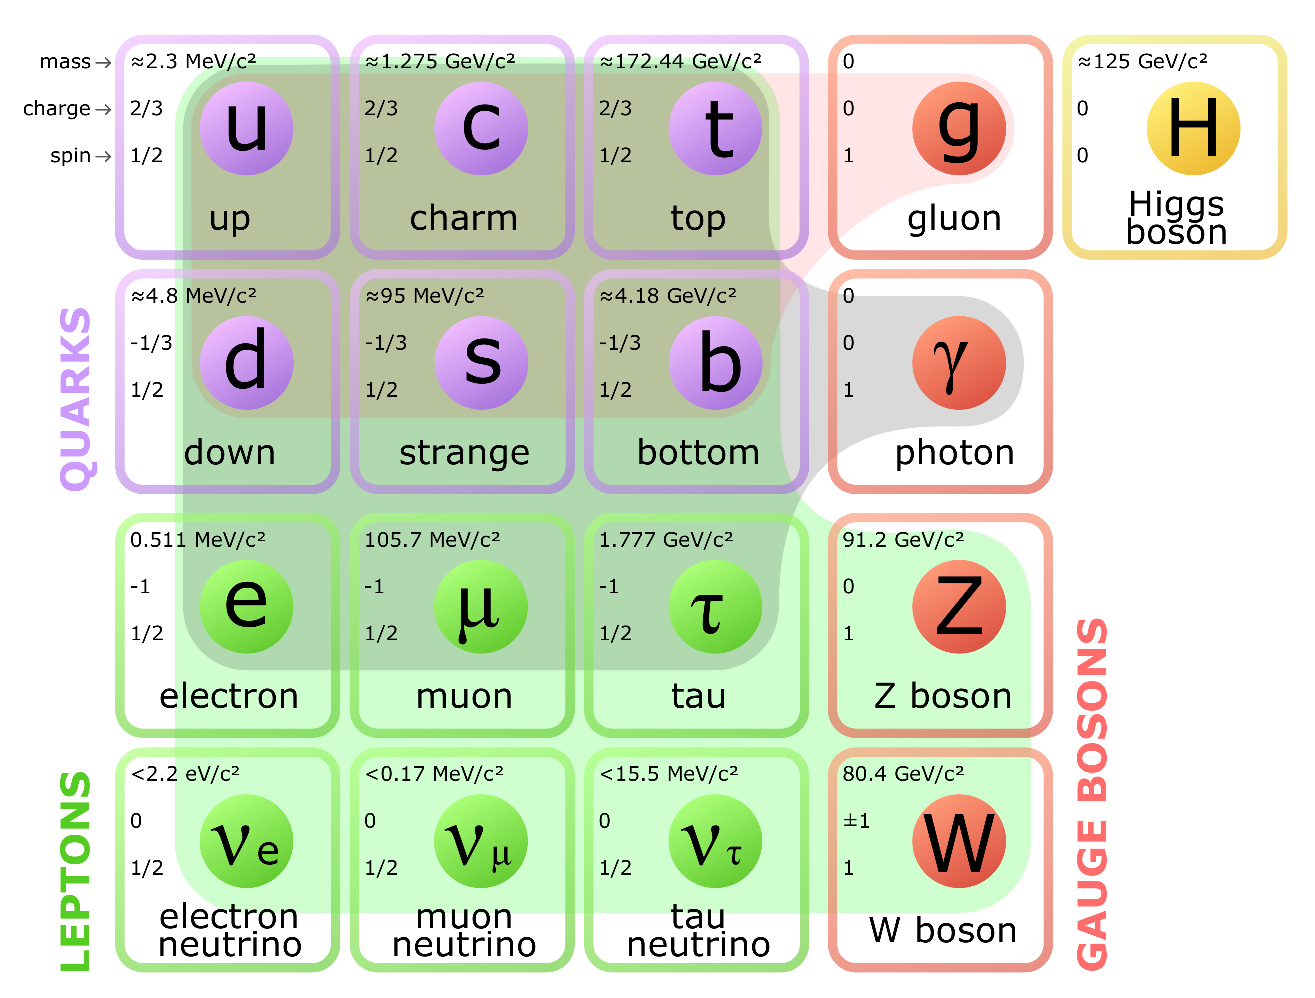
\includegraphics[width=0.6\textwidth]{figures/theory/Standard_Model_of_Elementary_Particles_modified_version.eps}
\caption[The particle content of the Standard Model]{The particle content of the Standard Model. Figure adapted from~\cite{wikipediaSM}.}
\label{fig:standard_model}
\end{centering}
\end{figure}


\section{The Lorentz group and particle states}

Lorentz group consists of coordinate transformations~$x^\mu = \Lambda^{\mu}_{\ \nu} x^\nu$~that preserve space-time intervals~$\mathrm{d}s^2 = \mathrm{d}x^\mu \Lambda^\mu_{\ \nu} x_\nu$, such that~$\mathrm{det}\ \Lambda = +1$~and~$\mathrm{sign}\ \Lambda^0_{\ 0} = +1$. The transformations form a group~$\mathrm{SO}^+(3,1)$, which can be decomposed~$\mathrm{SO}^+(3,1) \simeq \mathrm{SU}(2)_L \times \mathrm{SU}(2)_R$. The angular momenta~$(j_1, j_2)$~can be used to group the fields as scalars, left and right handed spinors and vectors. For example, a scalar field~$\phi(x)$~transforms as~$\phi(x) \rightarrow \phi(\Lambda^{-1} x)$, a vector field as~$A^\mu(x) \rightarrow \Lambda^\mu_{\ \nu} A^\nu(\Lambda^{-1}x)$~and a spinor field as~$\phi^\alpha(x) = S[\Lambda]^a_{\ \beta} \phi^\beta(x)$, where~$S[\Lambda]$~is a spinor representation built from~$4\times4$~Dirac~$\gamma$~matrices in the chiral representation.

These fields can be identified with particle states, which have a definite mass~$m$~and spin~$s$. Particles with integer spin follow Bose-Einstein statistics and are therefore called bosons, whereas particles with half-integer follow Fermi-Dirac statistics and are called fermions. 

\section{Relativistic quantum mechanics}
After having identified quantum fields with definite Lorentz transformation properties as central to QFT, the next step is to derive dynamical relations for the free fields in order to describe the propagation of free particles.

The Klein-Gordon wave equation,

\begin{equation}
\label{eq:theory_klein_gordon}
(\partial^\mu \partial_\mu + m^2) \psi = 0
\end{equation}
which can be derived from Einstein's energy-momentum relation~$E^2 = \vec{p}^2 + m^2$~by replacing energy and momentum with operators acting on the wavefunction~$\psi$, is a manifestly Lorentz-invariant relation between energy and momentum for the quantum mechanical wavefunction. However, it admits solutions with negative energy and negative probability densities, which are unphysical.

These negative-probability states led Dirac to search for a relation linear in~$\hat{\mathbf{p}}$~and~$E$, which resulted in the Dirac equation:

\begin{equation}
\label{eq:theory_dirac}
i (\gamma^\mu \partial_\mu - m) \psi = 0
\end{equation}
where~$\gamma^\mu$~are the~$4\times4$~Dirac~$\gamma$-matrices which satisfy the Clifford algebra anti-commutation relation~$\{ \gamma^\mu, \gamma^\nu \} = \gamma^\mu \gamma^\nu + \gamma^\nu \gamma^\mu = 2 g^{\mu\nu} \mathbb{I}$~and~$\psi$~is a four-component spinor. Using~\cref{eq:theory_dirac}, we can describe the dynamics, spin and magnetic momentum of free spin-half fermions. The probability densities predicted by Dirac's equation are now positive, but it still admits solutions with negative energy. In the Feynman-Stückelberg interpretation, these~$E<0$~particles can be interpreted as negative-energy particles moving backwards in time or equivalently anti-particles moving forwards in time. The predictions by Dirac's equation were spectacularly confirmed by the discovery of the positron in 1932~\cite{anderson1933positive}.

Both of these equations of motion can be derived using the principle of least action:

\begin{equation}
\label{eq:theory_action}
S = \int \mathrm{d}^4x\ \mathcal{L}_{\mathrm{free}},\ \delta S = 0,
\end{equation}
where~$\mathcal{L}_{\mathrm{free}}$~is the Lagrangian density for non-interacting fields. The Dirac action for a single free spinor field can be written as

\begin{equation}
\label{eq:theory_kg_lagrangian}
\mathcal{L}_{\mathrm{Dirac}} = \bar{\psi} i \gamma^\mu \partial_\mu \psi - m \bar{\psi} \psi,\ \bar{\psi} = \psi^\dagger \gamma^0
\end{equation}
and varied with respect to~$\psi$~to derive the Dirac equation.

\section{Interactions via gauge theory}
The concept of interactions mediated by fields is central to QFT and they can be described by requiring the Lagrangian to have additional symmetries. In particular, if we require the laws of physics to be invariant under local transformations~$\psi(x) \rightarrow U(x) \psi(x)$, where the continuous and differentiable transformations~$U(x)$~form Lie groups, then additional degrees of freedom corresponding to the mediator fields or gauge bosons are naturally incorporated in the Lagrangian.

\subsection{Quantum Electrodynamics}
For the~$\mathrm{U}(1)$~symmetry, which corresponds to the transformation~$\psi(x) \rightarrow e^{i q\varphi(x)} \psi(x)$, the derivative in the momentum operator in~\cref{eq:theory_kg_lagrangian} needs to be changed to

\begin{equation}
\partial_{\mu} \rightarrow \partial_{\mu} + i q A_{\mu}
\end{equation}
in order for the Lagrangian to be invariant under this symmetry. The field~$A_{\mu}$~is a massless gauge boson with spin 1 that is coupled to the fermion field~$\psi$~via a coupling constant~$q$~in the term~$q \gamma^\mu A_\mu \psi$. The formulation of quantum electrodynamics (QED) as a gauge theory generated by the Abelian group~$\mathrm{U}(1)_{\mathrm{EM}}$~was first done by Tomonaga, Feynman and Schwinger. In QED, the spinor~$\psi$~is associated to the electron, the vector~$A_\mu$~to the photon and~$q$~is the electric charge of the fermion. 

In order to compute observable decay rates or scattering cross sections under an interacting Hamiltonian~$H$, we use Fermi's golden rule, which relates the scattering rate~$\Gamma_{fi}$~to the transition matrix element between the initial and final state derived using perturbation theory:

\begin{equation}
\label{eq:transition_matrix}
\mathcal{M}_{fi} = \langle \psi_f | H | \psi_i \rangle.
\end{equation}

The matrix element~\cref{eq:transition_matrix} is a Lorentz scalar and can be explicitly computed from the Lagrangian using Feynman rules, where we represent each term in the perturbation expansion of~\cref{eq:transition_matrix} as a graphical diagram with the ingoing and outgoing lines, the vertices and the propagators are associated with quantities that are specified by the Lagrangian. The QED interaction vertex thus allows us to construct diagrams corresponding to any QED interaction and calculate scattering cross sections for processes such as electron-electron scattering, as depicted on~\cref{fig:theory_qed}.

\begin{figure}
\begin{centering}
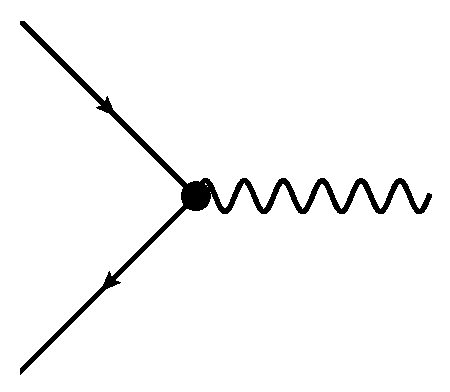
\includegraphics[width=0.3\textwidth]{figures/theory/qed_vertex.eps}
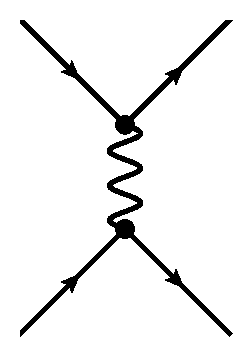
\includegraphics[width=0.2\textwidth]{figures/theory/qed_process.eps}
\caption{The QED vertex and a representative process.}
\label{fig:theory_qed}
\end{centering}
\end{figure}

It is remarkable that the gauge theory formulation of QED allows us to both recover Maxwell's equations of electromagnetism and predict the anomalous electric dipole moment of the electron, which has been confirmed to be accurate to about one part per billion. This underscores the predictive power of symmetries in the SM.

\subsection{Quantum chromodynamics}
\label{sec:theory_qcd}
The interaction of quarks and gluons can be described by the theory of quantum chromodynamics (QCD), which arises from the invariance of the Lagrangian under a local~$\mathrm{SU}(3)_C$~symmetry, where C stands for a colour charge that is~$N_c$-valent, with~$N_c = 3$~in the SM. The spinor field transforms under this group as

\begin{equation}
\psi(x) \rightarrow \psi'(x) = \exp \bigl[ i g_s \alpha^a(x) T^a \bigr] \psi(x)
\end{equation}
where~$T_a$~are the generators of the group represented by the~$3\times3$~Gell-Mann matrices~$\lambda^a$~as~$T_a = \frac{1}{2} \lambda^a$,~$g_s$~is the gauge coupling and~$\alpha^a(x)$~are the local gauge transformations corresponding to the 8 generators. The derivative can then be written as


\begin{equation}
\label{eq:theory_qcd_deriv}
\partial_\mu \rightarrow \partial_\mu + i g_s G^a_\mu T^a
\end{equation}
where~$G^a_\mu = \partial_\mu \alpha^a(x)$~must transform as~$G^a_\mu \rightarrow G^a_\mu - \partial_\mu \alpha^a - g_s f_{ijk} \alpha^i G^j_\mu$. The last term arises due to the non-Abelian nature of QCD, which means that the generators~$T^a$~do not commute, but are instead related through the structure constants:~$[T^a, T^b] = 2 i f_{abc} T^c$. The Lagrangian for a single quark field can then be written as

\begin{equation}
\label{eq:theory_quark_lagrangian}
\mathcal{L}_{\mathrm{quark}} = \bar{\Psi} (i \gamma^\mu \partial_\mu - m + g_s \gamma^\mu G^a_\mu T^a) \Psi = 0
\end{equation}
and we can associate~$G^a_\mu$~to the gluons and note that~$\Psi = (\psi_i)$~have 3 components corresponding to colour states, each of which is a 4-component Dirac spinor. The QCD quark-gluon interaction vertex is then

\begin{equation}
g_s \gamma_\mu T^a G^a_\mu.
\end{equation}

At this stage,~$G^a_\mu$~is simply a field associated with external sources, which can be made dynamical by adding a gauge-invariant term

\begin{equation}
\mathcal{L}_{\mathrm{gauge}} = - \frac{1}{2} \mathrm{Tr}\ [F^{\mu\nu} F_{\mu\nu}] 
\end{equation}
to the QCD Lagrangian, where~$F_{\mu\nu} = \partial_\mu G_\nu - \partial_\nu G_\mu + i g_s [G_\mu, G_\nu]$~with~$G_\mu = G_\mu^a T^a$~is the QCD gluon field strength tensor.

The~$\mathrm{SU}(3)_{\mathrm{C}}$~symmetry of QCD thus implies the existence of a conserved colour charge, which is exchanged between quarks by 8 gluons in QCD vertices. As free quarks have not been experimentally detected, the colour charge is hypothesised to be confined, such that quarks are only observed bound to colourless hadrons. Furthermore, this means that hadrons have to be colour singlets, which for baryons, composed of 3 quarks, implies that the colour wavefunction must be totally antisymmetric under the exchange of any two quarks, since the colour  singlet~$\psi_c = \frac{1}{\sqrt{6}} (rgb - rbg + gbr - grb + brg - bgr)$~from the decomposition~$\mathbf{3}\otimes \mathbf{3} \otimes \mathbf{3} = \mathbf{10} \oplus \mathbf{8} \oplus \mathbf{8} \oplus \mathbf{1}$~is totally antisymmetric.

In order to describe the phenomenology of high-energy interactions of protons, we thus need an effective model for building hadrons out of the elementary constituents of QCD - the quarks and gluons.

\section{The parton model}
Through the study of deep inelastic scattering (DIS) experiments, where an electron transfers sufficient energy~$Q^2$~to a proton for it to break up in the reaction~$\mathrm{e}^- \mathrm{p} \rightarrow \mathrm{e}^- \mathrm{X}$, it was possible to establish that the electrons scatter elastically off point-like spin-half constituents of the proton, the partons. This can be seen as an analogy to the Rutherford experiment, where electrons were scattered off the nucleus of an atom to reveal the pointlike structure of the nucleus within. By identifying the partons as the quarks from QCD, electron-proton interactions can thus be described in terms of the more fundamental electron-quark interactions.

Furthermore, by measuring the~$Q^2$-dependence of the QCD coupling constant~$\alpha_s(Q^2) = q^2 / 4\pi$~ experimentally and from theoretical considerations of QCD~\cite{PhysRevLett.30.1343,PhysRevLett.30.1346}, it has been possible to establish that at very high~$Q^2$, the coupling constant~$\alpha_S(Q^2)$~becomes vanishingly small, such that quarks can be treated as free particles in the asymptotic limit. The~$Q^2$-dependence of~$\alpha_s$~can be seen on~\cref{fig:theory_alphas_running}, confirming the QCD prediction of asymptotic freedom. Only when the coupling~$\alpha_S(Q^2)$~is sufficiently small can perturbative QCD (pQCD) be used to compute cross-sections of the underlying processes. At a momentum scale comparable to typical hadron sizes~$\Lambda_{\mathrm{QCD}} = 0.1\dots0.3$~GeV, the coupling constant becomes unphysical, implying the breakdown of perturbative QCD at~$Q < \Lambda_{\mathrm{QCD}}$.

\begin{figure}
\begin{centering}
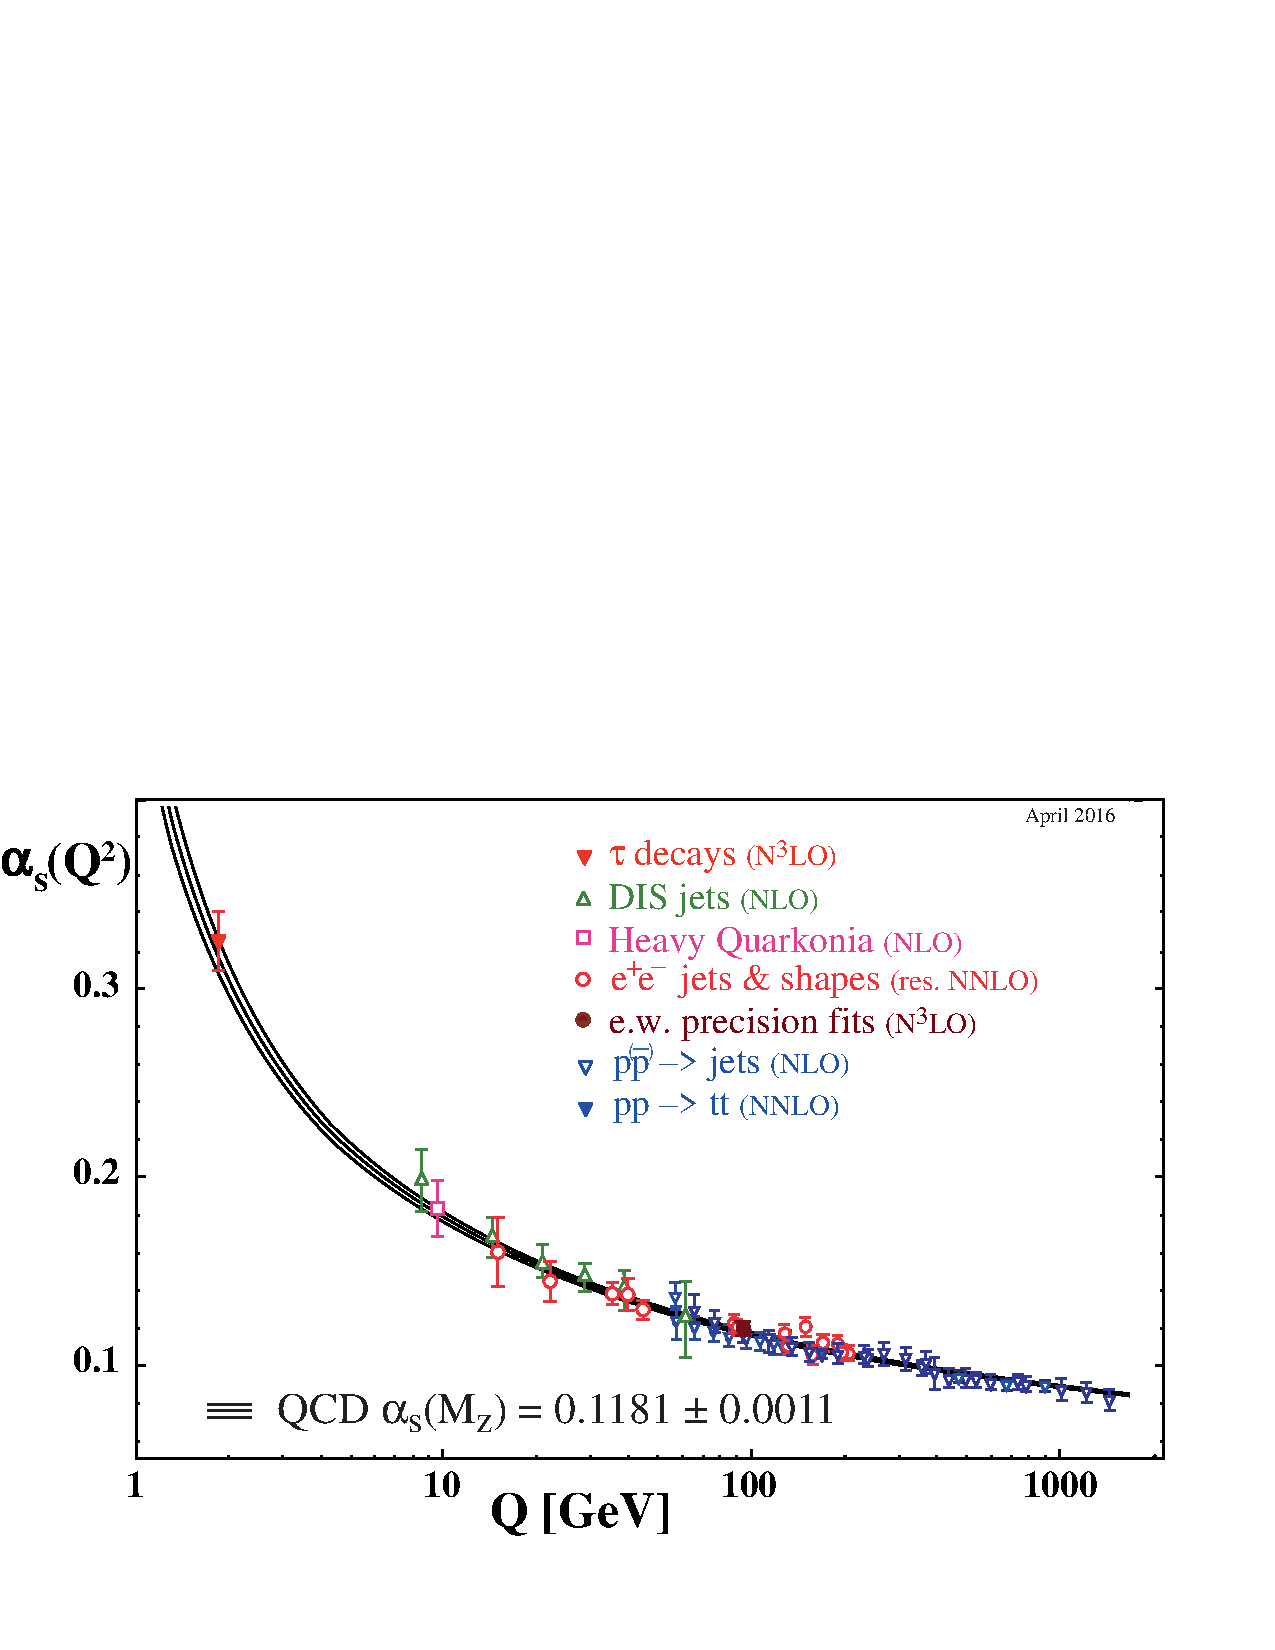
\includegraphics[width=1.0\textwidth]{figures/theory/asq-2015.pdf}
\caption[The measured values of~$\alpha_S(Q^2)$ compared to NLO QCD]{The measured values of~$\alpha_S(Q^2)$, compared to the prediction from NLO QCD. Figure from~\cite{Patrignani:2016xqp}.}
\label{fig:theory_alphas_running}
\end{centering}
\end{figure}

In order to model a proton-proton interaction with a hard scattering, such as the Drell-Yan process~$\mathrm{q} \bar{\mathrm{q}} \rightarrow \ell^+ \ell^-$~at high~$Q^2$, we describe the protons in terms of parton distribution functions~(PDFs)~$f_a^{\mathrm{p}}(x)$, which specify the fraction of proton momentum~$x$~carried by a quasi-free constituent quark or gluon~$a$~and factorize the proton-proton interaction to a hard interaction between quarks and gluons, as depicted on~\cref{fig:theory_pdf_factorization}. This allows us to write the factorized cross-section as


\begin{equation}
\label{eq:theory_pdf_factorization}
\mathrm{d}\sigma(\mathrm{p}\mathrm{p} \rightarrow cd) = \int_0^1 \mathrm{d}x_1 \mathrm{d}x_2 \sum_{a,b} f_a^{\mathrm{p}}(x_1, \mu_F^2) f_b^{\mathrm{p}}(x_2, \mu_F^2)\ \mathrm{d}\hat{\sigma}^{ab \rightarrow cd} (Q^2, \mu_f^2),
\end{equation}
which is evaluated at the factorization scale~$\mu_f^2$. The PDFs have to be determined from experimental data. As the proton is a dynamical system of bound quarks that interact strongly via virtual gluon exchange, the protons are found to contain a \textit{sea} of gluons and quarks and anti-quarks from the vacuum fluctuations of~$g \rightarrow \mathrm{q} \bar{\mathrm{q}}$~in addition to the up and down \textit{valence} quarks expected from flavour symmetry.

\section{Flavour states of hadrons}
The known quarks of the SM come in 6 different flavours, grouped into 3 generations: up and down (I), charm and strange (II), top and bottom (III). The underlying reason for the SM having exactly 3 generations is unknown, but an approximate symmetry between flavours allows us to predict allowable hadronic states that can be formed from quarks. Strong interaction is approximately invariant under~$\mathrm{u} \leftrightarrow \mathrm{d}$~exchange, which implies an~$\mathrm{SU}(2)$~flavour symmetry. This group has 3 generators~$\hat{T}_i$~that can be represented as~$2\times2$~Pauli spin matrices. This means that for a given flavour state~$\psi$, the quantized isospin~$I_3 \leftrightarrow \hat{T}_3$~and the total isospin~$I \leftrightarrow \hat{T}^2$~are conserved in analogy to spin, and can therefore be used to label composite flavour states of quarks as~$\phi(I, I_3)$.

We can construct the flavour wavefunction proton, which contains 3 valence quarks (uud), by combining 3 isospin doublets~$\mathbf{2} \otimes \mathbf{2} \otimes \mathbf{2}$, which results in a spin~$I=3/2$~quadruplet and two spin~$I=1/2$~doublets~$\phi_A=\frac{1}{\sqrt{2}}(\mathrm{udu} - \mathrm{duu})$~and~$\phi_S = \frac{1}{\sqrt{6}}(2 \mathrm{uud} - \mathrm{duu} - \mathrm{udu})$, that are (anti)symmetric under the exchange of the first two quarks. The proton wavefunction is then a superposition of the two flavour doublets, multiplied by the corresponding (anti)symmetric wavefunctions for the spin states, such that the flavour-spin wavefunction is completely symmetric under the exchange of any two quarks. This, combined with the completely antisymmetric colour wavefunction as described in~\cref{sec:theory_qcd}, guarantees that the proton wavefunction is completely antisymmetric under the exchange of any two quarks.

The~$\mathrm{SU}(2)$~isospin symmetry of flavour allows us to write down the wavefunction of the proton in the ground state and predict the existence and approximate masses of the excited states such as the~$\Delta$-baryons. It is not an exact symmetry, as illustrated by the difference in the proton and neutron masses, which should vanish under precise~$\mathrm{SU}(2)$~isospin symmetry, but nevertheless underscores the role of symmetries in describing hadronic states.

\section{Electroweak unification}
The parity-violating weak force, which couples neutrinos to charged leptons and is responsible for radioactive~$\beta$-decay, can be associated to a~$\mathrm{SU}(2)_L$~gauge symmetry. The left-handed fermions form doublets~$(\nu_L, \mathrm{\ell}_L)$~for leptons and~$(q_L, q'_L)$~for quarks, whereas right-handed fermions are singlets under weak isospin. The generators~$T^i$~of~$\mathrm{SU}(2)_L$~are related to the 3 Pauli matrices~$T_i = \frac{1}{2}\sigma_i$, which can then be associated to 3 vector boson fields that mediate the weak force:~$W^+_\mu, W^-_\mu, W^0_\mu$.

The weak and electromagnetic forces both suggest an electrically neutral boson, so the physically observed states of the photon and the Z-boson must be a superposition of the two, implying a connection between the weak and electromagnetic forces. In the Glashow-Weinberg-Salam theory of electroweak unification, the Lagrangian is symmetric under the group~$\mathrm{SU}(2)_L \times \mathrm{U}(1)_Y$, whereas the vacuum state is symmetric only under the QED gauge symmetry~$\mathrm{U}(1)_{\mathrm{EM}}$. In the unified theory, it is necessary to introduce a new quantum number~$Y$, the hypercharge, which is equal for both both components of the~$\mathrm{SU}(2)_L$~doublets, so that the left-handed doublets would be invariant under both~$\mathrm{SU}(2)_L$~and~$\mathrm{U}(1)_Y$~symmetries. The observed electric charges of the fermions are then related to the weak hypercharge~$Y$~and weak isospin~$I_3$~by~$Q = I_3 + Y/2$.

The theory of electroweak unification was confirmed by the discovery of the Z-boson at LEP, which couples to both left-handed and right-handed fermions. This has allowed the weak mixing angle~$\theta_W$~between the neutral vector boson states to be measured. Furthermore, the decay~$\mathrm{Z} \rightarrow \nu \bar{\nu}$~can be used to determine the number of light neutrino generations by measuring the total width of the Z-boson~$\Gamma_Z$~and the decay widths to visible fermions - the charged leptons~$\mathrm{e}^\pm, \mathrm{\mu}^\pm, \mathrm{\tau}^\pm$~and quarks. The principle of local gauge invariance has great predictive power for the overall structure of the observed interactions, but it does not account for the mechanism by which electroweak symmetry breaking (EWSB) is realized nor the mass of the~$\mathrm{W}^\pm$~and Z bosons, which would violate gauge invariance. In order to incorporate these phenomena, we turn to the Higgs mechanism.

\section{Higgs mechanism}
We can introduce mass terms for the heavy gauge bosons by coupling them to two complex scalar fields arranged in a weak isospin doublet~$\phi = \frac{1}{\sqrt{2}} (\phi^+\ \phi_0)^T$. The Lagrangian density for this scalar field is~$\mathcal{L}_{\phi} = (\partial_\mu \phi)^\dagger (\partial^\mu \phi) - V(\phi)$, where the Higgs potential~$V(\phi) = \mu^2 (\phi^\dagger \phi) + \lambda (\phi^\dagger \phi)^2$~has degenerate minima~$\phi^\dagger \phi = v^2 / 2 = -\mu^2/2\lambda$~for~$\mu^2 < 0$. If the physical vacuum state does not have the same symmetries as the Lagrangian, then it is possible to introduce gauge-invariant mass terms for gauge bosons and fermions.

The Higgs field couples to the gauge fields through the kinetic term~$(\partial_{\mu} \phi)^\dagger (\partial^\mu \phi)$, which is made gauge invariant by~$\partial_\mu \rightarrow D_\mu = \partial_mu + i g_W T^a W_\mu^a + i g' Y B_\mu / 2$. The vacuum state is then chosen to be~$\langle 0|\phi|0\rangle = \frac{1}{\sqrt{2}} (0\ v)^T$, so the Higgs field can be expanded around the vacuum, resulting in a massive scalar field~$\eta$~and 3 massless Goldstone fields~$\phi_1, \phi_2, \phi_3$. The Goldstone bosons are removed from the Lagrangian by fixing the gauge, such that they correspond to the degrees of freedom of longitudinal polarization states of the Z and~$\mathrm{W}^\pm$~bosons. The masses of the gauge bosons can then be written as~$M_W = \frac{1}{2} g_W v$~and~$m_Z = \frac{1}{2} g_W v / \cos{\theta_W}$. The theory of EWSB predicts~$m_W / m_Z = \cos{\theta_W}$, which has been confirmed experimentally~\cite{ALEPH:2005ab}.

The explicit mass terms for fermions in the form of~$m \bar{\psi} \psi$~are not gauge invariant. By arranging the left-handed fermions in a~$\mathrm{SU}(2)$~doublets~$L$~and the right-handed fermions in singlets~$R$, the mass terms for Dirac fermions can be introduced through spontaneous symmetry breaking through the terms~$y_f \bar{L}\phi R + y_f (\bar{L}\phi R)^\dagger$~for down-type leptons $e^\pm$, $\mu^\pm$, $\tau^\pm$ and quarks $\mathrm{d}$, $\mathrm{s}$~and $\mathrm{b}$. The constant $y_f = \sqrt{2} m_f / v$ is the Yukawa coupling of the fermions, which has to be fixed from the experimental determination of the masses. A conjugate Higgs doublet~$\phi_c = -i\sigma_2 \phi^*$~is used to give the mass terms for the up-type quarks. From this mechanism, the Yukawa coupling of the top quark is found to be compatible with unity, a scale very different from the rest of the quarks.

To summarize, the Higgs mechanism can accommodate the observed masses of heavy gauge bosons and fermions in a unified electroweak theory. It predicts the existence of a massive scalar boson, which can decay to fermions through~$\mathrm{H} \rightarrow \mathrm{f} \bar{\mathrm{f}}$~or bosons through~$\mathrm{H} \rightarrow \mathrm{W}^+ \mathrm{W}^-$ and ~$\mathrm{H} \rightarrow \mathrm{Z} \mathrm{Z}$, and through higher-order processes to $\mathrm{H} \rightarrow \gamma \gamma$.

\section{Higgs phenomenology at the LHC}
The discovery of the Higgs boson with $m_H \simeq 125$~GeV in 2012 at the LHC by the CMS~\cite{Chatrchyan:2012xdj} and ATLAS~\cite{Aad:2012tfa} collaborations confirmed the basic mechanism of EWSB and mass generation and completed the particle spectrum of the SM. Following this, a new experimental and theoretical program has opened in experimentally verifying the properties of the Higgs boson. In particular, it should be established whether Higgs boson couples to SM gauge bosons and fermions as expected by observing these processes directly. In Run I of the LHC, the couplings to gauge bosons have been established with significant sensitivity, however, to be able to determine the couplings to fermions, Run II data of the LHC will be necessary.

Beyond establishing the existence of the predicted production and decay channels, a crucial test of the Higgs mechanism is determining the coupling strengths of the new scalar to SM fields and comparing them to the predictions. The top quark Yukawa coupling~$y_t$~, which is much larger than that of lighter quarks, determines the evolution of he Higgs self coupling~$\lambda$~under renormalization and is currently only known indirectly.

\section{Production modes}
The main production modes of the Higgs boson at the LHC, show on~\cref{fig:higgs_xs}, are through gluon-gluon fusion (ggF), with a cross-section of~$\sigma_{\mathrm{ggF}} = 48.6^{+2.2}_{-3.6}\pm1.6~(\mathrm{PDF})$~pb, weak or vector boson fusion (VBF) with a cross-section $\sigma_{\mathrm{VBF}} = 3.78^{+2\%}_{-2\%}$~pb, associated production with vector bosons (VH) with~$\sigma_{\mathrm{WH}} = 1.37^{+2\%}_{-2\%}$~pb,~$\sigma_{\mathrm{ZH}} = 0.88^{+5\%}_{-5\%}$~pb and the associated production with top quark pairs (\ttH) with $\sigma_{\ttH} = 0.51^{+9\%}_{-13\%}$~pb or with a single top quark~(tH).

\begin{figure}
\begin{centering}
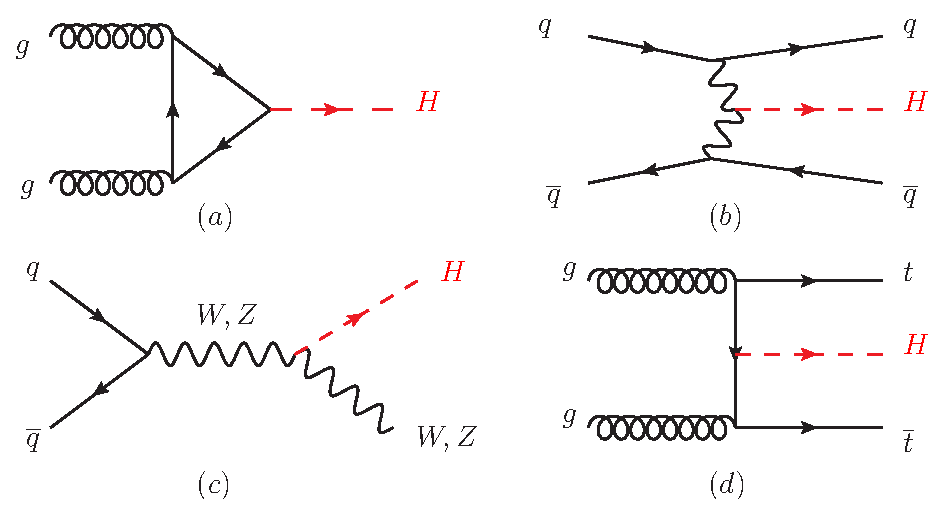
\includegraphics[width=0.6\textwidth]{figures/theory/PDG.eps}
\caption[Tree-level Feynman diagrams for Higgs production]{The generic tree-level Feynman diagrams for Higgs boson production: the gluon fusion process (ggF) on (a), vector boson fusion on (b), associated production with vector bosons (VH) on (c) and associated production with top quarks (\ttH) on(d). Figure from the PDG~\cite{Patrignani:2016xqp}.}
\label{fig:higgs_production}
\end{centering}
\end{figure}

\begin{figure}
\begin{centering}
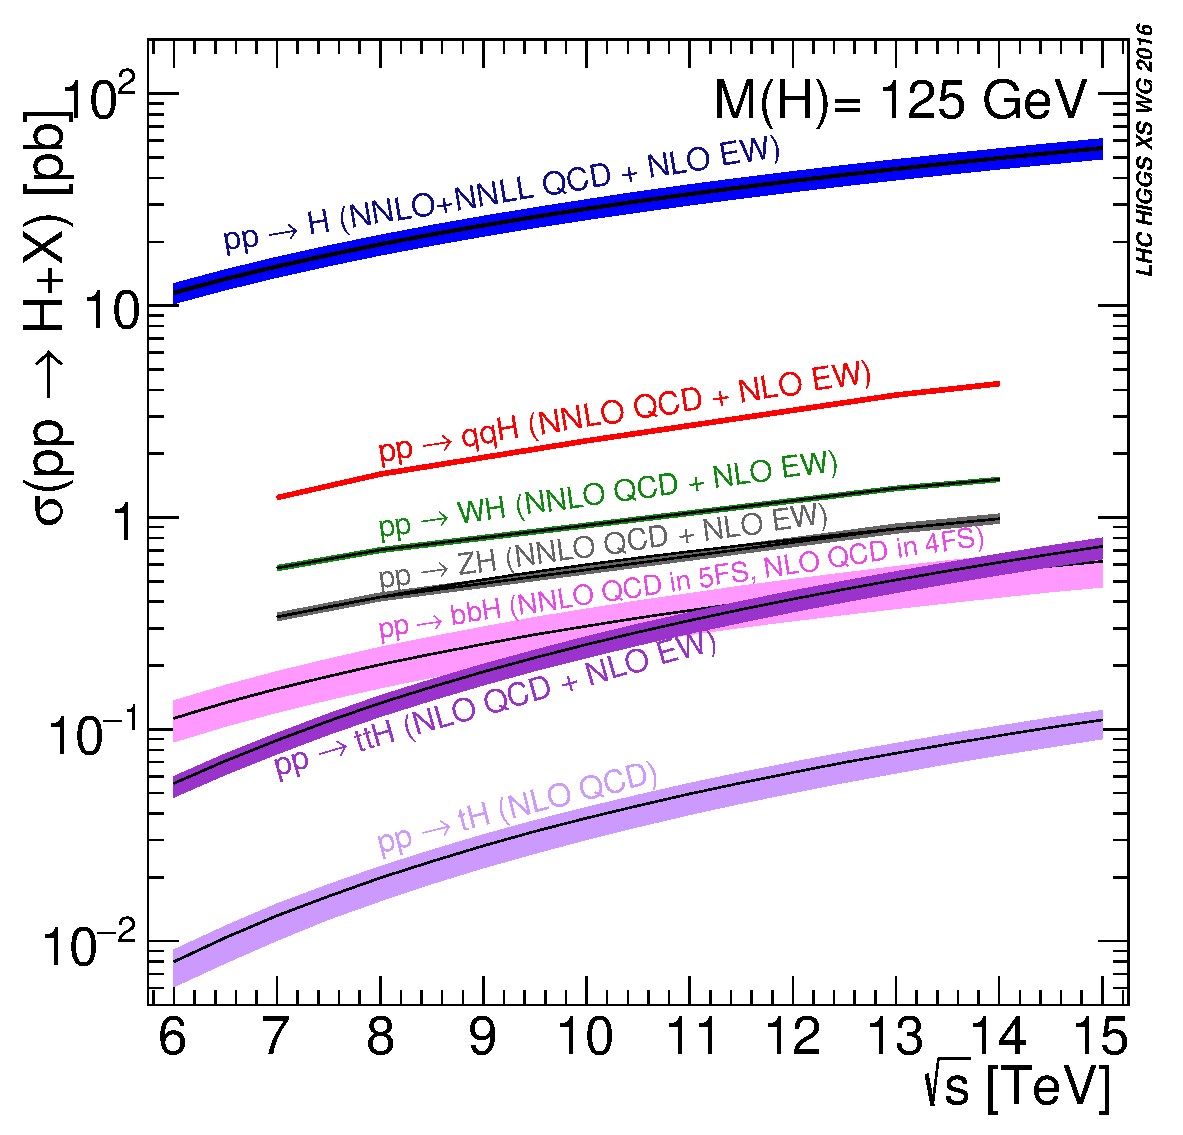
\includegraphics[width=0.4\textwidth]{figures/theory/Higgs_XS_7-14TeV-2016.eps}
\caption[The production cross-section of the Higgs boson]{The production cross section of the SM Higgs boson with $m_H = 125$~GeV as a function of~$\sqrt{s}$ along with theoretical uncertainties. Figure from the PDG~\cite{Patrignani:2016xqp}.}
\label{fig:higgs_xs}
\end{centering}
\end{figure}

The ggF production proceeds predominantly via the top quark loop and is known to N3LO. This was the main production mode for the initial observation and discovery with the~$\mathrm{H} \rightarrow \gamma \gamma$,~$\mathrm{H} \rightarrow \mathrm{W}^+\mathrm{W}^- \rightarrow \mathrm{e} \mathrm{\nu} \mathrm{\mu} \mathrm{\nu}$~and~$\mathrm{H} \rightarrow \mathrm{Z}\mathrm{Z} \rightarrow 4\ell$ signatures, which are important for the measurement of the production cross-section,~$J^P$~and mass of the Higgs boson. It also serves as an indirect verification of the top-Higgs Yukawa coupling, due to the presence of the top quark loop in ggF. For the direct decay of the Higgs boson to fermions, additional production modes have to be considered. The VBF mode, where two (anti)quarks scatter through the exchange of a weak boson in~$\mathrm{qq} \rightarrow \mathrm{qqH}$~is important both for discovery and determination of the couplings, as it can be distinguished from QCD background through the presence of two jets in the opposite forward regions of the detector originating from the scattered quarks. The VH mode allows the use of leptonic decays of the W/Z bosons to reduce the multijet background, such that this mode has recently been used to establish the~\Hbb~decay. While inclusive ggF measurements are already sensitive to the top quark Yukawa coupling~$y_t$, the~\ttH~and tH channels can be used to probe~$y_t$~directly, such that they provide an important independent verification of the mass generation mechanism for the top quark.

\section{Decay channels}
The Higgs boson decays to SM particles with decay widths~$\Gamma$~that are proportional to the mass of the daughter particles. For~$m_H
\simeq 125$~GeV, the dominant decay channels are the decay to bottom quarks~\Hbb~with a branching ratio~$\mathrm{BR} = \Gamma/\Gamma_{H} = 0.584 \pm 3.3\%$, the decay to an on-shell and an off-shell W-boson~$\mathrm{H}\rightarrow \mathrm{W} \mathrm{W}^*$~($\mathrm{BR} = 0.214\pm4.3\%$) and the decay to tau leptons~$\mathrm{H} \rightarrow \mathrm{\tau}^+ \mathrm{\tau}^-$~($\mathrm{BR} = 0.063 \pm 5.7\%$). Through loop-induced processes, which are enhanced by the large top quark mass, the Higgs boson can also decay to massless particles in the channels~$\mathrm{H} \rightarrow \mathrm{g} \mathrm{g}, \mathrm{\gamma}\mathrm{\gamma}$ with non-negligible branching fractions. The branching ratios for a SM Higgs boson as a function of~$m_H$~can be seen on~\cref{fig:higgs_br}.

\begin{figure}
\begin{centering}
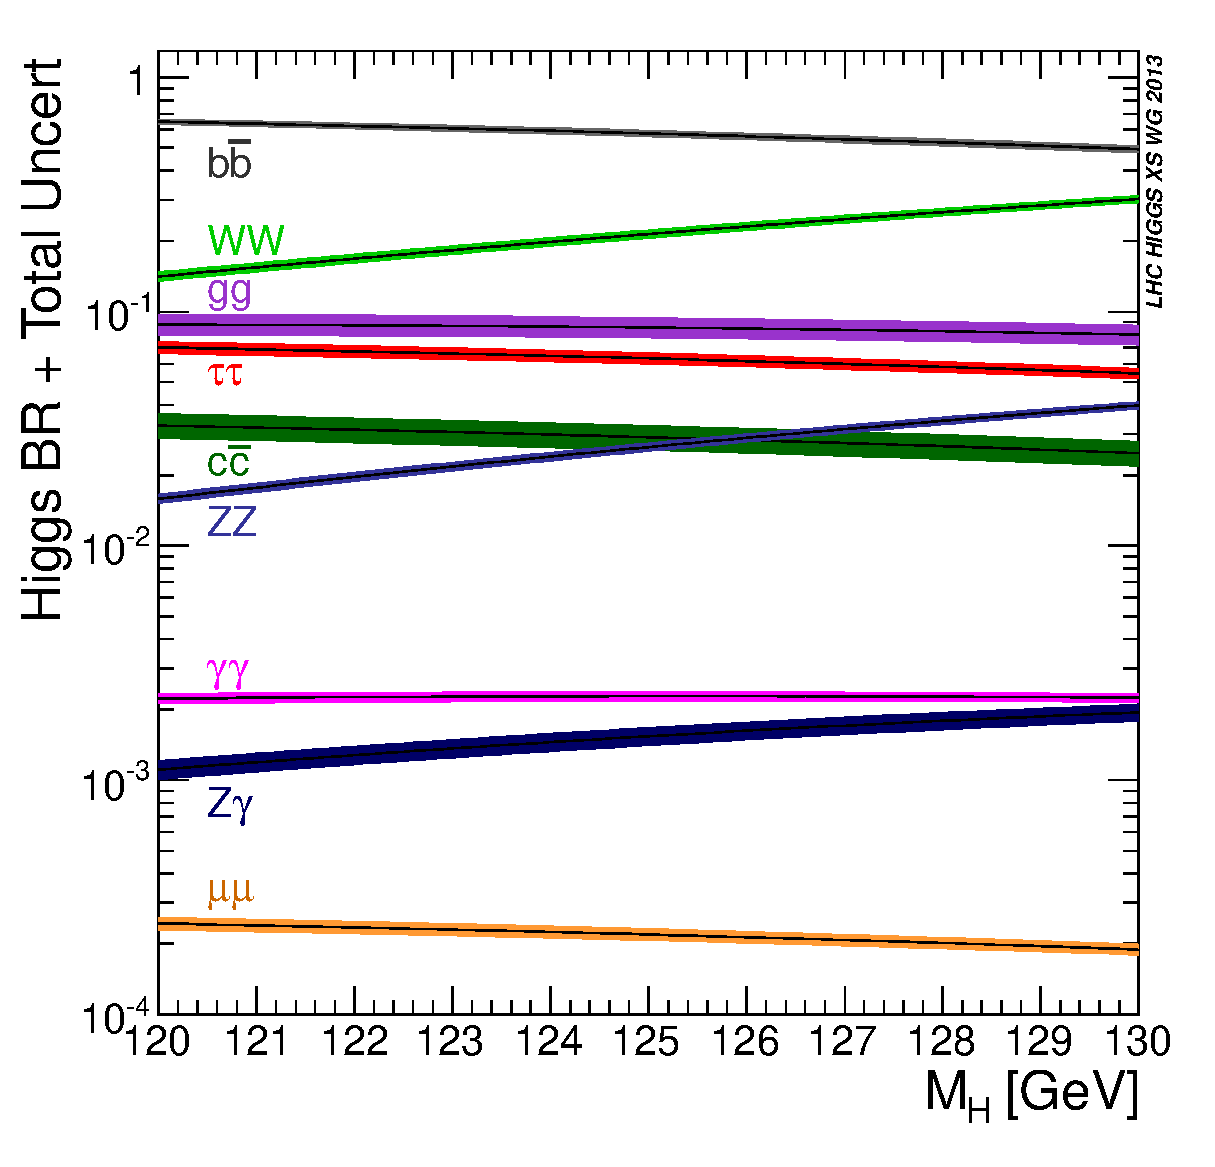
\includegraphics[width=0.4\textwidth]{figures/theory/higgs_br.eps}
\caption[The branching ratios of the Higgs boson]{The branching ratios of the SM Higgs boson around~$m_H = 125$~GeV along with the theoretical uncertainties. Figure from the PDG~\cite{Patrignani:2016xqp}.}
\label{fig:higgs_br}
\end{centering}
\end{figure}

\section{Experimental characterization}
Accurate predictions for the Higgs boson production cross sections and branching ratios for decays allow experimental data to be interpreted and the properties of the Higgs boson to be measured. The mass~$m_H$~has been measured most accurately in the~$\mathrm{H}\rightarrow\mathrm{\gamma}\mathrm{\gamma}$~and~$\mathrm{H} \rightarrow \mathrm{Z}\mathrm{Z} \rightarrow 4\ell$~channels, with a combined value of~$m_H = 125.09 \pm 0.21~(\mathrm{stat}.) \pm 0.11~(\mathrm{syst})$~GeV, dominated by statistical uncertainties, with the photon momentum scale uncertainties being the most significant systematic uncertainty~\cite{Aad:2015zhl}. The spin and parity~$J^P$~of the Higgs boson are probed independently of the mass and total cross section and are found to be compatible with the SM~$0^+$ hypothesis, excluding the pseudoscalar hypothesis at a~$98-99\%$ confidence level~\cite{Khachatryan:2014kca,Aad:2013xqa}. The width of the Higgs boson cannot be measured directly at the LHC, since the mass resolution in the diphoton and~$4\ell$~channels is $1-2$~GeV, 3 orders of magnitude larger than the expected SM line width $\Gamma_H = 4.2$~MeV. However, it can be constrained by comparing the on-shell and off-shell~$\mathrm{H} \rightarrow \mathrm{VV}$~cross sections, thus setting upper limits on~$\gamma_H$~that are around 5-6 times the SM value~\cite{Khachatryan:2014iha}.

It is important to experimentally confirm that the coupling strengths of the Higgs boson to SM particles correspond to those predicted by the SM. Any deviation from the values predicted by the standard Higgs mechanism could thus signal physics beyond the SM (BSM). The simplest way to experimentally characterize discrepancies in the couplings is the so-called~$\kappa$-framework~\cite{Heinemeyer:2013tqa}, where the couplings to SM particles are rescaled by factors~$\kappa_i$~for~$i \in \{\mathrm{Z}, \mathrm{W}, \mathrm{f}, \mathrm{g}, \mathrm{\gamma}, \mathrm{Z\gamma}\}$~which can be determined from signal strength~($\mu = \sigma / \sigma_{\mathrm{SM}}$)~measurements, without modifying the SM structure of the theory. In this formalism, the~\ttH~ signal strength modified is given by~$\mu_{\ttH} = \kappa_{\mathrm{t}}^2$. The CMS and ATLAS collaborations have extracted these signal modifier values from Run I data in a combined fit, with the results shown on~\cref{fig:higgs_kappa}. The results, while compatible with the SM, have significant uncertainties, in particular for~$\kappa_t$, thus paving the way for Run II measurements with improved sensitivity.

\begin{figure}
\begin{centering}
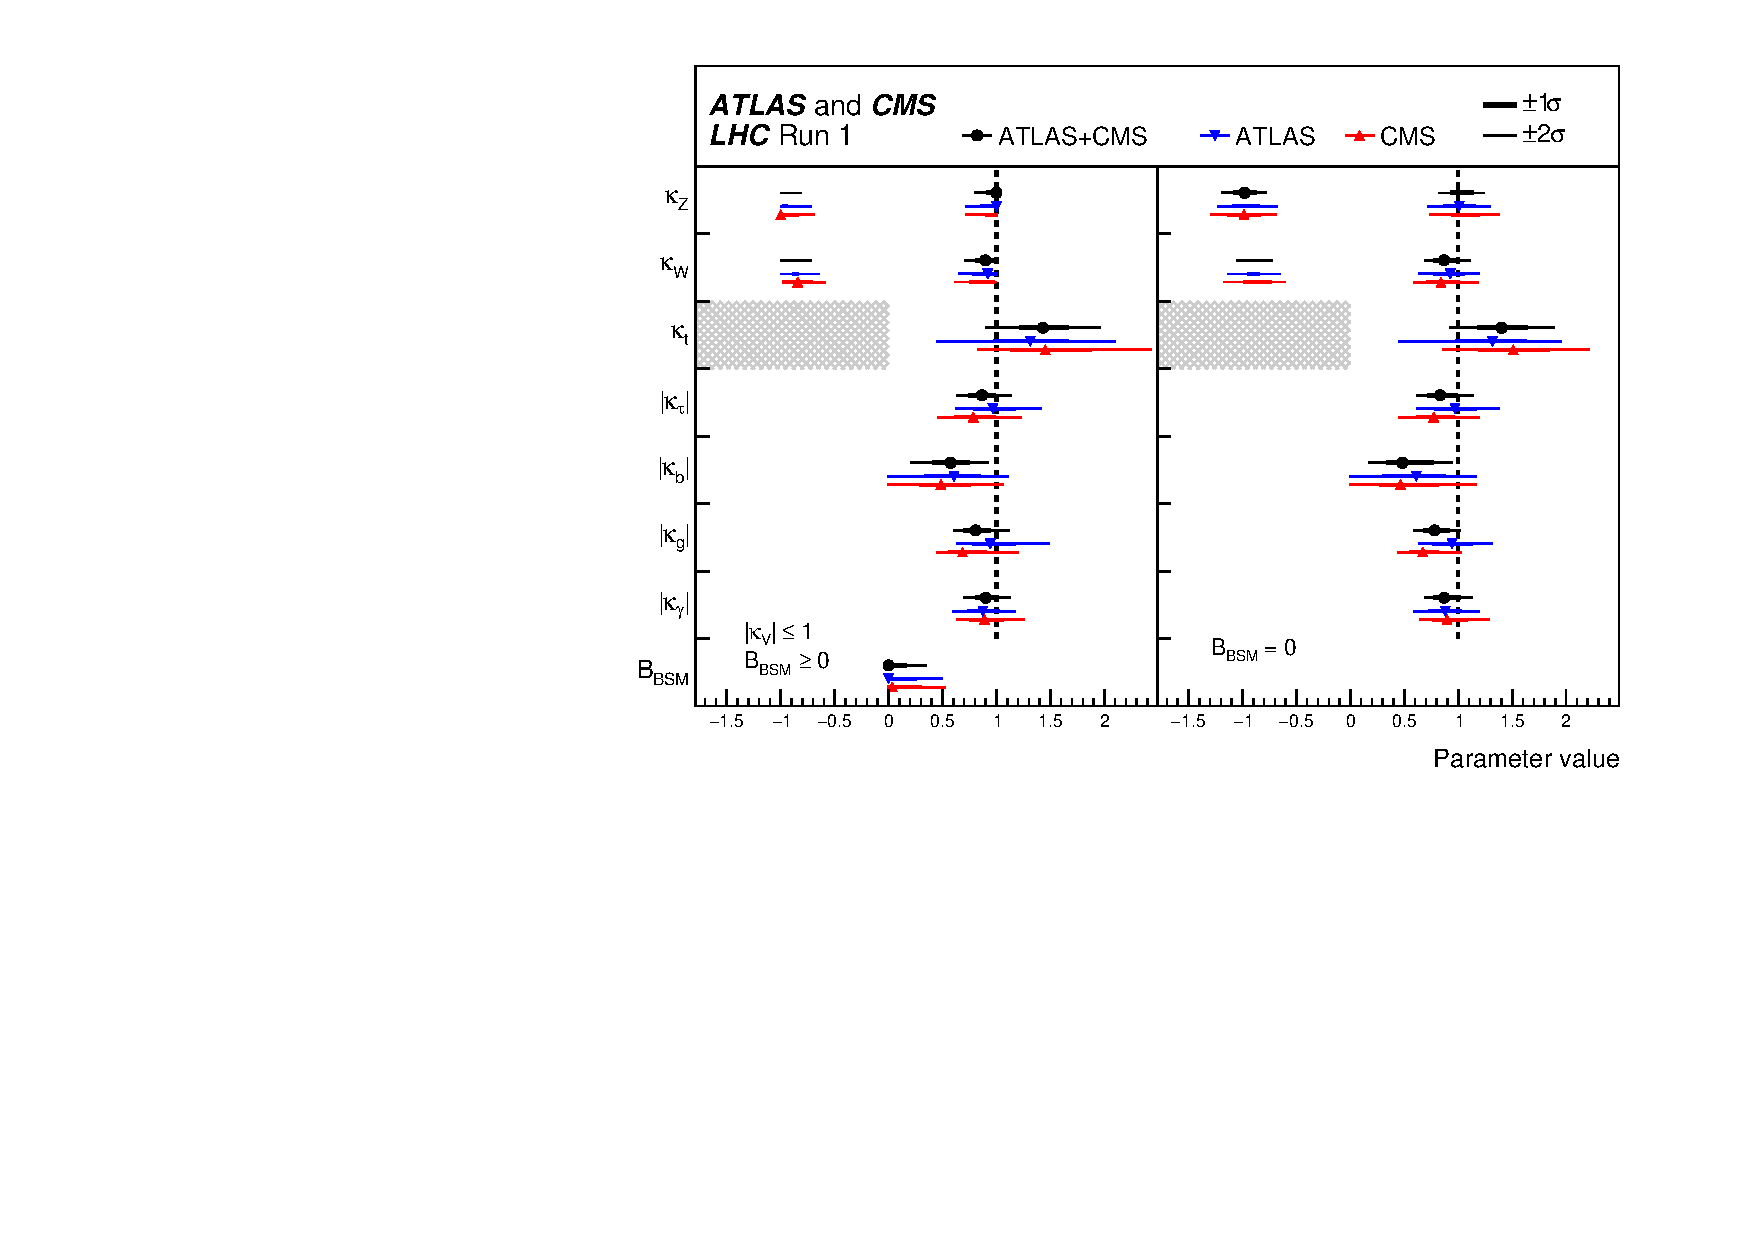
\includegraphics[width=0.8\textwidth]{figures/theory/CMS-HIG-15-002_Figure_015.pdf}
\caption[The Higgs signal strength modifier factors as measured by CMS and ATLAS]{The combined signal strength modified factors~$\kappa$~from the CMS and ATLAS collaborations with Run I data. Figure from~\cite{Khachatryan:2016vau}.}
\label{fig:higgs_kappa}
\end{centering}
\end{figure}

While the~$\kappa$-framework is relatively simple to apply for small deviations in signal strength, the clear short-coming of this approach is that any BSM physics would necessarily change the structure of the theory, rendering the results potentially invalid. In particular, the above approach assumes that the loop contributions in ggF and $\mathrm{H} \rightarrow \mathrm{\gamma} \mathrm{\gamma}$ are not modified by new physics. Furthermore, differences in kinematic distributions, such as the Higgs transverse momentum distribution, cannot be captured in the~$\kappa$~framework. Therefore, it has been suggested to use either Higgs pseudo-observables~\cite{Gonzalez-Alonso:2014eva} or effective field theories (EFT) to further parametrize any deviations from the SM.

\section{Top-Higgs coupling}
In the SM, the coupling between the top quark and Higgs boson is predicted to be~$y_t = \sqrt{2} m_t / v$, which can be verified independently through the measurement of Higgs boson production cross sections. This makes that the direct determination of the top-Higgs coupling in~\ttH~a test of the EWSB model at natural scale where~$y \simeq 1$.  

The top-Higgs coupling plays an important role in vacuum stability, since it controls the evolution of the self-coupling~$\lambda$~of the Higgs potential through renormalization evolution $\frac{\mathrm{d}\lambda}{\mathrm{d}\ln{\mu}}$, where it gives a quartic negative contribution. In particular, if~$y_t$~is sufficiently large but well within the bounds set by experimental uncertainties, the self-coupling~$\lambda$~becomes negative at a renormalization scale~$\mu$~below the Planck scale~$M_{\mathrm{Pl}} = \sqrt{\bar{h}c / G} \simeq 10^{19}~\mathrm{GeV}$, where gravitation becomes important in QFT. This means that the Higgs potential develops an additional minimum, which would possibly make the SM vacuum state metastable, depending on the exact values of~$m_H$~and~$m_t$~\cite{Degrassi:2012ry}. Since the scale where the scalar self coupling becomes negative depends strongly on~$y_t$, an accurate determination of~$y_t$~can help to pinpoint the scale of new physics in the absence of clear BSM signals~\cite{Bezrukov:2014ina}.

Furthermore, the top-Higgs coupling, which is purely scalar in the SM, can be extended quite generally to contain scalar and pseudoscalar interactions, making it possible to use results from~\ttH~for setting direct constraints on anomalous top-Higgs couplings~\cite{Kobakhidze:2016mfx}. Such anomalous couplings can arise from the two-Higgs doublet model that appears in several BSM scenarios, such as supersymmetry or axions~\cite{Branco:2011iw} or from models with a composite Higgs~\cite{Liu:2017dsz}.
\chapter{Experimental setup}
In this section, we will give an overview of the experimental setup of the Large Hadron Collider (LHC) and the Compact Muon Solenoid (CMS) experiment as it pertains to the~\ttH~search during Run II of the LHC. First, we will review the essential details of the LHC machine and the main experiments on the LHC ring. At the time of writing, the LHC, which is located at CERN nearby Geneva, is the highest-energy hadron collider in the world and the only experimental apparatus where Higgs bosons can be produced and studied directly. Next, we will discuss the CMS experiment, which is one of the two general-purpose detectors on the LHC ring. In particular, we will describe the subsystems and reconstruction algorithms of the detector that are crucial to the~$\ttH$~search.

\section{The Large Hadron Collider}
The LHC is a hadron collider situated in the 26.7-km tunnel of the Large Electron Positron (LEP) machine. The hadrons, either protons or heavy ions, are accelerated in several stages by the pre-accelerator complex of the LEP, shown on figure~\cref{fig:lhc_accelerators}. In the description that follows, we will consider only proton-proton collisions for concreteness. The protons are accelerated by the linear accelerator LINAC to 50~MeV, the proton synchrotron booster (PSB) to 1.4~GeV, the proton synchrotron (PS) to 26~GeV and by the super proton synchrotron to 450~GeV. The protons are injected in bunches of~$N_b = 1.15 \times 10^{11}$~protons per bunch into the main rings with a frequency of 40~MhZ, such that the nominal bunch spacing is 25~ns and there are~$n_b=2556$~bunches per beam.

\begin{figure}
\begin{centering}
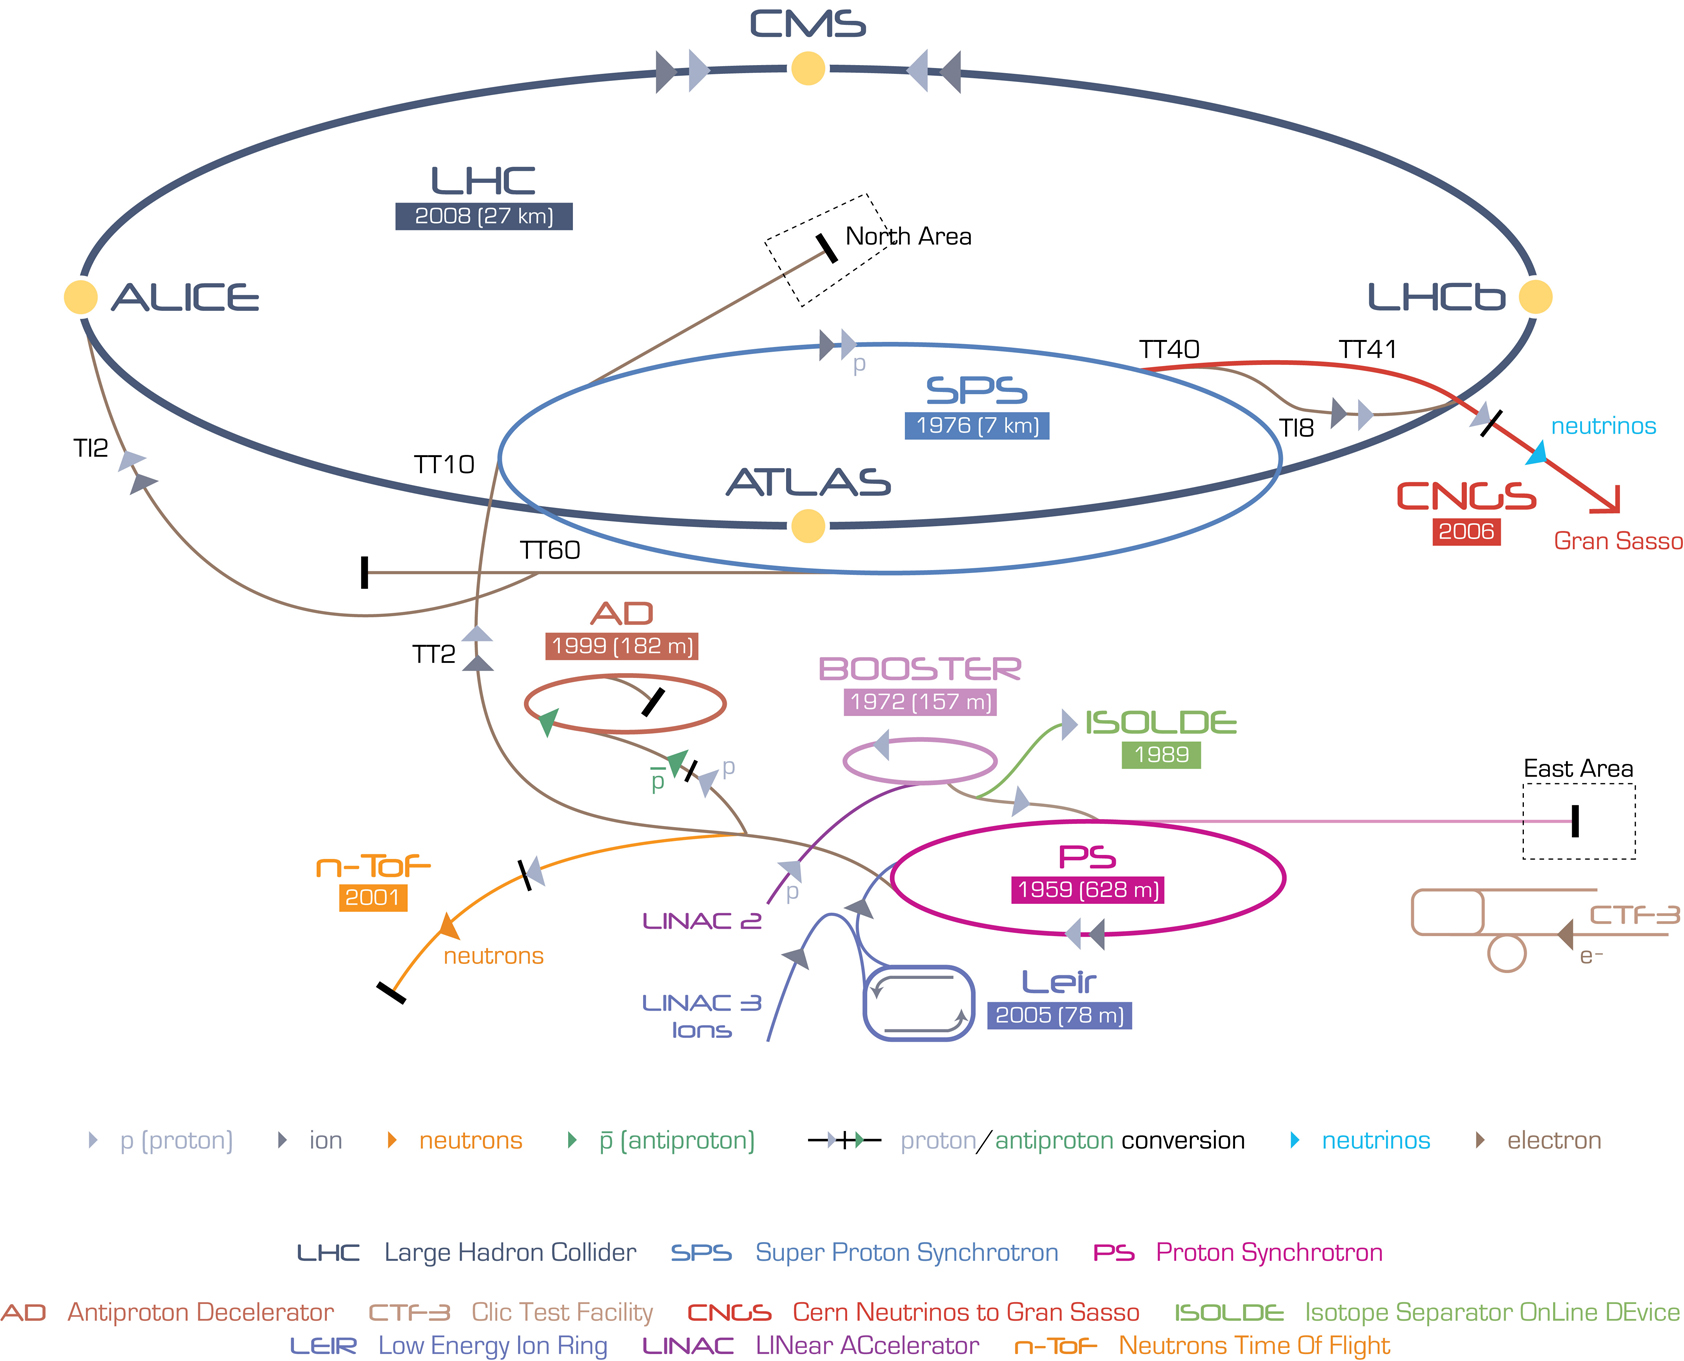
\includegraphics[width=0.8\textwidth]{figures/exp/accelerators.jpg}
\caption[The LHC accelerator complex]{The LHC accelerator complex, where the protons are accelerated by LINAC 2, the PS and the SPS before being injected into the main LHC ring, where they are collided in the 4 interaction points.}
\label{fig:lhc_accelerators}
\end{centering}
\end{figure}

\subsection{The accelerator complex}
In the main accelerator system consisting of two concentric counter-rotating rings, where superconducting magnets with a nominal B-field~$B=8.33~\mathrm{T}$~are used to bend and focus the beams, the protons are accelerated to the center-of-mass energy~$\sqrt{s} = 13$~TeV. Dipole magnets, depicted on~\cref{fig:lhc_magnet}, are used to bend the beam and multipole magnets for focusing. Both rings are located in beam pipes with an inner diameter of 48~mm within the same vacuum chamber in a so-called twin-bore design, dictated by the size of the tunnel. The magnets are kept at an operating temperature below 2K using liquid He-4. These proton bunches are collided at 4 interaction points and the beams can be sustained for up to 24~hours. The machine is characterized by the designed instantaneous luminosity of~$L=10^{34}~\mathrm{cm}^{-2}\mathrm{s}^{-1}$, which has been exceeded in 2017 by a factor of 1.58.

\begin{figure}
\begin{centering}
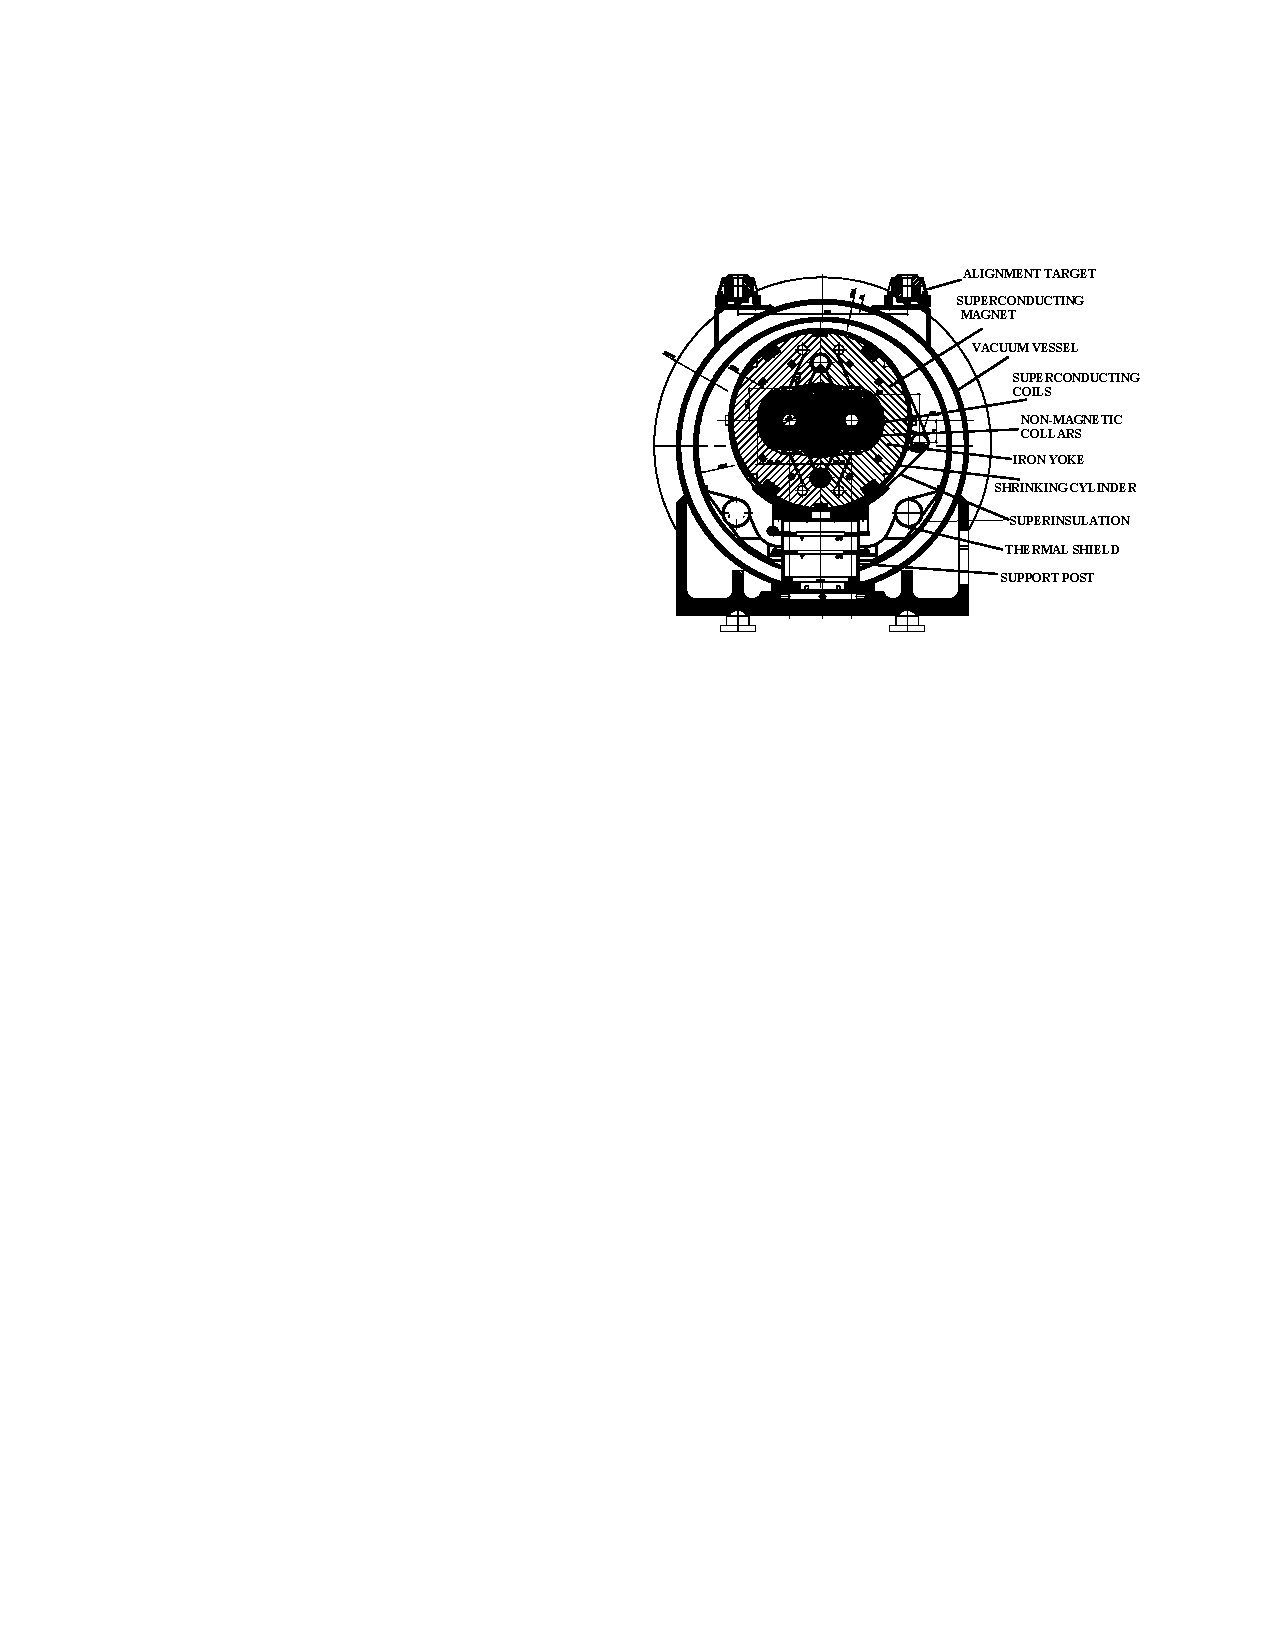
\includegraphics[width=0.8\textwidth]{figures/exp/cryodipole.pdf}
\caption{Cross-section of the LHC dipole magnet.}
\label{fig:lhc_magnet}
\end{centering}
\end{figure}

The proton-proton collisions at the LHC interaction points result in a number of events per second given by~$N_i = L \sigma_i$~for a process that has a cross-section~$\sigma_i$~at a given instantaneous luminosity~$L$. For the LHC, the machine luminosity is given by the Gaussian beam profile through

\begin{equation}
L = \frac{N_b^2 n_b f_\mathrm{rev} \gamma_r}{4 \pi \epsilon_n \beta^*} F
\end{equation}
where~$f_{\mathrm{rev}}$~is the number of revolutions per second and~$\gamma_r$~is the relativistic Lorentz factor. The beam is further described by the normalized transverse emittance~$\epsilon_n$~and the beta function~$\beta^*$~of the beam at the interaction point, which are related to the transverse beam size at a location~$s$~along the beam through~$\sigma(s) = \sqrt{\epsilon_n \beta(s)}$. The transverse emittance characterizes the spread of particles in the position-momentum phase space throughout their orbits. The beams cross at an angle~$\theta_c$, which results in the luminosity reduction factor

\begin{equation}
F = \biggl[1 + \bigr( \frac{\theta_c \sigma_z}{2 \sigma^*} \bigr)^2 \biggr]^{-1/2}
\end{equation}
where~$\sigma_z$~is the bunch length and~$\sigma^*$~the transverse bunch size. The~$\beta^*$~parameter dictates the size of the beam at the interaction point, which is tuned to the luminosity requirements of the experiment and in turn limited by the aperture of the focusing magnets. The maximum beam size in the transverse direction is~$\sigma=1.2~\mathrm{mm}$, limited by the dimensions of the beam screen. The instantaneous luminosity decays over time during a physics run due to beam loss from the collisions, such that the luminosity decreases by~$1/e$~during approximately~$15\ h$.

The total number of collisions in a given unit of time is characterized by the integrated luminosity~$\mathcal{L} = \int L\ \mathrm{d}t$~and is limited to around~$80-120~\mathrm{fb}^{-1}$~per year under perfect conditions, assuming around 200 days of operation and on average 7 hours of turn-around time between runs for filling the beams and accelerating to data-taking energies.

During the 2016 data taking period considered in this thesis, the LHC operated at a center-of-mass energy of~$\sqrt{s} = 13~\mathrm{TeV}$,~$\beta^* = 40~\mathrm{cm}$~and delivered around~$\mathcal{L} = 40~\mathrm{fb}^{-1}$~of proton-proton data to the ATLAS and CMS experiments. With an inelastic pp cross-section of~$\sigma_{pp} \simeq 77$~mb~\cite{VanHaevermaet:2016gnh}, this correspond to about~$10^{15}$~pp interactions.

\subsection{Experiments at the LHC}
The collision data form the LHC is recorded by 2 general purpose detectors, CMS and ATLAS (A Toroidal LHC ApparatuS), and 2 experiments with a more specialized physics program, LHCb and ALICE (A Large Ion Collider Experiment), located at the 4 interaction points. Overall, the general properties and physics goals of the experiment are as follows:

\begin{itemize}
    \item \textbf{CMS}: The main characteristic of CMS is the superconducting solenoid, which provides a magnetic field of 3.8T that enables the momentum of charged particles to be measured with high accuracy. Inside the solenoid volume are silicon pixel and strip trackers, an electromagentic calorimeter (ECAL) comprised of~$\mathrm{PbWO}_4$~crystals and a brass-scintillator hadronic calorimeter (HCAL). Outside the solenoid volume is the steel return yoke for the magnetic field, which contains gas-ionization chambers used to measure muons. The CMS detector was designed to meet a dimuon, diphoton and dielectron mass resolution of~$1\%$~at 100~GeV~\cite{Chatrchyan:2008aa}.
    \item \textbf{ATLAS}: The overall layout of the ATLAS machine differs from CMS mainly with respect to the configuration of the magnetic fields, where a central superconducting solenoid with B=2T houses the semiconductor trackers, with the lead-liquid argon (LAr) electromagnetic calorimeter and the hadronic calorimeters outside the solenoid volume. The muon systems are embedded in an outer air-core toroidal system that minimizes multiple scattering.
    \item \textbf{LHCb}: The primary goal of the LHCb experiment is to study heavy flavour physics, in particular rare decays of beauty and charm hadrons and searching for indirect evidence for new physics in CP-violation, exploiting the large rate of B-meson production at the LHC. The LHCb detector is a single-arm spectrometer with a forward angular coverage of 10 to 250-300~mrad, featuring a beryllium beampipe that is highly transparent to particle fluxes and an accurate vertexing system. LHCb operates at an instantaneous luminosity that is two orders of magnitude lower than CMS and ATLAS in order to minimize multiple pp interactions per bunch crossing.
    \item \textbf{ALICE}: The ALICE detector is designed to study heavy ions, focusing on QCD measurements, in particular the study of strongly interacting matter at the high temperatures and densities achievable in nucleon-nucleon collisions. It features general-purpose detectors in the barrel, embedded in a solenoid and muon spectrometers in the forward direction. The ALICE detector is specifically optimized to study global event observables such as particle multiplicity and energy flow. 
\end{itemize}
Both the CMS and ATLAS experiments have the broad physics goal of discovering the Higgs boson, studying its properties and searching for any new resonances at high energies. The discovery of the Higgs boson was realized during Run I of the LHC, with both experiments reporting a significant excess in 2012 that is compatible with a SM Higgs boson~\cite{Aad:2012tfa,Chatrchyan:2012xdj}. In the following section, we will discuss the essential aspects of the CMS experiment in more detail.

\section{The CMS detector}
The coordinate system adopted by CMS is centered at the collision point, with the x-axis pointing inward towards the LHC ring, y-axis vertically upward and the z axis along the beamline towards east in the direction of the Jura mountains. The azimuthal angle~$\phi$~is measured from the x axis in the plane transverse to the beam. The polar angle is measured from the z-axis and it defines the pseudorapidity~$\eta = -\ln{\tan{\theta/2}}$. The CMS detector follows a layered design that encapsulates the interaction region completely in the azimuthal direction and provides good coverage in the polar direction. In order to achieve this, the detector is divided into a barrel component and two endcaps, as can be seen on~\cref{fig:cms_experiment}. A transverse slide of the experiment can be seen on~\cref{fig:cms_slice}, where the overall layout of the subdetectors is pictured. 

\begin{figure}
\begin{centering}
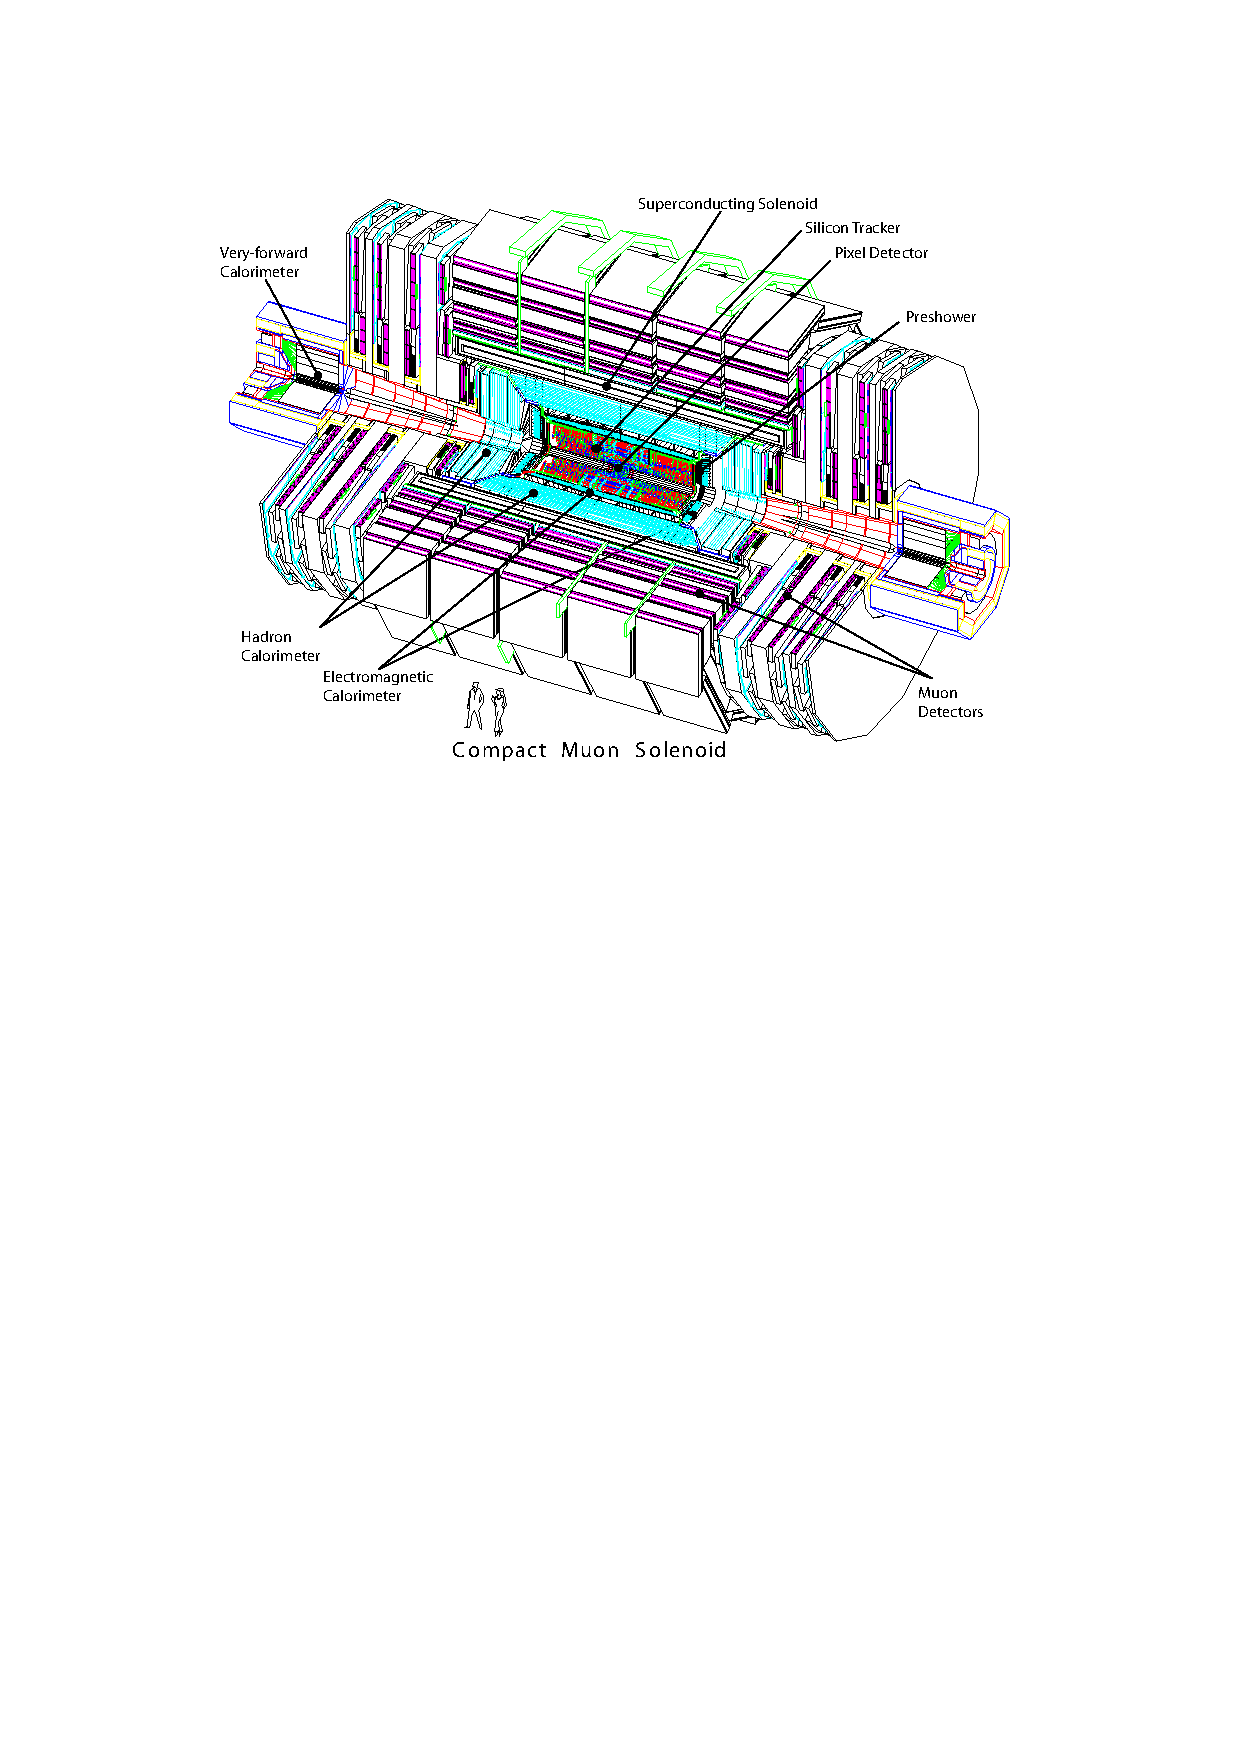
\includegraphics[width=0.8\textwidth]{figures/exp/cms.pdf}
\caption{The cross-section of the CMS experiment.}
\label{fig:cms_experiment}
\end{centering}
\end{figure}

\begin{figure}
\begin{centering}
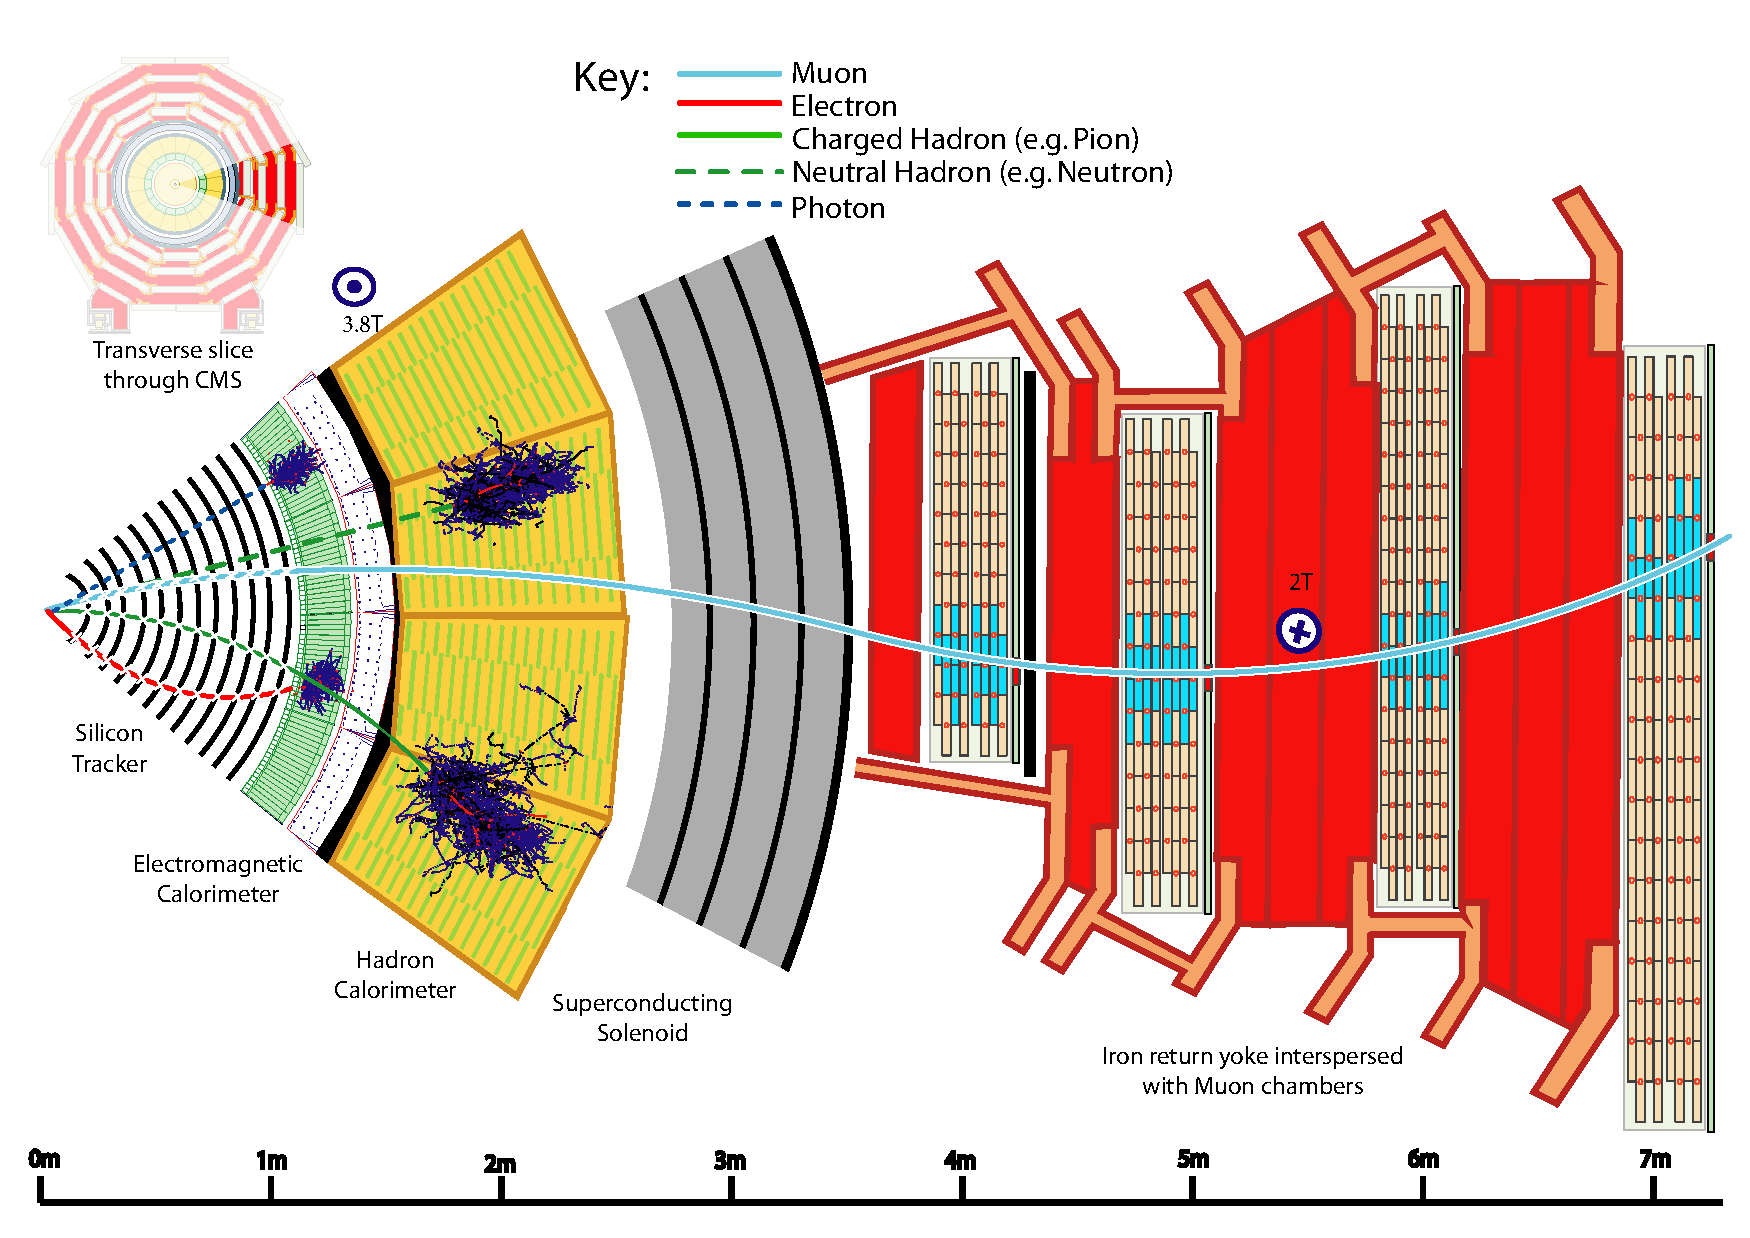
\includegraphics[width=0.8\textwidth]{figures/exp/cms_slice.pdf}
\caption{A view of a transverse slice of the CMS detector with the subsystems.}
\label{fig:cms_slice}
\end{centering}
\end{figure}

\subsection{The superconducting magnet}
The 3.8T magnetic field, which is essential for measuring the momenta and charge of charged particles, is created by the 220~ton superconducting solenoid, which has a diameter of 6~m and a length of 12.5~m. The energy stored in the NbTi conductor reaches up to 2.6~GJ, therefore the mechanical deformations in the magnet during energizing can be significant. The return yoke of the magnetic field consists of sections which house the muon chambers and thus guarantee a sufficient field strength in the muon spectrometer region.

\subsection{Inner tracking system}
The inner tracking system measures the momenta and trajectories of charged particles from the primary vertex in the interaction point and any secondary vertices associated to the decay of long-lived particles. The magnetic field is homogeneous within the tracker volume, which has a length of 5.8~m and a diameter of 2.5~m. The number of simultaneous inelastic collision (pileup) events per bunch crossing in pp collisions can be significant at the LHC, with nominal values around~$N_{PV} = 20$, but reaching an order of magnitude more in the HL-LHC. Therefore, the tracking system has to cope with high particle fluxes of up to~$10^3$~particles per bunch crossing every 25~ns and be able to associate signals to the correct bunch crossing. In order to keep the hit occupancy around 1\%, pixel detectors have to be used in the inner region of the tracker. The inner tracker consists of a 3-layer silicon pixel detector with layers at 4.4~cm, 7.3~cm and 10.2~cm and a silicon strip detector with 10 layers extending out to radii of 1.1~m. The pixels in the inner layer measure~$100\times150~\mathrm{\mu m}^2$~in the~$r-\phi$~and~$z$~directions, which is driven by the secondary vertex and impact parameter resolution necessary for the detection of heavy flavour states. The pixel detector covers the range range~$|\eta| < 2.5$~and consists of the barrel layers (BPix) and two endcap discs (FPix), located in such a way as to guarantee at least 3 pixel hits over almost the full range, as seen on~\cref{fig:cms_pixel}. By reading out the analog pulse height using charge sharing which results from the the B field, a hit resolution of 15-20~$\mathrm{\mu m}$~can be achieved. In total, the pixel detector covers an area of~$1~\mathrm{m}^2$~and consists of around 66 million pixels.

\begin{figure}
\begin{centering}
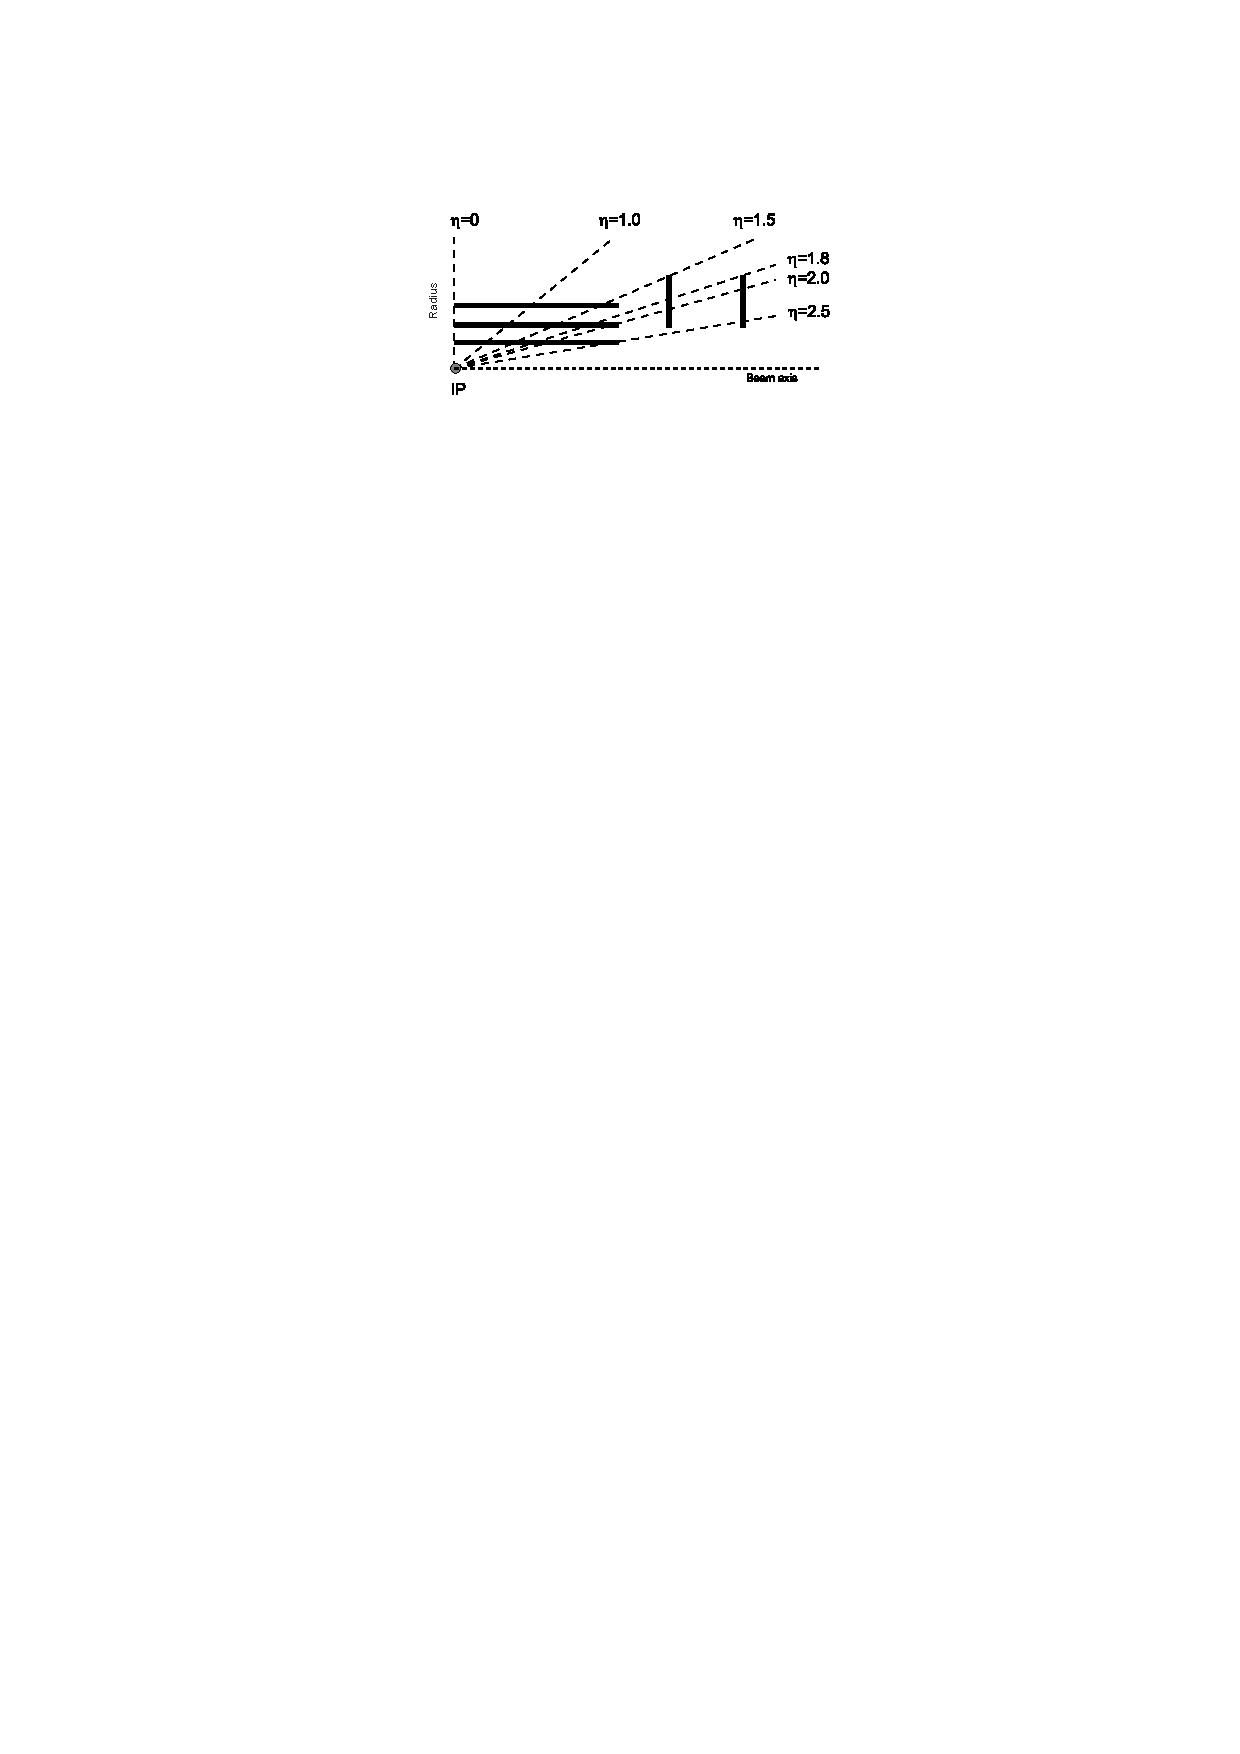
\includegraphics[width=0.6\textwidth]{figures/exp/pixel.pdf}
\caption{The schematic overview of the CMS pixel tracker.}
\label{fig:cms_pixel}
\end{centering}
\end{figure}

At larger radii, the occupancy decreases, such that silicon strips with a typical size of~$10\mathrm{cm} \times 80\mathrm{\mu m}$~are used in the silicon strip tracker. The tracker consists of several layered subsystems as shown on~\cref{fig:cms_tracker}, in particular, the tracker inner barrel and discs (TIB/TID), the outer barrel (TOB) and the tracker endcaps (TEC). The TIB/TID delivers 4 measurements of a track in the~$r-\phi$~direction, the TOB 6 measurements, and the TEC 9 measurements per particle trajectory. The strip pitch increases at larger radii to compensate for the reduction in particle flux.

\begin{figure}
\begin{centering}
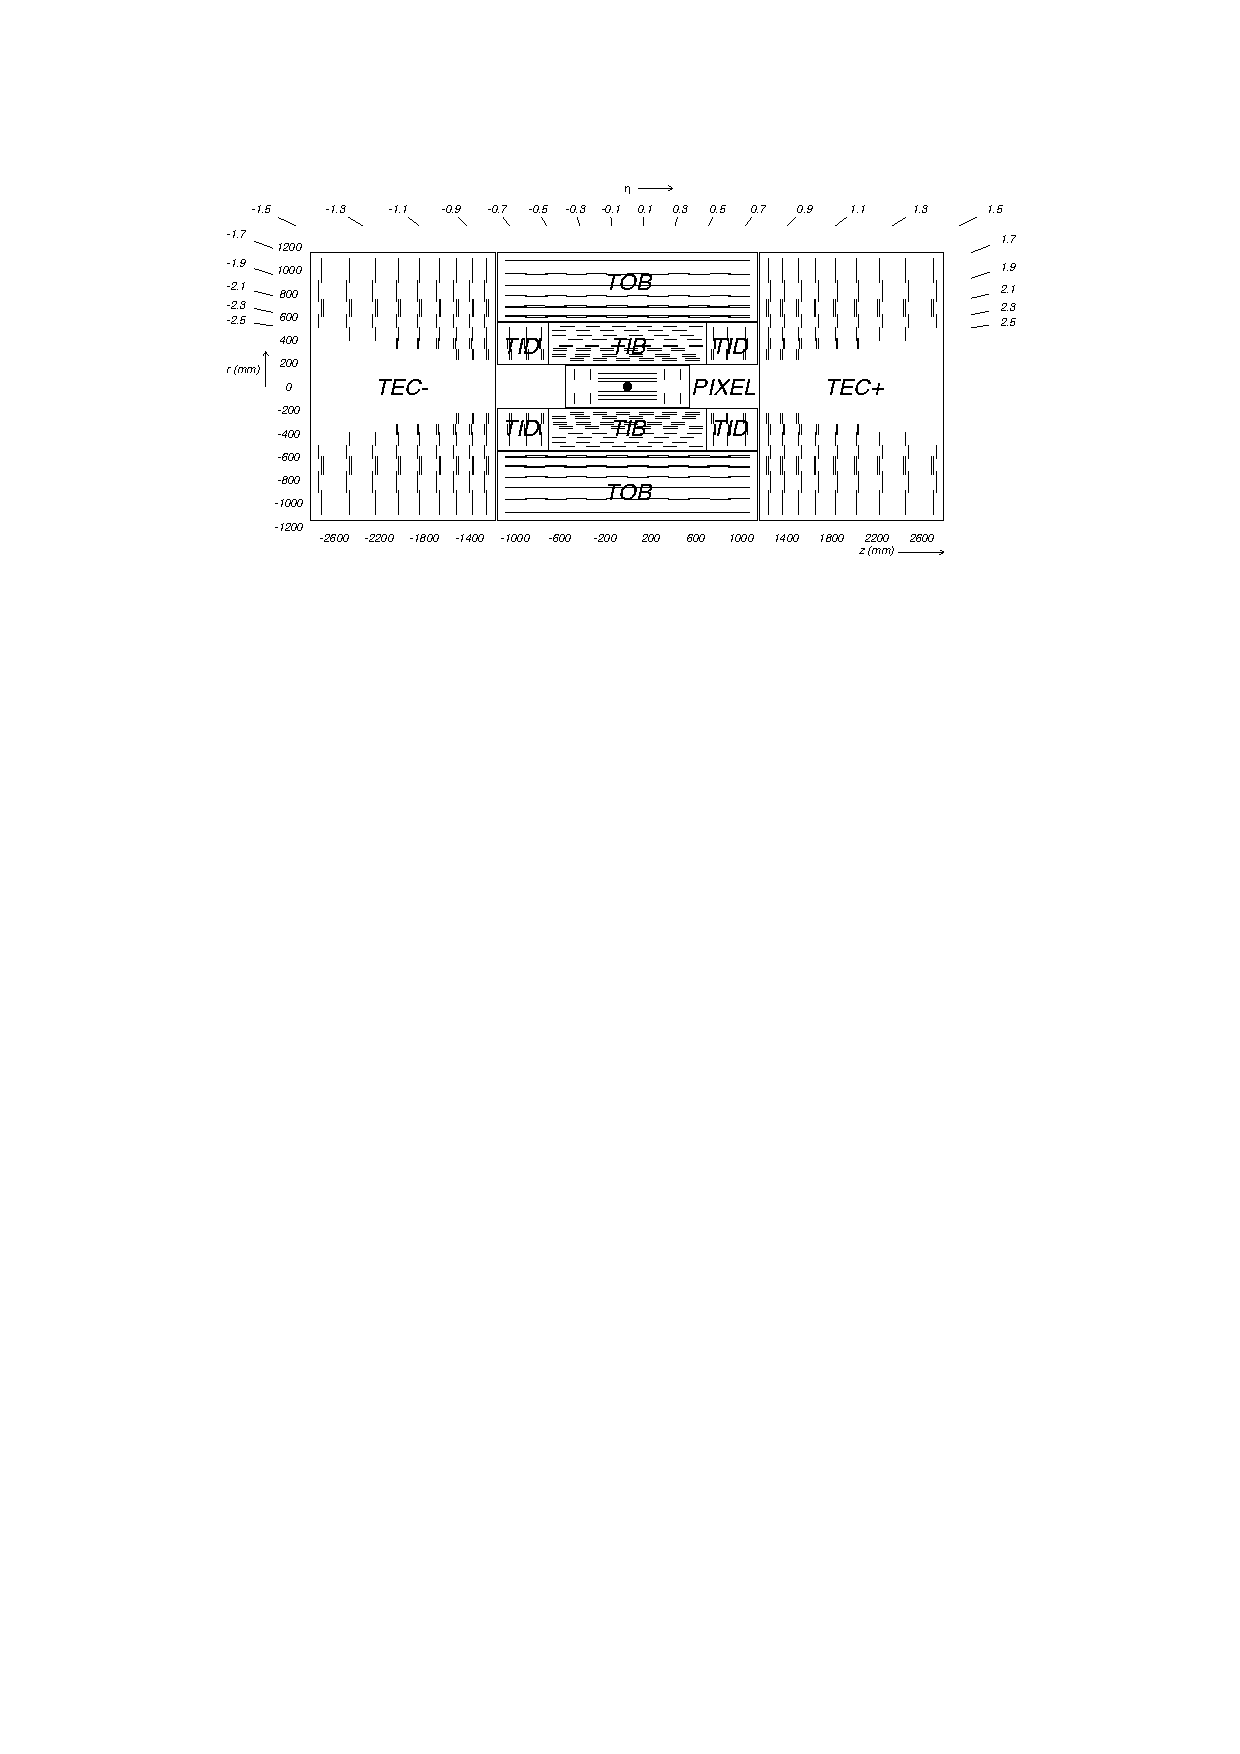
\includegraphics[width=0.6\textwidth]{figures/exp/tracker.pdf}
\caption[The CMS strip tracker]{The schematic overview of the CMS strip tracking system.}
\label{fig:cms_tracker}
\end{centering}
\end{figure}

Overall, the tracking system has to maximize the number of measurement points for each particle trajectory while keeping the material budget, measured in radiation lengths~$X_0$, at a minimum. Over the whole functional~$\eta$~range, the tracking system contributes between 0.4 and 1.8~$X_0$, with the largest radiation losses in the region around~$|\eta| \simeq 1.5$~due to the TIB/TID transition. Nevertheless, the transverse momentum resolution of muons is around~$1-2\%$~up to~$|\eta| \leq 1.6$, a reconstruction efficiency of around 99\% over most of the~$\eta$~range and of the transverse impact parameter resolution around~$10~\mathrm{\mu m}$~for high momentum tracks~\cite{Chatrchyan:2008aa}. 

The pixel detector was upgraded during the 2016-2017 winter shutdown procedure, adding an additional layer at~$r=2.9$~cm and improving the capabilities of the readout chip (ROC) to cope with an instantaneous luminosity of~$L = 2 \times 10^{34}\ \mathrm{cm}^{-2}\mathrm{s}^{-1}$~\cite{Tavolaro:2016hfj}.

\subsection{Electromagnetic calorimeter}
The primary function of the electromagnetic calorimeter is to measure the energy of electrons and photons through the production of scintillation light. The ECAL is situated within the solenoid volume in order to minimize energy losses from multiple scattering and consists of around 76000 lead-tungstenate~($\mathrm{PbWO}_4$) crystals arranged in the barrel and endcap, as seen on~\cref{fig:cms_ecal}. This material is characterized by a high density~($\rho = 8.28~\mathrm{g}/\mathrm{cm}^3$), a short radiation length ($X_0=0.89~\mathrm{cm}$) and a small Moliere radius~($R_M = 2.19~\mathrm{cm}$). Furthermore, the scintillation decay time is short, such that 80\% of the light is emitted during the 25~ns bunch spacing. The light is emitted with a broad maximum in the 420-430~nm range. In the barrel (endcaps), the crystals are coupled to avalanche photodiodes (vacuum phototriodes) for light collection, with a 1~MeV particle producing a yield of about 4.5 photoelectrons. Due to the high radiation damage expected throughout the lifetime of the ECAL, the light transmission properties of the crystals are monitored  using injected laser light at $\lambda = 440~\mathrm{nm}$. A two-layer lead absorber and silicon strip sensor preshower detector is located between the endcaps and the interaction point, covering $1.65 < |\eta| < 2.6$, in order to improve the discrimination between photons and $\pi^0$.

\begin{figure}
\begin{centering}
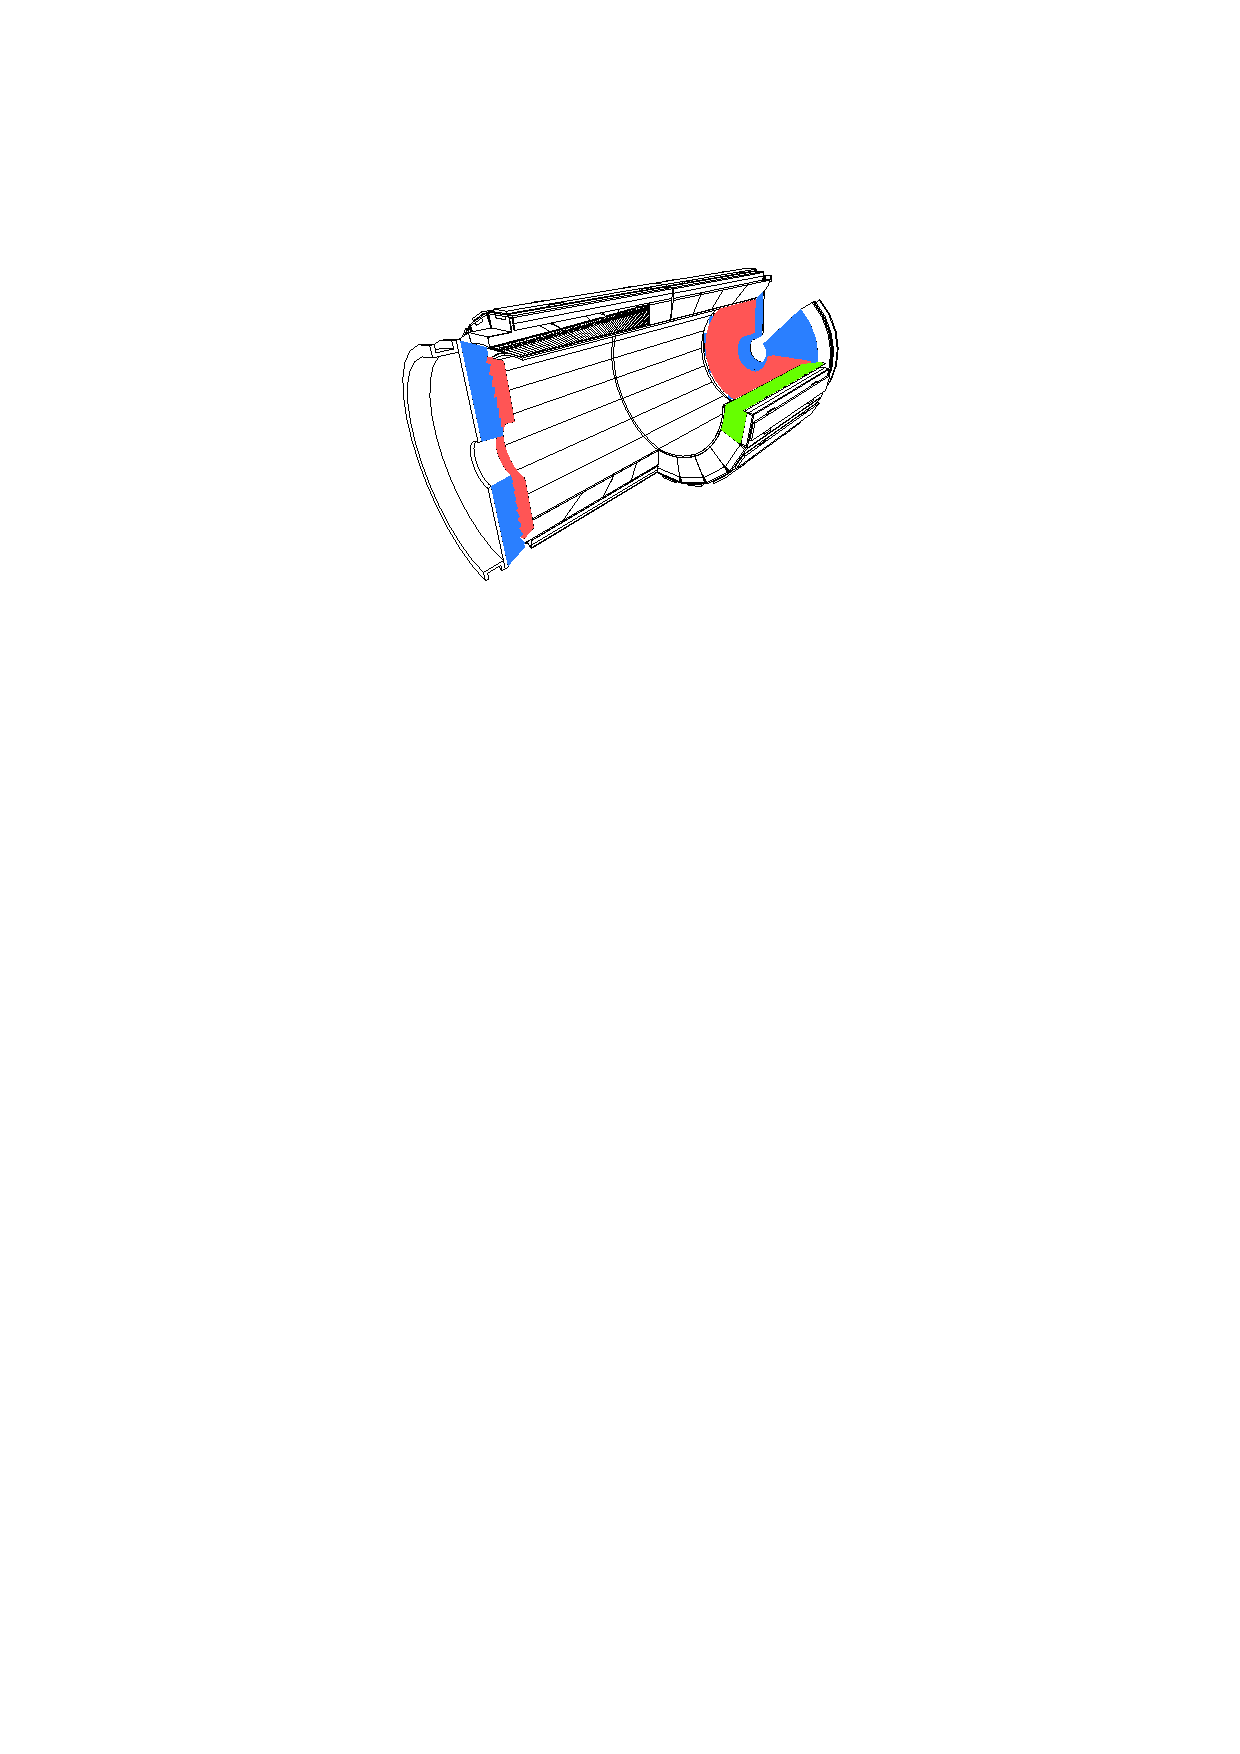
\includegraphics[width=0.6\textwidth]{figures/exp/ecal.pdf}
\caption[The structure of the CMS electromagnetic calorimeter]{The CMS electromagnetic calorimeter, with the barrel crystal clusters in green, the endcaps in blue and the preshower in red.}
\label{fig:cms_ecal}
\end{centering}
\end{figure}

The ECAL barrel region extends to~$|\eta| < 1.479$, with a 360-fold (190-fold) granularity in the azimuthal (polar) direction and the endcaps between~$1.479 < |\eta| < 3.0$. Since the photon emission in scintillation and subsequent amplification are temperature-dependent, the ECAL has to be maintained at a constant temperature within~$0.05\degree~\mathrm{C}$. In order to reconstruct the signal pulse from the photodetectors, a new technique is used in Run II, where the signal amplitude templates from up to 9 bunch crossings around the in-time signal are fitted to the observed 10-sample signal, in order to determine signal amplitude in the presence of both in-time and out-of-time pileup~\cite{Brianza:2017slq}. The energy resolution of the ECAL has been measured in electron test beams, arranging the crystals in a $3\times3$ matrix to minimize energy leakage, and found to be

\begin{equation}
\frac{\sigma_E}{E} = \frac{a}{\sqrt{E}} \oplus \frac{b}{E} \oplus c
\end{equation}
with $a = 2.8\%$ being the stochastic term, $b = 12\%$ the noise term and $c = 0.3\%$ the irreducible term from non-uniformities for the barrel~\cite{Adzic:2007mi}.

Since there is about $1-2X_0$ of material in front of the ECAL which results in significant multiple scattering and the crystals are about one Moliere radius in the lateral dimension, the energy from a single electromagnetic shower is spread over multiple crystals. In order to reconstruct the energy of incident particles, the energy that is spread over multiple ECAL crystals is clustered by merging crystals into superclusters. The ECAL has an excellent energy resolution, with photons from the decay of a 125-GeV Higgs boson being reconstructed in the barrel with an energy resolution between 1.1\% and 2.6\%~\cite{Chatrchyan:2013dga}.

\subsection{Hadronic calorimeter}
The purpose of the HCAL is to measure the energies of hadron jets and to have a hermetic energy coverage of the detector, such that the missing transverse energy resulting from neutrinos or hypothetical weakly interacting particles could be determined. The HCAL consists of a barrel and endcaps extending to $|\eta| < 3.0$, with a forward calorimeter covering the range up to $|\eta|<5.0$, as seen on~\cref{fig:hcal}.

\begin{figure}
\begin{centering}
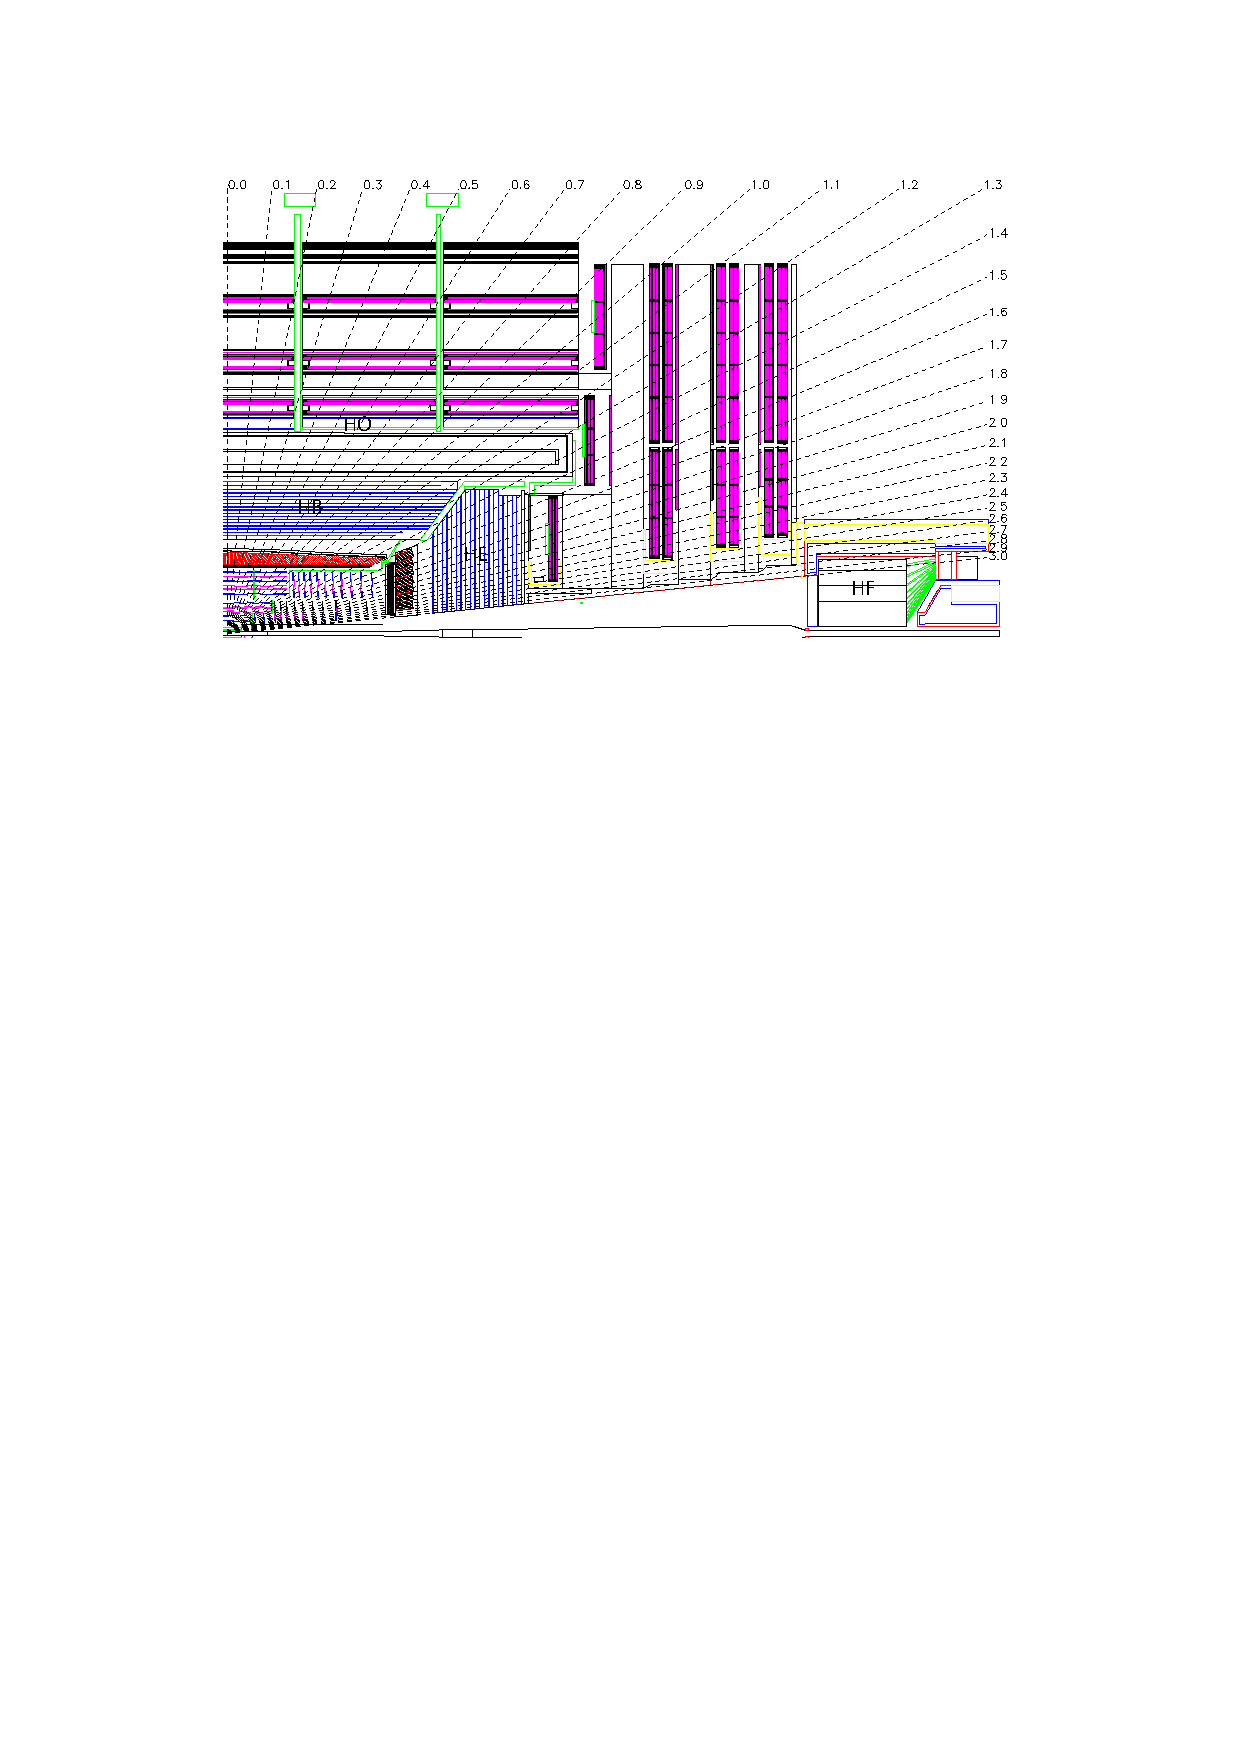
\includegraphics[width=0.6\textwidth]{figures/exp/hcal.pdf}
\caption[The cross-section of the CMS hadronic calorimeter]{The cross-section of the CMS hadronic calorimeter, showing the barrel region (HB), the endcap (HB), the outer calorimeter (HO) and the forward calorimeter (HF).}
\label{fig:hcal}
\end{centering}
\end{figure}


The HCAL barrel is situated between the ECAL and the superconducting coil in the region~$1.77~\mathrm{m} < R < 2.95~\mathrm{m}$. As this limits the amount of material, an outer hadron calorimeter is installed outside the solenoid in the barrel region, such that the material amounts to around 11 hadronic radiation lengths. The HCAL barrel regions extends to $|\eta| < 1.3$ and consists of an absorber made from brass sandwiched between steel plates with embedded scintillator tiles. The scintillation light is read out by bringing the light to photodiodes in readout towers using wavelength shifting fibres. Hybrid photodiodes are used due to their low sensitivity to the magnetic field and a large dynamical range.

The HCAL endcaps cover the pseudorapidity range $1.3 < |\eta| < 3$, thus they need to handle high counting rates and be radiation hard. They follow a similar construction as the barrel, with an absorber/scintillator design with a segmentation granularity of~$\Delta \eta \times \Delta \phi = 0.087 \times 0.087$~for~$|\eta| < 1.6$~and~$\Delta \eta \times \Delta \phi \simeq 0.17 \times 0.17$ for the rest of the endcap.

The forward calorimeter (HF) located at $\pm$11 m from the interaction point, covering the range $3.0 < |\eta| < 5.2$, is situated in an extreme radiation environment of up to 100 Mrad/year, thus radiation hardness has been the primary design criterion. It is based on the collection of Cherenkov light collected in quartz fibres embedded in steel absorber plates, read out by photomultiplier tubes. The HF is mostly sensitive to the electromagnetic component of showers~\cite{Akchurin:2003tp}. The HF can be used for luminosity monitoring in CMS to infer the mean number of interactions per bunch crossing and thus an accurate determination of the normalization for physics analyses.

The energy resolution of the HCAL has been determined in test beams using single pions and found to be approximately~$\sigma/E = 110\%/\sqrt{E} \oplus 9\%$~\cite{Elvira:2004iya} with a typical readout noise of 200~MeV per tower. The particle flow algorithm is further used to build a global representation of the event based on the detector signals from other subsystems~\cite{CMS-PRF-14-001}.

\subsection{The muon systems}
Muon detection is of central importance to CMS, as they can be detected relatively easily and are produced in several interesting decays, such at $\mathrm{H} \rightarrow \mathrm{Z} \mathrm{Z}^* \rightarrow 4 \mathrm{\mu}$. The muon systems in CMS are used to identify muons over a wide angular range up to $|\eta| < 2.4$, to measure their charge and momentum and for triggering purposes. The punch-through of other particles to the muon systems is negligible due to the amount of material, which is around 16$X_0$. The muon efficiency is around 95-99\% and the $p_T$-resolution between 15\% in the barrel and 25\% in the endcap, which is necessary to use the muon system for triggering. Since the muon systems cover a large area around the detector in the form of a barrel and endcaps, they have to be inexpensive and robust.

In the barrel region, drift tubes that are organized into 4 stations arranged in concentric cylinders within the return yoke. The drift tubes use a mixture of~$\mathrm{Ar}/\mathrm{CO}_2$~gas and each chamber consists of 4 layers arranged into a superlayer. This provides a timing resolution of a few nanoseconds and allows the muon system readout to be assigned to a bunch crossing. The spatial resolution of the drift chambers has been measured in test beams to be around~$300~\mathrm{\mu m}$, determined by the dispersion of the drift time and distortions of the drift caused by magnetic fields. The bunch crossing identification efficiency, which is important for triggering, is better than 90\%, driven by the timing resolution and muons producing electromagnetic showers.

In the endcaps, the muon system consists of cathode strip chambers (CSC), which have the advantage that they can operate at the high rates and non-uniform magnetic field present in the forward region. The spatial resolution of a hit is around~$\sim 80~\mathrm{\mu m}$~in the combined 6-plane CSC chamber and the bunch tagging efficiency is around 98-99\%.

In order to complement the time resolution of the drift tubes and the CSC, a trigger system based on resistive place chambers (RPC) exists in the barrel and endcaps. The RPC operates on the principle of an avalanche generated in a gas gap between two resin plates, such that the bunch crossing assignment can be done with rates up to~$1~\mathrm{kHz}/\mathrm{cm}^2$. The timing resolution of a few nanoseconds provided by the RPC crucially improves the trigger efficiency.

Since manufacturing tolerances, the intense magnetic field and thermal stress can cause the geometry of the muon system to change at the level of up to a few centimeters, it is monitored using an optical alignment system. 

\subsection{Trigger, data acquisition and computing}
The data from the 40~MHz LHC collisions needs to be reduced by a factor of $10^6$ for storage and analysis. This means that some form of triggering needs to be applied in order to select the most interesting physics events containing high-energy particles. The CMS experiment employs a 2-level trigger system, where the Level-1 (L1) trigger is implemented in custom programmable electronics and operates on the level of the calorimeters and the muon systems, whereas the high-level trigger (HLT) has access to the complete event read-out and is implemented on a conventional CPU farm.

The L1 trigger is composed of the trigger primitive generators, which operate on the level of calorimeter trigger towers, track segments and hit patterns on muon chambers.  This information is combined using regional triggers to determine trigger objects in limited spatial regions of the detector. These objects are then compared by the global calorimeter and muon triggers, which determine if sufficient good-quality muon or calorimeter objects are present to accept the event. The processing is pipelined such that the deadtime is minimized.

The global calorimeter trigger works on the basis of jets, total transverse energy, missing transverse energy and $H_T$, the scalar transverse energy sum of jets. Furthermore, it provides isolated and non-isolated $\mathrm{e}/\mathrm{\gamma}$ candidates. The muon system trigger works on the basis of reconstructing track candidates from hits in the drift tubes, the CSCs and the RPCs. In the global muon trigger, the muon candidates are identified by $p_T$, charge, $\eta$, $\phi$ and quality parameters, as well as isolation information from the global calorimeter trigger.

The maximal output rate of 100~kHz of the L1 trigger is fed into the HLT, which further reduces the recorded events to a rate of about 100~Hz. The data are divided to luminosity sections of~$2^{20}$~LHC orbits~(93~s), during which trigger thresholds and trigger prescale factors, which sample the trigger acceptance, are not changed. The total amount of zero-suppressed data recorded for a bunch crossing is of the order of 1~MB.

If an event is accepted by the HLT, it is transferred to the CMS offline computing infrastructure, which consists of several computing tiers with the bulk of the computing resource located in centers around the globe. The Tier 0 center at CERN performs the prompt reconstruction of the data and transfers it to several Tier 1 centers for storage, where late-stage reconstruction with improved calibrations can take place. Data analysis and MC simulation happens primarily at Tier 2 centers, which are associated to Tier 1 sites and divide the resources between the CMS collaboration and the local physics community. A typical Tier 2 site hosts 1-2~PB of data and O(5000) CPUs.

%\chapter{Identification of jets from bottom quarks}
Accurately identifying jets from bottom quarks is a crucial part of physics program involving top quarks, which decays before hadronization to b quarks and the W boson, and the Higgs boson, which decays primarily to b quarks. This amounts to measuring the quantum numbers of the partons that give rise to individual jets.

The relatively large lifetime, the hadronization properties of the bottom quark and the possible semileptonic decays of b~hadrons allow us to experimentally identify the jets that arise from bottom and charm quarks through the technique of b tagging, or more generally flavour tagging. A b quark has a relatively long lifetime of $10^{-12}$ seconds and a large Lorentz boost factor, resulting in hadronization at a decay vertex that is displaced by several millimetres with respect to the primary interaction point.

The idea of b tagging is to use a combination of discriminating variables to distinguish between jets from bottom, charm and light quarks on a statistical basis by assigning a discriminator value for jets that is on average higher for jets arising from bottom quarks than for the ones arising from light quarks. Jets that pass a certain pre-determined threshold of the discriminator value are taken to be tagged as a certain flavour. This technique based on the presence of a secondary vertex was first used at Tevatron in the analyses that led to the discovery of the top quark~\cite{Abe:1994st,Abe:1995hr}.

In this chapter, we will give an overview of b tagging at CMS, with a specific focus on the development and re-optimisation of the Combined Multivariate~(cMVAv2) b~tagging algorithm for Run II. We start with an overview of the discriminating variables important for b~tagging, followed by a description of the existing b~tagging algorithms at CMS. We then introduce the cMVAv2 algorithm and describe the optimisation and performance of the retrained version in Run II. We conclude with an outlook on flavour tagging. 

\section{Discriminating variables}
The most important discriminating variables for flavour tagging are the kinematic properties of jets and the associated leptons, as well as the existence and properties of tracks from charged particles and vertices associated to either the primary hard interaction in the proton-proton collision or the secondary vertices from the decay of b or c~hadrons. The secondary vertex of b~hadron decay, which is displaced with respect to the primary vertex due to the long life time of b~hadrons, is an especially salient feature of b~hadron decays that the b~tagging algorithms seek to exploit through accurate track and vertex reconstruction. Therefore, the selection of good tracks and the reconstruction of secondary vertices is necessary for efficient b~tagging.

\subsection{Track selection}
The tracks reconstructed by the inner tracking detector and associated to jets are used for b~tagging only in case they are of sufficient quality, i.e. they pass the track selection. This means they must have a transverse momentum of at least~1~GeV, a normalized~$\chi^2$~quality parameter for the fit to hits below~5 and at least~8 hits in the tracker with at least 2 in the inner pixel detector. Furthermore, the impact parameter~(IP), shown on \cref{fig:btag_ip}, is defined as the distance of closest approach between the primary vertex and the track trajectory is required to be less than~0.2~(17)~cm in the transverse~(longitudinal) direction to ensure that the tracks are sufficiently close to the primary vertex and thus reduce the contribution from pileup. The distance of closest approach between the jet and the track must be smaller than~0.07~cm and the decay length, defined as the distance between the primary vertex and the point of closest approach between the track and the jet must be less than~5~cm. Jets at $p_T = 100~\mathrm{GeV}$~are estimated to have around 7 associated tracks, with the multiplicity rising significantly at higher momenta. \cite{CMS-PAS-BTV-15-001}.

\begin{figure}
\begin{centering}
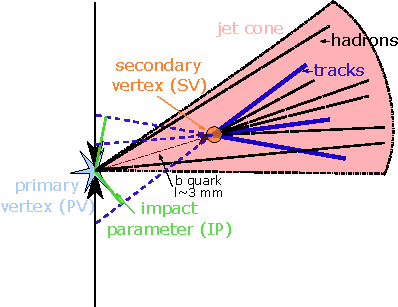
\includegraphics[width=0.4\textwidth]{figures/btv/ip.pdf}
\caption[Illustration of b~quark decay]{An illustration of the decay of a b~quark, along with the definition of the secondary vertex and the impact parameter.}
\label{fig:btag_ip}
\end{centering}
\end{figure}


\subsection{Vertex reconstruction}
Tracks passing the pileup-suppressing selection selection are used for vertex reconstruction in the adaptive vertex reconstruction~(AVR) algorithm~\cite{Waltenberger:2008zz}. Vertices reconstructed by AVR must pass further selection criteria designed to suppress vertices that are unlikely to originate from b~hadron decay. These selection criteria require a vertex to have a sufficient number unique tracks, a high-significance flight distance, a mass of less than~6.5~GeV and incompatible with the~$K_S^0$~hadron. Upon fulfilling these criteria, a jet is assigned to contain an AVR vertex~\cite{CMS-PAS-BTV-15-001}.

An alternative to AVR, where tracks are required to be associated to jets and therefore vertex reconstruction is seeded by jets, is the inclusive vertex finder~(IVF) algorithm~\cite{Khachatryan:2011wq}. As the name implies, the IVF algorithm starts with the set of all tracks in the event that pass somewhat looser selection criteria than used for AVR. Vertices are found by fitting all tracks simultaneously using an adaptive fitting algorithm looking for clusters of tracks. A further arbitration step assigns tracks to either the primary or secondary vertex based on compatibility and pixel hits, or removes secondary vertices of low quality. The IVF algorithm reconstructs about~10~\%~(15~\%)~more often the vertices from bottom~(charm) hadrons, but also increases the fraction of vertices reconstructed for light jets by about~8~\%. The overlap between the two algorithms is about~60\%, meaning that both vertex fitters provide some independent information on the event~\cite{CMS-PAS-BTV-15-001}.

\section{Multivariate b~taggers}
Using machine learning, signals from various regions of the detector can be combined effectively to develop a discriminator between b jets and light jets. Such techniques are especially suited to exploit sources of information that are partially correlated, such as the AVR and IVF vertices. The cMVAv2 b~tagging algorithm combines the output of different low and high level b~tagging algorithms, developed independently and using partially correlated variables, into a single high level discriminator. Before we can describe the cMVAv2 in detail, we must therefore discuss the different b~tagging algorithms used at CMS.

\subsubsection{Jet probability taggers}
The Jet Probability (JP) tagger was developed during Run I and is a simple multivariate likelihood discriminator based on track properties. In JP, the likelihood for a jet to originate from the primary vertex, as opposed to a secondary vertex, is computed by multiplying the per-track likelihoods, based on the track impact parameter and detector resolution. In a version of the JP tagger, the 4 tracks that have the highest IP significance~($\mathrm{IP} / \sigma_{\mathrm{IP}}$) are given a higher weight such that the new tagger, denoted Jet B-Probability (JBP) is more efficient in discriminating against b jets~\cite{Chatrchyan:2012jua}. The discriminator distributions for the JP and JBP b~taggers are shown on~\cref{fig:btag_jbp}.

\begin{figure}
\begin{centering}
\subfloat[The JP b~tagger]{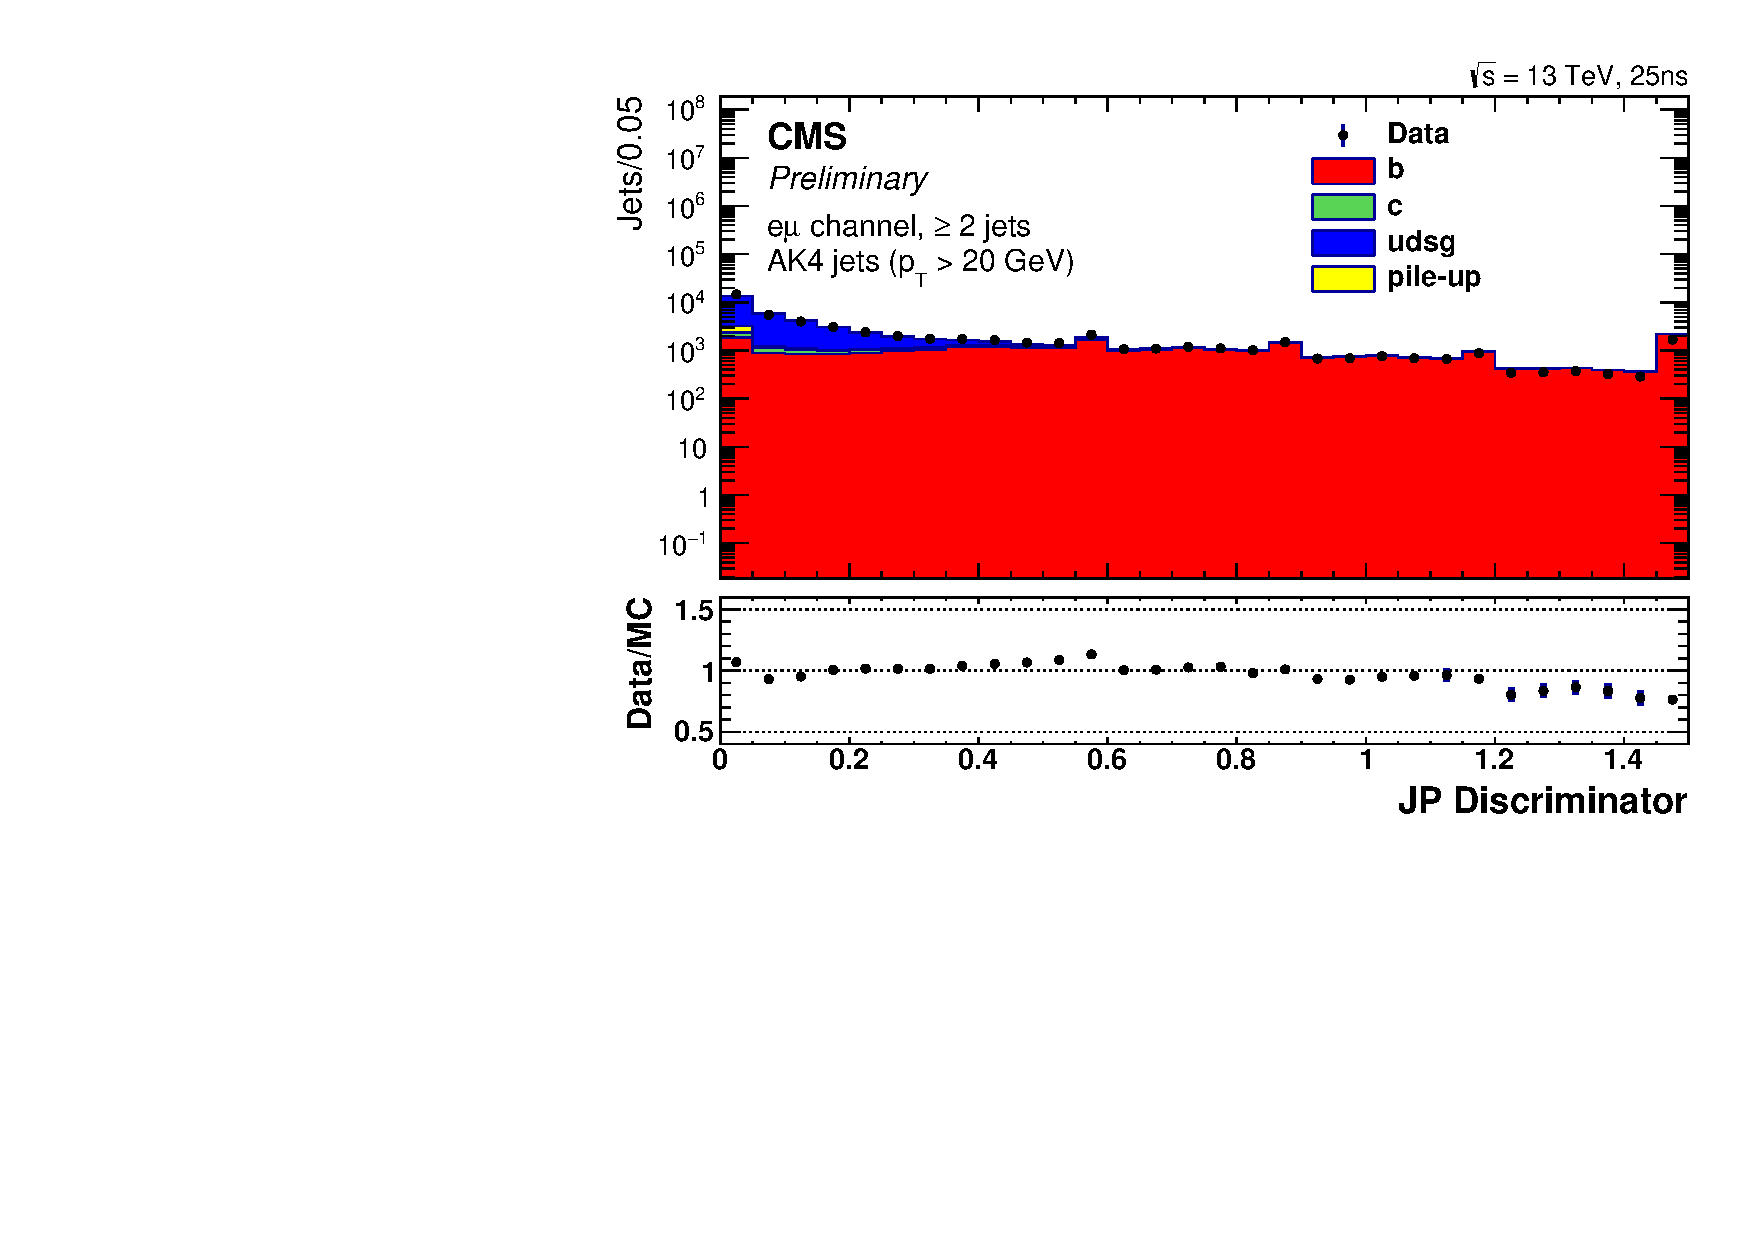
\includegraphics[width=0.5\textwidth]{figures/btv/jp.pdf}}
\subfloat[The JBP b~tagger]{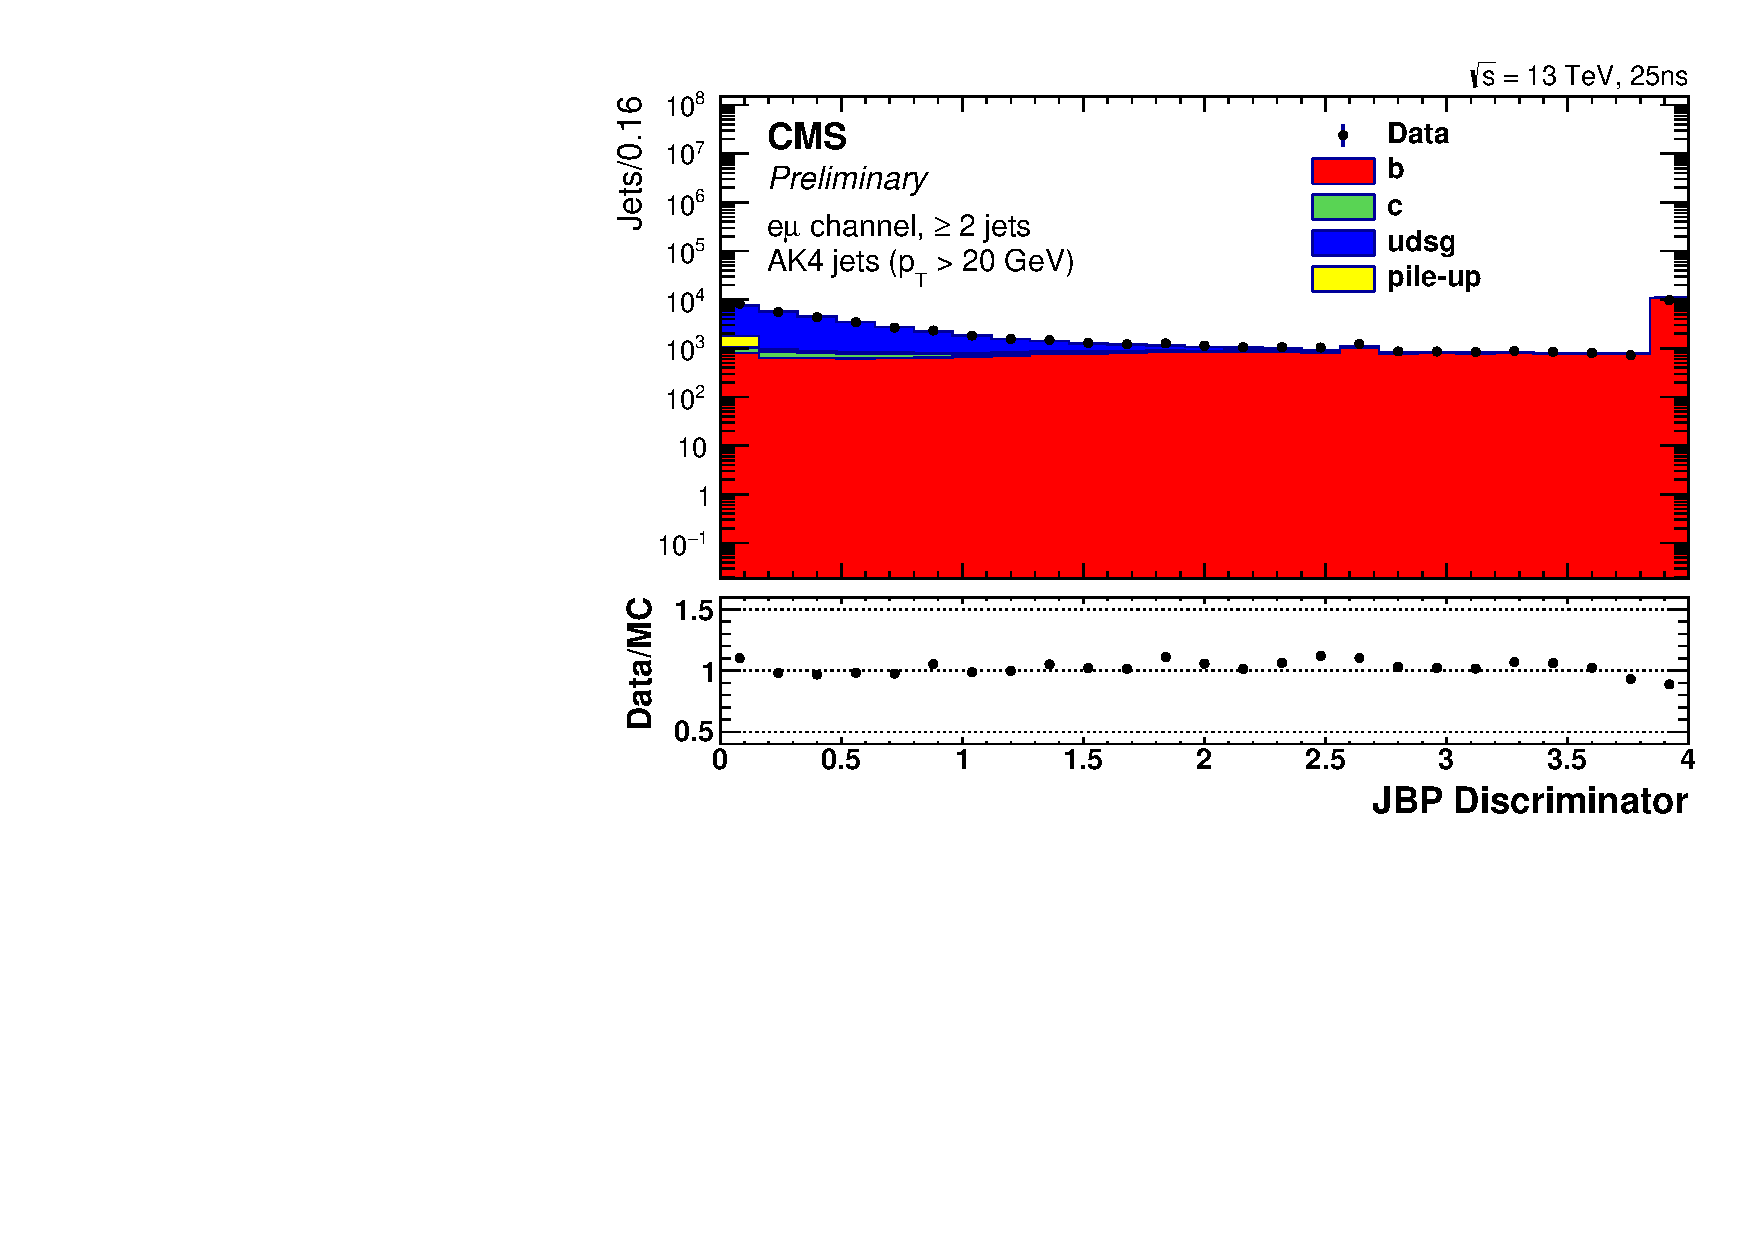
\includegraphics[width=0.5\textwidth]{figures/btv/jbp.pdf}} \\
\caption[The jet probability b discriminator distributions]{The jet probability b taggers in dileptonic ($\mathrm{e\mu}$) \ttbar+jets events. Figures from~\cite{CMS-PAS-BTV-15-001}.}
\label{fig:btag_jbp}
\end{centering}
\end{figure}

\subsubsection{Soft lepton taggers}
The semileptonic decays of the b~hadron to muons through~$\mathrm{b} \rightarrow \mathrm{\mu}^- \bar{\nu}_{\mathrm{\mu}} s$, which happens with a branching fraction of about~$20\%$, makes it possible to use the presence of a reconstructed muon in a jet for b~tagging. The Soft Muon (SM) algorithm in CMS relies on the presence of a muon in the jet constituents, but not on the presence of a secondary vertex. Similarly, the decay of a b~hadron to an electron is exploited through the Soft Electron (SE) tagger~\cite{CMS-PAS-BTV-15-001}. The discriminator distributions are shown on~\cref{fig:btag_softlep}.

\begin{figure}
\begin{centering}
\subfloat[The soft electron b~tagger]{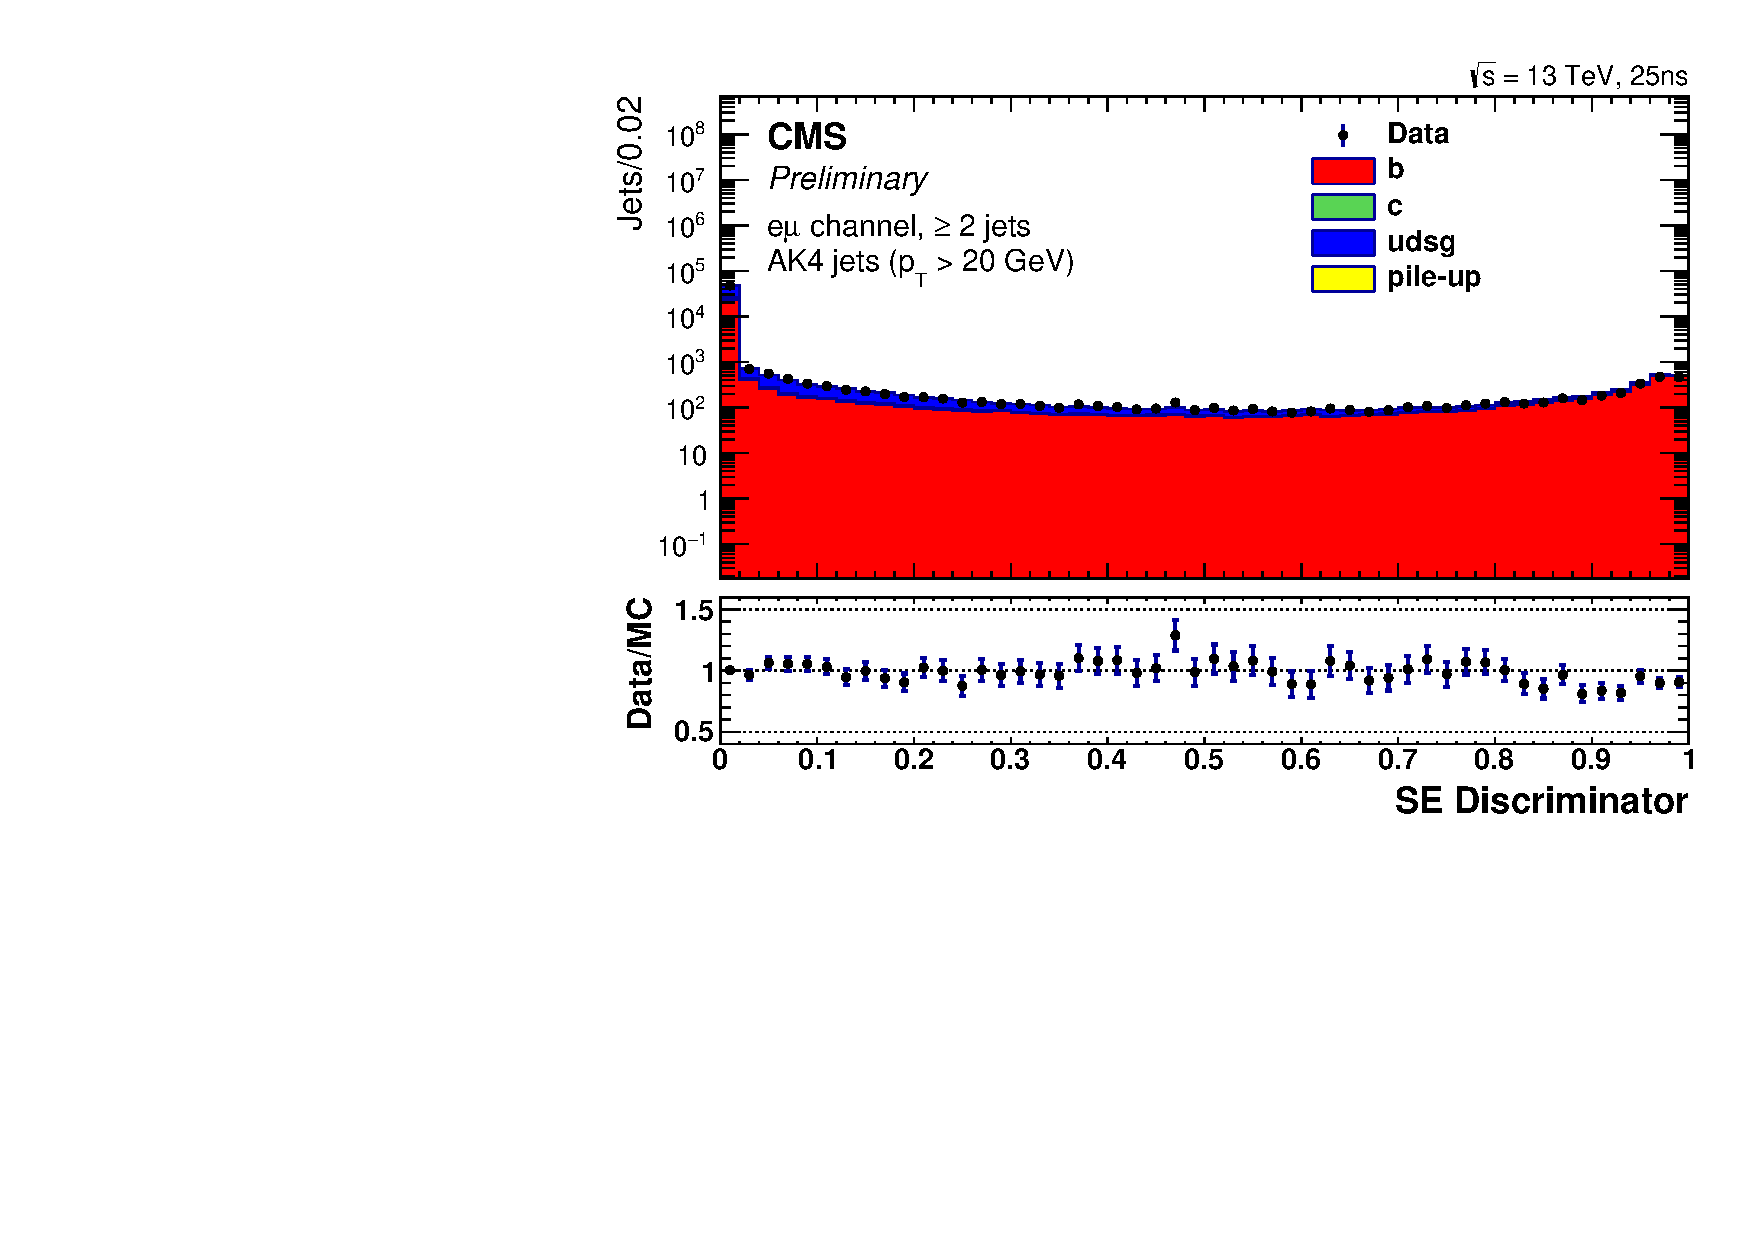
\includegraphics[width=0.5\textwidth]{figures/btv/softel.pdf}}
\subfloat[The soft muon b~tagger]{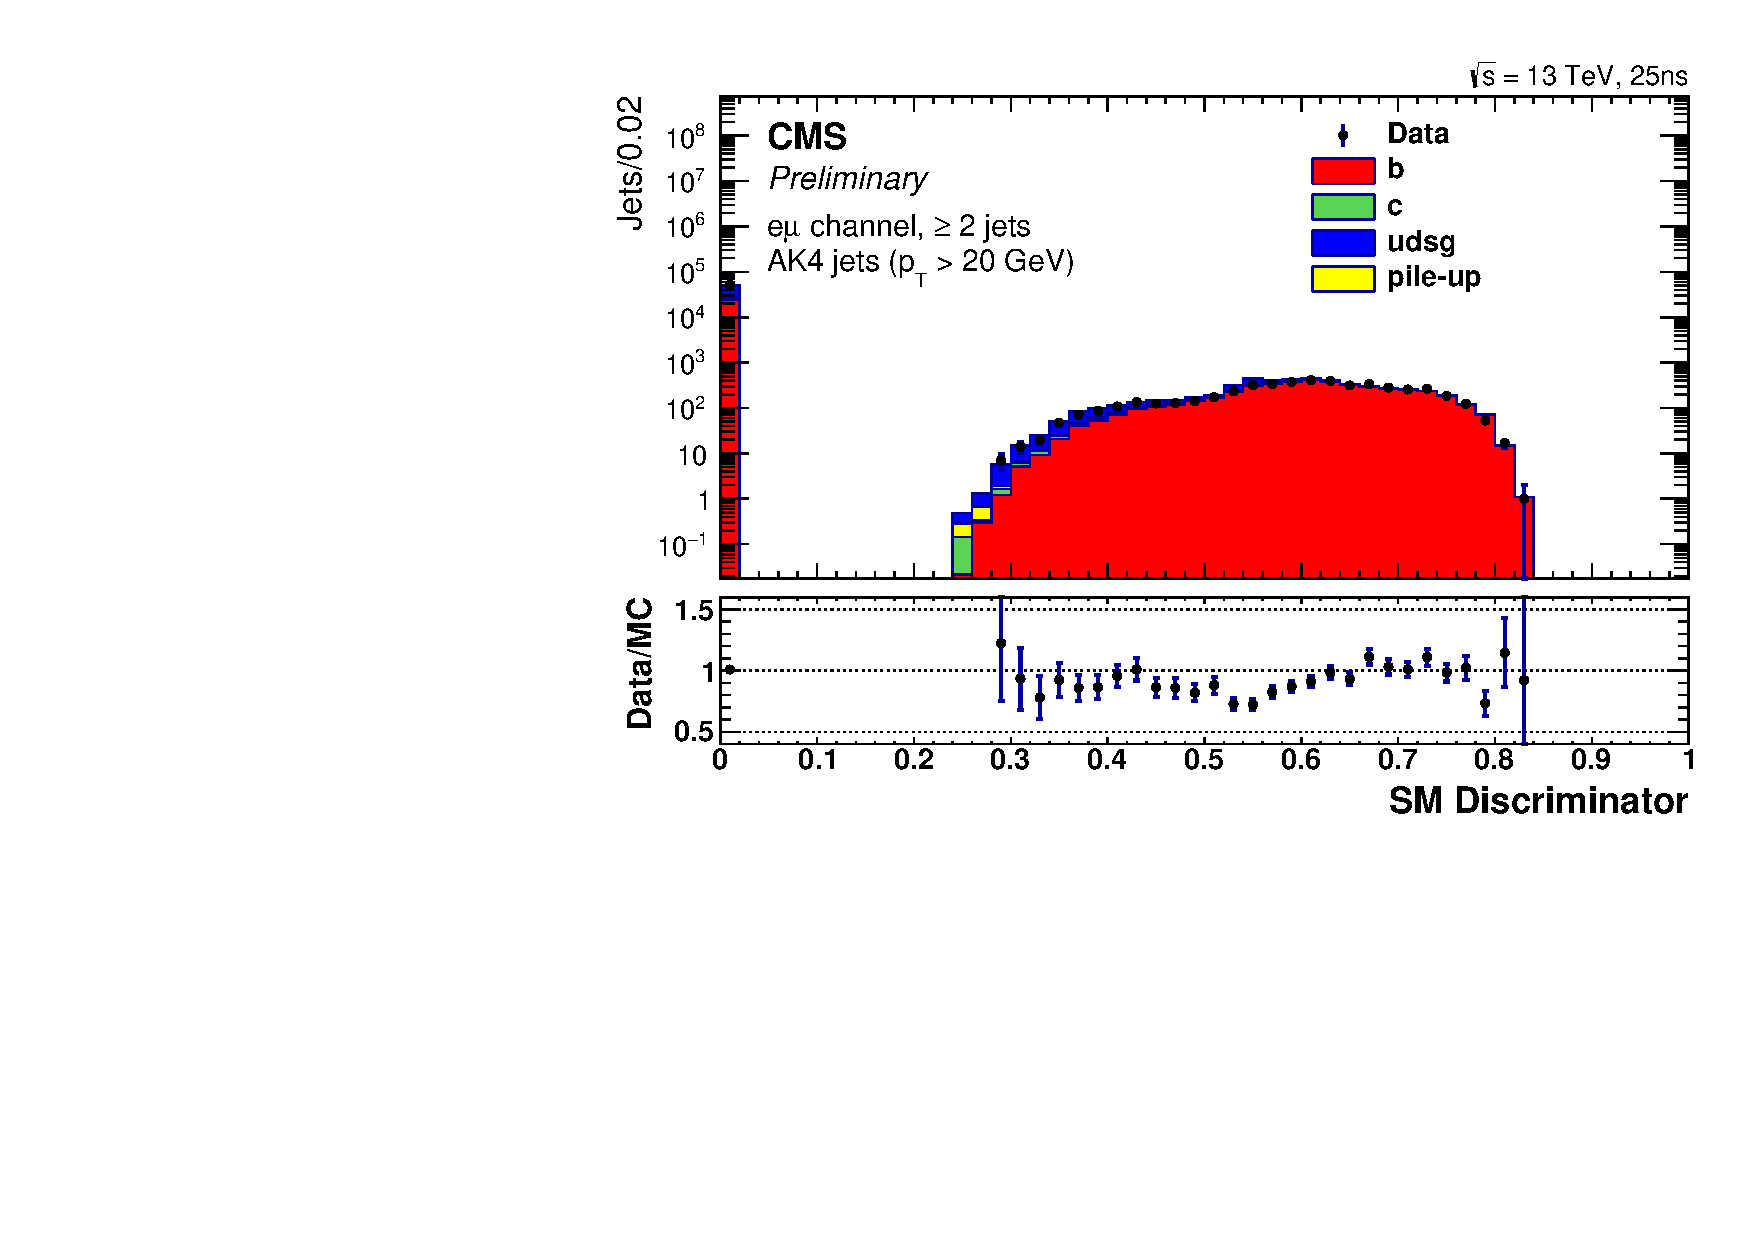
\includegraphics[width=0.5\textwidth]{figures/btv/softmu.pdf}} \\
\caption[The soft lepton b discriminator distributions]{The discriminator distributions of the soft lepton b taggers in dileptonic ($\mathrm{e\mu}$) \ttbar+jets events. The large fraction of jets with a soft muon discriminator value around 0 arises from cases where no muon was associated to the jet. Figures from~\cite{CMS-PAS-BTV-15-001}.}
\label{fig:btag_softlep}
\end{centering}
\end{figure}

\subsubsection{The CSVv2 b~tagger}
The Combined Secondary Vertex algorithm V2 (CSVv2) is based on the original CSV implementation introduced in Run I~\cite{Chatrchyan:2012jua} and uses machine learning to combine track and secondary vertex information such as vertex mass or flight distance. Based on the presence and quality of the secondary vertex, the CSVv2 is optimised in several categories:
\begin{itemize}
\item presence of a good secondary vertex, in which case the flight distance and other vertex related variables are defined
\item the pseudo-vertex category with two good tracks but no vertex fit, in which case the track parameters are used
\item a no vertex category that uses information only from displaced tracks.
\end{itemize}
The final CSVv2 discriminant is a likelihood combination of binary classifiers based on artificial neural networks with a single hidden layer in all 3 categories. The CSVv2 algorithm has been deployed on both the AVR vertices as CSVv2 (AVR) and the IVF vertices, denoted CSVv2 (IVF). The CSVv2 (IVF) has an efficiency of about~$66\%$~for b jets at a mistag rate for light jets (udsg-associated) of about~$1\%$~based on~\ttbar~simulation at the CSVv2 medium working point~\cite{CMS-PAS-BTV-15-001}. The CSVv2 b~discriminator is the primary b~tagging algorithm used in the end of Run I and the beginning of Run II at CMS. The discriminator distributions are shown on~\cref{fig:btag_csv}.

\begin{figure}
\begin{centering}
\subfloat[The CSVv2 AVR b~tagger]{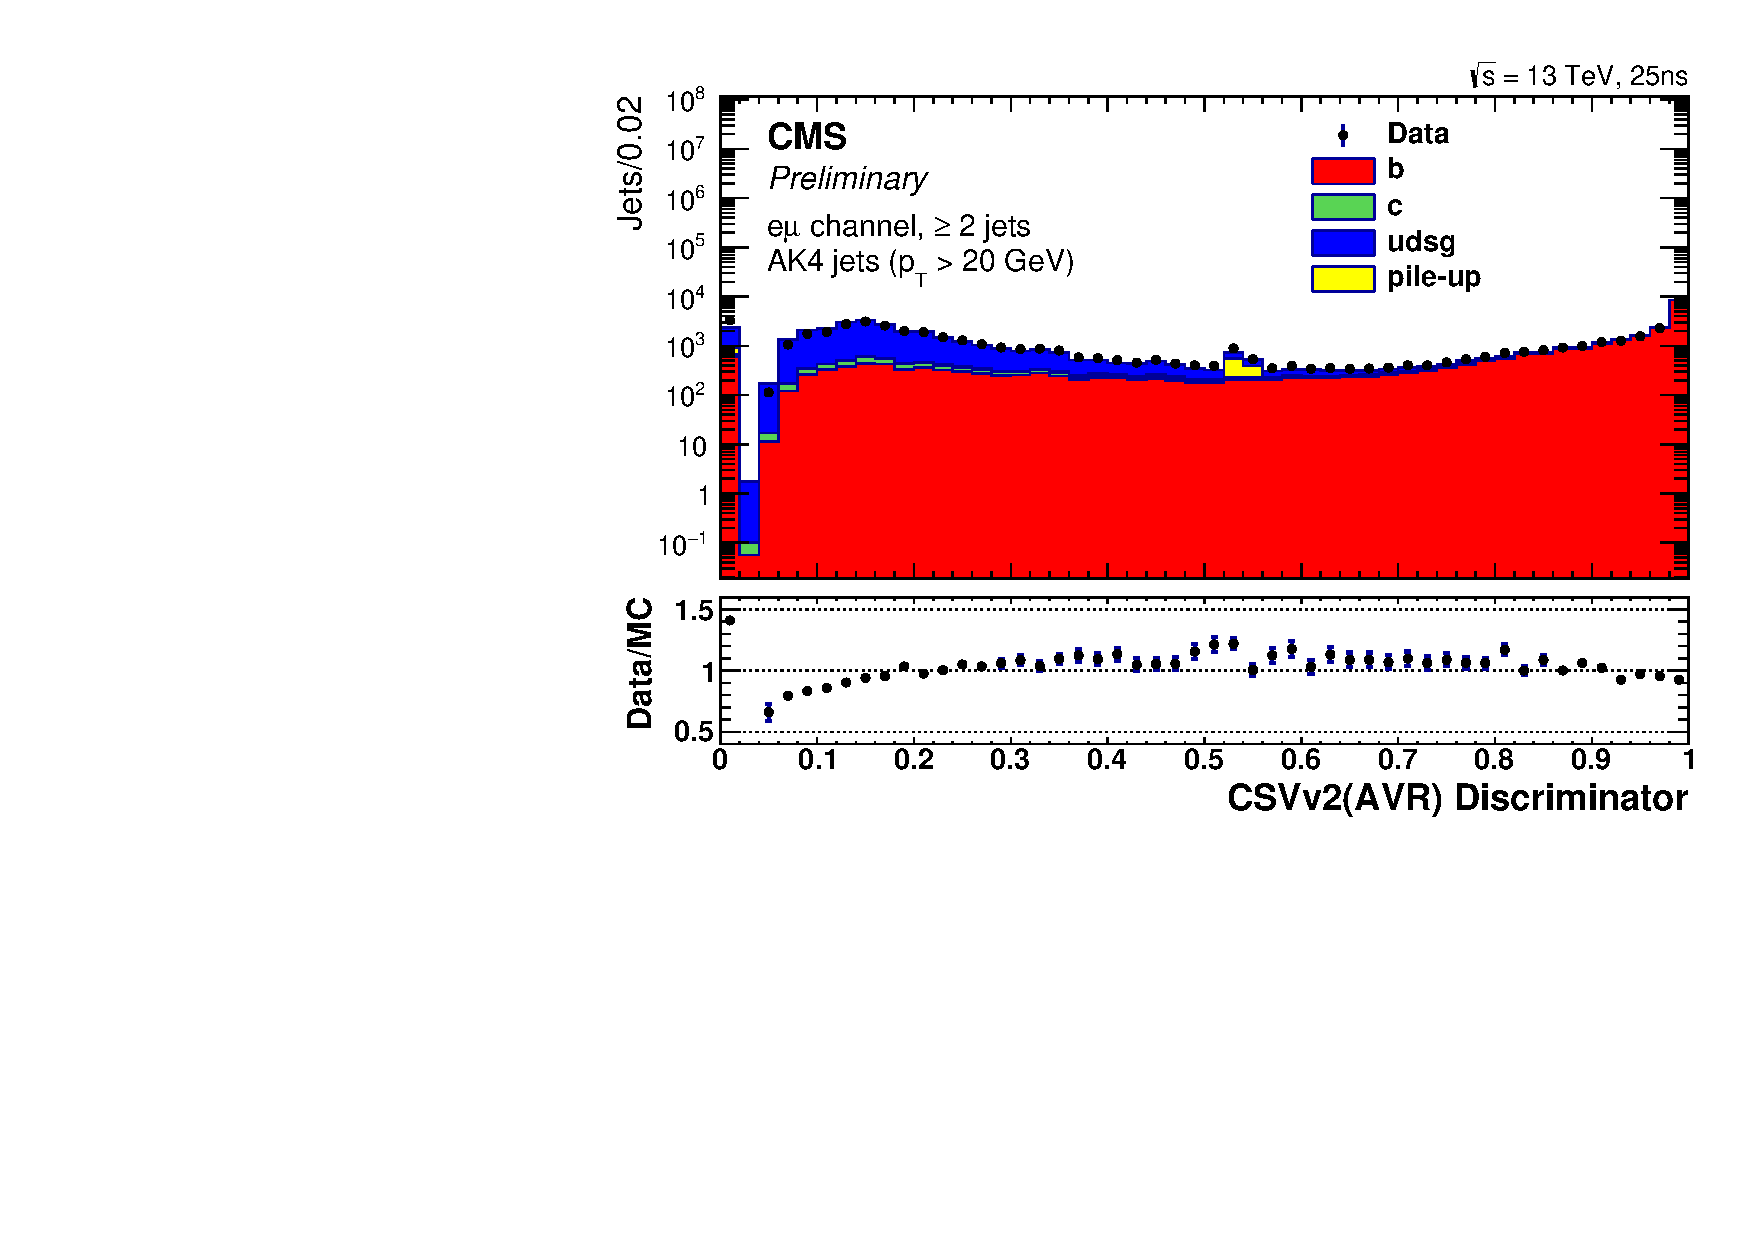
\includegraphics[width=0.5\textwidth]{figures/btv/csvavr.pdf}}
\subfloat[The CSVv2 IVF b~tagger]{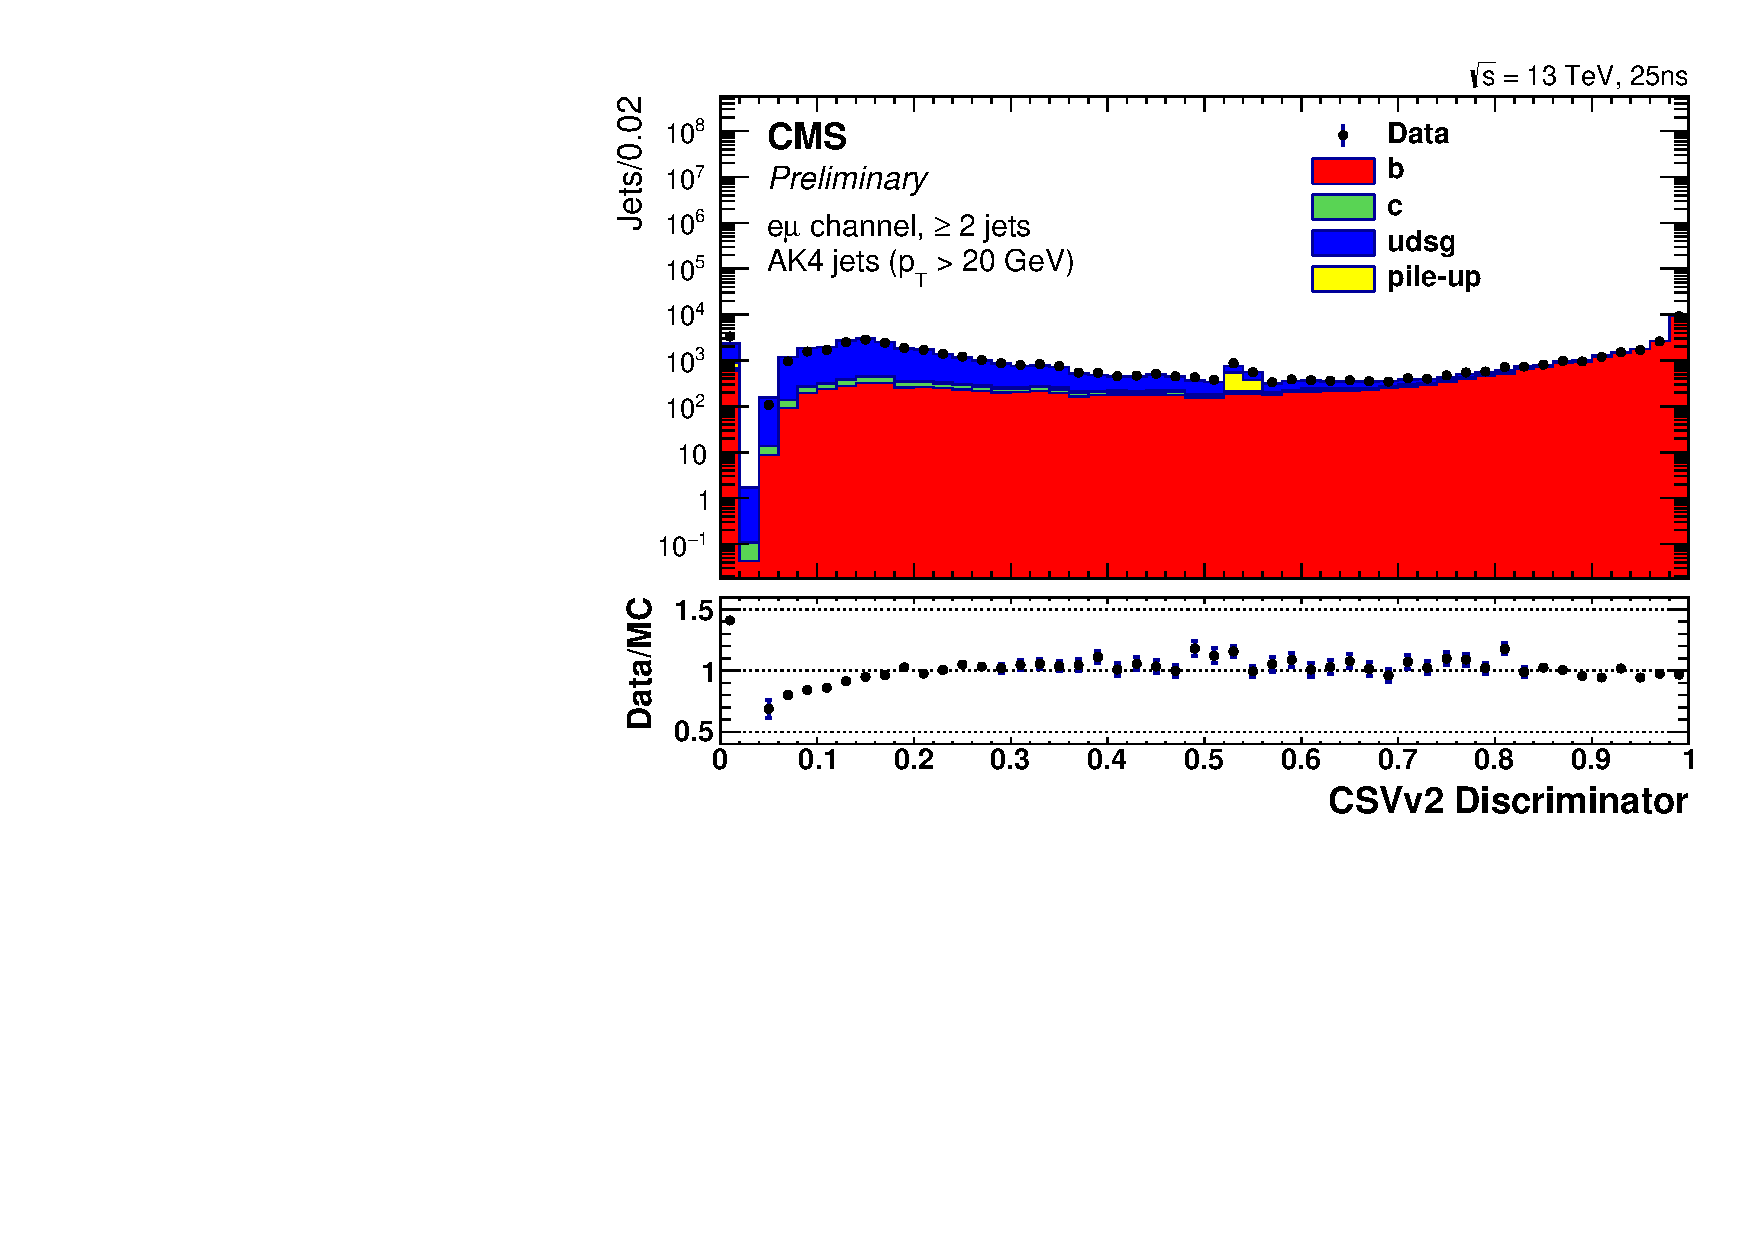
\includegraphics[width=0.5\textwidth]{figures/btv/csvivf.pdf}} \\
\caption[The CSVv2 b~tagger discriminator distributions]{The discriminator distributions of the CSVv2 b~taggers in dileptonic ($\mathrm{e\mu}$) \ttbar+jets events. Figures from~\cite{CMS-PAS-BTV-15-001}.}
\label{fig:btag_csv}
\end{centering}
\end{figure}

\section{The combined multivariate b~tagger}
In Run II, we have developed an improved b~tagger algorithm for CMS that combines the aforementioned individual b~taggers, relying on various sources of information, to a single discriminator using boosted decision trees (BDTs) via the \texttt{scikit-learn} package~\cite{scikit-learn}. This combined discriminator, denoted cMVAv2, exploits the fact that the AVR and IVF vertex reconstruction algorithms may reconstruct different vertices, the presence or lack of soft leptons and secondary vertex information simultaneously. The tagger is optimised on~\ttbar+jets simulation, with cross-validation on a multi-jet simulation sample. At a similar b-jet efficiency to the CSVv2 medium working point ($\epsilon_b \simeq 70\%$), the cMVAv2 b-tagger algorithm reduces the mistag rate for light jets from~$1\%$~to about~$0.5\%$, as seen on~\cref{fig:btag_roc}.

\begin{figure}
\begin{centering}
\subfloat[The b~tagging and misclassification probability.]{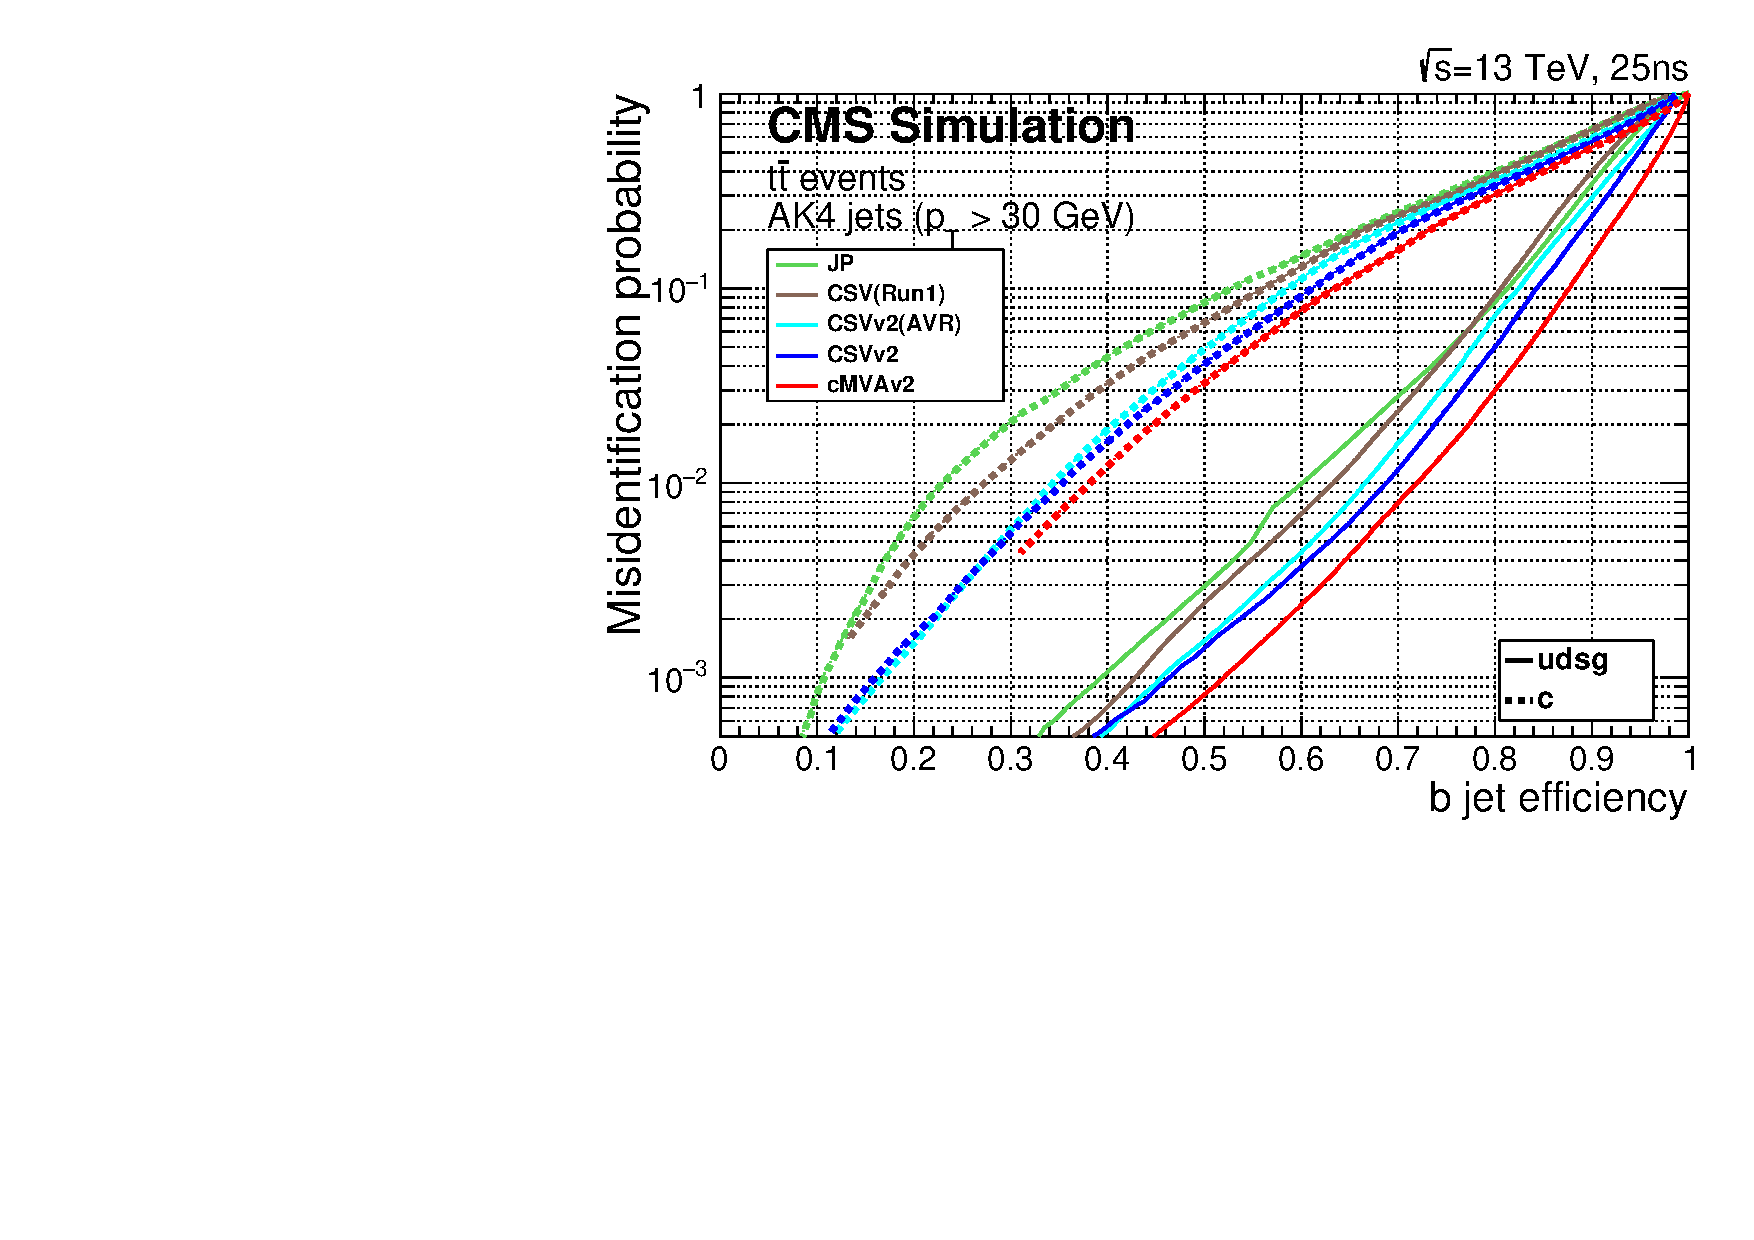
\includegraphics[width=0.5\textwidth]{figures/btv/Figure_008.pdf}}
\subfloat[The discriminant distribution for the cMVAv2 discriminator.]{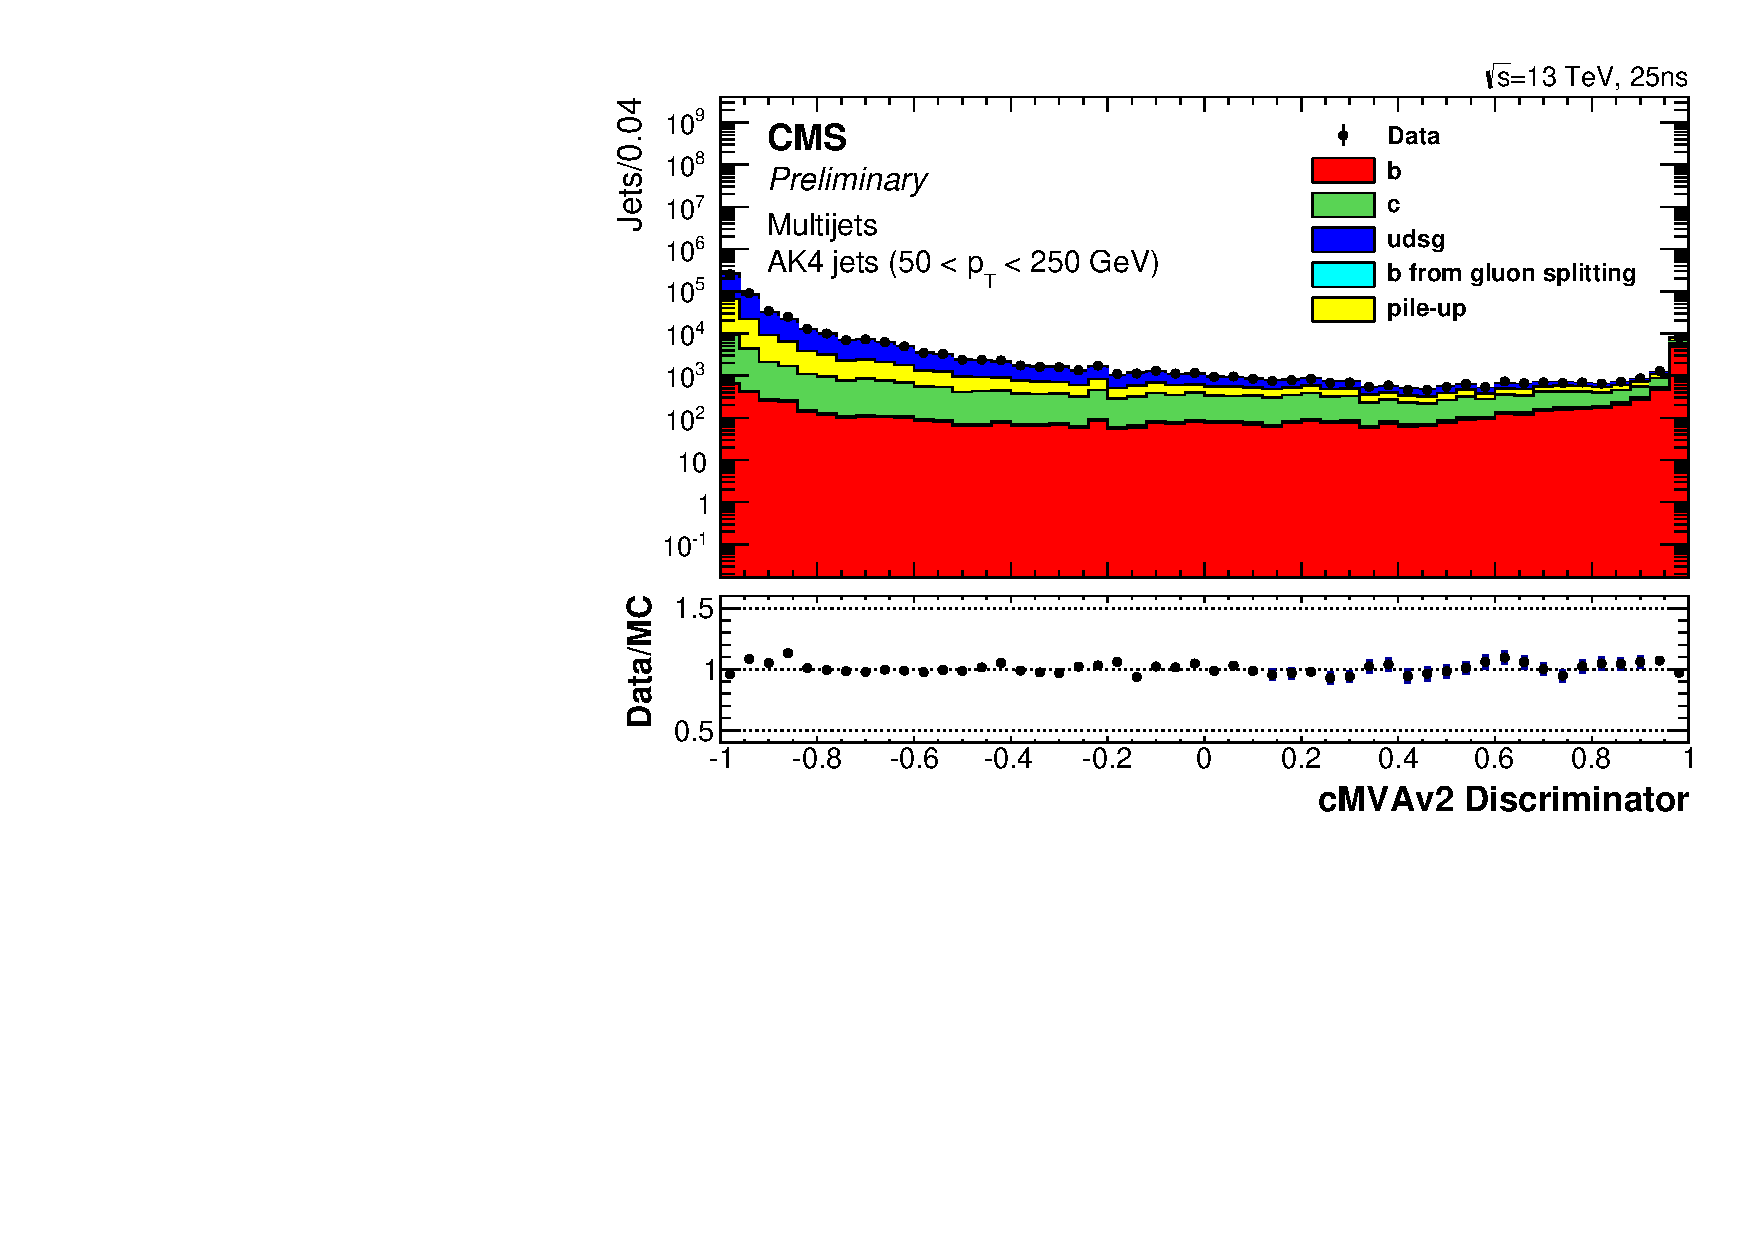
\includegraphics[width=0.5\textwidth]{figures/btv/Figure_007-a.pdf}} \\
\caption[The performance of the CMS b~taggers in Run II]{The performance of the CMS b~taggers in Run II. On~(\textbf{a}), the efficiency to correctly tag b~jets is shown with respect to the misclassification probability for light jets (udsg-associated, solid line) and charm jets (dashed line), based on~\ttbar+jets simulation. The medium working point correspond to a light jet efficiency of $\epsilon_{l} = 1\%$ and we see that the cMVAv2 b discriminator has~$\epsilon_{b} \simeq 72\%$, compared to the CSVv2 b-efficiency~$\epsilon_{b} \simeq 66\%$. On~(\textbf{b}), we show the comparison of the cMVAv2 discriminator between data and simulation, where data-driven scale factors are applied. Figures from~\cite{CMS-PAS-BTV-15-001}}
\label{fig:btag_roc}
\end{centering}
\end{figure}

\subsection{Implementation}
The cMVAv2 b~discriminator is a optimised as a binary classifier in a supervised training mode on jets derived from~\ttbar+jets simulation. Simulated jets are assigned a flavour by re-clustering the jet with momentum-scaled generator-level hadrons in such a way that the momentum of the jet is not altered. Based on the clustered hadrons, a jet is assigned to be a b jet, a c jet or a light jet in decreasing priority. We use particle flow jets with~$p_T > 20$~GeV,~$|\eta| < 2.5$~and enhance the selected jet sample at high~$p_T$~and~$|\eta|$~by limiting the amount of jets in the binned 2D distribution of~$p_T \in [20, 620], |\eta| \in [0, 2.5]$~with 100 bins per dimension to~$N_{\mathrm{max}} = 10000$~per bin. This sub-sampling technique effectively gives higher weight to the tails of the momentum and pseudorapidity distribution and reduces the simulated data to an amount that fits in the RAM of a conventional PC. We use an inclusive~\ttbar+jets sample generated with~\powheg~and \pythia~and an independent multi-jet sample generated with~\pythia~for cross-validation. We list the details of the simulated samples in~\cref{tab:btag_samples}.

\begin{table}[h!]
\begin{center}
\begin{tabular}{c|cccc}
\hline
MC sample & events & b jets & c jets & light jets \\
\hline
\ttbar+jets & 28M & 9.5M & 3.7M & 11M \\
multi-jet (QCD) & 29M & 1.2M & 2.3M & 17M \\
\hline
\hline
\end{tabular}
\caption[The training and validation samples for cMVAv2]{The simulated samples used for optimising and validating the cMVAv2 b~tagger. The jets are filtered with a~$p_T, |\eta|$-dependent selection that restricts the amount of jets in the high-statistics, low~$p_T$~and~$|\eta|$~part of the distribution.}
\label{tab:btag_samples}
\end{center}
\end{table}

\subsubsection{Kinematic reweighting}
Since the kinematic distributions in~$p_T$~and~$|\eta|$~of b, c and light jets are different due to their different production modes, we need to ensure that the b~tagger algorithm distinguishes between jets of different flavour based on quantities that are mostly independent of kinematics. In addition to the subsampling technique mentioned above, we reweight the jet sample used in the training of the binary classifier such that the distributions are roughly uniform in~$p_T$~and~$\eta$~using a weight~$w(p_T,|\eta|,\mathrm{flavor})$~derived on simulation, as shown on~\cref{fig:btag_pt_reweight}. This reweighting does not have a significant effect on the overall final b~tagging performance of the discriminator, however, it helps to make the optimisation less sample-dependent.

\begin{figure}
\begin{centering}
\subfloat[The jet~$p_T$~distributions by flavor.]{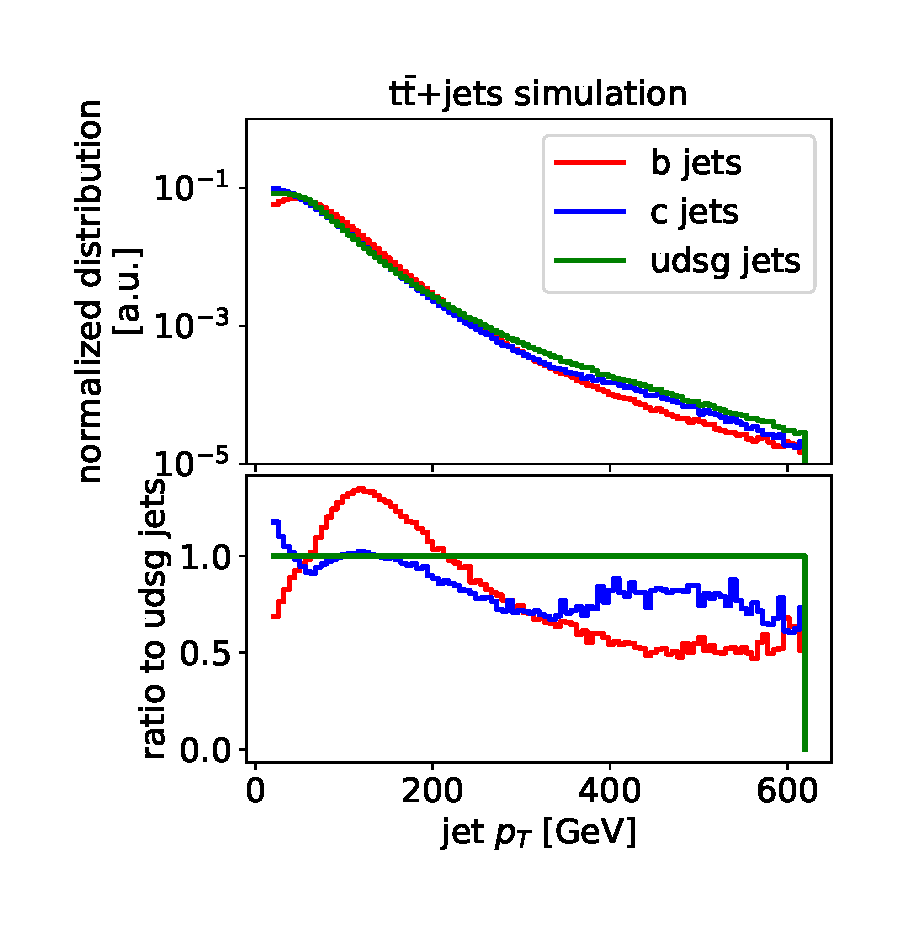
\includegraphics[width=0.5\textwidth]{figures/btv/jet_pt_flavor.pdf}}
\subfloat[The reweighted jet~$p_T$~distribution.]{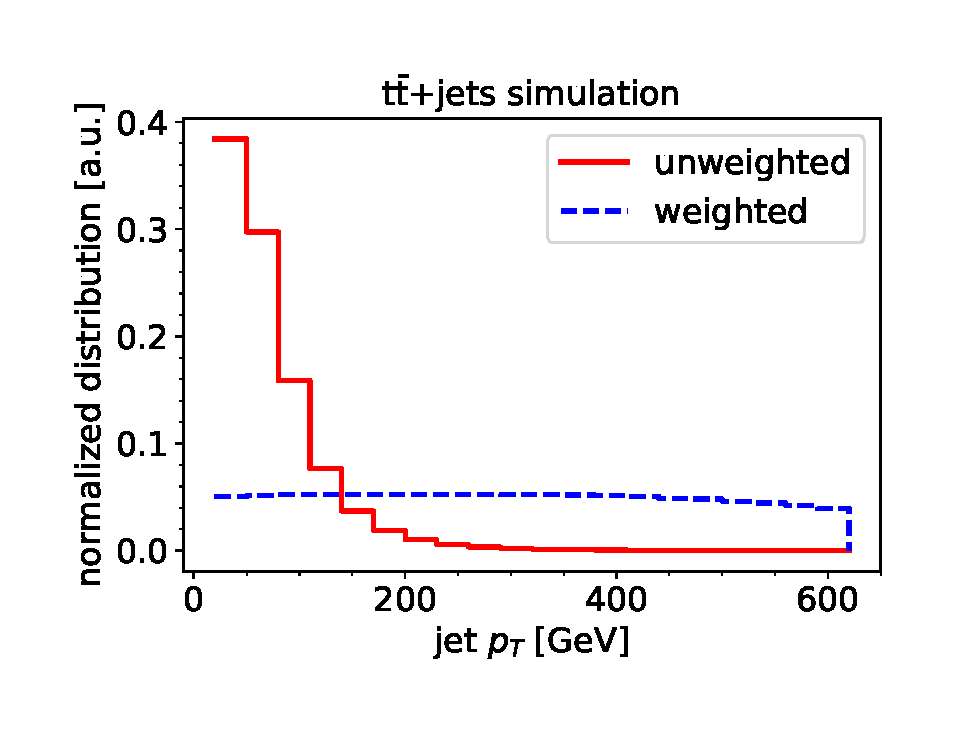
\includegraphics[width=0.5\textwidth]{figures/btv/jet_pt_weighted.pdf}} \\
\caption[Comparison of jet kinematics in MC simulation by jet flavour]{Comparison of jet kinematics by associated MC flavour before and after the kinematic reweighting. On~(\textbf{a}), we compare the jet~$p_T$~distributions for b, c and light jets. We see that b jets have a momentum distribution that is narrower and peaks around~100~GeV. On~(\textbf{b}), we show the jet~$p_T$~distribution before and after applying the kinematic reweighting~$w(p_T,|\eta|,\mathrm{flavor})$. We see that the reweighted distribution is roughly uniform, with small differences caused by simulation statistics in the derivation of the weight. These distributions are derived using~\ttbar+jets simulation.}
\label{fig:btag_pt_reweight}
\end{centering}
\end{figure}

\subsubsection{Input variables}
We have used the b~tagger algorithms described earlier as inputs to the cMVAv2 algorithm. In particular, we use the following 6 b~discriminators: CSV~(AVR), CSV~(IVF), JP, JBP, SoftMuon and SoftElectron. We have studied the correlation between CSV~(AVR) and CSV~(IVF), as shown on~\cref{fig:btag_csv_correlation}. Although the linear correlation coefficient is around~$C \simeq 0.9$~for all flavours, we see a non-negligible contribution from jets which have different vertices from the two vertexing algorithms and thus different CSV discriminator values. Therefore, we expect that a combined discriminator will outperform either of the two. Furthermore, the information provided by the JP and JBP discriminators can complement the CSV in cases no vertices could be found. To verify whether adding the additional input b~discriminators provides useful information for b~tagging, we optimise a set of BDT classifiers iteratively by including the 6 input discriminators one by one.

\begin{figure}
\begin{centering}
\subfloat[bottom jets]{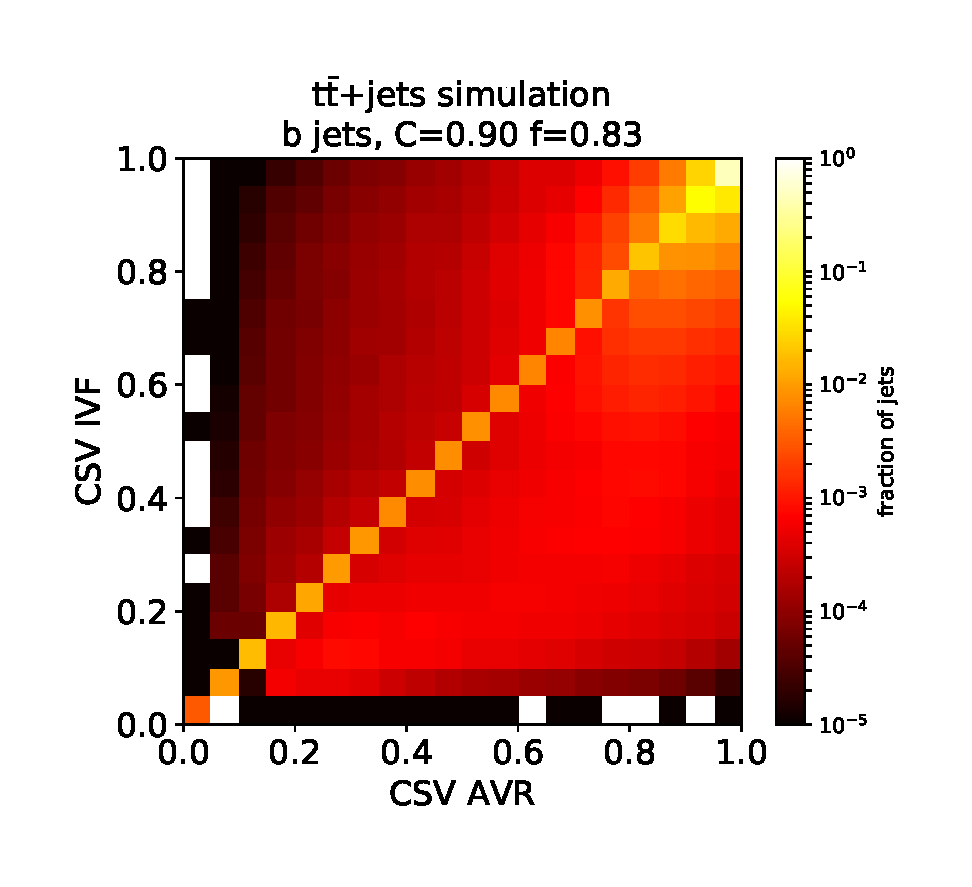
\includegraphics[width=0.35\textwidth]{figures/btv/CSV_AVR_IVF_corr_b.pdf}}
\subfloat[charm jets]{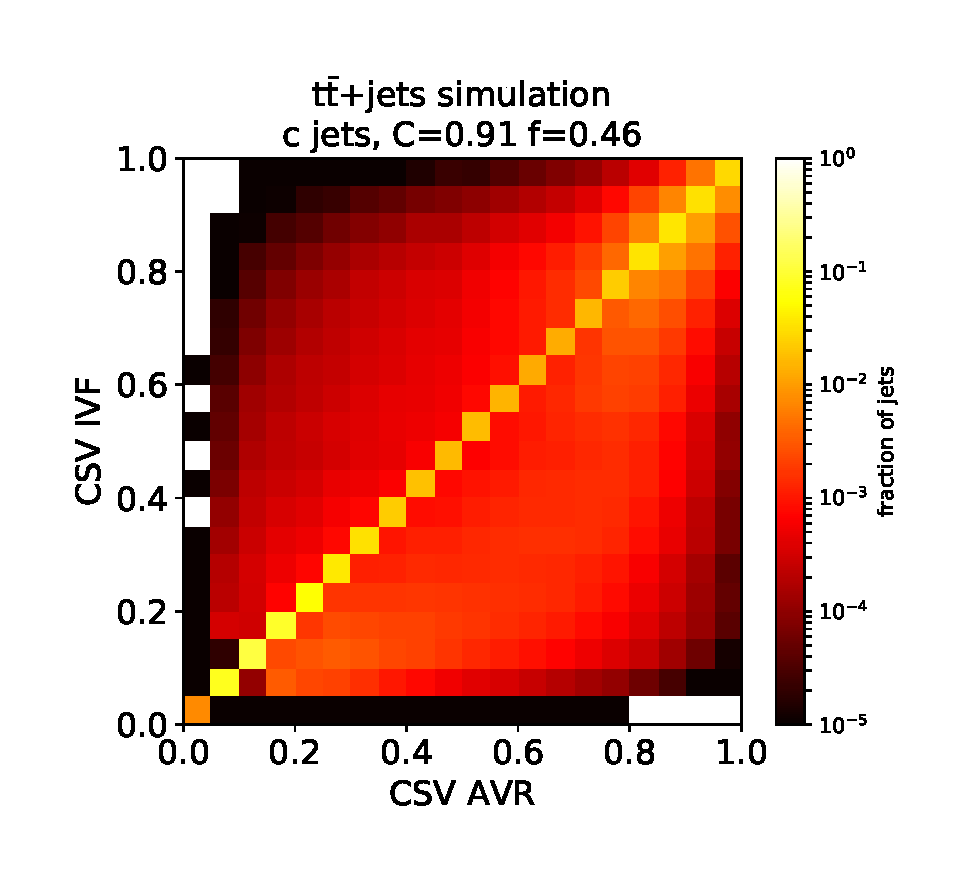
\includegraphics[width=0.35\textwidth]{figures/btv/CSV_AVR_IVF_corr_c.pdf}}
\subfloat[light~(udsg) jets]{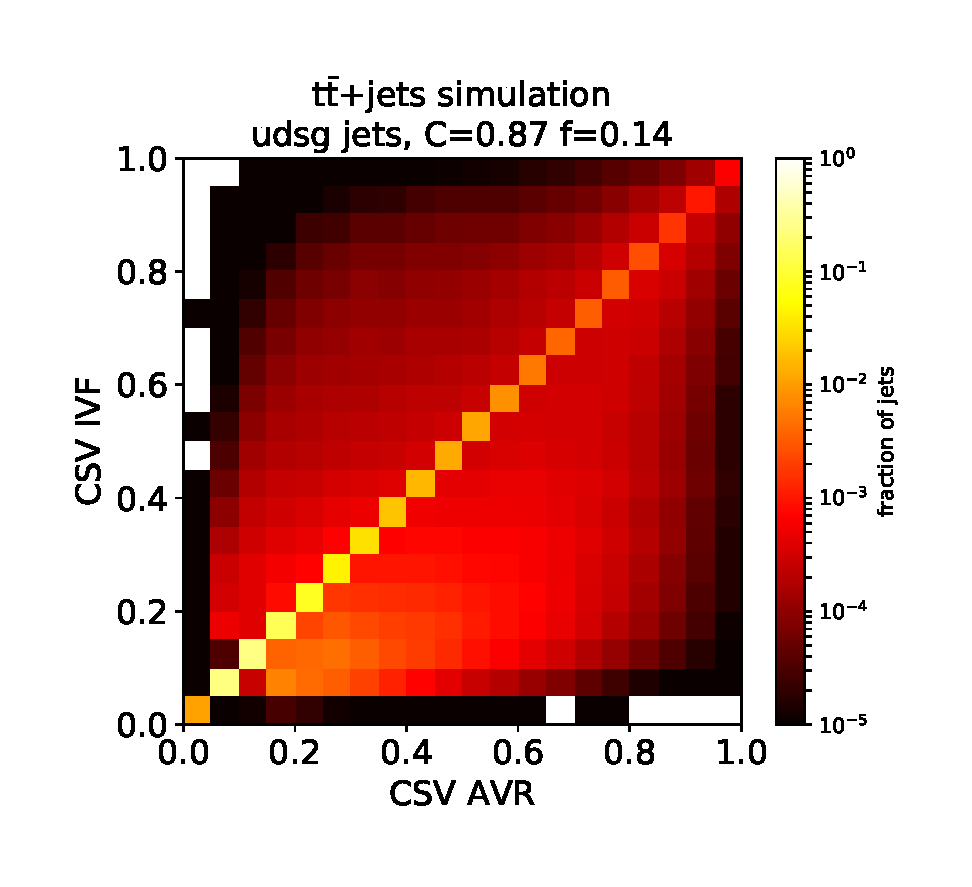
\includegraphics[width=0.35\textwidth]{figures/btv/CSV_AVR_IVF_corr_l.pdf}} \\
\caption[The correlation between the CSV b~discriminator value using AVR and IVF vertices]{The correlation between the CSV b~discriminator value using AVR and IVF vertices. Despite the high linear correlation coefficient~$C$, we see a significant fraction of jets~$f$~with non-equal values of the two discriminators, visible as the non-diagonal elements in the 2D distribution. These distributions are derived using the~\ttbar+jets~simulation.}
\label{fig:btag_csv_correlation}
\end{centering}
\end{figure}

\subsection{optimisation and validation}
In order to convince ourselves of the BDT optimisation, we perform a number of validation steps. The optimisation and validation of the BDTs is done on statistically independent subsets of the~\ttbar~+jets simulation sample and the statistical over-training is negligible after 200 boosting iterations, as can be seen on~\cref{fig:btag_loss}. This is due to the large amount ($\mathcal{O}(10^7)$ jets) of available simulation statistics, combined with the input variable space being relatively low-dimensional~($N=6$). We have further validated the training using $k$-fold cross-validation, where the training is repeated $k$ times on sub-samples of the data, and found the statistical uncertainty between sub-samples to be negligible.

\begin{figure}
\begin{centering}
\subfloat[The loss function (top) with respect to boosting iteration and the difference between training and validation loss (bottom).]{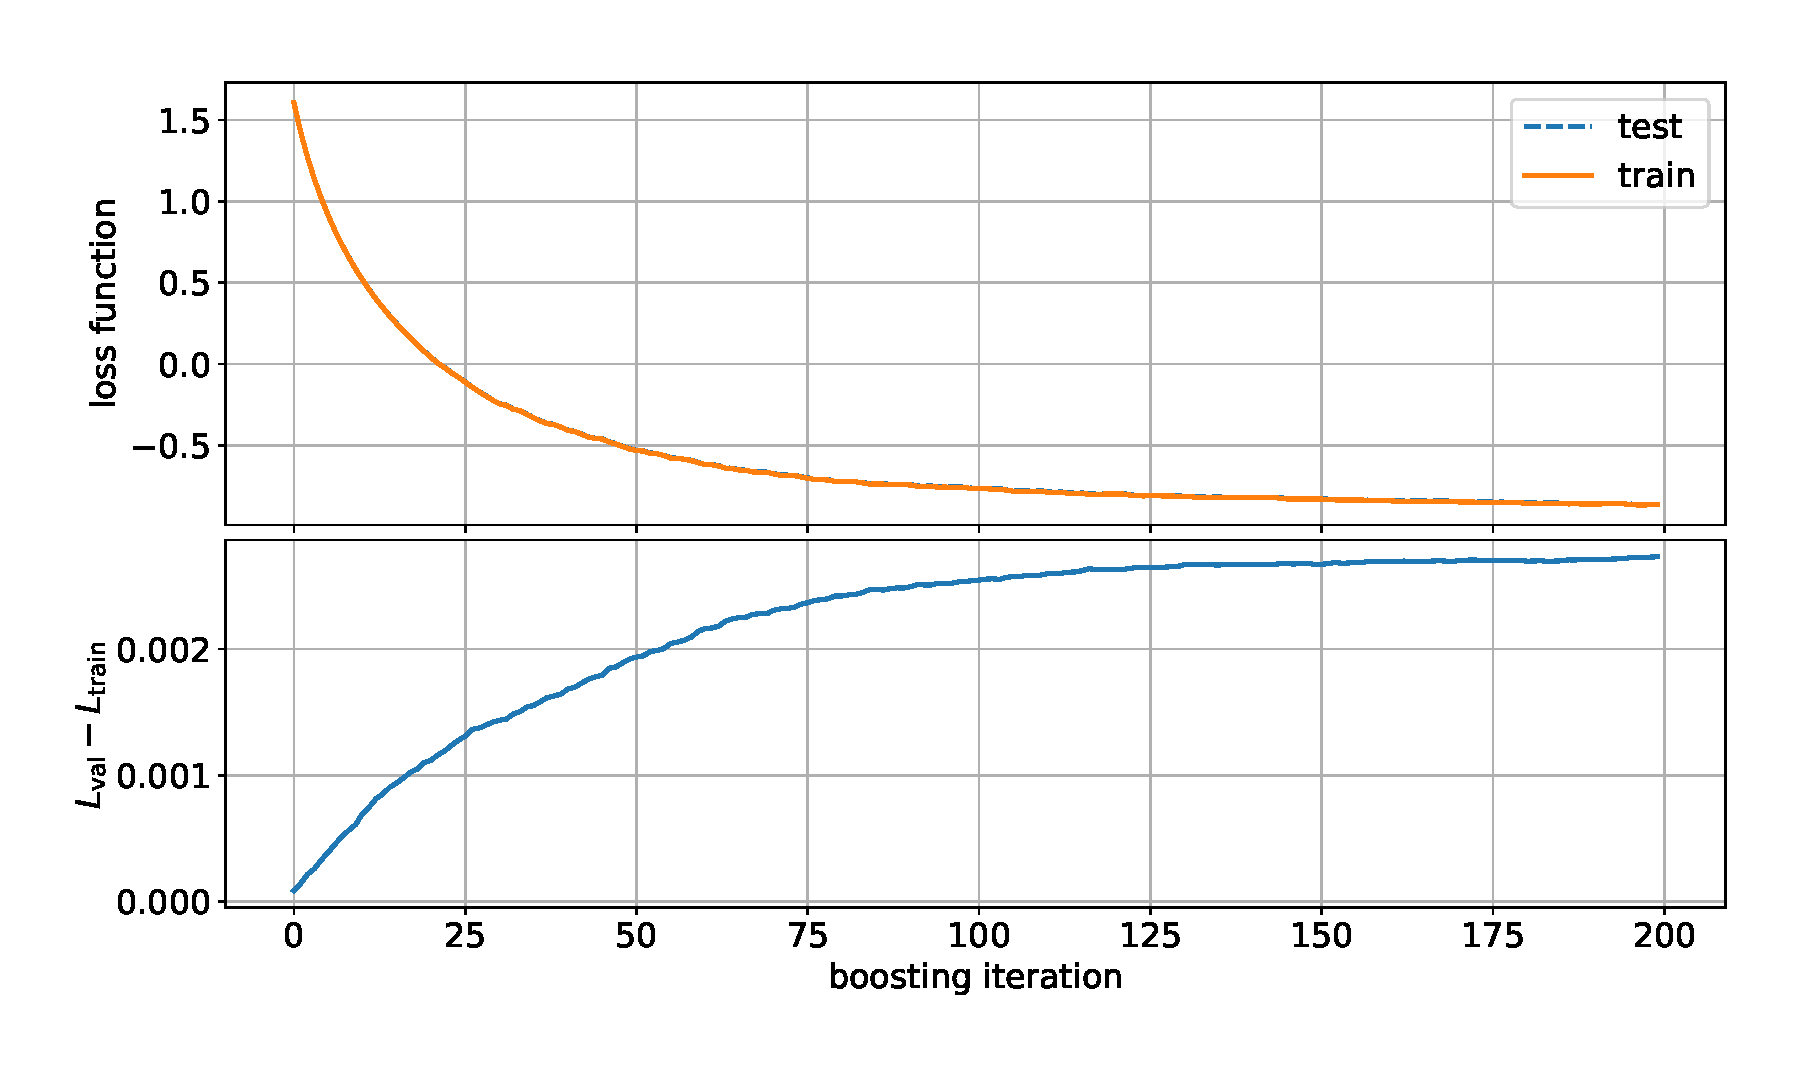
\includegraphics[width=0.7\textwidth]{figures/btv/loss.pdf}} \\
\subfloat[Ratio of discriminator distributions.]{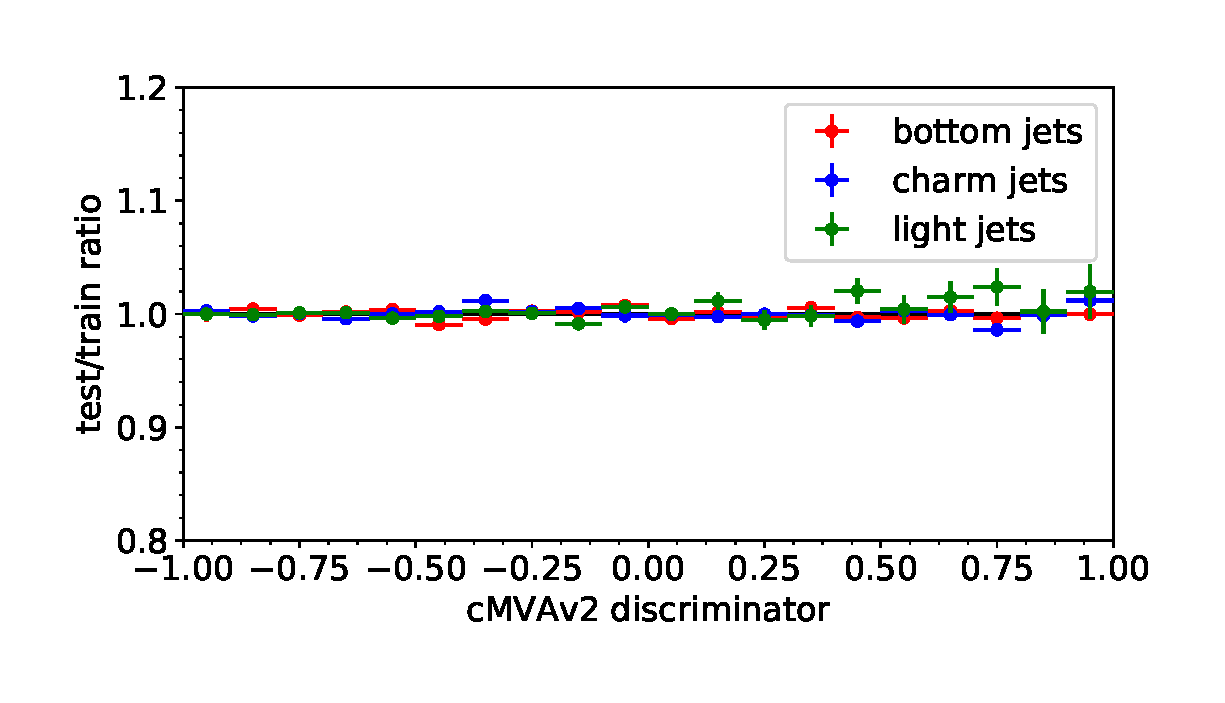
\includegraphics[width=0.7\textwidth]{figures/btv/train_test_distribution.pdf}}
\caption[The cMVAv2 BDT loss as a function of boosting iteration]{Validation of the cMVAv2 against over-training by comparing the loss function between the training set and the statistically independent validation set as a function of the boosting iteration on~(\textbf{a}). We see good convergence after~$N=200$~boosting steps, with a negligible difference between the loss functions. Furthermore, on~(\textbf{b})~we compare the discriminator distributions on the training and test sets, with the ratio being compatible with unity within statistical uncertainties.}
\label{fig:btag_loss}
\end{centering}
\end{figure}

We analyse the performance of the optimised b~discriminator in terms of the efficiency for selecting b jets~(signal) with respect to charm and light jets~(background). On~\cref{fig:btag_cmva_roc}, we show the ROC AUC performance metric of the various stages of cMVAv2 optimisation. In general, we see that the BDTs are able to take advantage of all the input taggers, with the inclusion of each input improving the overall discrimination power monotonically. The optimisation is carried out on the~\ttbar~+jets simulation sample and we have cross-checked the results against the multi-jet simulation, where we have seen an equivalent improvement.

\begin{figure}
\begin{centering}
\subfloat[b vs light jets]{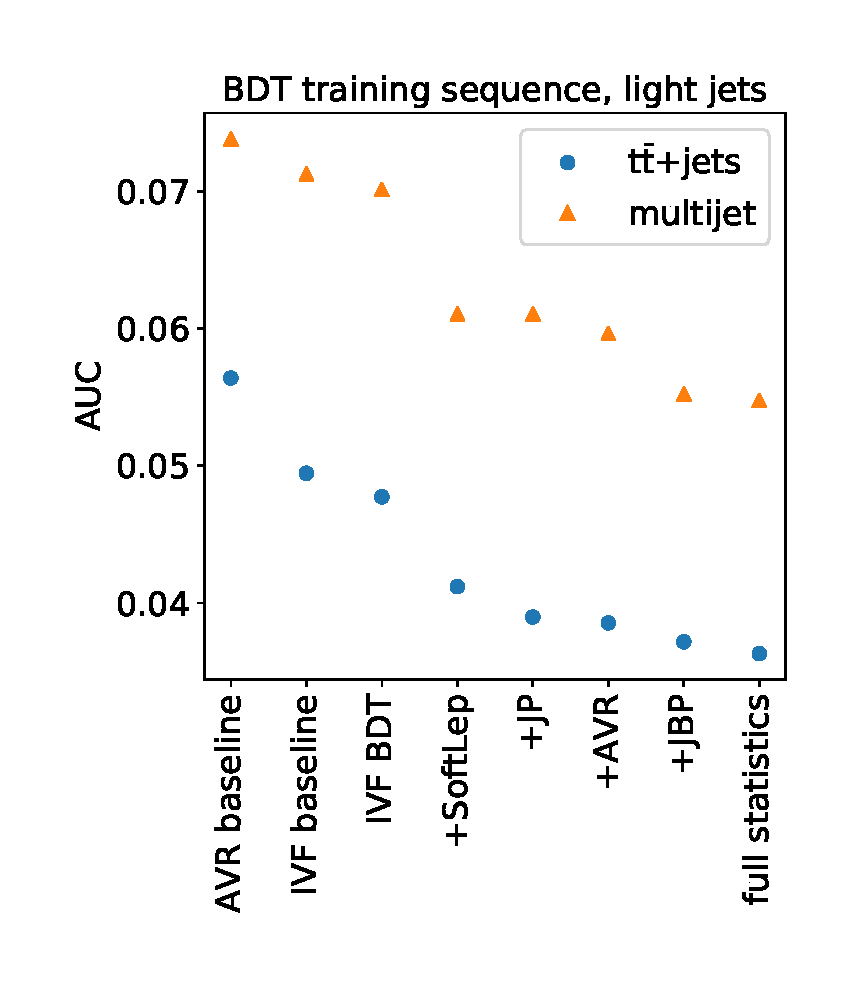
\includegraphics[width=0.5\textwidth]{figures/btv/bdt_seq_light.pdf}}
\subfloat[b vs charm jets]{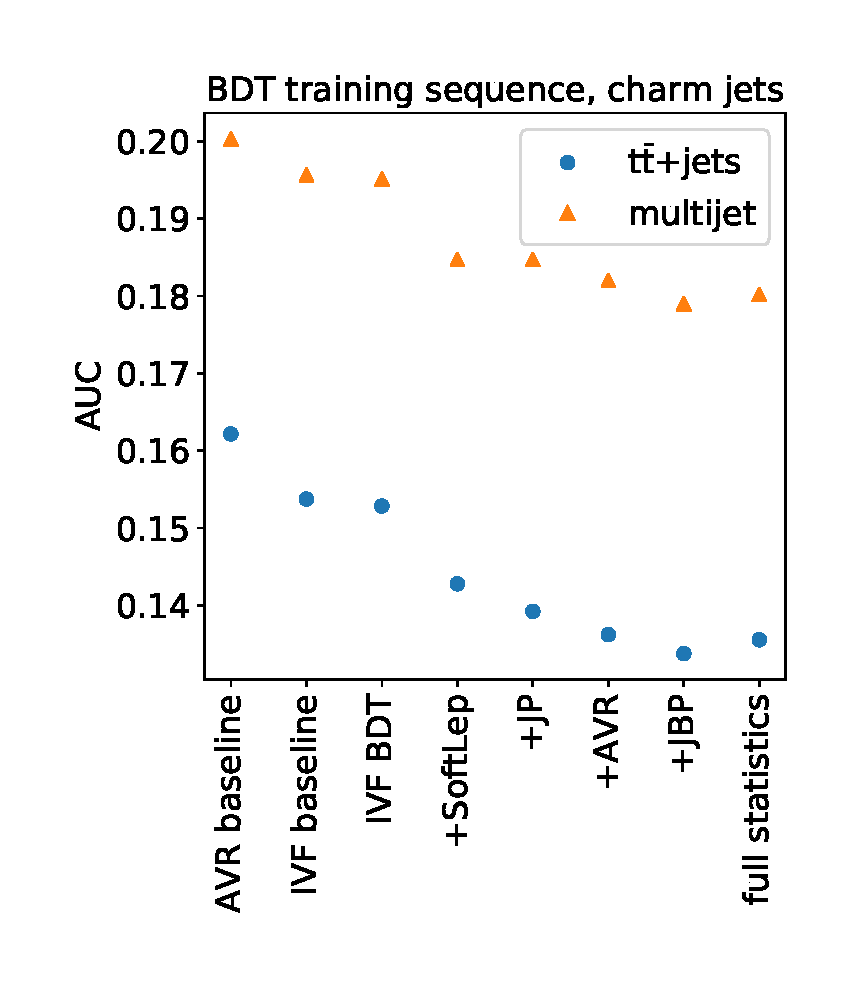
\includegraphics[width=0.5\textwidth]{figures/btv/bdt_seq_charm.pdf}} \\
\caption[The cMVAv2 performance as a function of training variables.]{The performance characteristic ROC AUC as a function of the number of variables included in the BDT training, where lower values correspond to better discrimination. The baseline CSV b~discriminators with IVF and AVR vertices are compared to the cMVAv2, which is optimised by successively including the IVF, SoftLepton, JP, AVR, JBP taggers with partial training statistics. We see that the inclusion of the Soft Muon and Soft Electron b~taggers provides a significant improvement to the b jet vs. light jet discrimination (\textbf{a}), as well as b jet vs. charm jet (\textbf{b}). The best discrimination against light jets is reached by using the full simulation sample. We have performed the optimisation on the~\ttbar~+jets simulation sample, and cross-checked the results on the multi-jet sample. Statistical uncertainties on the performance are verified using cross-validation and are negligible.}
\label{fig:btag_cmva_roc}
\end{centering}
\end{figure}

The performance of the optimised cMVAv2 b~discriminator is validated by comparing the efficiency of selecting light jets or charm jets as b~tagged at a fixed b~tagging efficiency for b~jets as a function of jet kinematics, as shown on~\cref{fig:btag_kinematics}. We see that the cMVAv2~b~discriminator has somewhat more stable performance with respect to jet kinematics than the CSV b~discriminators and an improved discrimination power in the forward region $|\eta| > 1.5$. The cMVAv2~b~discriminator uniformly outperforms the CSV algorithm over the studied jet momentum range $20 < p_T < 320$,~$0 < |\eta| < 2.5$. Overall, the cMVAv2 algorithm has a mistagging efficiency lower by at least~$20\%$~($10\%$) for light jets (charm jets) over the full range.

\begin{figure}
\begin{centering}
\subfloat[light jet efficiency in $p_T$]{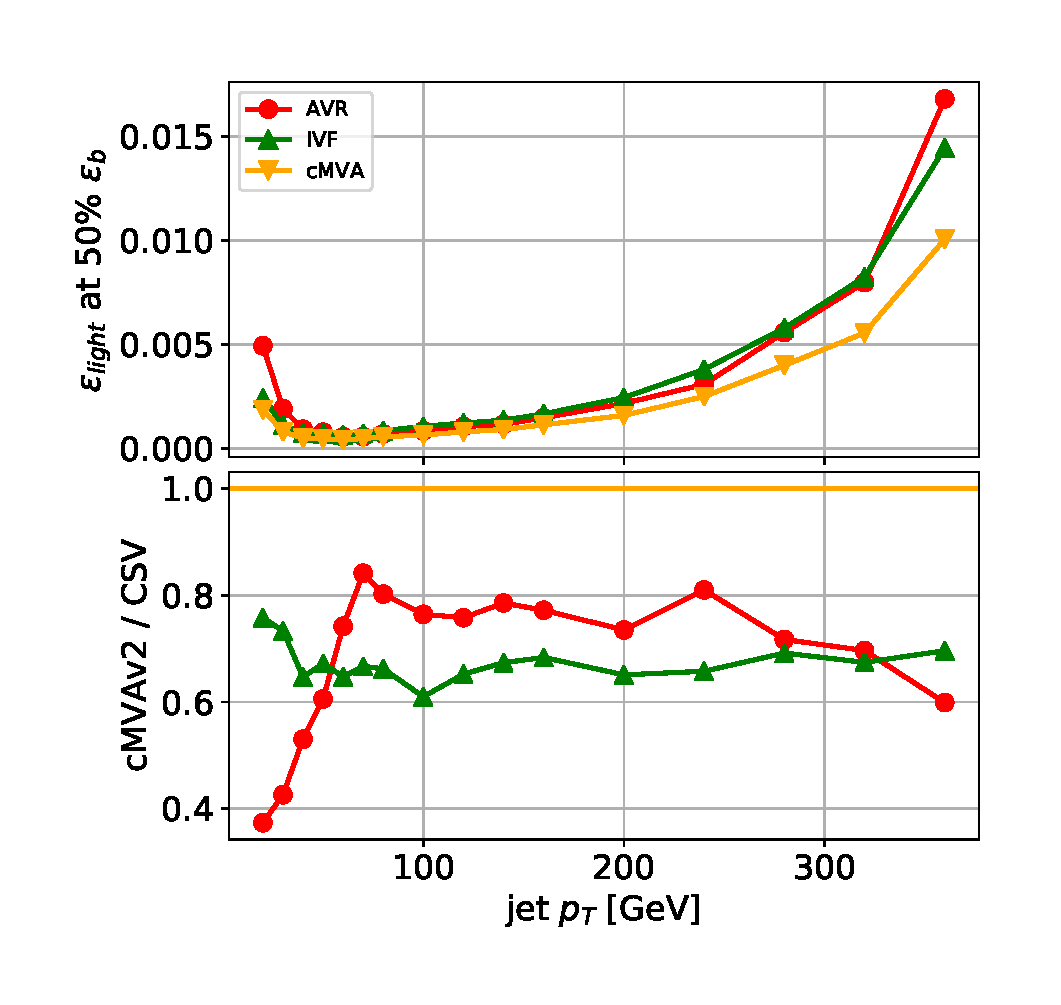
\includegraphics[width=0.5\textwidth]{figures/btv/tt_e50_l_pt.pdf}}
\subfloat[light jet efficiency in $|\eta|$]{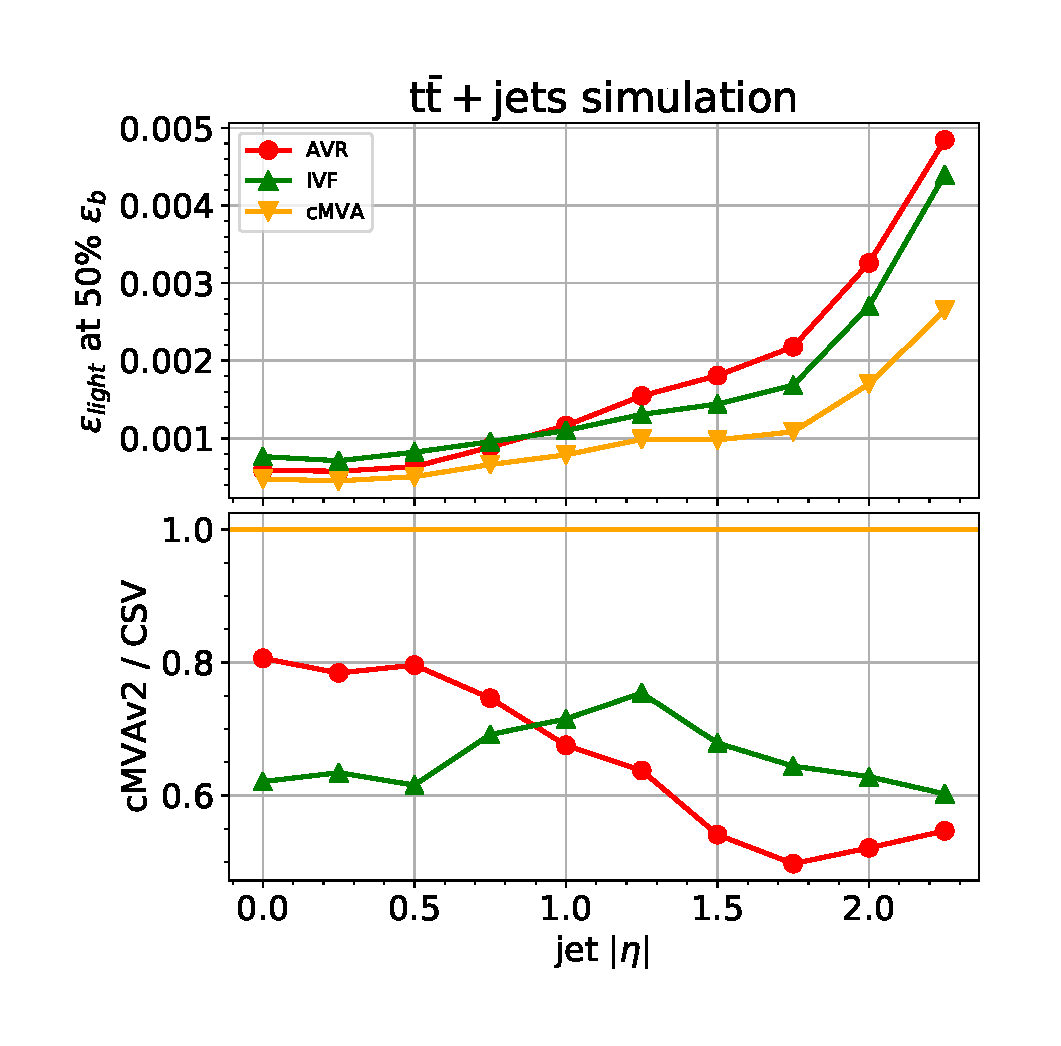
\includegraphics[width=0.5\textwidth]{figures/btv/tt_e50_l_eta.pdf}} \\
\subfloat[charm jet efficiency in $p_T$]{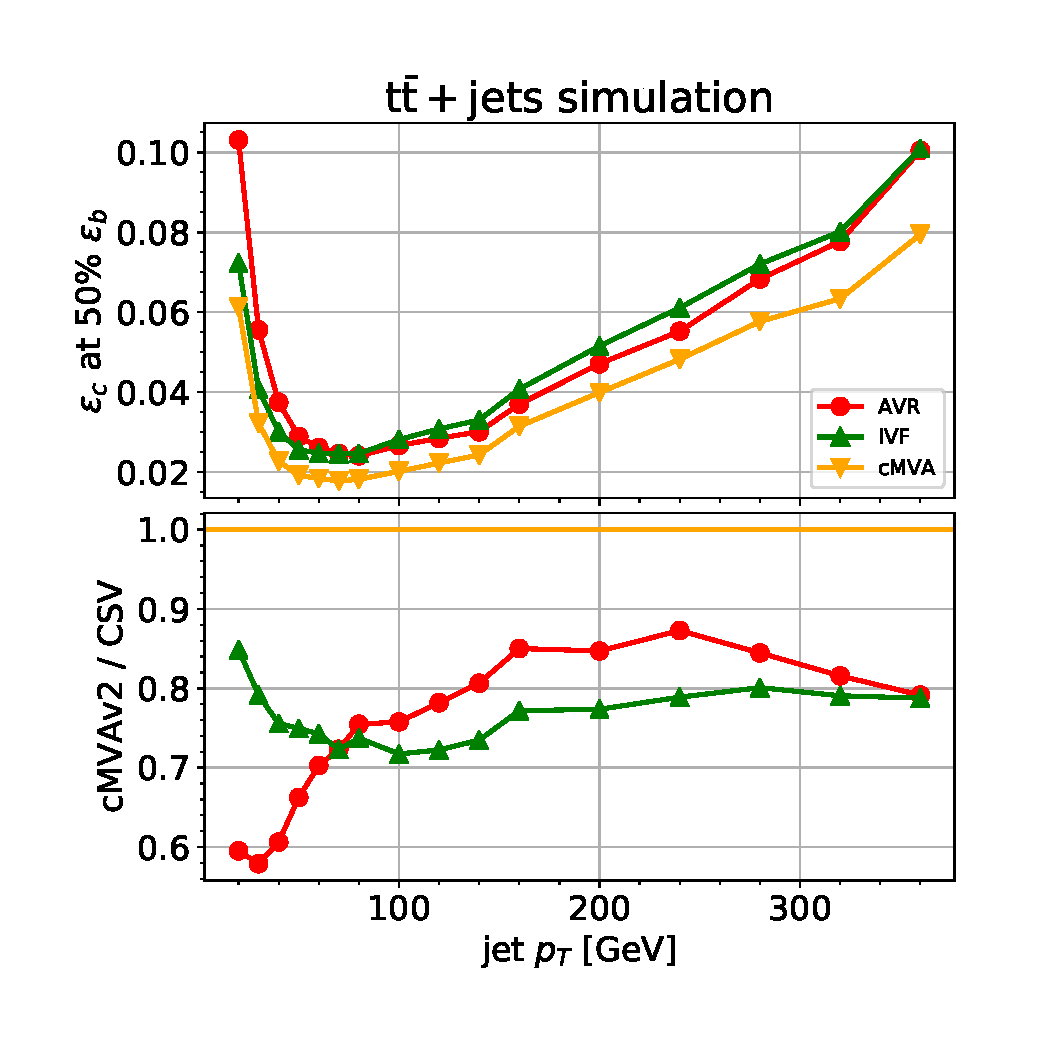
\includegraphics[width=0.5\textwidth]{figures/btv/tt_e50_c_pt.pdf}}
\subfloat[charm jet efficiency in $|\eta|$]{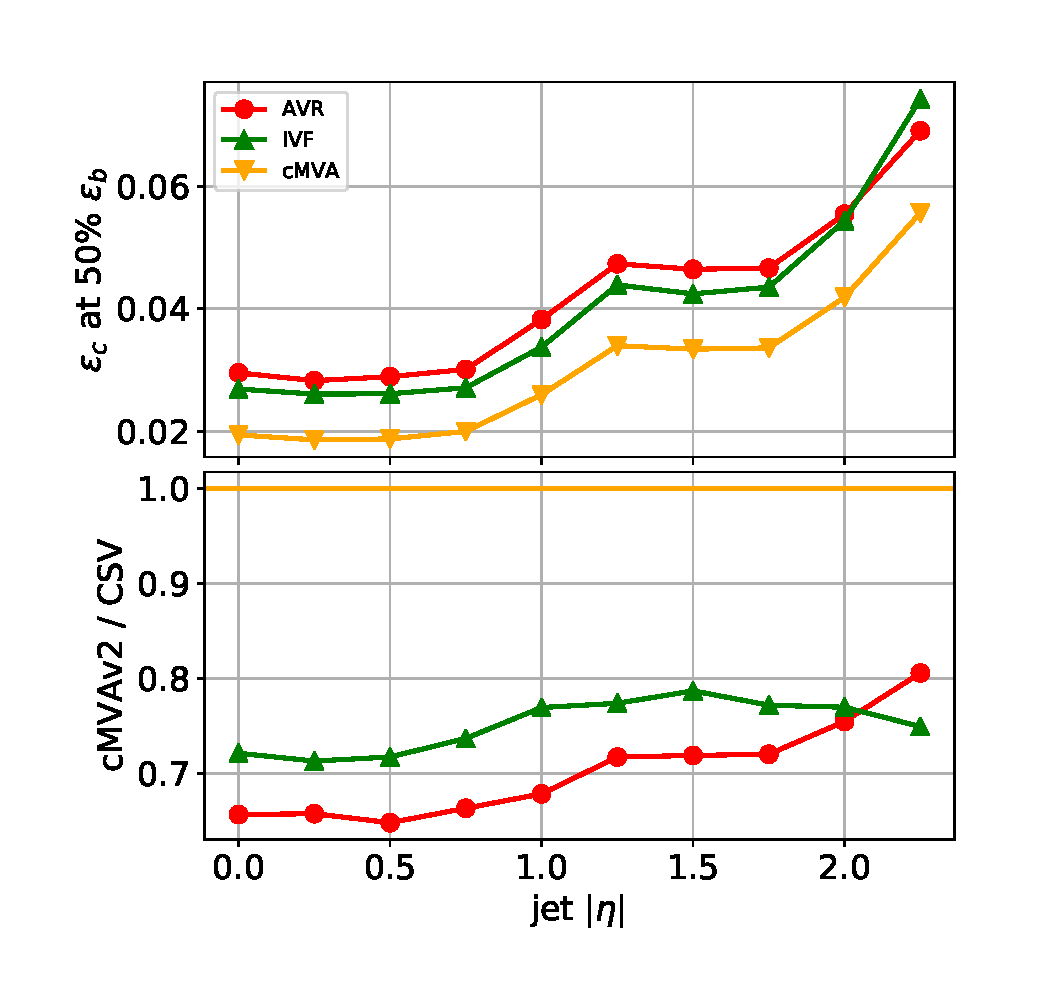
\includegraphics[width=0.5\textwidth]{figures/btv/tt_e50_c_eta.pdf}} \\
\caption[The cMVAv2 mistagging probability as a function of jet kinematics.]{The $p_T$ and $|\eta|$-dependent mistagging efficiency at a fixed $\epsilon_{b}$ in~\ttbar~+jets simulation. We compare the cMVAv2 discriminator to the CSV IVF and AVR discriminators in terms of the light jet and charm jet efficiency (mistagging) at the working point with~$50\%$~b~jet efficiency. We see that the cMVAv2 discriminator performs well over a wide~$p_T$~and~$|\eta|$~range, with $\epsilon_{\mathrm{light}}$ in the forward region being around~$40\%$ lower than for the CSV algorithm. While the efficiency of the algorithm overall still depends on jet kinematics due to the inherent correlation between the kinematics and the underlying variables sensitive to b-tagging, the dependence is somewhat lower for cMVAv2 than for CSV.}
\label{fig:btag_kinematics}
\end{centering}
\end{figure}

The final validation and calibration of the cMVAv2 algorithm was done using the tag counting method, where the b~tagging efficiency and the corresponding scale factor between data and simulation is determined from \ttbar+jets dilepton events relying on the $\mathrm{t} \rightarrow \mathrm{b} \mathrm{W}^+$ decay and thus the presence of 2 true b~jets. The correction for the light jet mistagging efficiency is extracted from multi-jet events based on the discriminator distribution using jets with only negative impact parameters and thus enriched in light jets. The cMVAv2 discriminator corrections have independently been determined with the differential reweighting method described further in~\cref{sec:object_id_btag} and the results are compatible with scale factor derived from tag counting~\cite{CMS-PAS-BTV-15-001}. 

The evaluation of the cMVAv2 b~tagger has been implemented in \texttt{CMSSW} independently of the optimisation. As such, the cMVAv2 was one of the two default b discriminators of CMS during the 2016 data-taking period. In order to interface the decision trees optimised using \texttt{scikit-learn} to the CMS online software in \texttt{CMSSW}, we have developed a stand-alone library~\cite{mlglue} to convert between BDT implementations form several commonly used open source machine learning toolkits, namely \texttt{scikit-learn}, \texttt{xgboost} and \texttt{TMVA}. The set of decision trees was then exported as a stand-alone payload to the~\texttt{CMSSW} environment, such that the cMVAv2 b~discriminator could be deployed through standard reconstruction software by simply evaluating the decision trees.

\section{Summary}
We have developed an improved b~tagging algorithm, the cMVAv2, for Run II which combines the discrimination power in several independently optimised b~discriminators using different vertexing algorithms and different subsystems of the detector. The cMVAv2 b~discriminator outperforms the present state of the art at CMS by  
The cMVAv2 algorithm was optimised using BDT algorithsm commonly used in the  
%\section{Matrix Element Method}
\label{sec:mem}

\subsection{Hypothesis testing}

\subsection{Optimal test statistic}
\label{sec:test_statistic}

\subsection{Description of MEM}

The MEM is a multivariate analysis technique in which we directly compute the per-event probability density that depends on model parameters $\vec{\theta}$

\begin{equation}
P_{\vec{\theta}}(\vec{y}) = \frac{1}{\sigma}
\frac{\mathrm{d}\sigma_{\vec{\theta}}(\vec{y})}{\mathrm{d}\vec{y}}
\end{equation}
and use it in hypothesis testing as component of the test statistic. Through the differential cross section, the MEM explicitly depends on $\vec{y} = (\tilde{p}_{i \in \mathrm{jets}}, \tilde{p}_{i \in \mathrm{leptons}}, \dots)$, the vector containing the detector-level 4-momenta of the reconstructed particles, in particular, jets and leptons. The differential cross-section(\cref{eq:diff_cross_section}) depends on the squared matrix element $|\mathcal{M}^2|$ that we use to directly take into account the dynamics of the relevant underlying processes. The kinematics of the $2 \rightarrow n$ scattering process are encoded in the $n$-body phase space element(\cref{eq:n_body_phase_space}), where the delta function enforces the conservation of momentum between the initial and final state particles.

\begin{equation}
\label{eq:diff_cross_section}
\mathrm{d}\sigma_{\vec{\theta}} = \frac{(2\pi)^4 |\mathcal{M}_{\vec{\theta}}|^2}{4 \sqrt{(q_1 \cdot q_2)^2 - m_1 m_2}} \times
\mathrm{d}\Phi_n(q_1 + q_2; p_1, \dots, p_{n})
\end{equation}

\begin{equation}
\label{eq:n_body_phase_space}
\mathrm{d}\Phi_n = \delta^4 (q_1 + q_2 - \sum_{i=1}^n p_i) \prod_{i=1}^n \frac{\mathrm{d}^3 p_i}{(2\pi)^3 2 E_i}
\end{equation}
We have to consider several additional effects:
\begin{itemize}
\item We cannot directly observe the momenta of the initial state particles $q_1$ and $q_2$ in a proton-proton collision.
\item We do not measure the momenta of the neutrinos or jets that do not pass a transverse momentum threshold and the detector has a finite energy resolution.
\item We do not know which of the observed jets are matched to which partons.
\item The non-zero final transverse momentum caused by large-angle initial state radiation, spoiling the momentum balance in \cref{eq:n_body_phase_space}.
\end{itemize}

To address the first issue, we need to use parton density functions $g(x_{1,2})$ to weight the differential cross-section, integrating over the momentum fractions $x_{1,2} = E_{q_{1,2}}/E_{\mathrm{beam}}$.

In order to take into account detector effects, we integrate over unmeasured or poorly measured quantities using a transfer function $W(\vec{y}, \vec{p})$.
The transfer function relates final state parton-level quantities $\vec{p}$ to measurable quantities on the detector level $\vec{y}$ and encodes our knowledge about detector resolution or reconstruction efficiencies.

The question of jet-to-parton matching is addressed by summing over the $N_a$ possible permutations of jet-to-parton matching, which depends on assumptions about the process and the number of observed final state particles and is encoded in the exact factorized form of the transfer function $W(\vec{y}, \vec{p})$.

Finally, the modelling of the non-zero transverse recoil $\vec{\rho}_T = -\sum_{i=1}^n \vec{p}_{i,T}$ is treated empirically using a transfer function $\mathcal{R}(\tilde{\vec{\rho}}_T, \vec{\rho}_T)$ determined on simulation that relates the parton-level transverse momentum of the system $\vec{\rho}_T$ to the observed recoil $\tilde{\vec{\rho}}_T$. 

The evaluation of $|\mathcal{M}_{\vec{\theta}}|^2$ requires full knowledge of the initial and final state momenta, as well as the parameters of the model, summarized in $\vec{\theta}$. In particular, the parameters of the model contain the hypothesis $\mathcal{H} \in \{\ttH, \ttbb\}$ about the underlying process and the assumptions about which of the partons formed reconstructed jets $\mathcal{C}$, such that $\vec{\theta} = (\dots, \mathcal{H}, \mathcal{C})$. In the case of \ttH with the top quark pair decaying semileptonically $\ttH \rightarrow (\ell^- \bar{\mathrm{\nu}}_\ell) \mathrm{b}\ (\mathrm{q} \mathrm{q}' \bar{\mathrm{b}})\ (\mathrm{b} \bar{\mathrm{b}})$, we may consider the fully reconstructed category where all 6 of the final state partons are reconstructed as jets, denoted as $2_W 2_H 2_t$, the case where one of the quarks from the hadronic decay $\mathrm{W} \rightarrow \mathrm{q} \mathrm{q}'$ is out of acceptance, denoted as $1_W 2_H 2_t$ and so forth, such that $\mathcal{C}_{\mathrm{SL}} \in \{ 2_W 2_H 2_t, 1_W 2_H 2_t, \dots \}$. The number of unknown quantities to be integrated over depends on the reconstruction category $\mathcal{C}$, as described in detail in the next section. 
Thus, the per-event probability density takes the form
\begin{align}
\label{eq:mem_definition}
P(\vec{y}, \vec{\theta}) &= \sum_{k=1}^{N_a} \int \frac{\mathrm{d}x_1 \mathrm{d}x_2}{2 x_1 x_2 s} \int \prod_{i=1}^{n} \frac{\mathrm{d}^3 p_i}{(2\pi)^3 2 E_i} \\
&\times \delta^4 (q_1 + q_2 - \sum_{i=1}^n p_i)\\
&\times g(x_1) g(x_2) \\ 
&\times \mathcal{R}(\tilde{\vec{\rho}}_T, \vec{\rho}_T) \\ 
&\times |\mathcal{M}_{\vec{\theta}}(q_1, q_2, p_1, \dots, p_n)|^2 \\
&\times W(\vec{y}, \vec{p})
\end{align}

After having been first proposed for reconstructing events with missing momentum\cite{Kondo1988}, the MEM has been used in Tevatron for Higgs boson searches\fix and a precise measurement of the top quark mass\cite{D0topmass2004}. After first phenomenological studies showed that MEM could be used effectively for \ttH in a multi-parton final state\cite{Artoisenet2013}, it has been used in searches for \ttH by the CMS and ATLAS experiments in Run I of the LHC\fix. The MEM approach is closely related to MELA\cite{Gao} that has been extensively used in $\mathrm{H} \rightarrow \mathrm{ZZ} \rightarrow 4\mathrm{l}$ searches and $J^P$ measurements, however, in MELA, unreconstructed particles and transfer functions are not considered and the matrix elements have generally simple analytical forms.
In the following, we discuss in detail the implementation and improvements that were made to the MEM for Run II.

\subsection{Implementation}
\label{sec:mem_implementation}
In the case of semileptonic or dileptonic \ttH final state, the observables $\vec{y}$ consist of the energies (or equivalently transverse momenta) and the directions of the jets, the momenta of the charged leptons and the measured recoil of the system $\tilde{\vec{\rho}}_T$. As \cref{eq:mem_definition} needs to be integrated numerically, we first need to define it explicitly in terms of variables that are convenient and suitable for integration, namely energies, solid angles and combinations of invariant masses. The Jacobian transformation can be done analytically for both the top and antitop quarks and is of the form shown in \cref{eq:phase_space_jacobian}.
\fix
\begin{align}
\label{eq:phase_space_jacobian}
\fix
\end{align}

The scattering amplitude written as $|\mathcal{M}(\vec{p})|^2$ depends only on particle momenta, hence it is implied to be summed over spin and colour states. Furthermore, we treat the production and decay of the top quarks, W and Higgs bosons in the narrow-width approximation\cite{Berdine2007}, meaning we factorize the production and decay of these particles, as seen in \cref{eq:scattering_nwa}.

\begin{align}
\label{eq:scattering_nwa}
|\mathcal{M}_{\ttH \rightarrow (qq'b) (qq'\bar{b}) (b\bar{b})}|^2 &= |\mathcal{M}_{gg \rightarrow \ttH}(g_1, g_2, t, \bar{t}, h)|^2 \\
&\times \prod_{r = t,\bar{t}} \bigl[ \frac{\pi}{m_t \Gamma_t} \delta(t^2 - m_t^2) |\mathcal{M}_t(q,\bar{q},b)|^2 \bigr]_r \\
&\times \frac{\pi}{m_t \Gamma_t} \delta(h^2 - m_H^2) |\mathcal{M}_H(b,\bar{b})|^2
\end{align}

The decay amplitude of the top quark, assuming NWA for the W-boson, is given in \cref{eq:decay_top} and for the $\mathrm{H} \rightarrow \mathrm{b}\bar{\mathrm{b}}$ in \cref{eq:decay_higgs}.

\begin{equation}
\label{eq:decay_top}
FIXME
\end{equation}

\begin{equation}
\label{eq:decay_higgs}
FIXME
\end{equation}

\subsubsection{Transfer functions}
\label{sec:transfer_functions}

The transfer function $W(\vec{y} | \vec{p})$ maps a point $\vec{p} \in \Omega$ in the phase space to a point $\vec{y} \in \mathcal{A}$ in the space of reconstructed variables and it is ensured to be normalized to unity using \cref{eq:transfer_normalization}, which means that in an observable fiducial region, a phase space point has an efficiency $\epsilon(\vec{p}) \leq 1$ to be reconstructed. We note that since the same transfer functions are applied for all hypotheses, the choice of transfer functions ultimately affects the model sensitivity, but not the correctness, that is, we are not introducing any bias into the analysis with our assumptions.

\begin{equation}
\label{eq:transfer_normalization}
\int \mathrm{d}\vec{y}~W(\vec{y} | \vec{p}) = 1
\end{equation}

We can make further progress by factorizing the transfer function in terms of individual reconstructed objects, the jets and leptons:
\begin{equation}
W(\vec{y} | \vec{p}) = \prod_{i\in \mathrm{jets}} W(E_i, \vec{e}_i | E_{q_i}, \vec{e}_{q_i})
\prod_{i\in \ell^\pm} W(E_i, \vec{e}_i | E_{\ell_i}, \vec{e}_{\ell_i}) = \prod_{i \in \mathrm{jets}} W_{i,j} \prod_{i \in \ell^\pm} W_{i,\ell},
\end{equation}
where $q_i$ ($\ell_i$) is shorthand for the quark (charged lepton) assumed to give rise to the $i$-th measured jet (charged lepton). If we are dealing with indistinguishable objects such as jets, we have to sum over all possible ways of matching the detector-level and parton-level objects, such that
\begin{equation}
\label{eq:tf_combination_sum}
W_{i,j} \propto \sum_{q_i \in \mathrm{quarks}} W(E_i, \vec{e}_i | E_{q_i}, \vec{e}_{q_i}).
\end{equation}
In particular, we make no assumption on jet charge, therefore, to assign out of 4 reconstructed b-jets 2 to the quarks from $\Hbb$, we have $4!/2!2! = 6$ combinations. Without distinguishing between $\mathrm{b}$ and $\bar{\mathrm{b}}$, we have a further $2!/1!1!$ ways of assigning the b-tagged jets to bottom quarks from the top or antitop quarks. We describe the approach taken to reducing the number of required combinations further in \cref{sec:event_interpretation}.

Lepton energies and directions are measured with an order of magnitude higher resolution than jet energies, therefore we assume those to be perfectly measured so that their transfer functions are Dirac delta functions.
Furthermore, we assume that the jet energy and angular transfer functions can be factorized such that
\begin{equation}
W(E_i, \vec{e}_i | E_{q_i}, \vec{e}_{q_i}) = W(E_i | E_{q_i}) \times W(\vec{e}_i | \vec{e}_{q_i}).
\end{equation}
With these assumptions, the transfer function for observed particles reduces to a product of $W(E_i | E_{q_i})$ over the jets.

For light partons, the quark energy transfer functions are modelled by a Gaussian function, shown in \cref{eq:single_gaussian}, 

\begin{equation}
\label{eq:single_gaussian}
W(p_{T,j} | p_{T,\mathrm{gen}}) = p_0 \exp{\biggl(\frac{p_{T,j} - p_1}{p_2}\biggr)^2},
\end{equation}

whereas for bottom quarks as double-Gaussians to account for the low-energy tails resulting from semi-leptonic decays of B hadrons, shown in \cref{eq:double_gaussian}.

\begin{equation}
\label{eq:double_gaussian}
W(p_{T,j} | p_{T,\mathrm{gen}}) = p_0 \biggl[0.7\exp{\biggl(\frac{p_{T,j} - p_1}{p_2}\biggr)^2} + 0.3\exp{\biggl(\frac{p_{T,j} - p_3}{p_2+p_4}\biggr)^2}\biggr]
\end{equation}

The parameters of these transfer functions are derived from MC simulation, assuming that they depend on quark energy, direction and flavour. We extract the transfer functions from a \ttbar MC sample by matching the generator-level partons geometrically to jets using $\Delta R(q,j) < 0.3$ and performing fits of the $W(p_{T,j}|p_{T,q})$. We fit the parameters $p_0 \dots p_4$ of \cref{eq:single_gaussian} and \cref{eq:double_gaussian} in bins of $p_{T,q}$, $|\eta_{q}|$ and flavour $\mathrm{f}\in{\mathrm{l}, \mathrm{b}}$. Additionally, in order to have a smooth dependence of the transfer functions on \ptgen~, we fit polynominals to the per-bin parameters $p_n(\ptgen|\eta_{q},\mathrm{f})$.

\fix plot of transfer function fits


As we are considering both SL and DL \ttH decays, the reconstruction resolution of \MET has to be taken into account via a transfer function. We model it via a Gaussian with a resolution $\sigma_{MET}^2 = 30\GeV$, which is of similar magnitude to detector resolution and does not affect the results significantly.
It is possible to evaluate the covariance matrix of \MET~on an event-by-event basis and thus take into account the correlation between the $\MET_x$ and $\MET_y$ components in the MEM\cite{cms_htautau}. This would mean that the full \MET~transfer function is a multivariate gaussian
\begin{equation}
W_{\MET}(\vec{\rho}_T | \sum_k \vec{p}_k) = \frac{1}{2\pi |\Sigma|^{1/2}} \exp \biggl[ -\frac{1}{2} (\vec{\rho}_T - \sum_k \vec{p}_k)^T \Sigma^{-1} (\vec{\rho}_T - \sum_k \vec{p}_k)\biggr],
\end{equation}
where we currently have assumed $\Sigma = \sigma_{\MET} \mathbf{I}$.

\subsubsection{Lost quarks}
\label{sec:lost_quarks}

In Run II, we have extended the MEM to deal with scenarios where one or more of the quarks from the underlying $pp \rightarrow \ttH(\rightarrow \bb),\ttbb$ processes is not reconstructed due to either being out of the geometrical detector acceptance $|\eta_j| > \eta_{\mathrm{cut}}$ or due to hadronising into a jet that is below an experimental threshold $E_j < E_{\mathrm{cut}}$.
Formally, we extend the space of observables $\vec{y} \rightarrow \vec{y}' = (\vec{y}, (E_q, \vec{e}_q)_{q \in \mathrm{lost}})$ and the per-event matrix element probability
\begin{equation}
P(\vec{y}) \rightarrow P'(\vec{y}') = \frac{1}{\sigma'} \frac{\mathrm{d} \sigma_i}{\mathrm{d}\vec{y} \prod_{q\in\mathrm{lost}} \mathrm{d}E_j \mathrm{d}\vec{e}_j}
\end{equation}
and integrate out the unobserved quantities:
\begin{equation}
P(\vec{y}) = \int_{\mathcal{O}'} \bigl[ \prod_{q \in \mathrm{lost}} \mathrm{d}E_q \mathrm{d}\vec{e}_q \bigr] P'(\vec{y}').
\end{equation}
This integral over the lost quarks simplifies to
\begin{equation}
P(\vec{y}) = \int \dots \prod_{q\in\mathrm{lost}} \biggl[ \int_{|\eta_q| \leq \eta_{\mathrm{cut}}} \mathrm{d}\Omega_q \epsilon(E_q, \eta_q) + \int_{|\eta_q| > \eta_{\mathrm{cut}}} \mathrm{d}\Omega_q \dots \biggr] \times \dots
\end{equation}
where $\epsilon(E_q, \eta_q)$ is the probability for a quark of energy $E_q$ at a pseudorapidity $\eta_q$ to hadronise to a jet below the energy threshold $E_{\mathrm{cut}}(\eta_q)$ and thus fail to be reconstructed:
\begin{equation}
\epsilon(E_q, \eta_q) = \int_0^{E_{\mathrm{cut}}(\eta_q)} \mathrm{d}E_j W(E_j | E_q).
\end{equation}
This means that for every lost quark, we add 2 integration variables through $\mathrm{d}\Omega_q$, as well as an extra combination of choosing which of the quarks did not produce a jet. The flexibility afforded by this technique, which makes the MEM applicable for cases where we may not always reconstruct the exact multi-particle final state, thus comes at a computational cost which is evaluated in \cref{sec:mem_computational}.

\subsubsection{Treatment of QCD radiation}

The MEM as formulated above does not account for QCD radiation, which at the LHC can be substantial. In particular, we estimate using simulation that \fix\% of \ttHbb events are reconstructed with 7 or more jets, whereas the hard interaction produces only 6 partons at LO. Additionally, ISR that is not reconstructed as jets also affects the kinematics of the event with an unknown component in the final momentum balance. We have implemented and compared several alternative techniques that extend the MEM to final states with additional radiation.

First, to deal with unreconstructed ISR, we note that momentum balance can be restored by performing a Lorentz boost with $\beta(\vec{p}_k) = (\sum_k p_{k,x}, \sum_k p_{k,y}, \beta_z)$ in the transverse plane, such that a Born-like configuration with a null transverse momentum is achieved. The longitudinal component $\beta_z$ of the boost is in principle unknown and should be integrated out. However, we find that it can be ignored by setting $\beta_z = 0$, since it corresponds to different values for gluon fractions $x_{1,2}$ which are found not to affect the performance of the matrix element significantly. This simple treatment of ISR kinematics is necessary to evaluate the LO matrix element with proper momentum balance, but it does not take into account the dynamics of ISR production nor the properties of QCD radiation in general.

A possible step forward would be to use additional matrix elements with more final state partons to take into account extra jets. In particular, for events with one extra jet, we can use the $\mathrm{pp} \rightarrow \ttHbb + \mathrm{g}$ matrix element. For a semileptonic top decay, we would thus have 7 final state partons that need to be matched to 7 jets. This approach has the advantage of not making the assumption that the extra jet arises necessarily from ISR, but is instead a full treatment of the $2 \rightarrow 7$ scattering with perturbation theory. However, the additional computational complexity is significant, especially if (anti)quark diagrams are included as well.

Sudakov reweighting allows us to approximate the effects of ISR in the scattering amplitude in terms of splitting functions derived from QCD. At detector level, the Sudakov factor is approximated by a log-normal transfer function of the form
\begin{equation}
W(p_T) = \frac{1}{\sqrt{2\pi} \sigma p_T} \exp \biggl[ \frac{-(\ln{p_T/1~\mathrm{GeV}} - \mu)^2}{2\sigma^2}\biggr]
\end{equation}
that estimates the probability of the parton-level transverse momentum $p_T$ resulting in an observed recoil $\rho_T$ below an experimental threshold $\rho_{T,0} < 30~\mathrm{GeV}$, taking into account detector resolution. Here the the values $\mu = 4.1$ and $\sigma = 1.35$ are estimated from MC simulation and the unknown momentum ISR momentum $p_T$ is integrated out. We have implemented this empirical factor and compared it with the nominal LO MEM. In case a significant missing transverse momentum is observed, a separate double-gaussian transfer function would be appropriate. However, since we independently have to consider a transfer function for the MET due to the presence of neutrinos, the modelling of ISR can be absorbed in it.

\fix Plot of nominal, Sudakov, Recoil, additional diagrams, ttH only.

\subsubsection{Event interpretations}
\label{sec:event_interpretation}

The scattering amplitude $|\mathcal{M}_{\vec{\theta}}|$ depends on the assumed process $\mathcal{H}$ and the interpretation of the event $\mathcal{C}$. Various interpretations are possible, depending on the number of charged leptons and jets. First, the number of charged leptons fixes the choice of the top decay amplitudes between the semileptonic, dileptonic or all-hadronic. This in turn determines the number of quarks in the final state. Depending on the nature and number of the observed jets, we consider 4 classes of event interpretations:
\begin{itemize}
\item \textbf{Fully reconstructed events}: In this case $N_{\mathrm{jets}} = N_{\mathrm{quarks}}$, such that each each quark is associated with a jet. This is the standard case.
\item \textbf{Over-reconstructed events}: If $N{\mathrm{jets}} > N_{\mathrm{quarks}}$, we may choose up to $N_{\mathrm{quarks}}$ jets out of the set of reconstructed jets, such that each quark is associated with a jet and the left-over jets are ignored. In doing this, we sum over the possible choice of jets using the combinatorial approach of the MEM
\item \textbf{Over-reconstructed events with an ISR interpretation}: If $N_{\mathrm{jets}} = N_{\mathrm{quarks}} + 1$, we may act as above, but choose to interpret the extra jet as arising from gluon radiation in the initial state using the LO diagrams $\ttH + \mathrm{g}$ and  $\ttbb + \mathrm{g}$ in a full MEM approach by extending the reconstructed phase space $\vec{y}$. Due to the higher complexity of the involved diagrams, this approach is computationally more costly than the above, but includes information on the dynamics and kinematics of the additional jet.
\item \textbf{Partially-reconstructed events}: In case $N_{\mathrm{jets}} < N_{\mathrm{quarks}}$, we treat a number of quarks as lost and integrate over their directions as described in \cref{sec:lost_quarks}. This allows the MEM to be used as a discriminator on a wider range of events, but we may also apply this hypothesis in case we suspect some jets may be mismeasured and not correspond to the underlying hard interaction, thus integrating them out
\end{itemize}

In the most general case, we could evaluate all possible event interpretations and use them as a combined event discriminator that makes maximal use of kinematics and our hypotheses about what processes are likely. However, this is computationally prohibitive, requiring many numerical integrals per event, each taking $\mathcal{O}(10^1)\dots \mathcal{O}(10^3)$ seconds on a modern CPU. Therefore, it is necessary to restrict the interpretation space using MC simulation, comparing the expected performance of various interpretation strategies and choosing one providing an acceptable trade-off between discriminator performance and computational cost. We list the interpretations that were considered in \cref{tab:event_interpretation_list}.

\begin{table}[h!]

\begin{center}
\caption{The detailed event interpretations for semileptonic and dileptonic \ttH (\ttbb) events. We consider cases where up to 2 light quarks may be lost and independently one of the bottom quarks from top or Higgs decay. For the fully-reconstructed semileptonic case, we also consider the ISR-modified interpretation.}
\label{tab:event_interpretation_list}
\begin{tabular}{c|ccc}
\hline
interpretation & bottom quarks & light quarks & description \\
\hline
SL $2_{\mathrm{W}} 2_{\mathrm{h}} 2_{\mathrm{t}}$ & 4 & 2 & fully-reconstructed semileptonic \\
SL $1_{\mathrm{W}} 2_{\mathrm{h}} 2_{\mathrm{t}}$ & 4 & 1 & $(l \nu_{l}' \mathrm{b})_{\mathrm{t}} (\cancel{\mathrm{q}} \mathrm{q}' \bar{\mathrm{b}})_{\bar{\mathrm{t}}} (\mathrm{b} \bar{\mathrm{b}})_{\mathrm{h}}$ \\
SL $0_{\mathrm{W}} 2_{\mathrm{h}} 2_{\mathrm{t}}$ & 4 & 0 & $(l \nu_{l}' \mathrm{b})_{\mathrm{t}} (\cancel{\mathrm{q}} \cancel{\mathrm{q}'} \bar{\mathrm{b}})_{\bar{\mathrm{t}}} (\mathrm{b} \bar{\mathrm{b}})_{\mathrm{h}}$ \\
SL $2_{\mathrm{W}} 2_{\mathrm{h}} 2_{\mathrm{t}}+1\mathrm{g}$ & 4 & 3 & fully-reconstructed, additional ISR gluon \\
SL $2_{\mathrm{W}} 1_{\mathrm{h}} 2_{\mathrm{t}}$ & 3 & 2 & $(l \nu_{l}' \mathrm{b})_{\mathrm{t}} (\mathrm{q} \mathrm{q}' \bar{\mathrm{b}})_{\bar{\mathrm{t}}} (\cancel{\mathrm{b}} \bar{\mathrm{b}})_{\mathrm{h}}$ \\
SL $2_{\mathrm{W}} 2_{\mathrm{h}} 1_{\mathrm{t}}$ & 3 & 2 & $(l \nu_{l}' \mathrm{b})_{\mathrm{t}} (\mathrm{q} \mathrm{q}' \cancel{\bar{\mathrm{b}}})_{\bar{\mathrm{t}}} (\mathrm{b} \bar{\mathrm{b}})_{\mathrm{h}}$ \\
\hline
DL $2_{\mathrm{h}} 2_{\mathrm{t}}$ & 4 & 0 & fully-reconstructed dileptonic \\
DL $1_{\mathrm{h}} 2_{\mathrm{t}}$ & 3 & 0 & $(l \nu_{l}' \mathrm{b})_{\mathrm{t}} (l \nu_{l}' \bar{\mathrm{b}})_{\bar{\mathrm{t}}} (\cancel{\mathrm{b}} \bar{\mathrm{b}})_{\mathrm{h}}$ \\
DL $2_{\mathrm{h}} 1_{\mathrm{t}}$ & 3 & 0 & $(l \nu_{l}' \cancel{\mathrm{b}})_{\mathrm{t}} (l \nu_{l}' \bar{\mathrm{b}})_{\bar{\mathrm{t}}} (\mathrm{b} \bar{\mathrm{b}})_{\mathrm{h}}$ \\
\hline
\hline
\end{tabular}
\end{center}
\end{table}

We use a number of strategies to restrict the number of combinations that need to be considered in the transfer function \cref{eq:tf_combination_sum}. 
\begin{itemize}
\item As we are dealing with up to 2 oppositely-charged leptons, we can neglect the small effect of charge confusion and assume the leptons are identified perfectly in case of a dileptonic event.
\item We assume that the efficiency of correctly b-tagging jets arising from bottom quarks (mis-tagging light jets) is sufficiently high (low) that we find bottom quark (light quark) candidates only among b-tagged (untagged) jets.
\item We take note that the scattering amplitude $|\mathcal{M}|^2$ is symmetric under charge exchange, therefore, we only compute the scattering amplitude with only one permutation corresponding to a particular charge assignment of quarks.  
\end{itemize}
These assumptions are found not to reduce the performance of the MEM significantly, but they decrease the number of permutations (and thus computational burden) by an order of magnitude, as seen on figure \cref{fig:mem_assumptions}.

\begin{figure}
\begin{centering}
\subfloat[fig 1]{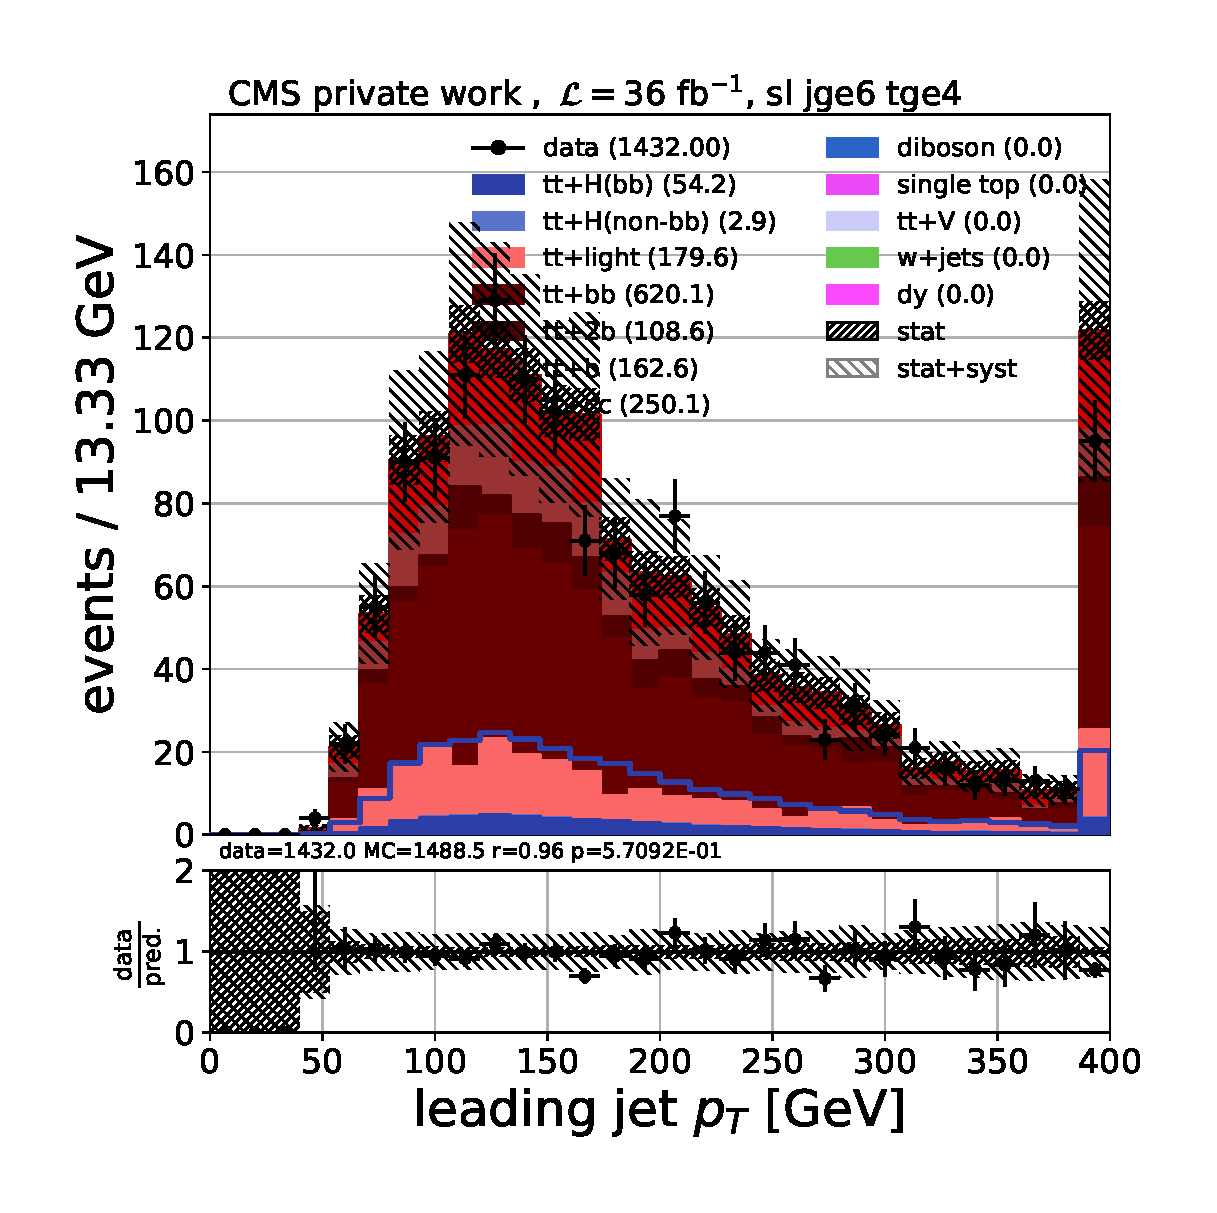
\includegraphics[width=0.4\textwidth]{figures/jetsByPt_0_pt.pdf}} 
\subfloat[fig 2]{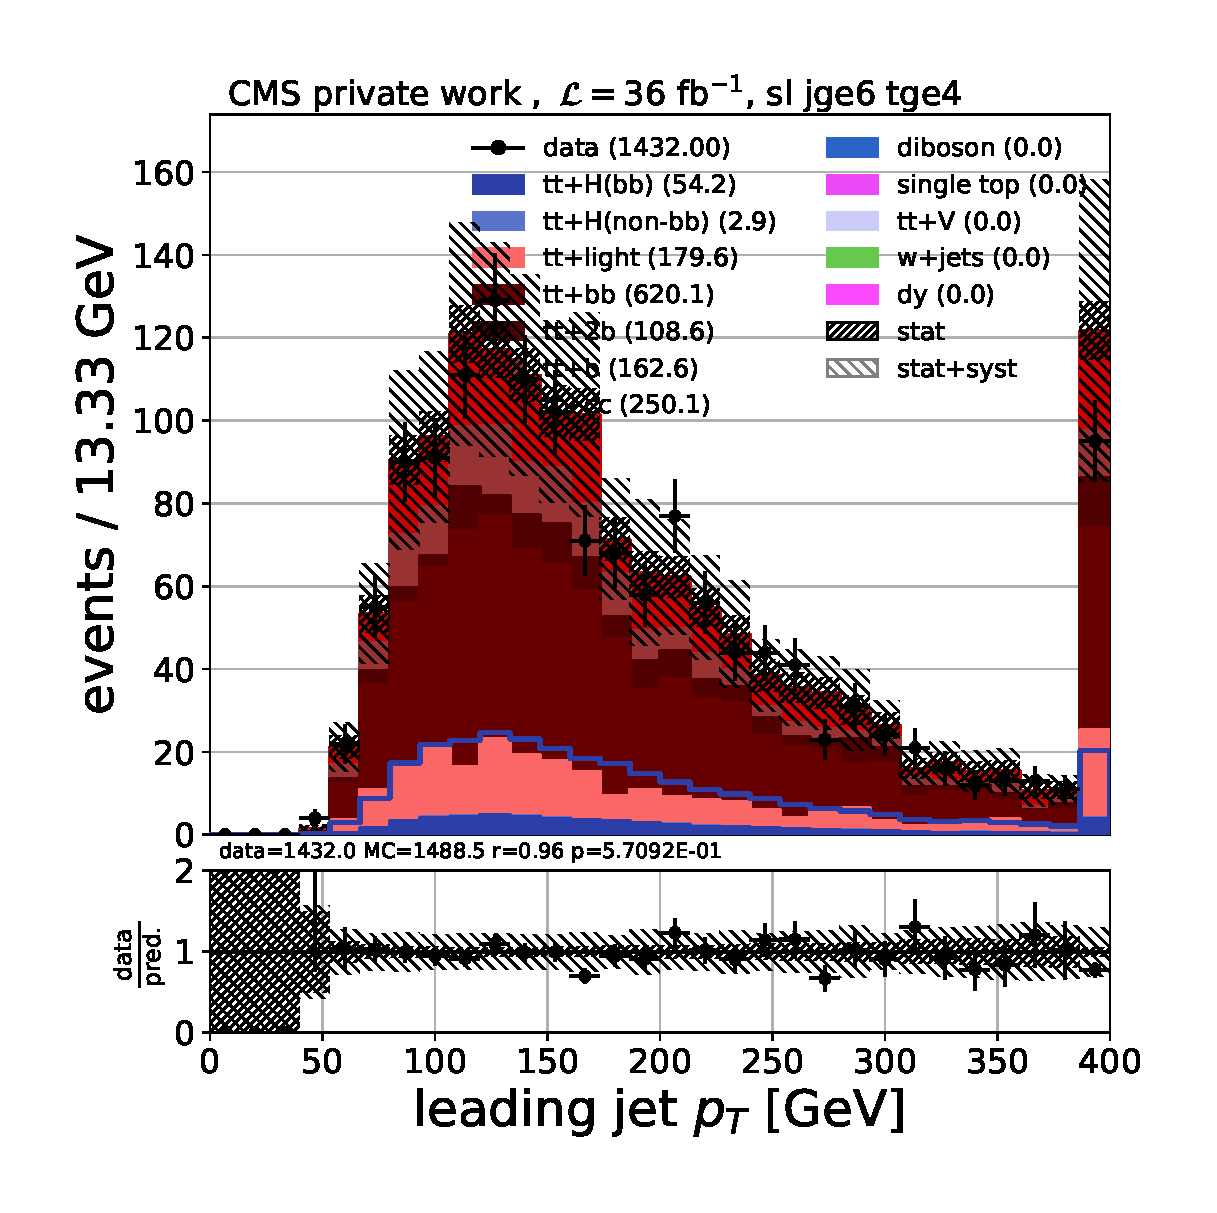
\includegraphics[width=0.4\textwidth]{figures/jetsByPt_0_pt.pdf}}\\
\caption{MEM assumptions.}
\label{fig:mem_assumptions}
\end{centering}
\end{figure}


\subsubsection{Integration}
\label{sec:mem_integration}

The MEM is implemented as a dedicated code in C++, relying on the \texttt{OpenLoops} C++ interface for the evaluation of the hard scattering amplitude. \texttt{ROOT} is used for numerical Lorentz algebra and \texttt{CLING} for interfacing the code to Python. The PDFs are evaluated using the \texttt{cteq66} set via the \texttt{LHAPDF} package. The numerical integration routines rely on the \texttt{VEGAS} algorithm that uses multiple passes to refine the integration grid, with the maximal number of evaluations tuned for approximately $<2.5 \dots 5\%$ numerical accuracy on the integral, suitable for use in a discriminator. We use the \texttt{CUBA} package for numerical integration, as it supports vector-valued integrands. The distribution of expected numerical accuracy is shown on \cref{fig:mem_numerical_accuracy} and illustrates the convergence of the numerical integration. Transfer functions can be provided in a flexible parametrisation using \texttt{ROOT}, however, as described in \cref{sec:mem_optimization}, we have also provided faster, optimized versions of the chosen Gaussian transfer functions. 

\fix Describe integration boundaries.

\begin{figure}
\begin{centering}
\subfloat[fig 1]{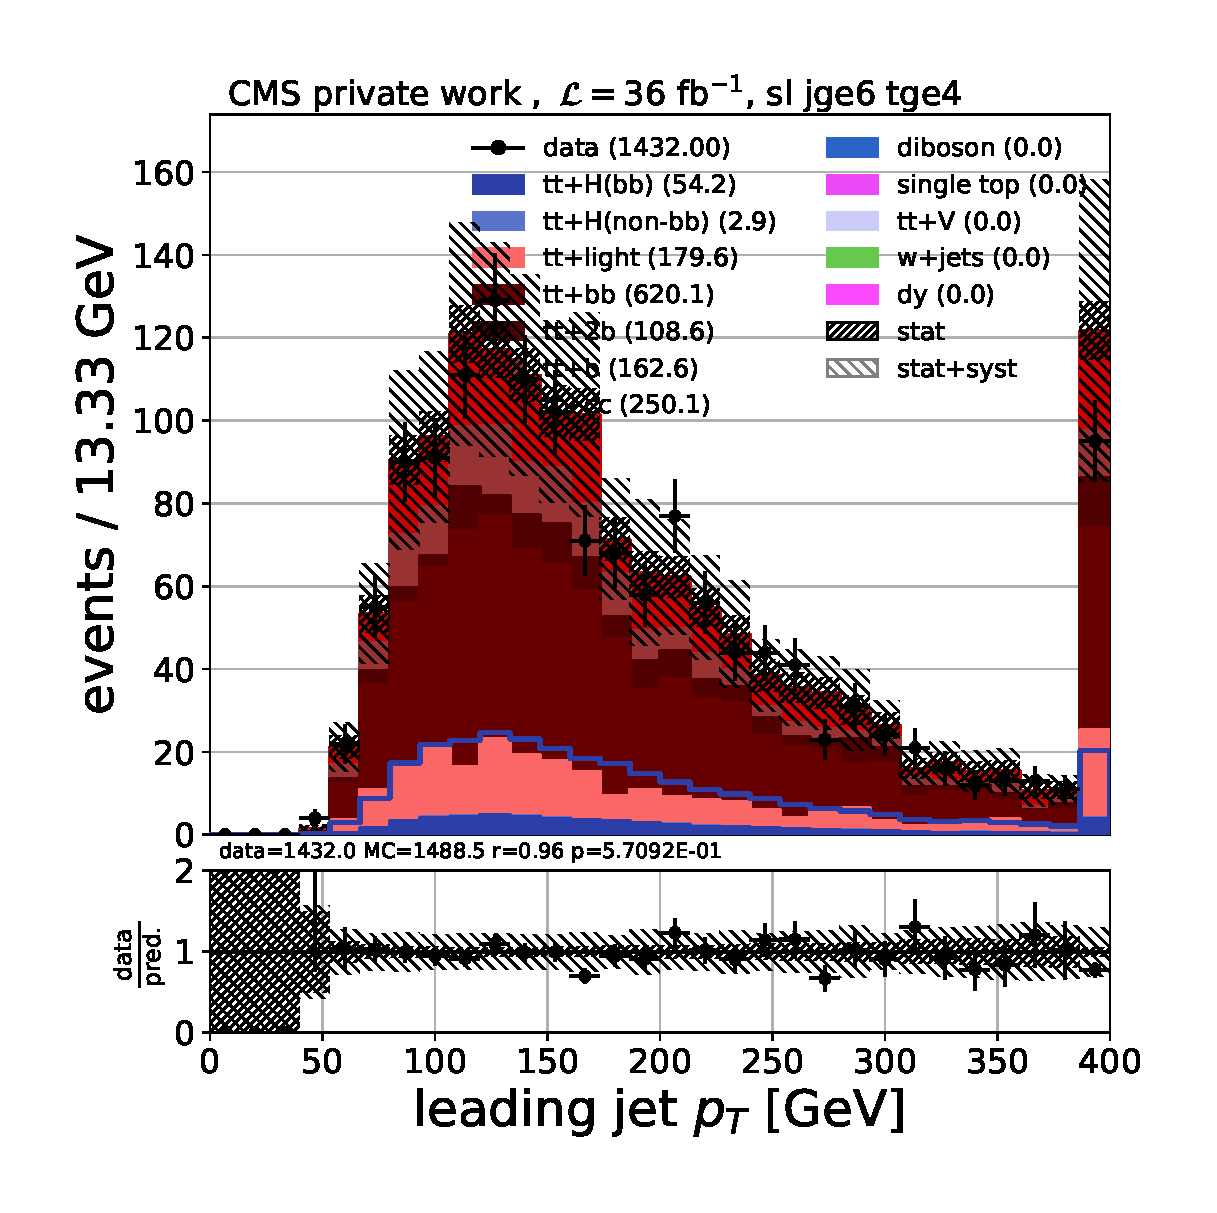
\includegraphics[width = 0.4\linewidth]{figures/jetsByPt_0_pt.pdf}} 
\subfloat[fig 2]{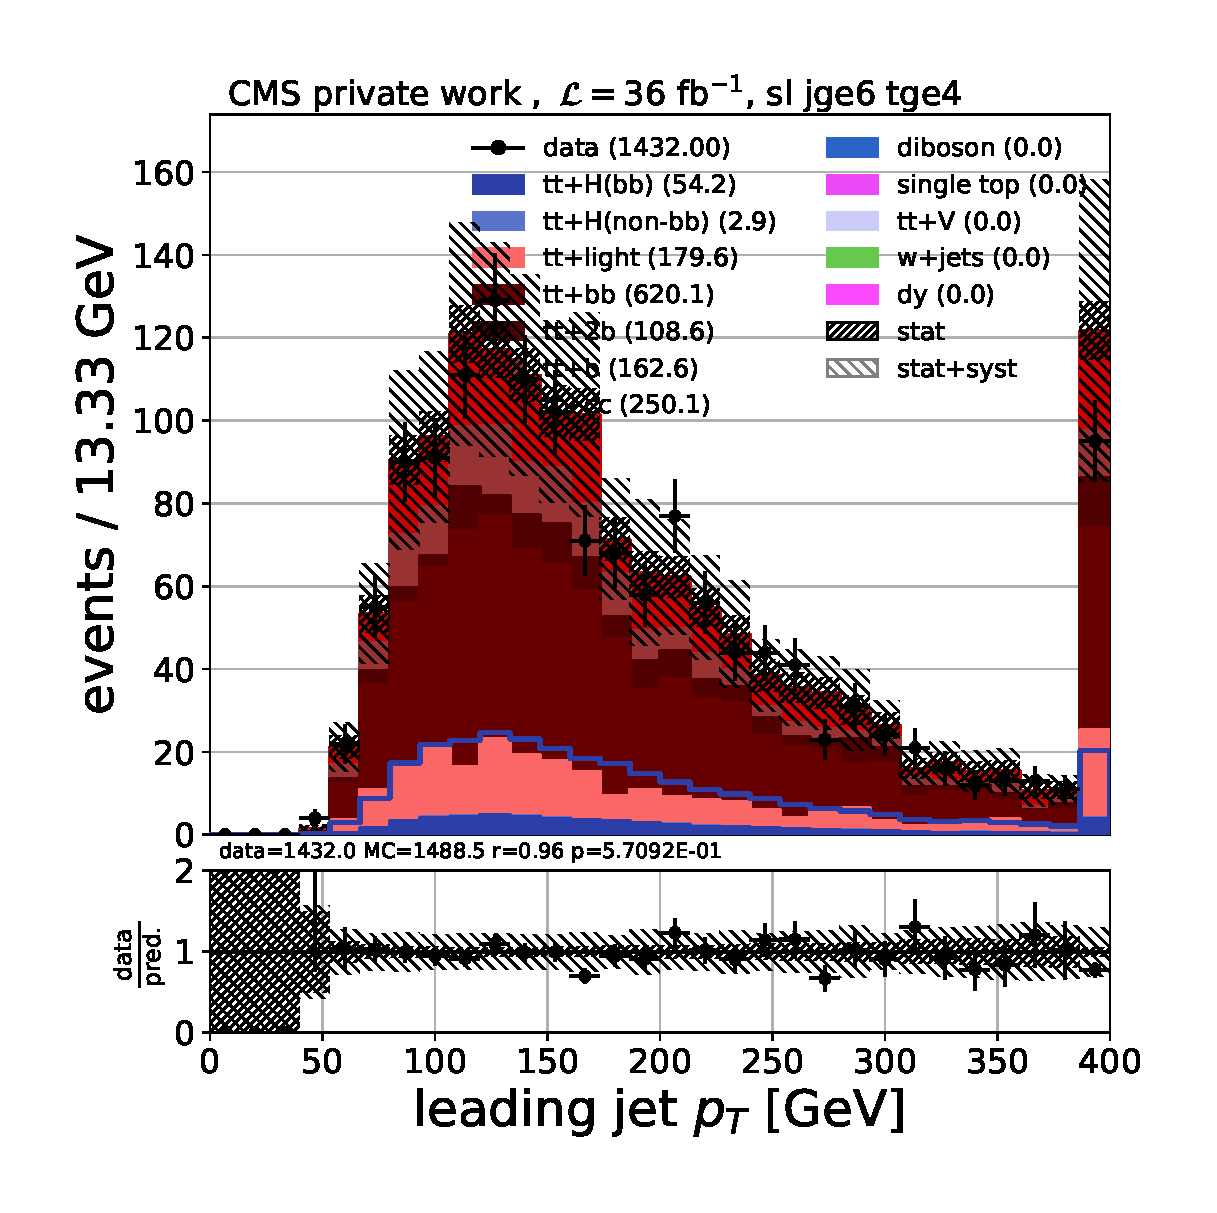
\includegraphics[width = 0.4\linewidth]{figures/jetsByPt_0_pt.pdf}}\\
\caption{MEM assumptions.}
\label{fig:mem_numerical_accuracy}
\end{centering}
\end{figure}

\subsubsection{Profiling and optimisation}
\label{sec:mem_optimization}

In order to optimize the MEM code, we have used the \texttt{igprof} sampling profiler tool to analyze the computational budget spent in various subroutines of the code. In general, we find    
that the overwhelming majority of time is spent within the integrand, out of which about 40\% is spent computing the transfer functions, 35\% is spent evaluating the scattering amplitude of the hard process, 10\% of computing the PDFs and about 10\% on manipulating the phase space volume. The evaluation of the transfer functions at a single phase space point is about an order of magnitude faster than the scattering amplitude. In order to achieve this ratio, we implemented the transfer functions explicitly as optimized C++ functions, instead of relying on a more generic approach using symbolic functions supported in ROOT. Additionally, as we have seen that a large part of time optimising the integration grid is spent in the exponential tails of the transfer function, we have used a piecewise exponential function that is suppressed far in the tails.

Currently, the MEM algorithm as implemented here can only be run on standard x86 CPU architectures. Although it has been shown that GPUs may offer strong parallelization benefits in evaluating the integral, it would be necessary to completely port and optimize the \texttt{OpenLoops} toolset on the GPU in a significant engineering effort\cite{Schouten:2014yza}, furthermore, GPU clusters are currently not commonplace in the WLCG.

\subsubsection{Computational budget}
\label{sec:mem_computational}
In this section, we present a feasibility estimation on using the MEM in a Run II analysis. This is necessary in order to predict the amount of computing resources that will be required. The computing time depends strongly on the number of permutations and integration variables needed for a given interpretation and event topology, as well as the total number of MC simulated events that are needed for the analysis.

\begin{table}[h!]
\begin{center}
\caption{The CPU budget of the MEM. \fix}
\label{tab:mem_cpu_budget}
\begin{tabular}{ccccc}
\hline
category & interpretation & average time & events & total \\
\hline
$1\ell6\mathrm{j}4\mathrm{t}$ & $2_{\mathrm{W}} 2_{\mathrm{h}} 2_{\mathrm{t}}$ & 60 CPUs/ev & 12044 ev & 100 CPUh \\
$1\ell7\mathrm{j}4\mathrm{t}$ & $2_{\mathrm{W}} 2_{\mathrm{h}} 2_{\mathrm{t}}$ & 60 CPUs/ev & 12044 ev & 100 CPUh \\
$1\ell\ge8\mathrm{j}4\mathrm{t}$ & $2_{\mathrm{W}} 2_{\mathrm{h}} 2_{\mathrm{t}}$ & 60 CPUs/ev & 12044 ev & 100 CPUh \\
$1\ell\ge5\mathrm{j}4\mathrm{t}$ & $1_{\mathrm{W}} 2_{\mathrm{h}} 2_{\mathrm{t}}$ & 60 CPUs/ev & 12044 ev & 100 CPUh \\
$1\ell\ge4\mathrm{j}4\mathrm{t}$ & $0_{\mathrm{W}} 2_{\mathrm{h}} 2_{\mathrm{t}}$ & 60 CPUs/ev & 12044 ev & 100 CPUh \\

\hline
\hline
\end{tabular}
\end{center}
\end{table}

\subsubsection{Uncertainties}
\label{sec:mem_uncertainties}

When using the MEM in a realistic experimental analysis, we need to evaluate the effect of systematic uncertainties on the MEM. In general, uncertainties modify the observables $\vec{y} \rightarrow \vec{y}^*$, for example the jet energies may be modified by uncertainties in the jet energy scale calibration. The naive approach to estimate the sensitivity of the discriminator would be to recompute the MEM discriminator weights $P(\vec{y}) \rightarrow P(\vec{y}^*)$. However, this turns out to be impractical, since the number of individual variations that need to be considered can easily reach $\mathcal{O}(10^2)$ and it is not realistic or practical to expend two orders of magnitude more computational resources.
In order to improve the situation, we first note that the variations are generally small, such that $\vec{y}^* \simeq \vec{y} + \delta \vec{y}$. Therefore, the numerical integration described in section \cref{sec:mem_implementation} would be performed on almost the same phase space, with a very similar integration grid.

Furthermore, we see from \cref{eq:definition} that the observables enter the definition of the MEM probability primarily through the transfer functions $W(\vec{y} | \vec{p})$ and affect the integration volume only secondarily. The most computationally costly part in the integrand is the evaluation of the LO scattering amplitudes for the hard process. Therefore, if we can promote the integrand to a vector-valued quantity, such that
\begin{equation}
|\mathcal{M}(\vec{p})|^2 W(\vec{y} | \vec{p}) \rightarrow |\mathcal{M}(\vec{p})|^2  \begin{pmatrix}
  W(\vec{y} | \vec{p}) \\
  W(\vec{y} + \delta \vec{y}_1 | \vec{p}) \\
  \dots \\
  W(\vec{y} + \delta \vec{y}_n | \vec{p})
 \end{pmatrix},
\end{equation}
the integration of the nominal and variated weight can be performed in a single pass using a a grid optimised for the whole integration. We test this approach by comparing the variation evaluated using vector integration to the full computation. As we wish to estimate the sensitivity of the analysis to this uncertainty, it is sufficient if the approximated variation has the same magnitude and direction as the true variation.

Additional complexity is introduced due to variations in the uncertainties possibly changing the topology of the reconstructed final state, as scaling jet energies down may cause jets to migrate under the experimental threshold $p_{T\mathrm{cut}}$. In order to account for this, in case a particular variation $\vec{y} + \delta \vec{y}_n$ changes the reconstructed final state, the MEM is still recomputed from scratch.

\subsubsection{MEM on the WLCG}

From \cref{sec:mem_computational} it is apparent that it is necessary to compute the MEM on distributed systems in order to have a reasonable turn-around time for the analysis. Therefore, we have parallelized the workflow both on the level of a computing cluster using \texttt{grid-control} and the WLCG using \texttt{CRAB}. On the WLCG, we have thus been able to take advantage of CMS computing resources opportunistically and have demonstrated that the MEM as implemented here is able to run on a wide range of data centers on a planetary scale. For this, we relied on \texttt{CMSSW} to provide a consistent environment along with user-provided external dependencies such as \texttt{OpenLOOPS}. We integrated the MEM into a multi-step workflow that produced the final analysis data sets directly from CMS MiniAOD in a single pass. This way, we were able to benefit from load balancing using data locality in CMS and reduced the number of manual intermediate steps and data management which can be error prone.
% asdasd \ttH

\subsection{Expected performance}
We demonstrate the expected performance of the MEM on a MC simulation sample of \ttH and \ttbar+jets. First, on \cref{fig:mem_proba}, we verify that the signal and background probabilities indeed behave as expected on their respective MC simulations.

\begin{figure}
\begin{centering}
\subfloat[MEM probability for the \ttH hypothesis.]{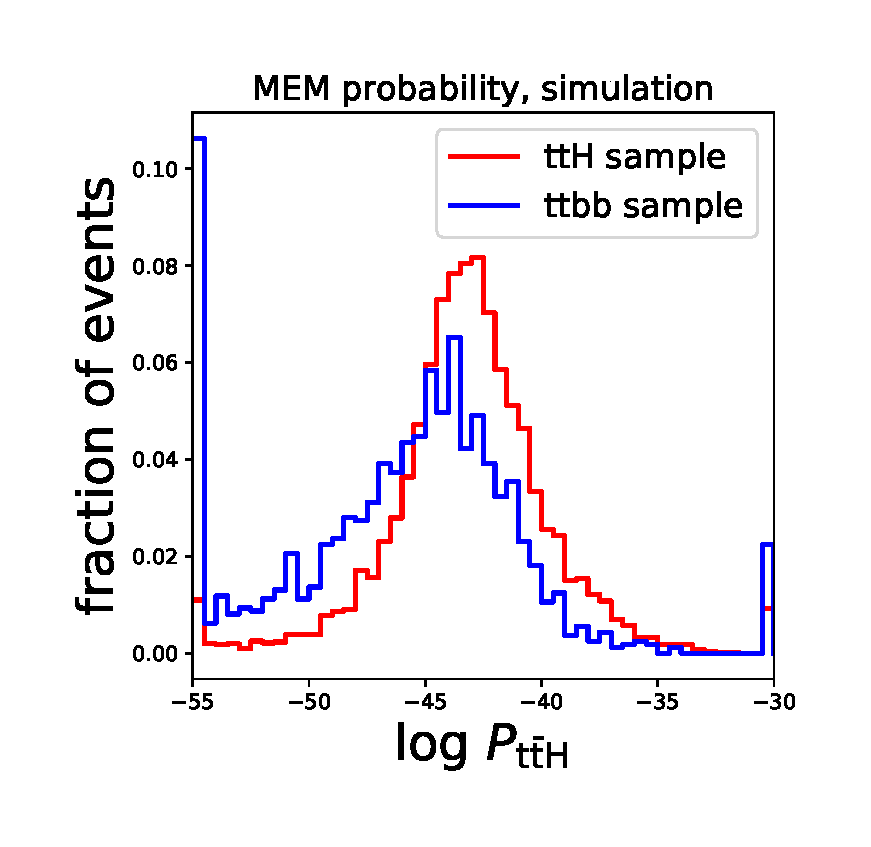
\includegraphics[width = 0.5\textwidth]{figures/mem_proba_tth.pdf}} 
\subfloat[MEM probability for the \ttbb hypothesis]{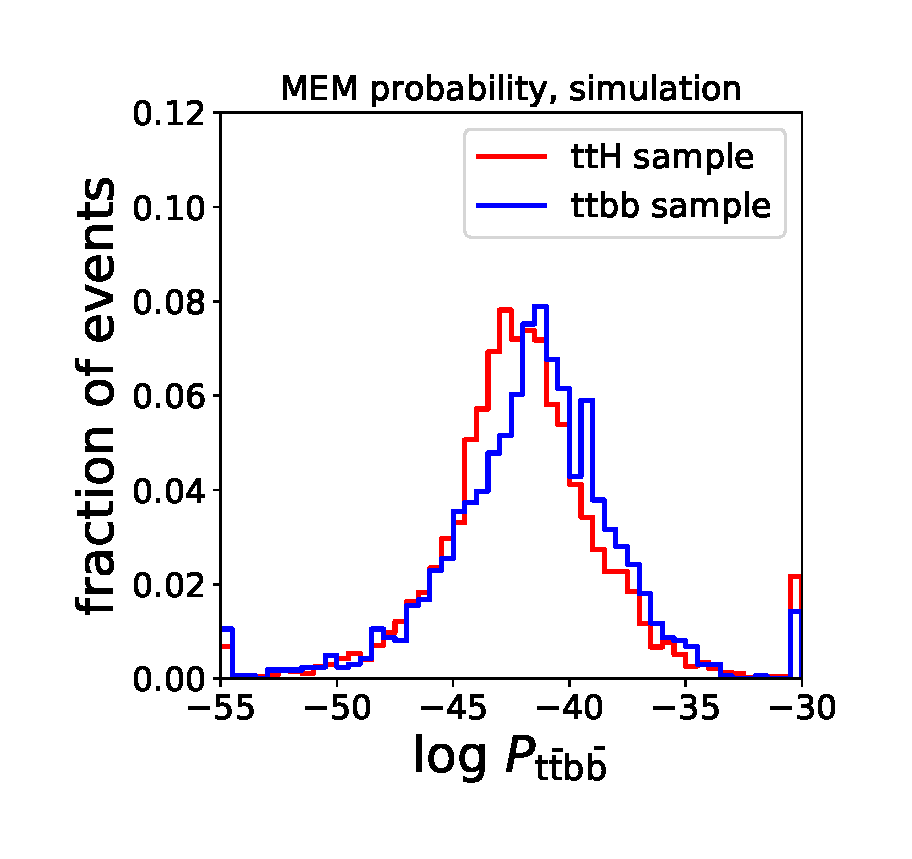
\includegraphics[width = 0.5\textwidth]{figures/mem_proba_ttbb.pdf}}\\
\caption{The expected distribution of the signal probability $P_{\ttHbb}$ and the background probability $P_{\ttbb}$ on MC simulation. We see that for the signal sample, the signal probability is on average higher than the background probability, and vice versa for the background. Here, we have selected events with exactly 1 isolated lepton, at least 6 jets, out of which 4 must be b tagged. Furthermore, the jets are required to be matched to quarks from the corresponding hard interaction on generator level.}
\label{fig:mem_proba}
\end{centering}
\end{figure}

\begin{figure}
\begin{centering}
\subfloat[fig 2]{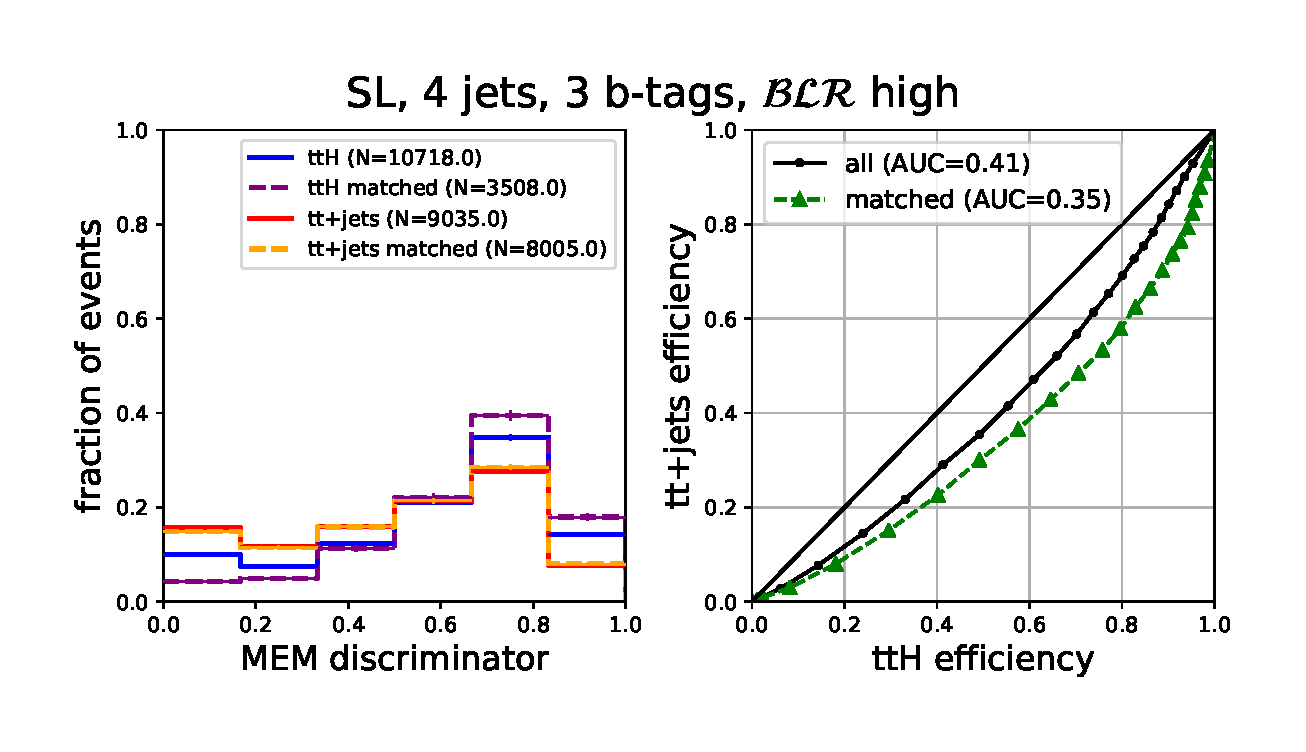
\includegraphics[width = 1.0\textwidth]{figures/mem_sl_j4_t3_blrH.pdf}}\\
\subfloat[fig 1]{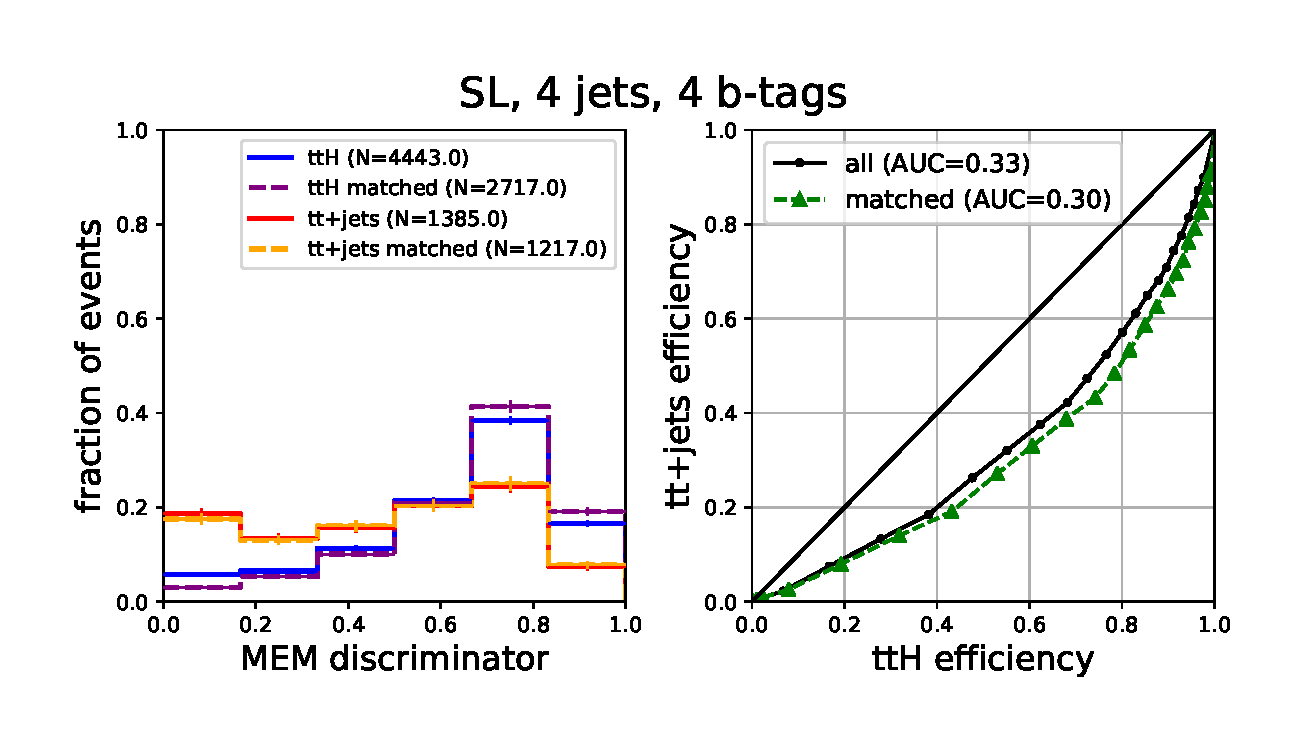
\includegraphics[width = 1.0\textwidth]{figures/mem_sl_j4_t4.pdf}}\\
\caption{Add your own figures before compiling}
\label{fig:some_example}
\end{centering}
\end{figure}

\begin{figure}
\begin{centering}
\subfloat[fig 2]{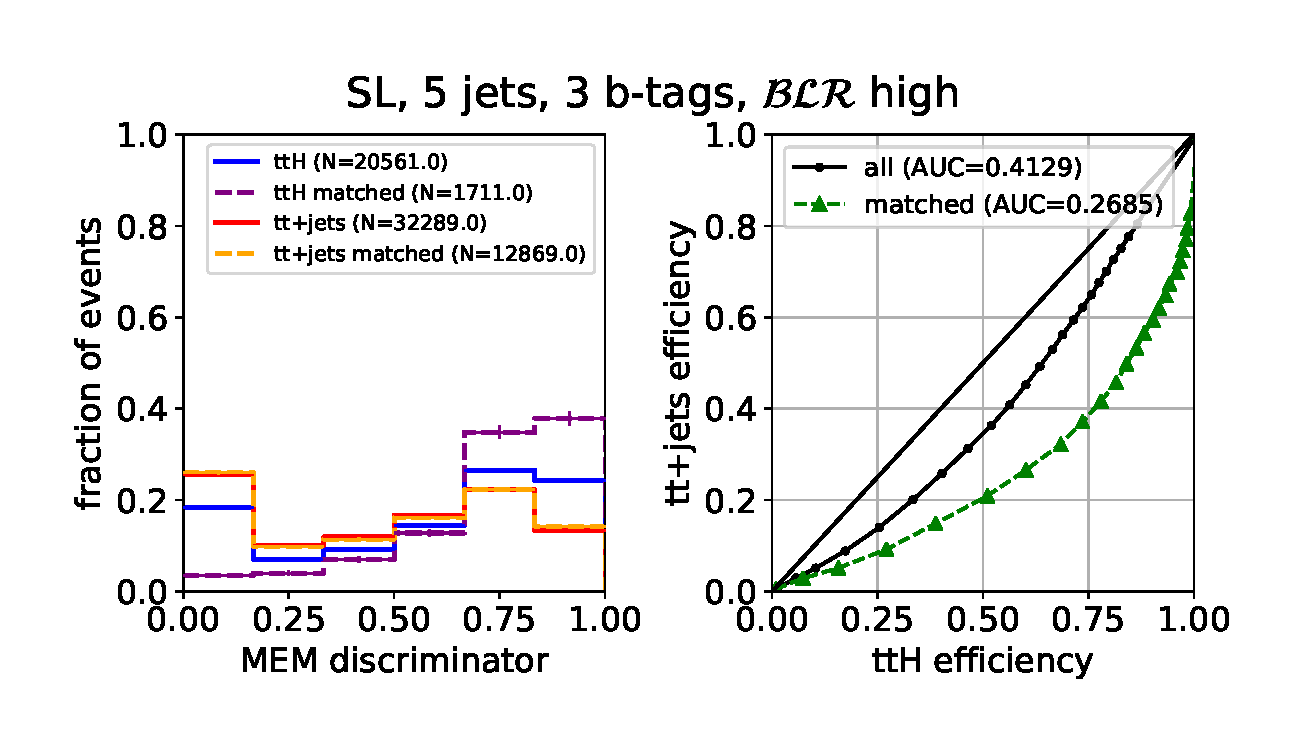
\includegraphics[width = 1.0\textwidth]{figures/mem_sl_j5_t3_blrH.pdf}}\\
\subfloat[fig 1]{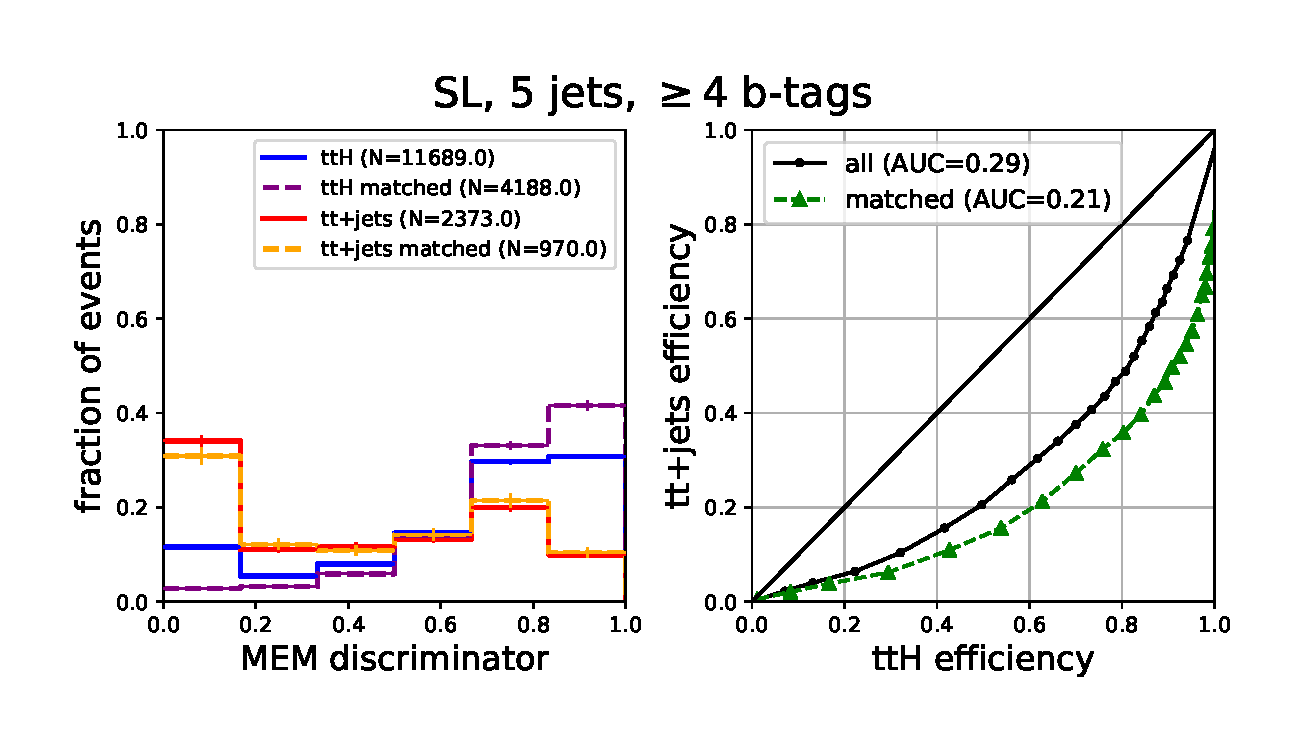
\includegraphics[width = 1.0\textwidth]{figures/mem_sl_j5_tge4.pdf}}\\
\caption{Add your own figures before compiling}
\label{fig:some_example}
\end{centering}
\end{figure}

\begin{figure}
\begin{centering}
\subfloat[fig 1]{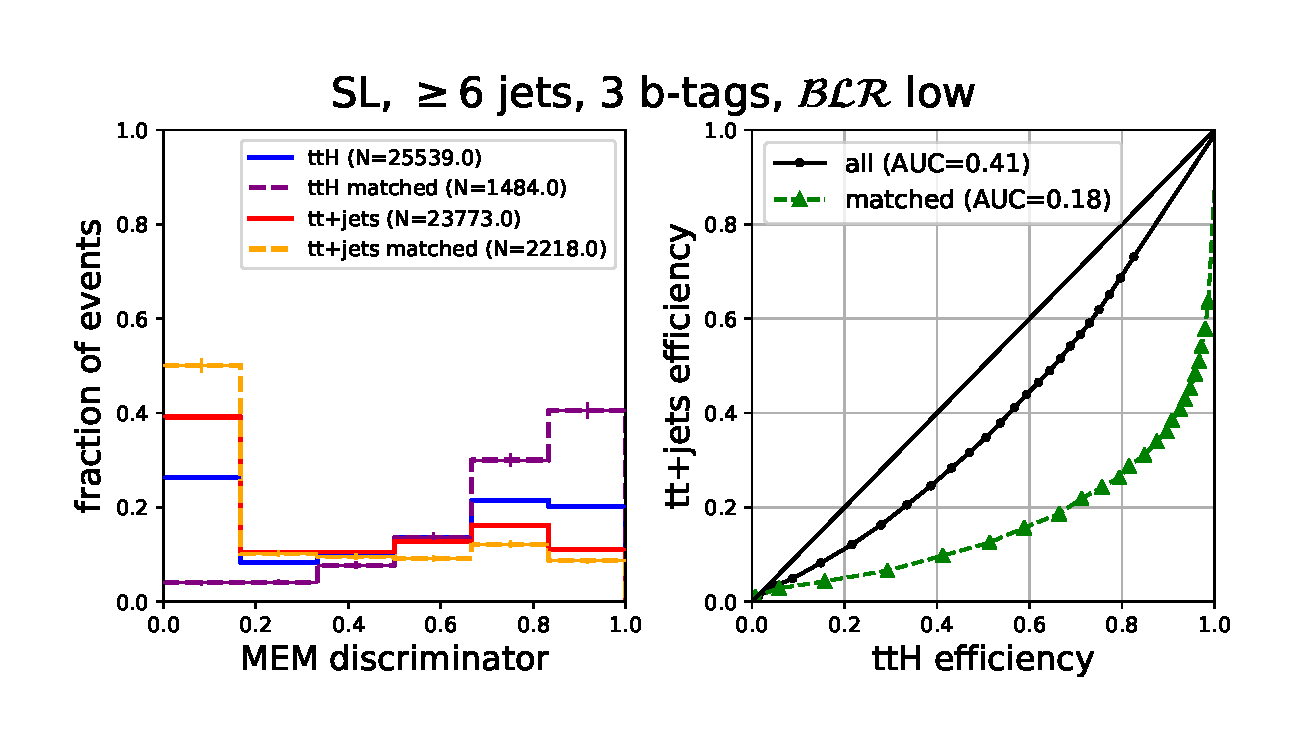
\includegraphics[width = 1.0\textwidth]{figures/mem_sl_jge6_t3_blrL.pdf}}\\
\subfloat[fig 2]{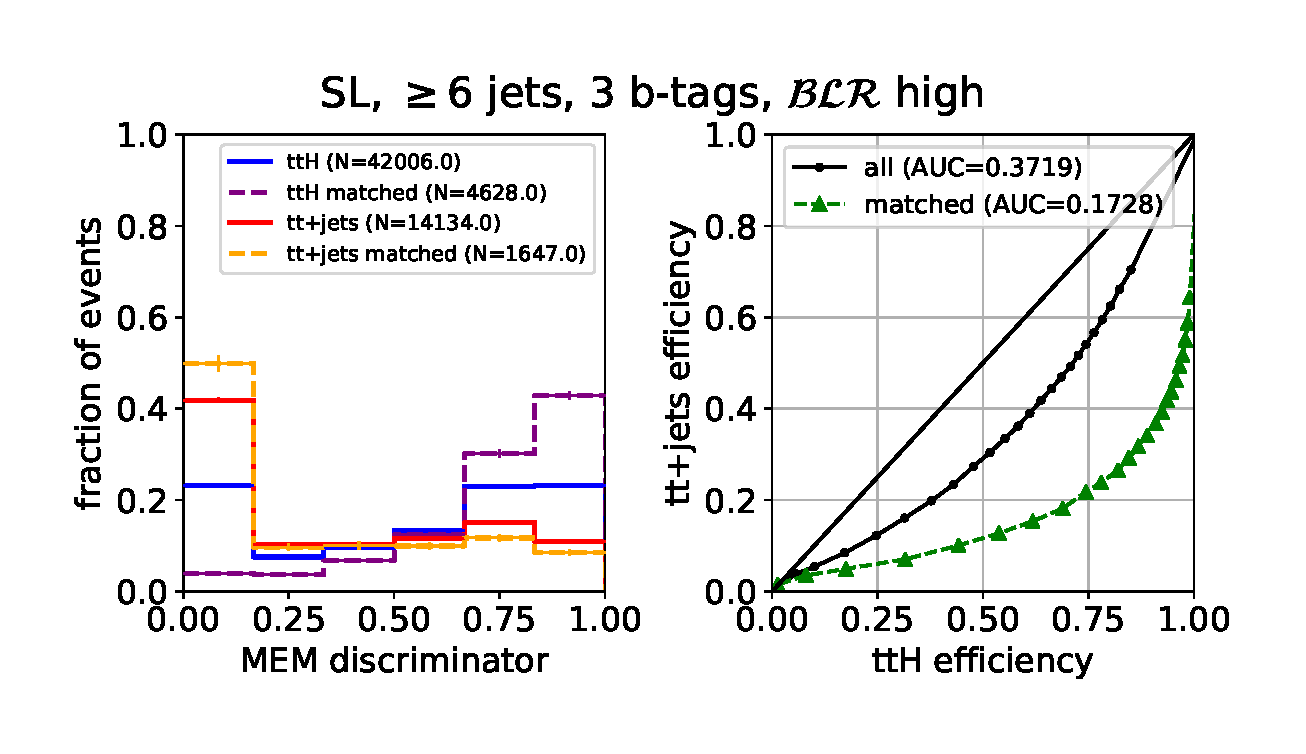
\includegraphics[width = 1.0\textwidth]{figures/mem_sl_jge6_t3_blrH.pdf}}\\
\caption{Add your own figures before compiling}
\label{fig:some_example}
\end{centering}
\end{figure}

\begin{figure}
\begin{centering}
\subfloat[fig 3]{\includegraphics[width = 1.0\textwidth]{figures/mem_sl_jge6_tge4.pdf}}\\
\subfloat[fig 4]{\includegraphics[width = 1.0\textwidth]{figures/mem_sl_jge7_tge4_7jet.pdf}}\\ 
\caption{Add your own figures before compiling}
\label{fig:some_example}
\end{centering}
\end{figure}


% \begin{figure}
% \begin{centering}
% \subfloat[fig 1]{\includegraphics[width = 0.4\linewidth]{figures/jetsByPt_0_pt.pdf}} 
% \subfloat[fig 2]{\includegraphics[width = 0.4\linewidth]{figures/jetsByPt_0_pt.pdf}}\\
% \subfloat[fig 3]{\includegraphics[width = 0.4\linewidth]{figures/jetsByPt_0_pt.pdf}}
% \subfloat[fig 4]{\includegraphics[width = 0.4\linewidth]{figures/jetsByPt_0_pt.pdf}} 
% \caption{Add your own figures before compiling}
% \label{fig:some_example}
% \end{centering}
% \end{figure}

% On \cref{fig:some_example} bla bla
%\section{Search for \ttHbb}

In this chapter, we will describe the search for \ttHbb using the MEM at the CMS experiment. This is based on preliminary results from CMS\cite{CMS-PAS-HIG-16-038} and ongoing work. We concentrate on the SL and DL decay channels of the top pair and the application of the MEM in the search for \ttHbb, where various subprocesses of \ttbar+jets are the primary irreducible background. Whenever we show results using CMS data, we use those plots and data that have been publicly released by the CMS collaboration.

Briefly, the analysis proceeds as follows. First, we select events with at least 1 (2) charged lepton(s) in the SL (DL) top decay channels and at least 4 jets, out of which 3 must be b tagged. The detailed identification criteria for the physics objects (jets and leptons) are motivated by established top quark analyses and are described in \cref{sec:object_id}. We then further divide the events into independent categories based on the jet and b tag multiplicity, described in \cref{sec:categories}. This is done in order to constrain the various subprocesses of \ttbar, described further in \cref{sec:ttbar_subprocesses}. In order to extract the signal strength $\mu$, we perform a combined template fit across all the categories, relying on the discriminating power provided by the MEM in categories with a high signal-to-background ratio and on other multivariate techniques in background-enhanced (control) regions. The fit is described in \cref{sec:statistical_method}.
A crucial component in the fit is the estimated systematic uncertainty, which drives the determination of the confidence interval of the estimated signal strength and is described in \cref{sec:systematics}. Throughout, we use MC simulation and data samples described in \cref{sec:data_mc}.

\subsection{Data and simulation}
\label{sec:data_mc}

We use proton-proton collision data collected by the CMS experiment at a center-of-mass energy of $\sqrt{s} = 13~\mathrm{TeV}$, corresponding to a total integrated luminosity of $12.9~\ifb$ in the SL channel and $11.4-12.9$ in the DL channel, denoted the CMS ICHEP2016 data set. The smaller amount of integrated luminosity for the DL channel is due to disabled $\mathrm{e}^+\mathrm{e}^-$ trigger paths disabled during data taking. We are currently working on publishing results with the full 2016 dataset of about $36~\ifb$, however, we cannot show the data before it is made public by the Collaboration.

We use MC generators to model the signal and background processes, interfaced to a parton shower and hadronization where appropriate. In order to model the detector effects, we use a detailed simulation of the reconstruction, selection efficiencies and detector resolutions based on \geant.

For the \ttH signal, \ttbar and single-top backgrounds, we use the NLO generator \powheg (v.2)\cite{Frixione2007,Re2011}. The use of an NLO model for the signal and main background modelling is a significant advancement over Run I analyses, where only a LO model was available. Besides \ttbar, we need to model the production of W or Z/$\gamma^*$ bosons with additional jets (denoted W/Z+jets or commonly V+jets), which are simulated using MADGRAPHATNLO (v. 2.2.2) and diboson production (WW, WZ, ZZ), simulated using \pythia (v. 8.2).

Throughout, we assume the value of the top quark mass to be $172.5\GeV/c^2$ and of the Higgs boson to be $125\GeV/c^2$. In order to describe the substructure of the protons via the parton density functions, we use the PDF parametrization provided by NNPDF3.0 and \pythia for showering and hadronization.

In order to model the production of hadrons, the parameters in the \pythia model have been tuned to historical Tevatron, LEP and LHC data\cite{CMS-PAS-GEN-14-001,Skands:2014pea}. In moving to $\sqrt{s} = 13~\TeV$, we have found that the default tune in \pythia does not reproduce the observed number of jets in data. Therefore, CMS has created a custom tune where the $\alpha_{\mathrm{ISR}}$, which controls the amount of initial-state radiation, and $h_{\mathrm{damp}}$, which suppresses real emissions in \powheg, have been adapted to reproduce the spectrum of the number of jets observed at CMS\cite{CMS-PAS-TOP-16-021}. This has been done on $\sqrt{s} = 8~\TeV$ data and significantly improves the modelling of the jet multiplicity.

We list the details of the MC samples in \cref{tab:mc_samples} and of data in \cref{tab:data_samples}.

\begin{table}[h!]
\begin{center}
\caption{The MC samples.}
\label{tab:mc_samples}
\begin{tabular}{cccc}
\hline
sample & generator & events & cross-section \\
\hline
\ttHbb & \powheg (NLO) and \pythia & 100k & 123 pb \\
\ttHnonbb & \powheg (NLO) and \pythia & 100k & 123 pb \\
\ttbar & \powheg (NLO) and \pythia & 100k & 123 pb \\
\hline
\hline
\end{tabular}
\end{center}
\end{table}

\begin{table}[h!]
\begin{center}
\caption{The data samples.}
\label{tab:data_samples}
\begin{tabular}{cccc}
\hline
trigger & run period & integrated luminosity \\
\hline
SingleMuon & Run B & $12.9~\ifb$ \\
\hline
\hline
\end{tabular}
\end{center}
\end{table}

In order to compare simulation to data, the simulated events are weighted according to the integrated luminosity and the predicted cross sections, which are taken from inclusive calculations. In particular, the \ttH cross section is known at NLO accuracy\cite{Dittmaier:1318996,Beenakker:2001rj,Beenakker:2002nc,Dawson:2002tg,Dawson:2003zu}. The Higgs boson branching fraction for \Hbb is affected by radiative corrections that are known up to N4LO (QCD) and NLO (EWK), resulting in an uncertainty of about 1-2\% \cite{Djouadi:1997yw,Butterworth:2010ym,deFlorian:2016spz}.
The cross section for \ttbar is know at NNLO accuracy and includes soft gluon resummation to NNLL\cite{Czakon:2011xx}. The cross-sections of the minor backgrounds are known to at least NLO, as summarized in \cref{tab:mc_samples}.

In addition to the hard interaction and the consequent showering and hadronization, events from additional pp interactions within the same bunch crossing are superimposed on the simulated event for all processes. The multiplicity distribution of these additional pileup events is reweighted to match the observed number of interactions in data. Furthermore, we correct the MC simulation with additional data-driven correction factors for b tagging, lepton efficiencies, described in \cref{sec:systematic_unc}.

\subsubsection{Modelling of \ttbar}
\label{sec:ttbar_subprocesses}
We subdivide the \ttbar sample further based on the generator-level flavor of additional jets, as the theoretical uncertainties of these subprocesses are uncorrelated and therefore need to be treated separately. In particular, we distinguish between
\begin{itemize}
\item \ttbb, where two additional bottom jets are created from one or more B hadrons,
\item \ttb with only one additional bottom jet,
\item \tttwob where jets from two B hadrons merge to produce one resolved bottom jet,
\item \ttcc if there are no additional bottom jets and at least on charm jet,
\item \ttlf in case there are no bottom or charm jets.
\end{itemize}
Despite considerable advances in theoretical modelling, the theoretical uncertainties in \ttbar + heavy flavour production are still significant\cite{Cascioli:2013era}. The aim of this splitting is to have an experimental way of constraining uncertainties on the various \ttbar~subprocesses.

The jet flavour is assigned using so-called \textit{ghost clustering}, where simple geometrical matching between partons and jets is superceded by clustering the partons and hadrons along with the jet constituents using standard jet algorithms. Furthermore, information from the generator-level decay chain is used assign the flavour of the jet according to the parton that gave rise to that jet\cite{Bartosik:2047049}.

\subsection{Event reconstruction and object identification}
\label{sec:object_id}
We use particle-flow to reconstruct events from particle candidates based on signals from all sub-detectors. This allows us to perform the analysis at the level of physics objects, namely, jets and leptons\cite{cms_particleflow:2017}. In order to mitigate the effects of pileup, we identify the primary vertex associated with the hard interaction by requiring $n_{\mathrm{dof}} > $, $|z| < 24~\mathrm{cm}$ and $|rho|<2~\mathrm{cm}$. The charged hadrons that are associated to pileup vertices are not included in the subsequent event reconstruction \cite{CMS:2014ata}.

Our final state of interest contains charged leptons ($\mathrm{e}^\pm$, $\mathrm{\mu}^\pm$), jets from light quarks and bottom quarks and \MET. This is due to the decay of the top quark, which in the standard model happens almost exclusively through $\mathrm{t} \rightarrow \mathrm{W} \mathrm{b}$.

\subsubsection{Charged leptons}
\label{sec:object_id_lep}

The leptonic decay of at least one of the W-bosons is required in order to pass the trigger selection. In order to suppress leptopns from the multi-jet QCD background, the charged leptons are required to be sufficiently isolated from hadronic activity using an isolation variable, which is computed within a cone of radius $\Delta R$ around the lepton direction (defined by the track) from the primary vertex as shown in \cref{eq:iso_mu} for muons and \cref{eq:iso_el} for electrons. In order to evaluate the isolation, we sum over the transverse momenta of all particle candidates ($p_T^{c.h.}$ for charged hadrons, $E_T^{n.h.}$ for neutral hadrons, $E_T^{\gamma}$ for photons) excluding the lepton itself and subtracting the neutral component from pileup events based on either the average pile-up energy ($\rho$) and effective area ($A$) for electrons or pile-up associated charged hadrons for muons. The prefactor $1/2$ for the pile-up component for muons is used to account for the approximate charged-to-neutral fraction in the hadronization of pile-up interactions\cite{CMS:2012}.

Furthermore, in order to supress leptons from non-prompt decays, we apply identification criteria based on various reconstruction parameters on the leptons. For muons, we apply the tight ID, which is a cut-based selection that suppresses decays in flight and is based on properties of the global track fit, number of hits in the pixel detector, tracker and muon chambers and sufficient proximity to the primary vertex\cite{Chatrchyan:2012xi,CMS:2017_muon_pog}. For electrons, the ID is based on a multivariate discriminator combining track-to-cluster matching observables, supercluster structure and cluster shapes \cite{Khachatryan:2015hwa,CMS:2017_egamma_pog}.

We summarize the lepton selection criteria in all the considered channels in table \cref{tab:lepton_selection} and describe the event selection further in \cref{sec:event_selection}.

\begin{equation}
\label{eq:iso_mu}
\mathrm{Iso}_{\mathrm{\mu}} = \sum_{\Delta R < 0.4} p_T^{c.h.} + \mathrm{max}\biggl(0, \sum_{\Delta R < 0.4} [E_T^{n.h.} + E_T^{\gamma} - \frac{1}{2} p_T^{\mathrm{PU}}] \biggr)
\end{equation}

\begin{equation}
\label{eq:iso_el}
\mathrm{Iso}_{\mathrm{e}} = \sum_{\Delta R < 0.3} p_T^{c.h.} + \mathrm{max}\biggl(0, \sum_{\Delta R < 0.3} [E_T^{n.h.} + E_T^{\gamma} - \rho A(\eta)] \biggr)
\end{equation}

\begin{table}[h!]
\begin{center}
\caption{The selection and ID criteria for the charged leptons.}
\label{tab:lepton_selection}
\begin{tabular}{c|ccccc}
\hline
channel & trigger & offline $p_T$ & $|\eta|$ & isolation \\
\hline
$\mathrm{\mu}^\pm$ & $p_T > 22\GeV$ & $p_T > 25\GeV$ & $|\eta| < 2.1$ &  $\mathrm{Iso}/p_T < 0.15$ \\

$\mathrm{e}^\pm$ & $p_T > 27\GeV$ & $p_T > 30\GeV$ & $|\eta| < 2.1$ & $\mathrm{Iso}/p_T < 0.15$\\

$\mathrm{e}^\pm\mathrm{e}^\mp$ & $p_T > 23 (12)\GeV$ & $p_T > 25 (15)\GeV$ & $|\eta| < 2.1$ & $\mathrm{Iso}/p_T < 0.15$\\

$\mathrm{e}^\pm\mathrm{\mu}^\mp$ & $p_{T} > 23_{\mathrm{e}} (8_{\mathrm{\mu}})\GeV$ & $p_T > 25 (15)\GeV$ & $|\eta| < 2.4$ & $\mathrm{Iso}/p_T < 0.25_{\mathrm{\mu}} (0.15_{\mathrm{e}})$ \\

$\mathrm{\mu}^\pm\mathrm{e}^\mp$ & $p_{T,} > 23_{\mathrm{\mu}} (8_{\mathrm{e}})\GeV$ & $p_T > 25 (15)\GeV$ & $|\eta| < 2.4$ & $\mathrm{Iso}/p_T < 0.25_{\mathrm{\mu}} (0.15_{\mathrm{e}})$ \\

$\mathrm{\mu}^\pm\mathrm{\mu}^\mp$ & $p_T > 17 (8)\GeV$ & $p_T > 25 (15)\GeV$ & $|\eta| < 2.4$ & $\mathrm{Iso}/p_T < 0.25$ \\

\hline
\hline
\end{tabular}
\end{center}
\end{table}

\subsubsection{Jets}
\label{sec:object_id_jets}
As the signal process is expected to produce between 4 to 6 jets at the leading order, an accurate reconstruction of jets is critical for this analysis. We use the anti-$k_T$ clustering algorithm\cite{Cacciari:2008gp} in the \texttt{FASTJET} implementation\cite{Cacciari:2011ma} with a distance parameter 0.4 to reconstruct jets from particle flow candidates \cite{CMS:2010xta,CMS:2009nxa,CMS:2010byl} and use the CMS PF jet ID algorithm to reject reconstruction failures and noise. The noise rejection works on the basis of cuts on jet energy fractions from various types of PF candidates, namely muons, electrons, photons, charged hadron and neutral hadron candidates and has a noise rejection of around 99\% \cite{CMS:2017wyc}.

Charged particles from pileup interactions are removed from clustering via the process of charged hadron subtraction. As the CHS relies on the reconstruction of tracks and the association of charged hadrons to tracks, the procedure is applied within the tracker volume ($|\eta| < 2.5$). We choose the leading PV as the one that has the highest magnitude of total track transverse momentum squared ($\sum |p_T^{\mathrm{track}}|^2$), with the rest of the PVs passing certain quality criteria as subleading PVs. Charged hadrons that are associated to tracks that are compatible with subleading PVs are removed. The subtraction procedure reduces the amount of jets arising from pileup from about 20\% to 5\% in the tracker region and also improves the momentum resolution and angular resolution ($\Delta R \simeq 0.01$) of jets\cite{CMS:2014ata}.

The experimentally measured energies of the jets have to be calibrated in terms of jet energy scale and resolution in both data and simulation. This is done using jet energy corrections, which correct for offset energy from multiple interactions in the same bunch crossing (pileup), the detector response based on simulation, the residual differences between data and simulation based on well-understood channels such as dijet production, and the detector response to jet flavor. 

The presence of pileup interactions generates a diffuse energy component that results in an energy offset in the jets. This offset correction is estimated using simulation by comparing jets in a MC sample without pileup events to the same simulation overlayed with pileup, geometrically matching them to the same underlying jet on the generator level \cite{cms_jec_2017}. An additional scale factor between data and simulation is extracted from zero-bias data using the random cone method \cite{Chatrchyan:2011ds}.  

The detector response is defined as the ratio between the reconstructed jet and a geometrically matched particle-level jet: $R = \langle p_T \rangle / \langle p_{T,\mathrm{particle}} \rangle$. It is estimated using a detailed model of the detector geometry, alignment, calibration and electrongs, implemented in \texttt{GEANT4} in bins of particle-level jet momentum and reconstructed jet $\eta$. The corrections are able to bring the response to a deviation of approximately 1\% from unity based on simulations. A residual data to simulation correction scale factor is applied on data based on transverse momentum balance from dijet, $\mathrm{Z}/\gamma$+jets and multijet events. These relative corrections rely on comparing the jet under calibration (probe) to a reference object (tag) and are of the order of a few percent in the central region considered in this analysis \cite{Chatrchyan:2011ds,cms_jec_2017}.

The jet response to different flavors is estimated using simulation, comparing the response of jets associated with partons according to a geometric matching between \pythia and \herwig. The flavor response is generally within a few percent, with differences between the flavors arising from fragmentation, where gluons fragment the most into soft particles that may remain unreconstructed and thus have the lowest response, and particle composition, with the neutral hadronic component having the largest effect. The flavor corrections are validated in Z+b-jet data and the residual correction between data and simulation is found to be consistent with unity \cite{Chatrchyan:2011ds}.

In contrast to jet energy scale, which is known with a total uncertainty better than $3\%$ over the relevant phase space, the jet $p_T$ resolution is known to around $10-20\%$. The resolution can be determined using $p_T$ balance as for JEC, but measuring the width instead of the mean of the response distribution. Both $\mathrm{Z}/\gamma$+jet and dijet events are used to determine the JER response \cite{Chatrchyan:2011ds}. In the MEM, we also use the approximate jet resolution functions derived from simulation in order to account for detector effects in the phase space integral as explained in \cref{sec:mem_transfer}.

\subsubsection{B-tagging}
\label{sec:object_id_btag}

Since the \ttHbb~signal is characterized by the presence of 4 bottom quarks, the accurate identification of jets arising from the hadronization of bottom quarks is important in this analysis. We rely on the combined secondary vertex algorithm (CSVv2) \cite{Chatrchyan:2012jua} to identify b jets. The CSVv2 algorithm uses secondary vertex properties such as the impact parameter along with track-based lifetime information to create a robust combined discriminator $\xi$ optimized to distinguish between jets arising from bottom quarks and light quarks using supervised learning. In Run 2 of the LHC, the CSVv2 algorithm has been improved with a new vertex reconstruction algorithm, as well as using artificial neural networks instead of a likelihood method to combine the input variables, such that correlations are properly taken into account\cite{CMS-PAS-BTV-15-001}.

The threshold value of the discriminant, above which a jet is considered to be b tagged ($\xi > \xi_c$) is chosen such that the efficiency of misidentifying jets arising from light quarks (u,d,s) or gluons as b-jets would be sufficiently low (~$1\%$). This corresponds to the efficiency of $70\%$ of correctly identifying bottom quarks and of mis-identifying charm quarks around $20\%$ and is denoted the CSVv2 medium working point.

We further use the value of the per-jet discriminant $\xi$ to construct a per-event likelihood discriminator between the hypotheses that the event contained 4 bottom quarks ($4\mathrm{b}$) or 2 bottom quarks ($2\mathrm{b}$) as shown in \cref{eq:blr}. The sum is performed over all the combinations of associating $M$ jets out of $N$ to bottom quarks and the rest to light quarks and $\mathrm{b}_i$ ($\mathrm{l}_i$) refers to the $M$ ($N-M$) jets associated to bottom quarks (light quarks) in the $i$-th permutation. We have used $f(\xi_k | \mathrm{b})$ ($f(\xi_k | \mathrm{l})$), which is the probability density that the $k$-th jet has a discriminator value $\xi_k$ assuming that it originated from a bottom quark (light quark). These b tagging likelihoods $\mathcal{BL}(\vec{\xi} | M\mathrm{b})$ are then used to construct a likelihood ratio $\mathcal{BLR}(\vec{\xi})$ (\cref{eq:blr_ratio}) that is optimized to suppress the the \ttlf background in favour of the \ttHbb signal.

\begin{equation}
\label{eq:blr}
\mathcal{BL}(\vec{\xi} | M\mathrm{b}) = \sum_{i \in \mathrm{perm}} \biggl[ \prod_{k \in \mathrm{b}_i} f(\xi_k | \mathrm{b}) \prod_{k \in \mathrm{l}_i} f(\xi_k | \mathrm{l}) \biggr]
\end{equation}

\begin{equation}
\label{eq:blr_ratio}
\mathcal{BLR}(\vec{\xi}) = \frac{\mathcal{BL}(\vec{\xi} | 4\mathrm{b})}{\mathcal{BL}(\vec{\xi} | 4\mathrm{b}) + \mathcal{BL}(\vec{\xi} | 2\mathrm{b})}
\end{equation}

We estimate the performance of this variable in terms of \ttHbb vs. \ttlf discrimination in simulation. On \cref{fig:blr_discrimination}, we see that the $\mathcal{BLR}$ discriminant improves over a fixed cut of $\ge4$ jets passing the CSVv2 medium working point ($N_{\mathrm{CSVM}} \ge 4$) by about 50\% ($0.04\% \rightarrow 0.022\%$) in terms of background rejection at the same signal efficiency ($\simeq 7\%$).

Furthermore, we have studied the efficiency of $\mathcal{BLR}$ in correctly reconstructing the event for MEM. For this, we evaluated the fraction of events where the final jets can be correctly matched to quarks from the hard interaction as a function of $\mathcal{BLR}$. We see on \cref{fig:blr_matching} that the likelihood discriminator is positively correlated with events where all the quarks have been matched to jets, with around $50\%$ of bottom quarks from top decay, $40\%$ of bottom quarks from Higgs decay and around $20\%$ of the light quarks from the W boson decay have been reconstructed as jets at $\mathcal{BLR} \simeq 0.8$. Furthermore, we see a positive correlation between the likelihood discriminator and the probability that the highest-probability permutation in the sum in \cref{eq:blr} with the $4$ bottom quark hypothesis corresponds to the bottom quarks from top or Higgs decay. In other words, the likelihood discriminator successfully tags the bottom quarks on an event-by-event basis.

\begin{figure}
\begin{centering}
\subfloat[Simulated shape of the discriminant.]{\includegraphics[width=0.5\textwidth]{figures/blr_shape_btagCSV.pdf}} 
\subfloat[Expected performance of the discriminant.]{\includegraphics[width=0.5\textwidth]{figures/blr_roc.pdf}}\\
\caption{Simulated distribution and expected performance of $\mathcal{BLR}$ discriminant in the SL channel, requiring at least 4 good jets. On (\textbf{a}), we show the simulated shapes of the discriminant for signal (\ttHbb) and the various \ttbar+jets backgrounds. On (\textbf{b}), we compare the efficiency to select \ttHbb and \ttlf events. We see that the $\mathcal{BLR}$ discriminant compares favorably to a fixed cut on number of b tags. The cMVAv2 discriminator further improves the performance.}
\label{fig:blr_discrimination}
\end{centering}
\end{figure}


\begin{figure}
\begin{centering}
\subfloat[Fraction of events with correct matching.]{\includegraphics[width=0.5\textwidth]{figures/blr_matching.pdf}} 
\subfloat[Fraction of matched events with correct tagging.]{\includegraphics[width=0.5\textwidth]{figures/blr_matching_tag.pdf}}\\
\caption{Estimation of the fraction of events where the bottom quarks from the top quark, the Higgs boson and the light quarks from the W boson are reconstructed as jets in the final state on (\textbf{a}). We study the event-level b tagging efficiency on (\textbf{b}), where we plot the fraction of events where the highest-likelihood permutation correctly assigned the bottom quarks to jets with respect to all events where the quarks were reconstructed as jets without considering tagging.}
\label{fig:blr_matching}
\end{centering}
\end{figure}
 
The likelihood ratio as defined here ignores the differences in $f(\xi_k | \mathrm{b})$ and $f(\xi_k | \mathrm{c})$, meaning that in the case of $\mathrm{W} \rightarrow \mathrm{c}\bar{\mathrm{s}} (\bar{\mathrm{d}})$ decays, the discriminator is inoptimal. We have investigated extending this likelihood to also account for the possibility of such decays by a straightforward extension of $\mathcal{BL}(\vec{\xi} | M\mathrm{b}~1\mathrm{c})$. However, we have found that the additional combinatorial complexity suppresses any increased discrimination power and further progress in this would likely require methods that are better able to deal with the combinatorial problem using kinematic information.

We use this likelihood discriminant to define heavy-flavour enhanced regions, as well as to select the bottom quark candidates in the application of the MEM, as described in \cref{sec:mem_application}. 

As we have used the detailed b tagging discriminator shape information in constructing the $\mathcal{BLR}$, we must experimentally calibrate the full range of this observable using data. This is done by deriving a scale factor between data and simulation that depends on the discriminator value, jet kinematics and flavour using a tag-and-probe method. The tag jet is required to pass the medium operating point that has been described earlier and iteratively correcting the discriminator distribution of the probe jet. In order to extract the weight for the b jets, the procedure relies on dilepton \ttbar events with the contribution from light jets and backgrounds subtracted using simulation, whereas for the scale factor for light jets, Z+jets events are used. The procedure is iterative, as the scale factor for light jets is required for the extraction of the b jet scale factor and vice versa \cite{CMS:2013sea,CMS-PAS-BTV-15-001}. The systematic uncertainties from this reweighting are described in \cref{sec:systematic_unc}.

The leptonic decays of the W boson produce neutrinos, which are only partially reconstructed by the detector as \MET, defined as the negative sum of all the momenta of the reconstructed particles in the transverse plane. In the SL channel, we can directly associate the \MET with the transverse momenta of the neutrinos, through the modelling of the recoil as described in \cref{sec:transfer_functions} whereas in the DL channel, only the total momentum of both neutrinosis  constrained by the \MET.

\subsection{Event selection and categorization}
\label{sec:event_selection}

First, the large multi-jet QCD background is reduced to negligible levels by requiring that at least one of the top quarks in \ttHbb decays leptonically. We divide events to two exclusive lepton categories: SL and DL, based on the multiplicity of the reconstructed charged leptons passing the quality cuts described in \cref{sec:object_id_lep}. This is achieved by vetoing events with any additional leptons passing loosened quality criteria. For the dilepton category, we further suppress the Drell-Yan background by requiring $m_{\ell\ell} > 20\GeV$ and Z+jets by rejecting events with $76\GeV < m_{\ell\ell} < 106\GeV$. Furthermore, the leptons are required to have opposite charge. In the DL same-flavour channels, we require $\MET > 40\GeV$. We do not explicitly distinguish between cases where the top quark decays to $\mathrm{\tau}$ leptons, although these events can still pass the selection in case the $\mathrm{\tau}$ decays leptonically.

Events from \ttHbb have a large number of jets and b tags compared to the V+jets backgrounds. Therefore, we require the presence of at least 4 jets passing the quality criteria (\cref{sec:object_id_jets}), out of which at least 2 must be b tagged according according to the medium working point (\cref{sec:object_id_btag}). This brings us to the \ttbar dominated region, where we further distinguish between 7 categories in the SL channel
\begin{itemize}
\item $\ge 6~\mathrm{jets},\ge 4~\mathrm{b~tags}$; $ 5~\mathrm{jets},\ge 4~\mathrm{b~tags}$; $ 4~\mathrm{jets},4~\mathrm{b~tags}$, that are the most signal-enriched regions,
\item $\ge 6~\mathrm{jets},3~\mathrm{b~tags}$; $5~\mathrm{jets} 3,\mathrm{b~tags}$; $5~\mathrm{jets},3~\mathrm{b~tags}$, that contain a significant amount of \ttcc and \ttbb,
\item $\ge 6~\mathrm{jets},2~\mathrm{b~tags}$, that is \ttlf-enhanced and used to constrain JEC uncertainties,
\end{itemize}
and three categories in the DL channel
\begin{itemize}
\item $\ge 4~\mathrm{jets},\ge 4~\mathrm{b~tags}$,
\item $\ge 4~\mathrm{jets},3~\mathrm{b~tags}$,
\item $ 4~\mathrm{jets},2~\mathrm{b~tags}$,
\end{itemize}
resulting in a total of 10 exclusive categories.

We use the MEM as a \ttHbb to \ttbb discriminator in the categories with $\ge 4$ b tags as these are the primary signal-enriched regions. The categories with 3 b tags ar further subdivided into $\mathcal{BLR} \ge C$ (high) and $\mathcal{BLR} < C$ (low), where the high categories are enriched in \ttHbb and therefore will rely on the MEM for discrimination. The low-$\mathcal{BLR}$ categories are retained as control regions where we fit the jet b tagging discriminator. In the categories with 2 b tags, we fit the jet $p_T$ distribution in order to constrain the jet energy scale correction uncertainties. The value of $C$ is determined so that it would result in a signal acceptance of $\epsilon = 0.5$ and significantly lower background acceptance.

\subsection{Signal extraction}
\label{sec:mem_application}
The likelihood discriminant based on b tagging enhances the \ttbar + heavy flavour component, but the cross-section of \ttbb is still an order of magnitude larger that \ttHbb. Furthermore, we cannot directly reconstruct the resonant peak of the \Hbb~decay as a natural disciminant between the signal and non-resonant background. Even though the width of the SM Higgs boson is relatively small compared to detector resolution ($\Gamma = X~\GeV$), the presence of multiple additional bottom quarks due to top decay in the final state creates a combinatorial self-background in the form of an ambiguity in choosing the candidate jets for the \Hbb~decay.

An experimental mass estimator built from randomly selected jet pairs results in a much broader distribution compared to experimental resolution, whereas choosing the pair of jets that would give a mass closest to $m_H$ would cause also the background to exhibit a signal-like peak.

Therefore, we use the MEM discriminant, introduced in \cref{sec:mem}, to compute theory-motivated weights $P_{\ttHbb}$ and $P_{\ttbb}$ for each candidate event. We construct a discriminant based on the likelihood ratio of these weights,

\begin{equation}
\label{eq:mem_ratio}
P_{\mathrm{s}/\mathrm{b}} = \frac{P_{\ttHbb}}{P_{\ttHbb} + \alpha P_{\ttbb}}
\end{equation} 
which based on the Neyman-Pearson lemma, described in \cref{sec:test_statistic}, is the optimal test statistic between the signal and background hypotheses. The scale factor $\alpha$ is optimized to adjust the relative normalization of the signal and background probabilities and is introduced to allow the dynamic range of $P_{\mathrm{s}/\mathrm{b}}$ to be uniform in the range $P_{\mathrm{s}/\mathrm{b}} \in [0, 1]$. Adjusting this coefficient does not change the signal-to-background discrimination power of the discriminant as it is a monotonic rescaling, but allows us to discretize the distribution into a small number of bins without losing sensitivity.

As an improvement over the search for \ttHbb performed by the CMS experiment in Run I \cite{Khachatryan:2015ila}, we use the MEM discriminant also in categories which are not fully reconstructed, but still contain a large amount of signal, namely 5-jet and 4-jet categories in the SL channel. The details of the additional MEM hypotheses are described in \cref{sec:event_interpretation}. We list the discriminant that has been used in different categories in \cref{tab:cat_discriminant}. 


\begin{table}[h!]
\begin{center}
\caption{The analysis categories and the discriminators used in those categories.}
\label{tab:cat_discriminant}
\begin{tabular}{c|c}
\hline
category & discriminant \\
\hline
SL $\ge6$ jets, $\ge4$ tags & MEM SL $2_{\mathrm{W}} 2_{\mathrm{h}} 2_{\mathrm{t}}$ \\
SL $\ge6$ jets, $3$ tags, $\mathcal{BLR}$ high & MEM SL $2_{\mathrm{W}} 2_{\mathrm{h}} 2_{\mathrm{t}}$ \\
SL $\ge6$ jets, $3$ tags, $\mathcal{BLR}$ low & leading jet b discriminator \\
SL $\ge6$ jets, $2$ tags & leading jet $p_T$ \\
\hline
SL $5$ jets, $\ge4$ tags & MEM SL $1_{\mathrm{W}} 2_{\mathrm{h}} 2_{\mathrm{t}}$ \\
SL $5$ jets, $3$ tags, $\mathcal{BLR}$ high & MEM SL $1_{\mathrm{W}} 2_{\mathrm{h}} 2_{\mathrm{t}}$ \\
SL $5$ jets, $3$ tags, $\mathcal{BLR}$ low & leading jet b discriminator \\
\hline
SL $4$ jets, $\ge4$ tags & MEM SL $0_{\mathrm{W}} 2_{\mathrm{h}} 2_{\mathrm{t}}$ \\
SL $4$ jets, $3$ tags, $\mathcal{BLR}$ high & MEM SL $0_{\mathrm{W}} 2_{\mathrm{h}} 2_{\mathrm{t}}$ \\
SL $4$ jets, $3$ tags, $\mathcal{BLR}$ low & leading jet b discriminator \\
\hline
DL $4$ jets, $\ge4$ tags & MEM DL $2_{\mathrm{h}} 2_{\mathrm{t}}$ \\
DL $4$ jets, $3$ tags, $\mathcal{BLR}$ high & MEM DL $2_{\mathrm{h}} 2_{\mathrm{t}}$ \\
DL $4$ jets, $3$ tags, $\mathcal{BLR}$ low & leading jet b discriminator \\
DL $4$ jets, $2$ tags & leading jet $p_T$ \\
\hline
\hline
\end{tabular}
\end{center}
\end{table}

We use the \ttbb matrix element as a representative background in all cases. This gives the best separation in the most signal-rich categories against \ttbb and is further motivated by simulation, where we see that using this process as background still achieves a high rate of separation in categories enriched in other \ttbar+jets subprocesses. As a future improvement, considering additional background hypotheses in different categories is expected to improve the discrimination at the cost of computational complexity.

As the $\mathcal{BLR}$ method is optimized to identify the set of jets that are most compatible with arising from 4 bottom quarks, we further augment the MEM by assuming that the bottom quarks need to be considered only among those 4 jets, as explained in \cref{sec:event_interpretation}. This means that the we have exactly 4 candidates for the bottom quarks from \Hbb~and $\mathrm{t} \rightarrow \mathrm{W} \mathrm{b}$ decay, whereas the remaining jets are assumed to arise from $\mathrm{W} \rightarrow \mathrm{q} \mathrm{q}'$ or QCD radiation. 

In the next section, we will discuss the systematic uncertainties that affect the analysis.

\subsection{Systematic uncertainties}
\label{sec:systematic_unc}
We have already mentioned in passing that there are a number of experimental as well as theoretical uncertainties that must be taken into account.

Among the experimental uncertainties, the dominant ones are uncertainties on the jet energy scale corrections (\cref{sec:jec_unc}) and the reweighting of the b tagging discriminant (\cref{sec:btag_unc}). Both of these can affect the yields of all the processes, since they change the selection efficiency, as well as the shapes of the final discriminants. In case the source of the uncertainty is the same across several categories, the nuisance parameters associated with the uncertainties are treated as fully correlated.

From the theoretical uncertainties, the most important ones arise from the variation of the renormalization and factorization scale of the \ttbar+jets subprocesses and the \ttH signal. Furthermore, since the \ttbar+jets \texttt{POWHEG} model we currently use in the analysis treats the \ttbb process only at leading order accuracy, where the $\mathrm{b}\bar{\mathrm{b}}$ pair is generated from gluon splittings using a parton shower, we have considerable additional theoretical uncertainties on the modelling of \ttbb.

We give a detailed overview of the most important experimental and theoretical uncertainties along with their estimation in the next sections. The full list of systematic uncertainties along with their effect is show in \cref{tab:systematic_uncertainties}.

\begin{table}[h!]

\begin{center}
\caption{}
\label{tab:systematic_uncertainties}
\begin{tabular}{c|cccc}
\hline
uncertainty & normalization & shape & process & model \\
\hline
JEC (26 sources) & yes & yes & all & gaussian \\
btag & yes & yes & all & gaussian \\
\hline
bla & yes & yes & all & gaussian \\
\hline
\hline
\end{tabular}
\end{center}
\end{table}

\subsubsection{Jet energy correction uncertainties}
\label{sec:jec_unc}
In Run II, we consider various sources of jet energy correction uncertainties with their corresponding correlations, as opposed to a single bulk JEC uncertainty as was done for this analysis in Run I. This significant advancement has resulted from an improved modelling of the detector performance and better calibration techniques developed with more data. 

The magnitude and correlation of the uncertainties on jet energy scale and resolution are estimated in a dedicated CMS analysis and are provided as a vector of per-jet corrections with $p_T$ and $\eta$ dependent correlations. The most important groups of correction uncertainties are the following.
\begin{itemize}
\item Pileup offset, which results from from extra energy deposited in jets from additional pp interactions within the same bunch crossing (in-time pileup) or due to the finite signal decay time in the calorimeters (out-of-time pileup). The uncertainty for this source results from the $\eta$-dependent scale factor used to correct the offset distribution measured in simulation.
\item Relative $\eta$-dependent corrections, which calibrate the forward regions of the detector with respect to the central region. The uncertainties on this source arise from jet energy resolution and from the modelling of ISR+FSR.
\item Uncertainties on the absolute energy scale, which are derived using Z/$\gamma$+jet and multijet data. The energy scale uncertainties are driven by the muon momentum scale and the single pion response in the HCAL. Furthermore, the uncertainties in fragmentation are assessed in a comparison of \texttt{PYTHIA} and \texttt{HERWIG++}.
\item Uncertainties in the modelling of the detector response for jet flavor, which are assessed using simulation and are largest for gluon jets.
\item Finally, due to radiation damage, there is a residual time-dependent uncertainty in the scale corrections, which is estimated using dijet events in different run periods.
\end{itemize}
These 5 groups factorize into about 26 independent sources with up and down variations.

In order to account for the JEC scale uncertainties in the analysis, we propagate the uncertainties in jet energy corrections and resolution to the jet momenta and all the event-level observables that derive from them in MC by shifting the jet energy scale by one standard deviation. This is done separately for all the sources so that we can fully account for the correlations between the various sources. Thus, we are able to account for both the changes in efficiency (normalization) and discriminator shape in the final analysis categories.
In order to propagate the uncertainty to a high-level multivariate observable such as the MEM, we need to recompute it using the variated objects. We use the approximate MEM variation technique of this as described in \cref{sec:mem_uncertainties}.

In addition to uncertainties in the jet energy scale corrections, we also consider uncertainties on the jet energy resolution corrections. 
\subsubsection{B-tagging systematic uncertainties}
\label{sec:btag_unc}
Due to the high number of b tagged jets in the final state, this analysis is sensitive to uncertainties in b tagging. As we have described in \cref{sec:object_id_btag}, we correct for mismodeling in the b tagging discriminator shape using a tag and probe method.

The uncertainties of this correction include the propagation of jet energy scale uncertainty, which affects the determination of the correction through changes in efficiency and the discriminator value. Furthermore, simulation is used to subtract the non-relevant jet flavor components in determining the scale factor for bottom (light) jets. For the scale factor for light jets, the fraction of bottom (charm) jets is variated within 20\% of the MC prediction in the Z+jets simulation used to determine the scale factors. Similarly, for the extraction of the b jet scale factor, the light flavour component in the \ttbar+jets dileptonic sample arises from additional radiation and is estimated to be 20\% \cite{CMS-PAS-BTV-15-001}.

As the b discriminator scale factor is determined in bins of the discriminator value, statistical fluctuations in bins with a low number of data and simulated events introduce an uncertainty on the final scale factor. This uncertainty is only significant in case the size of the fluctuations varies systematically over the b discriminant range. Since the discriminator has a roughly monotonous increasing (decreasing) shape for b jets (light jets), this condition is fulfilled. The statistical uncertainties are accounted for by a sum of polynomials of first and second order, where the nuisance parameter is the overall scale of the distortion.

There is currently no dedicated scale factor for the b discriminator of charm jets, therefore, the uncertainty is conservatively assumed to be twice as large as for the b jet scale factor.

We propagate the uncertainties from b tagging in the form of a set of per-event weights, which are determined from the individual per-jet weights that are used to correct the jet b discriminator distributions.

\fix plot of b-discriminator before and after re-weighting with shape uncertainties.

\subsubsection{Other systematic uncertainties}
We also assess the effect of uncertainties in the lepton identification, isolation and trigger selection, which may have different efficiencies in data and simulation and are thus corrected using scale factors. For muons, we assign a $1\%$ normalization uncertainty for the lepton ID, $1\%$ for isolation and $0.5\%$ for the so-called HIP effect, on top of the statistical uncertainties on the muon scale factor\cite{CMS:2017_mu_sf}. For electrons, we use $p_T$ and supercluster $\eta$-dependent scale factor uncertainties derived using a tag-and-probe method, which are generally below $1\%$ \cite{CMS:2017_ele_sf}.

As the pileup profile in simulation is corrected to data using a pileup-dependent scale factor, we estimate the uncertainty in the pileup correction by varying the minimum bias cross section from $\sigma = 69.2$~mb by $4.6\%$, corresponding to the uncertainty in the number of interactions in minimum bias events from luminosity and cross section\cite{CMS:2017_pu_weight_twiki}.

Furthermore, the uncertainty on total integrated luminosity is estimated to be $2.5\%$ using cluster counting in the pixel detector and affects all processes\cite{CMS:2017sdi,CMS:2017_lumi}.

\subsubsection{Theoretical uncertainties}
The most important theoretical uncertainties arise from the \ttbar+heavy flavour processes, namely \ttbb, \tttwob, \ttb~and \ttcc. Currently, there is no direct way to determine these backgrounds directly from data. Therefore, we assign a conservative 50\% normalization uncertainty on all the \ttbar+heavy flavour processes, uncorrelated across the aforementioned subprocesses.

The cross sections of all involved signal and background processes are known to at least NLO accuracy, with uncertainties estimated through PDF QCD renormalization and factorization scale variations on the \ttbar~background. Furthermore, we use dedicated MC simulation to estimate the effect of the renormalization and factorization scales and the initial and final state radiation on the final discriminant shape. Shape uncertainties from PDF variations are found to be negligible and thus not considered further in the analysis.

\subsection{Statistical method}
\label{sec:statistical_method}
In order to interpret the data, we use the same statistical framework as has been used for other Higgs boson searches in the CMS collaboration\cite{Chatrchyan:2012xdj,Chatrchyan:2012tx,ATLAS:2011tau}. We wish to measure the signal strength modifier $\mu = \sigma_{\ttH}/\sigma_{\ttH,\mathrm{SM}}$ and in the absence of an observed signal, exclude $\mu \ge \mu^{CL}$ at a certain confidence level. The null hypothesis ($H_0$) is therefore the presence signal with a given $\mu$ and background, whereas the alternative hypothesis is no signal ($H_1, \mu = 0 $). Based on the data, we seek to exclude the null hypothesis above a certain $\mu$.

The predictions for both signal (denoted as $s$) and background (denoted as $b$) yields are subject to uncertainties introduced in \cref{sec:systematic_unc} such that the expectations are functions of the nuisance parameters $\theta$: $s(\theta)$ and $b(\theta)$. The uncertainties are assumed to be either fully correlated or uncorrelated, as is more appropriate and conservative, which allows the likelihood function to be written in a factorized form.

To determine confidence intervals on the Higgs boson production cross section and thus quantify the absence of a signal, we use the $CL_s$ method \cite{Junk:1999kv,Read:2002}, which defines the likelihood function $\mathcal{L}(\mathrm{data} | \mu, \theta)$ as

\begin{align}
\label{eq:likelihood}
\mathcal{L}(\mathrm{data} | \mu, \theta) =&  \mathrm{Poisson}(\mathrm{data} | \mu \cdot s(\theta) + b(\theta)) \cdot p(\tilde{\theta} | \theta)\\
=& \prod_{i\in \mathrm{bins}} \frac{(\mu s_i + b_i)^{n_i}}{n_i!} \exp{[-(\mu s_i + b_i)]} \cdot p(\tilde{\theta} | \theta).
\end{align}
We have used Poisson probabilities to observe $n_i$ events in the bin $i$ of a discretized distribution, given an expectation $\mu s_i + b_i$. The distribution $p(\tilde{\theta} | \theta)$ encodes the prior knowledge on the nuisance parameters, which have default values $\tilde{\theta}$. This likelihood function can be computed both with observed data and with "pseudodata", which is constructed from simulation under a specific hypothesis.

We use the test statistic $\tilde{q}_\mu$, based on the profile likelihood ratio\cite{Cowan:2010js}, to assess the compatibility of the data with either the \textit{background-only} or \textit{signal+background} hypotheses:

\begin{equation}
\tilde{q}_\mu = -2 \ln{\frac{\mathcal{L}(\mathrm{data} | \mu, \hat{\theta}_\mu)}{\mathcal{L}(\mathrm{data} | \hat{\mu}, \hat{\theta})}},\ 0 \le \hat{\mu} \le \mu.
\end{equation}
This test statistic is constructed such that it considers only models with $\mu \ge 0$, futhermore it is constrained to be one sided by $\hat{\mu} \le \mu$ such that data with $\hat{\mu} > \mu$ are not used as part of the rejection region for the test on the upper limit of $\mu$.

Here $\hat{\mu}_\theta$ is the conditional maximum likelihood estimator of $\theta$ given a fixed value $\mu$, wheras $\hat{\mu}$ and $\hat{\theta}$ refer to the overall maximum likelihood estimators of both quantities. For a given signal strength modifier $\mu$ that we test, we first find the observed value of $\tilde{q}_\mu^{\mathrm{obs}}$ and the nuisance parameters $\hat{\theta}_0$ (background hypothesis) and $\hat{\theta}_\mu$ (signal hypothesis). Then, in order to compute the $CL_s(\mu)$, we compute the p-values of the signal and background hypotheses using

\begin{equation}
p_{\mu} = \int_{\tilde{q}_{\mu}{\mathrm{obs}}}^\infty f(\tilde{q}_{\mu} | \mu, \hat{\theta}_{\mu})\ \mathrm{d}\tilde{q}_\mu
\end{equation}
and

\begin{equation}
1 - p_b = \int_{\tilde{q}_{\mu}^{\mathrm{obs}}}^\infty f(\tilde{q}_{\mu} | 0, \hat{\theta}_0)\ \mathrm{d}\tilde{q}_{\mu}.
\end{equation}

The p-values are the probabilities of observing results as extreme or more given the underlying hypothesis and are derived from the probability densities of $\tilde{q}_{\mu}$ under a given hypothesis: $f(\tilde{q}_\mu | \mu, \hat{\theta}_\mu^{\mathrm{obs}})$. We find the 95\% confidence level on the upper limit of $\mu$ by adjusting $\mu$ until

\begin{equation}
\mathrm{CL}_s(\mu) = \frac{p_\mu}{1 - p_b} < 0.05.
\end{equation}
Alternatively, if $\mathrm{CL}_s < \alpha$ at $\mu$, then the Higgs boson is excluded at a production rate of $\mu$ or higher with a confidence level $1 - \alpha$.

In order to compute the upper limit on $\mu$ given the observed data, we need the PDFs $f(\tilde{q}_\mu | \mu, \hat{\theta}_\mu^{\mathrm{obs}})$, which can be derived using a Monte Carlo method by generating pseudo-data assuming the given signal strength $\mu$ and fitting the observed data to evaluate the test statistic. As the MC procedure for generating the PDFs can be very time consuming, we use an approximate asymptotic distribution \cite{Cowan:2010js} for the PDF $\tilde{q}_\mu$, which results from the Wald approximation \cite{wald1943tests}:

\begin{equation}
-2 \ln{\lambda(\mu)} = \frac{(\mu - \hat{\mu})^2}{\sigma^2}+ \mathcal{O}(1/\sqrt{N})
\end{equation}
where $\sigma$ is the standard deviation of $\hat{\mu}$ derived from the full covariance matrix of the likelihood function.

Using the asymptotic distribution for $f(\tilde{q}_\mu | \mu, \hat{\theta}_\mu^{\mathrm{obs}})$, we find the upper limit for $\mu$ at a confidence level of $1 - \alpha$ to be

\begin{equation}
\mu = \hat{\mu} + \sigma \Phi^{-1}(1 - \alpha)
\end{equation}
where $\Phi^{-1}$ is the inverse of the cumulative distribution of the Gaussian PDF. The standard deviation of $\mu$ can be computed from the likelihood function \cref{eq:likelihood} using the so-called Asimov data set, where the MC prediction is used for $s_i$ and $b_i$.

We will also quote the expected sensitivity of the measurement, which is derived from simulation, assuming $\mu = 1$ and computing the median expected upper limit on $\mu$ using the asymptotic formulae. 

\subsubsection{Uncertainties in the statistical model}

Our prior knowledge of the systematic uncertainties is encoded in $p(\tilde{\theta} | \theta)$, where the nuisance parameters $\theta$ are minimized in the profile likelihood method in a frequentist sense. We use $\tilde{\theta}$ to represent our best estimate of the nuisance parameters, which can be
\begin{itemize}
\item gaussian, used for shape variations,
\item log-normal used for nuisances that do not have physical negative values,
\item flat, in case we cannot assign a prior uncertainty.
\end{itemize}

We use the Barlow-Beeston method in the fit to account for limited number of simulation events. In this method, the number of predicted events for a background component in a binned distribution is added as a nuisance parameter in the likelihood and minimized with the initial values arising from the observed Poisson counts using Newton's method \cite{Barlow:1993dm}. 

\subsubsection{Analysis of the model}
In this section, we will study the expected sensitivity predicted by the statistical model. We will look in detail at the effect of systematic uncertainties in the form of the constraints on the nuisance parameters after having been fit to pseudo-data derived from MC.

\subsection{Results}
After having validated the statistical model on simulation, we include data in a step-by-step fashion by unblinding the data in the various control regions successively.

%\chapter{Modelling memory in language acquisition}

In this chapter, I describe the work I did in the context of an internship at the private company Lingvist Technologies\footnote{\url{http://lingvist.io}} during May-July 2017. The main product of the company is a computerised language learning tool that allows users to practice vocabulary in a foreign language in an online setting using spaced repetition~\cite{lingvist}.

The product has over~$\mathcal{O}(10^6)$~users learning several languages, thereby presenting a rich dataset where techniques of computer-assisted education can be tested and improved. Taking into account the population of users, statistical learning can be used to optimise the contents of the course by modelling the learning process and prior knowledge of users.

Our main contribution to this project was developing a data-driven model based on machine learning (ML) that estimates the prior vocabulary knowledge of users based on a small set of probe questions and the overall statistical properties of the user population. 

In this chapter, we will describe the problem of vocabulary prediction, give an overview of the model and validate it with respect to data. We discuss also the reference model that we formalized and the metrics we developed to compare the improved model to the reference. We found that the ML-based model improved over the existing prediction algorithm by about 40\% in terms of prediction efficiency, such that this algorithm was put into use in the user-facing product.

\section{Introduction}
It has been shown that individual tutoring can improve the results of average students by up to two standard deviations~\cite{corbett2001cognitive}. However, access to high-quality individual tutoring is limited, therefore using computerised assistants presents an opportunity to make learning more effective and accessible.

In a computerised learning course, tailoring the course contents to the specific pre-existing knowledge of an individual learner allows the learning material to be covered more efficiently by focussing on subjects that are not yet well understood as opposed to subjects that the learner (user) is likely to know well or that are are too advanced for the learner. Knowledge estimation deals with the question of parametrising and modelling the knowledge about various topics or items on a per-user basis. 

Furthermore, if the individual knowledge of users can be modelled as a function of time, then these predictions can be used to test the learner on topics that are at the threshold of their existing knowledge, such that learning speed would be maximised. This is one of the main goals of the learning system at Lingvist.

We describe a computational method for estimating the overall second-language vocabulary of users, based on answers to a small set of trial words that the users are tested on. Effectively, users entering the learning environment are presented with words in their target language, for which they provide their best answer as free-form text. After this attempt, the user is presented with the correct answer. These exercises are repeated after a time in order to improve vocabulary acquisition and test the users' knowledge. An example is shown on~\cref{fig:lu_example}. Such user-word-answer tuples form the basic unit of data in the learning environment and a basis for the modelling.

\begin{figure}
\centering
\includegraphics[width=0.6\linewidth]{figures/lingvist/example_lu.pdf}
\caption[An example exercise in the Lingvist environment]{An example of an exercise in the Lingvist environment, where the user is learning French based on English.} 
\label{fig:lu_example} 
\end{figure} 

By implementing a simplified version of Deep Knowledge Tracing~(DKT)~\cite{DBLP:journals/corr/PiechSHGSGS15}, we show that by predicting the knowledge of individual items on a per-user basis using a sequence of previous guesses, we can develop an accurate estimation procedure for the overall vocabulary knowledge of the user. We achieve this by compressing the sparse and variable-length guess sequences into a fixed-size representation using a recurrent neural network~(RNN) and furthermore mapping this small fixed-size representation into a vector that can be interpreted as distinct per-item knowledge likelihoods.

This chapter is organised as follows: first, in~\cref{sec:lingvist_problem}, we review the mathematical background of the problem of knowledge estimation and present a statistical overview of the data. In~\cref{sec:lingvist_model}, we discuss the details of the RNN model that will be used to estimate the user knowledge and compare it with other models. In~\cref{sec:lingvist_results}, we analyse the results and finally in~\cref{sec:lingvist_summary}, we summarise the studies that were made in optimising the RNN model, analyse the results and discuss possible improvements that could be made to the model.

\section{Problem statement and data description}
\label{sec:lingvist_problem}
In the following section, we will describe the problem of estimating the users' vocabulary knowledge in terms of guess likelihoods for basic language items and describe the dataset based on which we will construct the prediction model.

\subsection{Knowledge estimation}
The problem of knowledge estimation can formally be stated as follows. We have a set of items, indexed by~$n = {1, 2, \dots, N}$, for which users, indexed by~$m  = {1, 2, \dots, M}$~provide guesses which can be correct or incorrect, denoted by~$g_{nm}=\{1, 0\}$, with $g_{nm} = 1$ ($g_{nm} = 0$) corresponding to the $n$-th item being answered correctly (incorrectly) by the $m$-th user. Therefore on a per-user basis, the guess data form a sequence

$$S_m = [(n_1, g_1), \dots, (n_i, g_i), \dots, (n_T, g_T)]$$
where~$T$~is the number of guesses a user has made. The individual knowledge of a specific user~$m$~can then be succinctly written as~$\vec{g}_m = (g_1, g_2, \dots, g_N)$. We note that we have no control over the order in which items are presented to the user, such that the vector~$\vec{g}_m$ is sparsely filled. This arises from the nature of the function that generates the sequence of questions $S_m$, which is randomized on a per-user basis. For example, user $m=1$ can answer items in the order $(n=1, n=17, n=3, \dots)$, whereas another user $m=2$ may instead have answers for $(n=2, n=1, n=10, \dots)$. 

\subsubsection{Lexical unit}
The items in the guess sequence themselves may be arbitrary, but in our case, they always represent word pairs, asking the user to guess a word in their target language based on an explanation in their source language. We use the term \textit{lexical unit} (LU) to denote such word pairs. An example LU would be the pair \textit{advice} - \textit{le conseil} in the English-French language pair, embedded as a completion in a sentence such as: \textit{Cette un bon~$\dots$~(advice)}, as illustrated on~\cref{fig:lu_example}.

These data can be represented as a~$(N \times M)$~matrix~$\mathbb{G} = (g_{nm})$, with~$N$~being the total number of users and~$M$~the total number of items. In general, users may answer questions from a randomized LU sequence, thus, this matrix is sparsely filled, as can be seen on~\cref{fig:user_data}, where we have shown the guess data for a small subset of users and LUs. We explicitly distinguish between the case where a user doesn't know an item $g_{nm} = 0$ and where no answer has been provided by storing the matrix $g'_{nm} = \{\mathrm{available}, \mathrm{not~available}$, which records whether a given user has provided an answer for a given question. We use this matrix to mask out the unknown questions in the optimization phase, as explained further in~\cref{sec:nlp_model}.

\begin{figure}[ht]
\centering
\includegraphics[width=0.5\linewidth]{figures/lingvist/user_data.pdf}
\caption[Word pair (LU) guess data for a subset of users and words]{Guess data for the first 100 users and the first 100 LUs, a small subset of the full user population and LU space. Correct guess attempts are shown as a yellow pixel, incorrect attempts where the users guess did not correspond to the correct answer with a brown pixel. Cases where data was not available are shown as white pixels. The relative sparsity of data results from the question algorithm sampling the LU space in a pseudo-random fashion.} 
\label{fig:user_data} 
\end{figure} 

\subsubsection{Prediction task}
The task of knowledge estimation is then to predict the guess probabilities~$\vec{g}_n$~for all items for an individual user~$n$, given a short ($\sim5\%$~of the total or about 10-50 guesses) subsequence of that user's guesses. This can further be seen in the context of knowledge tracing, where given a sequence of observations about a user~$\mathbf{x}_0 \dots \mathbf{x}_t$~over time steps~$t$, the task is to predict properties of the interaction~$\mathbf{x}_{t+1}$. Here, the interaction is formally a pair~$\mathbf{x}_t = \{n_t, g_t\}$~of the knowledge item and the guess. Time-dependent prediction is important for modelling the memory and learning capacity of users. In the studies that follow, we decoupled the study of time-dependent properties of learning from the initial knowledge, focusing on optimising the method for predicting the pre-existing vocabulary.

The guess probabilities of items may be related to each other, such that knowing a difficult word would be a good predictor for knowing other words of similar difficulty. Therefore, the task is to model the full probability distribution~$p(\vec{g})$. However, we do not have an explicit labelling of which items are related and we hope to capture the essential properties of the knowledge probability by using the data directly.

\begin{figure}[ht]
\centering
\begin{tabular}{cc}
\includegraphics[width=0.5\linewidth]{figures/lingvist/user_answer_distribution.pdf} &
\includegraphics[width=0.5\linewidth]{figures/lingvist/lu_answer_distribution.pdf} \\
\end{tabular}
\caption[Distributions of guesses by LU and user]{On the left, we show the distribution of users by number of answered LUs. We have required that a user has answered at least 100 LUs. On the right, we show the corresponding distribution of LUs by number of answers from users. At this stage, LUs have not been filtered, hence the whole course is considered. The slight peak in the tail of the user answer distribution represents very enthusiastic language learners who have progressed through the complete course.} 
\label{fig:user_lu_distribution} 
\end{figure} 

\subsection{Data}
We use guess data for about 6 months between January - June 2017 from roughly 15~000 users from the English to French course at Lingvist, requiring that users have answered at least 100 LUs. This corresponds to about 10 million user - guess pairs. The course consists of roughly 5400 individual LUs. Overall, an average (mean) user has answered about 590 LUs and an average (mean) LU has about 1600 answers, with the distributions following a rough power law form, as can be seen on~\cref{fig:user_lu_distribution}. Although we used the English-French language pair for the primary studies, we have also validated the model on several other language pairs with less data, namely Russian-French, English-Standard Chinese (Mandarin) and English-German, and have seen that the results are broadly replicable.

The problem of predicting the properties of the guess matrix~$\mathbb{G}$~as stated above is well known in literature as matrix completion~\cite{candes2009exact}, where the task is to discover hidden or latent variables that would allow the unspecified elements of a matrix to be estimated based on assumptions about rows or columns being sampled from a common distribution. Such problems are typically solved with some combination of collaborative filtering and matrix factorization. However, as in the future we may also want to model time-dependent behaviour of the estimated knowledge, we seek a more generic solution to the problem that would make it possible to add arbitrary information about users and guesses and derive the appropriate model without much expert knowledge. Furthermore, in the future, the definition of a lexical unit (LU) may be expanded to encompass more general exercises beyond word pair guesses, for which a simple matrix representation may not be sufficiently flexible. 

\section{Model description}
\label{sec:lingvist_model}

\subsection{Reference models}

In this section we describe the baseline models that will be used as reference implementations to estimate the improved performance from the proposed approach. The simplest model for predicting the prior knowledge rate of words would simply be to assume that any user is an average user and each word with index~$n=1 \dots N$~has a probability~$p_n$~of being known by any user, where the probability is simply estimated by computing the ratio of correct to all guesses of this word by all users. Clearly this does not allow the learning experience to be tailored, but it is a reasonable first guess about the user in the absence of other data.

As the user proceeds through the course, their guesses will allow us to update our estimation of their knowledge in a Bayesian framework. In general, Bayesian Knowledge Tracing~\cite{corbett1994knowledge} has been shown to perform at least as well as the best machine-learning based models, however, such models require considerable domain knowledge and manual item labelling to be used successfully~\cite{khajah2016deep}, thus we investigate supervised neural networks as a possible solution.

In order to measure how well a model is able to predict user knowledge, we need to establish a set of metrics. In particular we use the number of correctly predicted items that the user actually knows (true positives) and the number of items incorrectly predicted to be known (false positives). Thus, we effectively treat the problem as binary classification with each guess attempt being an independent trial of equal weight.

We use these true and false positive rates to construct the receiver operating characteristic area-under curve (ROC AUC) metric as an overall average performance indicator. Such a metric considers all trials as equal, meaning it is tuned to measure the performance of the model on the same distribution of LUs that is used in the optimisation. This is referred to as the trial-weighted case. An alternative would be to treat each LU, regardless of how many guesses have been made for it, as equal, effectively reducing the weight of the LUs for which very many users have provided guess data. We refer to this later as the LU-weighted case.

\subsection{Machine learning model}
\label{sec:nlp_model}
Since we may want to make predictions continuously as the user progresses through the course, the model should be able to deal with sequence data of varying length. This leads us to consider recurrent neural networks as a possible model architecture. RNNs are a type of models that are suited for processing sequential data through the use of parameter sharing between successive recurrence steps~\cite{rumelhart1986}. In particular, RNNs can be thought of as dynamical systems in time $t$ characterized by a function~$f(\mathbf{h}_t, \mathbf{x}_t, \mathbf{\theta})$~and a set of parameters~$\mathbf{\theta}$, where an external input~$\mathbf{x}_t$~modifies the hidden state of the model through the recurrence relation

\begin{equation}
\mathbf{h}_t = f(\mathbf{h}_{t-1}, \mathbf{x}_t, \mathbf{\theta})
\end{equation}
such that the hidden state vector at time $t$ is a compressed representation of the sequence $\mathbf{x}_1 \dots \mathbf{x}_t$. The model parameters are optimized using the back-propagation through time (BPTT) approach, where the recurrence relation is unrolled in time and the weights adjusted using gradient descent and error propagation.

In general, RNN models suffer from issues with vanishing gradients over long sequences and as such are problematic to optimise on long-range correlations. This is known as the ``vanishing gradient'' problem, where the weight updates in the back-propagation step either decay to very small values or increase exponentially (``exploding gradient'') over long sequences~\cite{Bengio_learninglong-term}. Inspired by the Deep Knowledge Tracing framework~\cite{DBLP:journals/corr/PiechSHGSGS15}, we use a Long Short-Term Memory (LSTM)~\cite{gers1999learning} architecture to summarize a guess history of arbitrary length as a vector of fixed length. The advantage of the LSTM-type model over standard RNN-s is that the network is augmented with a memory cell and gates for storing and forgetting the item in memory, as shown on~\cref{fig:lstm_cell}. This has been shown to help solve the vanishing gradient problem typical in RNN applications. 


\begin{figure}
\centering
\includegraphics[width=0.6\linewidth]{figures/lingvist/lstm.pdf}
\caption[The long short-term memory cell]{A functional overview of the LSTM cell. The input~$x_t$~and the output of the previous timestep~$h_{t-1}$~are modulated by the input activation function~$f(x_t, x_{t-1}) = a_t$. The cell state~$c_t$~is updated by~$c_t = i_t \cdot a_t + f_t \cdot c_{t-1}$, such that the previous state of the cell~$c_{t-1}$~is modulated by the forget gate~$f_t$. The cell state is converted to the output~$h_t$~by the output modulation gate. All the gates have a form of non-linearity and weights and biases for the inputs.}
\label{fig:lstm_cell}
\end{figure} 

Effectively, this means that on a per-user basis, the questions that are used to estimate the knowledge of a particular user are fed one-by-one into the LSTM cell, which creates a fixed-size representation of the user's knowledge, that is then mapped into the output space~$\vec{g}_\mathrm{pred}$. Between the LSTM layer and the output layer, we use a number of densely connected layers interleaved with dropout regularization~\cite{srivastava2014dropout} in order to approximate the knowledge decoding transformations between the knowledge representation and the output item space.

We use a RNN as opposed to a dense network working on a fixed-size input in order to be able to give accurate estimations of the user's knowledge before the full sequence is seen. Nevertheless, the RNN needs to be optimised with a fixed input size~$N_{\mathrm{sequence}}$. The parameters to optimise in the model are the input, output and forget gate weights and biases and the weights of the dense layers connecting the LSTM output to the final output vector. As hyperparameters, we optimise the size of the LSTM layer, the number and size of the intermediate dense layers and the amount of dropout that is applied.

Care must be taken when computing the loss function that is minimised in optimising the weights. Since for any user, the known guess vector~$\vec{g}_\mathrm{true}$~ (the prediction target) is sparse, we must compare only those prediction values for which the true value is known. Technically, we implement this by propagating the boolean mask of available answers as an auxiliary input along with the guess data and compute the binary cross-entropy loss only over available answers.

\subsection{Model architecture}
\label{sec:nlp_model_architecture}
In order to feed the~$(\mathrm{LU}, \mathrm{answer})$~pairs into the LSTM, we need to define an appropriate numerical representation of the LUs in the form of a fixed-length vector. As the set of all possible questions is known at training time, we could simply consider each LU as a unique symbol that can be embedded into a real vector space of dimension~$k$~by some appropriate function~$f(n) \Rightarrow \mathbb{R}^k$. The simplest approach would be to represent each LU in the ``one-hot'' encoding with~$k=n$, such that~$f_k(n) = \delta_{nk}$. This suffers from a dimensionality problem, as the number of LUs can in principle be arbitrarily large.

In our case, each LU is also a word, or more precisely a word pair in the source-target languages, thus we could use an existing word embedding such
as~\texttt{word2vec}~\cite{mikolov2013efficient} or~\texttt{GLOVE}~\cite{pennington2014glove}. These methods specify the embedding function based on contextual similarity that is extracted by data-mining a large corpus of text. However, a predefined word embedding would limit the model to only be useful for word-based question items, making it difficult to use data from other types of learning activities, such as grammar exercises or speech.

Another option would be to derive the embedding directly as part of the neural network optimisation procedure by using an embedding layer that reduces the dimensionality of the one-hot encoding. The advantage of this approach is that the embedding function~$f(n)$~can be optimised as part of the model, thus, the theoretical performance is the highest. This was the first approach we adopted and overall, it showed promising results. However, since over the lifetime of the model the items in LU set can change due to modifications to the course structure, we have investigated an encoding which is resilient to such changes and does not need re-optimisation.

Instead of an optimised embedding described above, we may use random vectors to represent the questions. Using compressed sensing, we can reconstruct any d-dimensional k-sparse signal using random vectors that have at most~$r \simeq k\log d/k$~dimensions~\cite{baraniuk2007compressive}. In our case, the dimensionality is the number of individual LU items~($N \simeq 6000$) or symbols that we want to represent and the sparsity is~$k=1$~for a one-hot encoding, thus, a uniform random vector of length 4-5 would be sufficient to represent all the word pairs in the full course. We illustrate the sparse coding method on~\cref{fig:sparse_coding}.

\begin{figure}[ht]
\centering
\includegraphics[width=0.3\linewidth]{figures/lingvist/sparse_coding.pdf}
\caption[An illustration of sparse coding]{An illustration of the sparse coding technique using random projections. In this example, we encode a 3-sparse 10-dimensional signal to a 6-dimensional space using a matrix of Gaussian distributed weights.} 
\label{fig:sparse_coding} 
\end{figure} 

As mentioned above, the contents of the course may change over the lifetime of the model. Therefore, we wish to ensure that any new LU could be represented by the chosen embedding. We choose the random vector approach, as we can easily use the unique~\texttt{UUID4}-based identifiers of the LUs used in the internal database at Lingvist. The \texttt{UUID4} protocol prescribes universally unique identifiers for data in computer systems with negligible duplication probabilities based on pseudo-random bits. We do this by mapping the 128 pseudo-random bits of~\texttt{UUID4} to 16 random 8-bit floats in the range~$[-1, +1]$, as illustrated on~\cref{fig:embedding}. With this method, it is straightforward to keep track of item (LU) to representation associations throughout the lifetime of the model, as they are always uniquely specified just by the item's identity in the item database. This practical necessity arose when implementing the model in the production system at Lingvist which evaluates the model predictions for the users in real time.

\begin{figure}[ht]
\centering
\includegraphics[width=0.7\linewidth]{figures/lingvist/embedding.pdf}
\caption[The word embedding scheme]{The word embedding scheme, where we use the 128-bit unique \texttt{UUID4} representation to construct an encoded representation of 16 8-bit floats in the range $[-1, +1]$.} 
\label{fig:embedding} 
\end{figure} 

For each user, we take up to a fixed number~$N_{\mathrm{seq}} = 10\dots100$~of guesses as the input. These guesses are then represented as a~$N_{\mathrm{seq}} \times (r + 1)$~matrix, where~$r=16$~based on the compressed sensing arguments discussed above. Each row of the matrix corresponds to a tuple of the LU representation and the guess value~$g=\{0,1\}$. The output of the model is the~$n$-dimensional knowledge vector~$\vec{g}$, such that we predict the static knowledge of all LUs, based on a short guess sequence. The overall structure of the neural network based model is shown on~\cref{fig:network}, where the sequence size is typically $50\dots 100$, the fixed-size representation size is $32$ and the target vector has a typical size of $\mathcal{O}(5000)$. For the output layer, the activation function has to be sigmoidal such that the outputs can be interpreted as probabilities.

\begin{figure}[ht]
\centering
\includegraphics[width=0.7\linewidth]{figures/lingvist/network.pdf}
\caption[Overall network architecture]{The overall architecture of the knowledge prediction neural network model. The arbitrary-length input sequence of~$(\mathrm{LU}, \mathrm{answer})$ tuples is fed into a recurrent LSTM unit, which encodes the sequence into a fixed-size latent representation. This representation is decoded by a multi-layer densely connected feedforward unit into the final output space.} 
\label{fig:network} 
\end{figure} 

\subsection{Optimisation}
The loss function of a particular user~$m$~for the model optimisation is based on a binary cross-entropy between the predicted knowledge and the true guess for all the items for which this user has provided answers. It has the form

\begin{equation}
L_m = \sum_{n \in \mathrm{ans}_m} \mathrm{H}(y_n, g_n)
\end{equation}
where~$\mathbf{y} = (y_n)$~is the predicted knowledge vector,~$g_n$~is the guess (prediction target) for a given item~$n$~in the set of answered items~$\mathrm{ans}_m$~for user~$m$. The binary cross-entropy between two vectors~$y_n\in[0,1]$~and~$g_n\in [0,1]$~is defined as

$$\mathrm{H}(y_n, g_n) = -[g_n \ln{y_n} + (1 - g_n)\ln{(1 - y_n)}].$$
We note that in the loss function, we sum over all the answers, including the ones used in the input sequence. This does not pose a problem and serves as a cross-check on the model, where we expect the output for an item that was seen in the input to be predicted with high confidence.

We use the binary cross-entropy, since it can be shown that this leads to a maximum likelihood formulation of the problem. The binary cross-entropy is related to the Kullback-Leibler (KL) divergence, defined over the true probability distribution~$g(x)$~and the assumed distribution~$h(x)$~as

\begin{equation}
\mathcal{D}_{\mathrm{KL}}(g||h) = \mathbb{E}_g \ln{\frac{g(x)}{h(x)}} = \int g(x) \ln{g(x)}\ \mathrm{d}x - \int g(x) \ln{h(x)}\ \mathrm{d}x \geq 0
\end{equation}
through~$\mathrm{H}(g,h) = \mathrm{H}(g) - \mathcal{D}_{\mathrm{KL}}(g||h)$~with~$\mathrm{H}(g) = -\mathbb{E}_g \log{g}$~being the Shannon entropy. In the case of binary discrimination, the distributions are defined by a single probability value~$g(1) = p$~and~$g(0) = 1 - p$, such that the Shannon entropy is maximal for~$p=0.5$. The KL divergence is a discrepancy measure between the true and assumed distributions, which satisfies~$\mathcal{D}_{\mathrm{KL}}(g||g) = 0$, but is not symmetric nor does it satisfy the triangle inequality, hence it is not a true distance measure.

We optimise the model with respect to the loss function with random subsamples (minibatches) of 100 users for about 10-100 epochs with the Adam stochastic gradient descent optimiser over the whole dataset. The Adam method estimates first and second moments of the gradients of the loss function and uses it to adaptively update the parameter estimates~\cite{DBLP:journals/corr/KingmaB14}. The model was implemented using the tensorflow package~\cite{2016arXiv160304467A} and the optimisation was performed on a single AWS \texttt{g2.2xlarge} instance, with an epoch time around~$\mathcal{O}(10~\mathrm{s})$.

\section{Results}
\label{sec:lingvist_results}
In this section, we will discuss the optimisation studies of the model and the overall performance as estimated on held-out data.

\subsection{Studies of the RNN model}
In general, the model performance has only a mild dependence on the choice of hyperparameters, introduced in~\cref{sec:nlp_model}. Nevertheless, we scan the hyperparameter space by computing a cross-validated mean AUC at each point in a 5-dimensional space, consisting of the size of the LSTM layer, the size of the intermediate dense layers, the number of intermediate dense layers, the amount of dropout and the learning rate. We find that the hyper-parameter scan prefers the encoding by the LSTM to be rather small, around 32 to 64 units, and the intermediate dense layers are preferred to be small (128-256) and deep (3-4 layers). The final optimised loss function is shown on~\cref{fig:loss}, where we see from the loss on the training set that the model has sufficient generality to be able to fit features of the data, with the performance on the held-out test set being still acceptable after 10-15 epochs. We stopped the model training when the loss function on the test set had not decreased for 5 epochs, using the optimisation only up to the point when the loss decreased. 

\begin{figure}[ht]
\centering
\includegraphics[width=0.5\linewidth]{figures/lingvist/loss.pdf}
\caption[Loss function for the knowledge estimation model]{The loss function of the final optimisation of the model. The loss on the training set is shown in blue, the validation set in orange. In general, we see a relatively good convergence of the model after approximately 10-15 optimisation epochs.} 
\label{fig:loss} 
\end{figure} 

One of the more important free parameters of the model is the length of the input guess sequence~$N_{\mathrm{seq}}$, introduced in~\cref{sec:nlp_model_architecture}. While RNN-type networks can work with an input of arbitrary length, there is a clear trade-off between the amount of information provided to the model vs. the amount it needs to predict.
We have studied how this affects the performance of the model by retraining the model on the same dataset, selecting up to~$N_{\mathrm{seq}}$~guesses for each user. In order not to bias the analysis, as users with a different number of guesses may have different knowledge characteristics, we optimise on the same underlying data where users have at least~$N_{\mathrm{seq}} = 100$~guesses, masking the additional sequence elements. As expected, the model performs better with longer sequences, as more information is provided about the user. We observe a roughly linear relationship between the AUC and the guess sequence length, as can be seen on~\cref{fig:seq_length}. The performance measurement was carried out on an independent sub-sample that was held out from the model optimisation. We note that since the model predicts all items, including the ones that were seen in the question phase, we expect the overall true correct rate to increase with an increasing input sequence length.

\begin{figure}[ht]
\centering
\includegraphics[width=0.5\linewidth]{figures/lingvist/seq_length.pdf}
\caption[Performance as a function of sequence length.]{Performance of the model as a function of the guess sequence length. For each point, we use only up to~$N_{\mathrm{sequence}}$~guesses from all users as the input to the model. The model is trained from scratch on the full dataset and evaluated in the same way for all cases.} 
\label{fig:seq_length} 
\end{figure} 

Additionally, we have studied how the amount of training statistics affects the performance of the model. Interestingly, we see that with even as few as 1000 users, the model is able to approximate the knowledge characteristics of an average user. In general, adding more data improves the performance more significantly for words for which there are very few answers provided, as can be seen on~\cref{fig:statistics}. Adding more data improves the model performance, especially for words with very low answer rates.

\begin{figure}[ht]
\centering
\includegraphics[width=0.5\linewidth]{figures/lingvist/statistics.pdf}
\caption[The effect of training statistics on the model performance.]{The effect of the amount of training data on the model performance We investigate 3 cases: 1000 users, 5000 users, 15000 users (full dataset) and plot the performance characteristics of the model (ROC AUC), averaged over words that have a certain fraction of users providing answers. Overall, we see that the model performance increases significantly for words with few answers when adding training data.}
\label{fig:statistics}
\end{figure}

\subsection{Discussion}

As a first step, we compare the average performance of the model over all guesses to the reference toy model. We show the average performance of the RNN model on~\cref{fig:roc} on a held-out dataset that was not seen during optimisation. In general, we see that the RNN model is more accurate than the average model, with the average true positive rate improving from 0.38 to 0.54 at an average false positive rate of 0.1 for the trial-weighted case, an improvement of about 40\% in efficiency. This conclusion also holds if all LUs are given equal weight. This is not surprising, as the reference model has no discriminating information about the individual users or LUs. This increase in efficiency directly translates into reduced learning time, as the LUs correctly predicted can be defocused in the study period without losing the coverage of the course.

\begin{figure}[ht]
\centering
\begin{tabular}{cc}
\includegraphics[width=0.4\linewidth]{figures/lingvist/roc_trial.pdf} &
\includegraphics[width=0.4\linewidth]{figures/lingvist/roc_lu.pdf} \\
\end{tabular}
\caption[Overall knowledge estimation model performance]{Overall average performance of the model, as characterised by the receiver operating characteristic (false positive to true positive rate curve) area under curve (ROC AUC). On the left, we show the average treating all trials equally, on the right, the average by weighting trials such that each LU is treated equally. We see that the RNN model (blue) outperforms the average model (orange).} 
\label{fig:roc} 
\end{figure} 

Furthermore, we study some first-order statistics of the predictions, namely the per-user and per-LU averages. In a very simple model, each user (LU) can be characterized by their average correct rate, treating all LUs (users) as equal. More sophisticated treatments based on item response theory would also be possible, where the skills assigned to users and difficulties assigned to items are determined using a maximum likelihood procedure~\cite{embretson2013item}. On~\cref{fig:user_lu_correct_rate} we see that the average per-LU and per-user correct rates are also reproduced to a good degree by the model, with linear correlation coefficients above~$90\%$. We can see that the correct rate for users and LUs with a low (high) average correct rate are slightly under (over) estimated. This could result from the model not having enough counterexamples to sufficiently learn the probability distribution~$p(\vec{g})$~for very simple or difficult LUs and users with very low or high correct rate. We take this as an example that the model is able to summarize the user and LU population and approximate the mean correct rates.

\begin{figure}[ht]
\centering
\begin{tabular}{cc}
\includegraphics[width=0.4\linewidth]{figures/lingvist/lu_correct_rate.pdf} &
\includegraphics[width=0.4\linewidth]{figures/lingvist/user_correct_rate.pdf} \\
\end{tabular}
\caption[Predicted vs. true average guess rate]{Predicted vs. true average guess rate by LU (left) and user (right). We see that the model performs best for LUs which have a true correct rate around 50\%, with slight underestimation at low correct rates and overestimation at high true correct rates.}
\label{fig:user_lu_correct_rate}
\end{figure}

We can further study the average performance of the model on a per-LU, per-user basis as a function of number of guesses per LU. On~\cref{fig:lu_roc_prio} we see that the overall performance of the model is strongly dependent on how many guess attempts a given LU has, with the average ROC AUC dropping significantly for rarer LUs. This performance degradation is expected, as we can see from~\cref{fig:user_lu_distribution} that the number of answers per word drops steeply going further in the course, reflecting that this model was trained treating each trial equivalently. With increasing guess statistics, it may be worthwhile to investigate a re-weighting or re-sampling of the trials such that words that have fewer trials have a higher weight and would thus still be optimised for in the training. This trend also introduces a natural cut-off in terms of when the predictions from the model are no longer considered reliable at a priority index of around 4000 for LUs. The priority index arises from an ordering of the LUs by when they appear in the course on average and can simply be considered a specific way to order the LUs.

\begin{figure}[ht]
\centering
\includegraphics[width=0.5\linewidth]{figures/lingvist/lu_roc_prio.pdf}
\caption[Performance of knowledge estimation as a function of LU priority.]{The performance characteristic (ROC AUC) as a function of lexical unit priority index. The priority index is a monotonously growing index that roughly corresponds to the order in which words are shown to users, with lower indices being shown earlier and more often. The words with a ROC AUC of 0 or 1 correspond to outliers where all the answers are either correct or incorrect.}
\label{fig:lu_roc_prio}
\end{figure}

Additionally, we study the performance as a function of the LU average guess rate, which can be interpreted as the LU difficulty. We see on~\cref{fig:lu_roc_guess_proba} that the performance of the model is broadly similar over a wide range of difficulties. For words that are very easy or difficult, the variance in the trained model is considerable, since the model has less counterexamples for optimisation. Furthermore, we see that the the LUs with vanishing performance all have 0 correct guesses in data, meaning they can be excluded from the predictions.

\begin{figure}[ht]
\centering
\includegraphics[width=0.5\linewidth]{figures/lingvist/lu_roc_guess_proba.pdf}
\caption[Model performance on a per-LU basis as a function of average LU guess probability.]{The performance of the model on a per-word basis as a function of the guess probability (prior difficulty) of the word. We see that for words with very high or low guess probability, the variance of the model is significant, resulting from few training examples.}
\label{fig:lu_roc_guess_proba}
\end{figure}

\subsubsection{Prediction uncertainty}
We have also investigated the prediction uncertainty arising from the model in terms of sensitivity to the inputs. In particular, for a word that is predicted to be known at a knowledge likelihood of~$y_m=0.9$, as an example, how certain is the model of this prediction and how much would it vary if the input sequence changed slightly? For neural networks, it has been shown that using dropout in the evaluation phase is a good approximation for the inherent sensitivity~\cite{gal2016dropout}. On~\cref{fig:uncertainty}, we can see the evaluated uncertainty of the guess probability using 10 dropout rounds, compared to the data, in terms of the running mean of the average correct rate as a function of the LU priority index. It is interesting to see that the~$3\sigma$~confidence interval around the predicted mean covers the data, however, the predicted mean is systematically lower than the true guess probability as a function of the priority index. This is systematic underestimation clearly shows that while sensitivity to inputs accounts for a large fraction of the variability, there is room for improvement in terms of the bias of the prediction.  

\begin{figure}[ht]
\centering
\includegraphics[width=1.0\linewidth]{figures/lingvist/uncertainty.pdf}
\caption[The sensitivity estimation of the model using dropout sampling.]{The predicted (blue) and true (red) guess probability as a function of LU priority index for the first 500 LUs. We see that the prediction is generally sufficiently close to the true mean correct rate, but trends somewhat lower than the data.}
\label{fig:uncertainty}
\end{figure}

\subsection{Future work}
As possible future improvements, extending the information in the LU feature vector beyond a random representation may prove to be a straightforward way to improve the performance of the model. In particular, the random representation could be augmented with features such as difficulty or context based on expert labelling. This is particularly important, as the LUs are embedded in sentences, so context priming effects could be significant~\cite{elgort2011deliberate}.

Additionally, the DKT approach was originally conceived for time-dependent knowledge modelling and the current framework is naturally amenable to predicting the behaviour of the guess sequences in time, such that effects of acquisition and forgetting could naturally be incorporated.

Furthermore, the current model works only on a single language pair, but it could easily be extended to multiple simultaneous languages by adding language data to the source representation vector and decoding the internal knowledge representation into different target language spaces. This would allow training a single model on all language pairs simultaneously, which could help bootstrapping new courses that don't yet have enough user interaction data. 

\subsubsection{Interpretable models}
Having optimised a model that is capable of estimating the knowledge vector~$\vec{g}$~based on a subset of guesses, it is interesting to study the explanatory factors of that model. In general, explaining the decisions or predictions of complex "black box" models is a topic of intense research activity~\cite{2017arXiv170808296S}. Recently, locally interpretable linear models (LIME) have been proposed as a way of explaining the features a model makes use of for particular prediction outcomes~\cite{ribeiro2016should}. In the LIME approach, any classifier or regressor predictions can be explained in a locally faithful way by fitting local linear approximations to the decision. We have used the method to validate our optimised vocabulary model on a few examples and see that it uses guess information in an intuitively correct way, as can be see on~\cref{fig:lime}. We mention this as a possible direction for future research, as understanding the factors in a prediction by a complex model is an essential step in validation.

\begin{figure}[ht]
\label{fig:lime}
\centering
\begin{tabular}{cc}
\includegraphics[width=0.4\linewidth]{figures/lingvist/lime_pos.pdf} &
\includegraphics[width=0.4\linewidth]{figures/lingvist/lime_neg.pdf} \\
\end{tabular}
\caption[Local explanations of the model prediction]{Local explanations for a word that was known (left) and not known (right). In the case where the word was known, the algorithm predicts the knowledge likelihood to be~$g = 0.24$, based on the correct guesses of the LUs \textit{j'} and \textit{non}, but incorrect guesses for most other words in the trial set. In the case where the word was not known on the right, the model predicts the guess likelihood to be~$g = 0.06$~based on incorrect guesses for most words. We see that incorrect guesses ($=0$, red) tend to affect the prediction in a negative way, whereas correct guesses ($=1$, green) tend to reinforce the knowledge, as would be expected.}
\end{figure}


\section{Summary}
\label{sec:lingvist_summary}
We have shown that by formulating the problem of predicting existing knowledge as a sequence-to-vector binary classification problem, RNNs present a simple and flexible solution applicable to a wide variety of cases. This method outperformed the existing reference implementation at Lingvist by about 45\% in terms of true positive rate at a fixed false positive rate. In order to achieve this result, we formalized the reference model based on average guess accuracies and formulated the vocabulary prediction problem as binary classification. We have found that sparse coding from random bits in database identifiers can be used to represent categorical items in a practical and resilient fashion.

Moreover, we have seen that a single flexible model architecture based on recursive neural networks is able to predict knowledge probabilities of thousands of words based on just a small amount of randomly chosen guesses. The RNN model is easily extensible, should more information about LUs or users become available. In particular, we see extension to predicting knowledge in multiple languages simultaneously or incorporating time-dependent information as possible future improvements.

Furthermore, we have studied the reliability of the predictions by evaluating the sensitivity of the model to the inputs using a sampling technique which allows to attach uncertainties to predictions and by deriving locally-interpretable models around predictions. Using this sensitivity analysis in HEP, where multivariate predictions are commonplace, would allow the reliability of these results to be studied from a new perspective.

Overall, in cases where the amount of available data is significant but the underlying theory is not well known from first principles, such as language acquisition, the use of ML for modelling and prediction tasks can provide significant advantages in terms of flexibility and speed over approaches that require expert annotations, such as Bayesian Knowledge Tracing.

\newpage
\printbibliography

\end{document}